
%%%%%%%%%%%%%

% BEGIN PACKAGES 

\documentclass[a4paper,12pt,twoside]{report}
\usepackage[left=3.5cm,right=3.5cm,top=4cm,bottom=4cm]{geometry}


%\usepackage[parfill]{parskip}    		% Activate to begin paragraphs with an empty line rather than an indent


%\geometry{letterpaper}                   		% ... or a4paper or a5paper or ... 
%\geometry{landscape}                		% Activate for rotated page geometry

\usepackage{verbatim}
\usepackage{latexsym}
%\usepackage{mathchars}
\usepackage{setspace}

\setlength{\parskip}{\medskipamount}  % a little space before a \par
\setlength{\parindent}{0pt}	      % don't indent first lines of paragraphs

%UHEAD.STY  If this is included after \documentstyle{report}, it adds
% an underlined heading style to the LaTeX report style.
% \pagestyle{uheadings} will put underlined headings at the top
% of each page. The right page headings are the Chapter titles and
% the left page titles are supplied by \def\lefthead{text}.

% Ted Shapin, Dec. 17, 1986

\makeatletter
\def\chapapp2{Chapter}

\def\appendix{\par
 \setcounter{chapter}{0}
 \setcounter{section}{0}
 \def\chapapp2{Appendix}
 \def\@chapapp{Appendix}
 \def\thechapter{\Alph{chapter}}}

\def\ps@uheadings{\let\@mkboth\markboth
% modifications
\def\@oddhead{\protect\underline{\protect\makebox[\textwidth][l]
		{\sl\rightmark\hfill\rm\thepage}}}
\def\@oddfoot{}
\def\@evenfoot{}
\def\@evenhead{\protect\underline{\protect\makebox[\textwidth][l]
		{\rm\thepage\hfill\sl\leftmark}}}
% end of modifications
\def\chaptermark##1{\markboth {\ifnum \c@secnumdepth >\m@ne
 \chapapp2\ \thechapter. \ \fi ##1}{}}%
\def\sectionmark##1{\markright {\ifnum \c@secnumdepth >\z@
   \thesection. \ \fi ##1}}}
\makeatother



%%From: marcel@cs.caltech.edu (Marcel van der Goot)
%%Newsgroups: comp.text.tex
%%Subject: illegal modification of boxit.sty
%%Date: 28 Feb 92 01:10:02 GMT
%%Organization: California Institute of Technology (CS dept)
%%Nntp-Posting-Host: andromeda.cs.caltech.edu
%%
%%
%%Quite some time ago I posted a file boxit.sty; maybe it made it
%%to some archives, although I don't recall submitting it. It defines
%%	\begin{boxit}
%%	...
%%	\end{boxit}
%%to draw a box around `...', where the `...' can contain other
%%environments (e.g., a verbatim environment). Unfortunately, it had
%%a problem: it did not work if you used it in paragraph mode, i.e., it
%%only worked if there was an empty line in front of \begin{boxit}.
%%Luckily, that is easily corrected.
%%
%%HOWEVER, apparently someone noticed the problem, tried to correct it,
%%and then distributed this modified version. That would be fine with me,
%%except that:
%%1. There was no note in the file about this modification, it only has my
%%   name in it.
%%2. The modification is wrong: now it only works if there is *no* empty
%%   line in front of \begin{boxit}. In my opinion this bug is worse than
%%   the original one.
%%
%%In particular, the author of this modification tried to force an empty
%%line by inserting a `\\' in the definition of \Beginboxit. If you have
%%a version of boxit.sty with a `\\', please delete it. If you have my
%%old version of boxit.sty, please also delete it. Below is an improved
%%version.
%%
%%Thanks to Joe Armstrong for drawing my attention to the bug and to the
%%illegal version.
%%
%%                                          Marcel van der Goot
%% .---------------------------------------------------------------
%% | Blauw de viooltjes,                    marcel@cs.caltech.edu
%% |    Rood zijn de rozen;
%% | Een rijm kan gezet
%% |    Met plaksel en dozen.
%% |


% boxit.sty
% version: 27 Feb 1992
%
% Defines a boxit environment, which draws lines around its contents.
% Usage:
%   \begin{boxit}
%	... (text you want to be boxed, can contain other environments)
%   \end{boxit}
%
% The width of the box is the width of the contents.
% The boxit* environment behaves the same, except that the box will be
% at least as wide as a normal paragraph.
%
% The reason for writing it this way (rather than with the \boxit#1 macro
% from the TeXbook), is that now you can box verbatim text, as in
%   \begin{boxit}
%   \begin{verbatim}
%   this better come out in boxed verbatim mode ...
%   \end{verbatim}
%   \end{boxit}
%
%						Marcel van der Goot
%						marcel@cs.caltech.edu
%

\def\Beginboxit
   {\par
    \vbox\bgroup
	   \hrule
	   \hbox\bgroup
		  \vrule \kern1.2pt %
		  \vbox\bgroup\kern1.2pt
   }

\def\Endboxit{%
			      \kern1.2pt
		       \egroup
		  \kern1.2pt\vrule
		\egroup
	   \hrule
	 \egroup
   }	

\newenvironment{boxit}{\Beginboxit}{\Endboxit}
\newenvironment{boxit*}{\Beginboxit\hbox to\hsize{}}{\Endboxit}

\pagestyle{empty}

\setlength{\parskip}{2ex plus 0.5ex minus 0.2ex}
\setlength{\parindent}{0pt}

\makeatletter  %to avoid error messages generated by "\@". Makes Latex treat "@" like a letter

\linespread{1.5}
\def\submitdate#1{\gdef\@submitdate{#1}}

\def\maketitle{
  \begin{titlepage}{
    %\linespread{1.5}
    \Large Imperial College of Science, Technology and Medicine \\
    %\linebreak
    Department of Mathematics
    \rm
    \vskip 3in
    \Large \bf \@title \par
  }
  \vskip 0.3in
  \par
  {\Large \@author}
  \vskip 3in
  \par
  Submitted in part fulfilment of the requirements for the degree of 
  \linebreak
  Doctor of Philosophy in Mathematics of Imperial College, \@submitdate
  \vfil
  \end{titlepage}
}

\def\titlepage{
  \newpage
  \centering
  \linespread{1}
  \normalsize
  \vbox to \vsize\bgroup\vbox to 9in\bgroup
}
\def\endtitlepage{
  \par
  \kern 0pt
  \egroup
  \vss
  \egroup
  \cleardoublepage
}

\def\abstract{
  \begin{center}{
    \large\bf Abstract}
  \end{center}
  \small
  %\def\baselinestretch{1.5}
  \linespread{1.5}
  \normalsize
}
\def\endabstract{
  \par
}

\def\foreword{
\cleardoublepage
  \begin{center}{
    \large\bf Foreword}
  \end{center}
  \small
  %\def\baselinestretch{1.5}
  \linespread{1.5}
  \normalsize
}
\def\endforeword{
  \par
}

\newenvironment{acknowledgements}{
  \cleardoublepage
  \begin{center}{
    \large \bf Acknowledgements}
  \end{center}
  \small
  \linespread{1.5}
  \normalsize
}{\cleardoublepage}
\def\endacknowledgements{
  \par
}

\newenvironment{declaration}{
  \cleardoublepage
  \begin{center}{
    \large \bf Declaration}
  \end{center}
  \small
  \linespread{1.5}
  \normalsize
}{\cleardoublepage}
\def\enddeclaration{
  \par
}

\def\preface{
    \pagenumbering{roman}
    \pagestyle{plain}
    \doublespacing
}

\def\body{
    \cleardoublepage    
    \pagestyle{uheadings}
    \tableofcontents
    \pagestyle{plain}
    \cleardoublepage
    \pagestyle{uheadings}
    \pagenumbering{arabic}
    \doublespacing
}

% OLD (INCLUDES LIST OF TABLES AND FIGS PAGES
%\def\body{
%    \cleardoublepage    
%    \pagestyle{uheadings}
%    \tableofcontents
%    \pagestyle{plain}
%    \cleardoublepage
%    \pagestyle{uheadings}
%    \listoftables
%    \pagestyle{plain}
%    \cleardoublepage
%    \pagestyle{uheadings}
%    \listoffigures
%    \pagestyle{plain}
%    \cleardoublepage
%    \pagestyle{uheadings}
%    \pagenumbering{arabic}
%    \doublespacing
%}

\makeatother  %to avoid error messages generated by "\@". Makes Latex treat "@" like a letter

\raggedbottom


\usepackage{graphicx}				% Use pdf, png, jpg, or eps§ with pdflatex; use eps in DVI mode
								% TeX will automatically convert eps --> pdf in pdflatex		
\usepackage[margin=10pt,font=footnotesize,labelfont=bf]{caption}
\usepackage{subcaption}
\usepackage{float}
\usepackage{amssymb}
\usepackage{amsmath}
\usepackage{bm}
\usepackage{bbm}
\usepackage{mleftright}
\usepackage{todonotes}
\usepackage{csquotes}



%%%%%%
% NOTATION INDEX
\usepackage{nomencl}
\makenomenclature
\renewcommand{\nomname}{Index of Notation}
%%%%%%



\usepackage[square,numbers]{natbib}
\usepackage{url}
%\bibliographystyle{elsarticle-harv}
\bibliographystyle{plain}





% END PREAMBLE



% INCLUDES AND IMAGE PATHS


\usepackage[margin=14pt,labelfont=bf]{caption}
\usepackage{subcaption}
\usepackage{float}
\usepackage{amssymb}
\usepackage{amsmath}
\usepackage{bm}
\usepackage{bbm}
\usepackage{mleftright}
\usepackage{todonotes}
\usepackage{csquotes}


\newcommand{\sotodo}{\todo[color=green]}
\newcommand{\sotodoinline}{\todo[color=green,inline=true]}
\newcommand{\bstodo}{\todo[color=pink]}
\newcommand{\bstodoinline}{\todo[color=pink,inline=true]}


\usepackage[square,numbers]{natbib}
\usepackage{url}
%\bibliographystyle{elsarticle-harv}
\bibliographystyle{plain}



\usepackage{amsthm}

\newtheorem{proposition}{Proposition}
\newtheorem{lemma}{Lemma} 
\newtheorem{theorem}{Theorem} 
\newtheorem{definition}{Definition}
\newtheorem{condition}{Condition}
\newtheorem{algorithm}{Algorithm}
\newtheorem{corollary}{Corollary}
%\newtheorem*{remark}{Remark}
\def\remark{\noindent{\bf Remark}: }

\def\condref#1{Condition~\ref{cond:#1}}

\def\bseqn#1{\begin{align*} #1 \end{align*}}
\def\bseqnnumber#1{\begin{align} #1 \end{align}}
\def\bsset#1#2{\{ #1 \quad | \quad #2 \}}
\def\bsrefeqn#1{equation (\ref{#1})}
\def\bsrefeqns#1#2{equations (\ref{#1}--\ref{#2})}
\def\bsrefsection#1{Section \ref{#1}}
\def\bsreflemma#1{Lemma \ref{#1}}
\def\bsreftheorem#1{Theorem \ref{#1}}
\def\bsrefcor#1{Corollary \ref{#1}}
\def\bsrefdef#1{Definition \ref{#1}}
\def\bsreffig#1{Figure \ref{#1}}



% Thesis/PhD newcommands

%%%%%%
% General
\newcommand{\bigO}{\mathcal{O}}
\newcommand{\half}{\frac{1}{2}}
\newcommand{\R}{\mathbb{R}}
\newcommand{\C}{\mathbb{C}}
\newcommand{\Z}{\mathbb{Z}}
\newcommand{\N}{\mathbb{N}}
\newcommand{\No}{\mathbb{N}_0}
\renewcommand{\vec}[1]{\bm{#1}}
\newcommand{\unitvec}[1]{\hat{\bm{#1}}}
\newcommand{\ddx}[1]{{{\rm d} \over {\rm d} #1}}
\newcommand{\ppx}[1]{{\partial \over \partial #1}}
\newcommand{\pfpx}[2]{{\partial #2 \over \partial #1}}
\newcommand{\pmpxm}[2]{{\partial^{#2} \over \partial {#1}^{#2}}}
\newcommand{\dmdxm}[2]{{{\rm d}^{#2} \over {\rm d} {#1}^{#2}}}
\newcommand{\costheta}{\cos\theta}
\newcommand{\sintheta}{\sin\theta}
\newcommand{\cosphi}{\cos\varphi}
\newcommand{\sinphi}{\sin\varphi}
\newcommand{\eimphi}{e^{im\varphi}}
\newcommand{\eimtheta}{e^{im\theta}}
\newcommand{\phivec}{\hat{\bm{\phi}}}
\newcommand{\thetavec}{\hat{\bm{\theta}}}


\newcommand{\mtrx}[1]{#1}
\newcommand{\idmat}[1]{\mtrx{I}_{#1}}
\newcommand{\zeromat}[1]{\mtrx{0}_{#1}}

\newcommand{\divergence}{\nabla \cdot}
\newcommand{\grad}{\nabla}
\newcommand{\DeltaS}{\Delta_{\rm S}}
\newcommand{\gradS}{\nabla_{\rm S}}

% fancy letters
\newcommand{\calA}{\mathcal{A}}
\newcommand{\calB}{\mathcal{B}}
\newcommand{\calC}{\mathcal{C}}
\newcommand{\calD}{\mathcal{D}}
\newcommand{\calE}{\mathcal{E}}
\newcommand{\calF}{\mathcal{F}}
\newcommand{\calG}{\mathcal{G}}
\newcommand{\calL}{\mathcal{L}}
\newcommand{\bigP}{\mathbb{P}}
\newcommand{\bigT}{\mathbb{T}}



%%%%%%
% Thesis specific

% SH
\newcommand{\Ylm}{Y^m_l}
\newcommand{\Ylmfull}{Y^m_l(\theta,\varphi)}
\newcommand{\Plm}{\jac^m_l}
\newcommand{\alphalm}{\alpha^m_l}
\newcommand{\clm}{c^m_l}
\newcommand{\ctilde}{\tilde{c}^m_l}
\newcommand{\ctildemod}{\tilde{c}^{|m|}_l}
\newcommand{\chat}{\hat{c}^m_l}
\newcommand{\chatmod}{\hat{c}^{|m|}_l}
%\newcommand{\ddx}{\frac{\mathrm{d}}{\mathrm{d}x}}
%\newcommand{\ddy}{\frac{\mathrm{d}}{\mathrm{d}y}}
%\newcommand{\pddx}{\frac{\partial}{\partial x}}
%\newcommand{\pddy}{\frac{\partial}{\partial y}}
%\newcommand{\pddn}{\frac{\partial}{\partial n}}
%\newcommand{\dmdxm}{\frac{\mathrm{d}^m}{\mathrm{d}x^m}}

\newcommand{\Atilde}{\tilde{A}_{l,m}}
\newcommand{\Btilde}{\tilde{B}_{l,m}}
\newcommand{\Dtilde}{\tilde{D}_{l,m}}
\newcommand{\Etilde}{\tilde{E}_{l,m}}
\newcommand{\Ftilde}{\tilde{F}_{l,m}}
\newcommand{\Gtilde}{\tilde{G}_{l,m}}
\newcommand{\Alm}{A_{l,m}}
\newcommand{\Blm}{B_{l,m}}
\newcommand{\Dlm}{D_{l,m}}
\newcommand{\Elm}{E_{l,m}}
\newcommand{\Flm}{F_{l,m}}
\newcommand{\Glm}{G_{l,m}}

\newcommand{\xione}{\xi^{(1)}_{n, \lambda}}
\newcommand{\xitwo}{\xi^{(2)}_{n, \lambda}}
\newcommand{\xithree}{\xi^{(3)}_{n, \lambda}}
\newcommand{\xifour}{\xi^{(4)}_{n, \lambda}}


\newcommand{\SHvec}{\bigP}
\newcommand{\SHvecl}{\SHvec_l}
\newcommand{\VSHvec}{\bigT}
\newcommand{\VSHvecperp}{\VSHvec^\perp}
\newcommand{\VSHvecfull}{\tilde{\bigT}}
\newcommand{\VSHvecl}{\VSHvec_l}
\newcommand{\VSHvecperpl}{\VSHvecperp_l}
\newcommand{\VSHvecfulll}{\VSHvecfull_l}
\newcommand{\gradY}{\nabla Y}
\newcommand{\gradYlm}{\nabla Y^m_l}
\newcommand{\gradpY}{\nabla^\perp Y}
\newcommand{\gradpYlm}{\nabla^\perp Y^m_l}

\newcommand{\Dlt}{D^\top_l}

\newcommand{\curlyy}{\bm{\mathcal{Y}}}
\newcommand{\blone}{\beta_{l, 1}}
\newcommand{\blzero}{\beta_{l, 0}}
\newcommand{\blmone}{\beta_{l, -1}}
\newcommand{\chivec}{\bm{\chi}_{1,m_s}}
\newcommand{\cgcoeff}{\mathcal{C}}

\newcommand{\alm}{a_{l,m}}
\newcommand{\blm}{b_{l,m}}
\newcommand{\dlm}{d_{l,m}}
\newcommand{\elm}{e_{l,m}}
\newcommand{\flm}{f_{l,m}}
\newcommand{\glm}{g_{l,m}}
\newcommand{\hlm}{h_{l,m}}
\newcommand{\jlm}{j_{l,m}}
\newcommand{\klm}{k_{l,m}}
\newcommand{\almperp}{a_{l,m}^\perp}
\newcommand{\blmperp}{b_{l,m}^\perp}
\newcommand{\dlmperp}{d_{l,m}^\perp}
\newcommand{\elmperp}{e_{l,m}^\perp}
\newcommand{\flmperp}{f_{l,m}^\perp}
\newcommand{\glmperp}{g_{l,m}^\perp}
\newcommand{\hlmperp}{h_{l,m}^\perp}
\newcommand{\jlmperp}{j_{l,m}^\perp}
\newcommand{\klmperp}{k_{l,m}^\perp}



% Disk-Slice
\newcommand{\hdop}{H}
\newcommand{\bighdop}{\mathbb{\hdop}}
\newcommand{\hdopnk}{\hdop_{n,k}}
\newcommand{\hdopnkab}{\hdop_{n,k}^{(a,b)}}
\newcommand{\hdopab}{\hdop^{(a,b)}}
\newcommand{\Wab}{{W^{(a,b)}}}
\newcommand{\hdopmj}{\hdop_{m,j}}
\newcommand{\hdopmjab}{\hdop_{m,j}^{(a,b)}}
\newcommand{\alphaab}{\alpha^{(a,b)}}
\newcommand{\betaab}{\beta^{(a,b)}}
\newcommand{\bighdopab}{\bighdop^{(a,b)}}
\newcommand{\Dnt}{D^\top_n}
\newcommand{\Wii}{W^{(1,1)}}
\newcommand{\hdopii}{\hdop^{(1,1)}}
\newcommand{\bighdopii}{{\mathbb{\hdop}^{(1,1)}}}
\newcommand{\hdopoo}{\hdop^{(0,0)}}
\newcommand{\bighdopoo}{{\mathbb{\hdop}^{(0,0)}}}
\newcommand{\hdopoi}{\hdop^{(0,1)}}
\newcommand{\hdopio}{\hdop^{(1,0)}}
%\newcommand{\jac}{{\tilde P}}
\newcommand{\jac}{{P}}
\newcommand{\genjac}{R}
\newcommand{\genjacnmk}{\genjac_{n-k}}
\newcommand{\genjacmmj}{\genjac_{m-j}}
\newcommand{\genjacw}{w_\genjac}
\newcommand{\jacw}{w_P}
\newcommand{\normgenjac}{\omega_\genjac}
\newcommand{\normjac}{\omega_P}

%\newcommand{\dx}{\frac{\partial}{\partial x}}
%\newcommand{\dy}{\frac{\partial}{\partial y}}
\newcommand{\laplacewii}{\Delta_W^{(1,1)\to(1,1)}}
\newcommand{\laplacewtt}{\Delta_W^{(2,2)\to(0,0)}}
\newcommand{\laplaceoo}{\Delta^{(0,0)\to(2,2)}}
\newcommand{\biharmonic}{_2\Delta_W^{(2,2)\to(2,2)}}

\newcommand{\element}{\tau}
\newcommand{\refelement}{\hat{\tau}}
\newcommand{\FEset}{\mathcal{T}}
\newcommand{\bigW}{\mathbb{W}}
\newcommand{\bigWab}{\mathbb{W}^{(a,b)}}
\newcommand{\bigWii}{{\mathbb{W}^{(1,1)}}}
\newcommand{\bigQ}{\mathbb{Q}}
\newcommand{\bigQab}{\bigQ^{(a,b)}}


\newcommand{\hdopnkabc}{\hdop_{n,k}^{(a,b,c)}}
\newcommand{\hdopabc}{\hdop^{(a,b,c)}}
\newcommand{\Wabc}{{W^{(a,b,c)}}}
\newcommand{\hdopmjabc}{\hdop_{m,j}^{(a,b,c)}}
\newcommand{\alphaabc}{\alpha^{(a,b,c)}}
\newcommand{\betaabc}{\beta^{(a,b,c)}}
\newcommand{\bighdopabc}{\bighdop^{(a,b,c)}}
\newcommand{\Wiii}{W^{(1,1,1)}}
\newcommand{\hdopiii}{\hdop^{(1,1,1)}}
\newcommand{\bighdopiii}{{\mathbb{\hdop}^{(1,1,1)}}}
\newcommand{\hdopooo}{\hdop^{(0,0,0)}}
\newcommand{\bighdopooo}{{\mathbb{\hdop}^{(0,0,0)}}}
\newcommand{\hdopooi}{\hdop^{(0,0,1)}}
\newcommand{\hdopiio}{\hdop^{(1,1,0)}}
\newcommand{\laplacewiii}{\Delta_W^{(1,1,1)\to(1,1,1)}}
\newcommand{\laplacewttt}{\Delta_W^{(2,2,2)\to(0,0,0)}}
\newcommand{\laplaceooo}{\Delta^{(0,0,0)\to(2,2,2)}}
\newcommand{\biharmonictwo}{_2\Delta_W^{(2,2,2)\to(2,2,2)}}
\newcommand{\bigWiii}{{\mathbb{W}^{(1,1,1)}}}
\newcommand{\bigWabc}{\mathbb{W}^{(a,b,c)}}

\newcommand{\alphaabcd}{\alpha^{(a,b,c,d)}}
\newcommand{\betaabcd}{\beta^{(a,b,c,d)}}
\newcommand{\hdopnkabcd}{\hdop_{n,k}^{(a,b,c,d)}}
\newcommand{\hdopabcd}{\hdop^{(a,b,c,d)}}
\newcommand{\Wabcd}{{W^{(a,b,c,d)}}}
\newcommand{\hdopmjabcd}{\hdop_{m,j}^{(a,b,c,d)}}
\newcommand{\bighdopabcd}{\bighdop^{(a,b,c,d)}}
\newcommand{\bigWabcd}{\mathbb{W}^{(a,b,c,d)}}

\newcommand{\genjact}{\tilde{\genjac}}
\newcommand{\genjactnmk}{\genjact_{n-k}}
\newcommand{\genjactmmj}{\genjact_{m-j}}
\newcommand{\genjactw}{w_{\genjact}}
\newcommand{\normgenjact}{\omega_{\genjact}}


% Spherical Cap
\newcommand{\scop}{Q}
\newcommand{\scopnki}{\scop_{n,k,i}}
\newcommand{\scopmjh}{\scop_{m,j,h}}
\newcommand{\scopa}{\scop^{(a)}}
\newcommand{\scopnkia}{\scopnki^{(a)}}
\newcommand{\scopmjha}{\scopmjh^{(a)}}
\newcommand{\bigscop}{{\mathbb{Q}}}
\newcommand{\bigscopa}{\bigscop^{(a)}}
\newcommand{\bigscopN}{\bigscop_{N}}
\newcommand{\bigscopNa}{\bigscopa_{N}}
\newcommand{\bigscopNka}{\bigscopa_{N,k}}
\newcommand{\bigscopt}{\mathbb{\tilde{Q}}}
\newcommand{\bigscopta}{\bigscopt^{(a)}}
\newcommand{\bigscoptn}{\bigscopt_{n}}
\newcommand{\bigscoptna}{\bigscopta_{n}}
\newcommand{\xvec}{\mathbf{x}}
\newcommand{\ch}{Y}
\newcommand{\chki}{\ch_{k,i}}
\newcommand{\chjh}{\ch_{j,h}}
\newcommand{\chkitheta}{\ch_{k,i}(\theta)}
\newcommand{\alphaa}{\alpha^{(a)}}
\newcommand{\betaa}{\beta^{(a)}}
\newcommand{\gammaa}{\gamma^{(a)}}
\newcommand{\Wa}{W^{(a)}}
\newcommand{\bigWNa}{\mathbb{W}_N^{(a)}}
\newcommand{\ddz}{\ddx{z}}
\newcommand{\ppz}{\ppx{z}}
\newcommand{\ppphi}{\ppx{\varphi}}
\newcommand{\rhoppphi}{\rho \ppphi}
\newcommand{\rhozppphi}{\rho(z) \ppphi}
\newcommand{\pptheta}{\ppx{\theta}}
\newcommand{\ppthetatwo}{{\partial^2 \over \partial \theta^2}}
\newcommand{\bigWNi}{\mathbb{W}_N^{(1)}}
\newcommand{\scopi}{\scop^{(1)}}
\newcommand{\scopnkii}{\scopnki^{(1)}}
\newcommand{\bigWNo}{\mathbb{W}_N^{(0)}}
\newcommand{\scopo}{\scop^{(0)}}
\newcommand{\scopnkio}{\scopnki^{(0)}}
\newcommand{\bigscopi}{\bigscop^{(1)}}
\newcommand{\bigscopNi}{\bigscopi_{N}}
\newcommand{\bigscopNki}{\bigscopi_{N,k}}
\newcommand{\bigscopo}{\bigscop^{(0)}}
\newcommand{\bigscopNo}{\bigscopo_{N}}
\newcommand{\bigscopNko}{\bigscopo_{N,k}}


% Tangent space
\newcommand{\tangentspace}{{\Omega_T}}
\newcommand{\bigtsop}{\mathbb{T}}
\newcommand{\bigtsopt}{\tilde{\bigtsop}}
\newcommand{\bigtsoptn}{\bigtsopt_n}
\newcommand{\bigtsopN}{\bigtsop_N}
\newcommand{\bigtsopNk}{\bigtsop_{N,k}}
\newcommand{\tsopi}{\bm{\Phi}}
\newcommand{\tsopii}{\bm{\Psi}}
\newcommand{\tsopiN}{\tsopi_N}
\newcommand{\tsopiiN}{\tsopii_N}
\newcommand{\tsopinki}{\tsopi_{n,k,i}}
\newcommand{\tsopiinki}{\tsopii_{n,k,i}}
\newcommand{\tsopinkit}{\tsopi_{n,k,i}^\top}
\newcommand{\tsopiinkit}{\tsopii_{n,k,i}\top}
\newcommand{\tsopit}{\tsopi^\top}
\newcommand{\tsopiit}{\tsopii^\top}
\newcommand{\rvec}{\hat{\bm{r}}}
\newcommand{\jacobimattangent}{{}^T\!J}
\newcommand{\jacobimattangentx}{\jacobimattangent_x}
\newcommand{\jacobimattangenty}{\jacobimattangent_y}
\newcommand{\jacobimattangentz}{\jacobimattangent_z}
\newcommand{\alphao}{\alpha^{(0)}}
\newcommand{\alphaonkj}{\alphao_{n,k,j}}
\newcommand{\betao}{\beta^{(0)}}
\newcommand{\betaonkj}{\betao_{n,k,j}}
\newcommand{\gammao}{\gamma^{(0)}}
\newcommand{\gammaonkj}{\gammao_{n,k,j}}
\newcommand{\uvec}{\bm{u}}
\newcommand{\fvec}{\bm{f}}
\newcommand{\hvec}{\bm{h}}
\newcommand{\uvecc}{\uvec^c}
\newcommand{\fvecc}{\fvec^c}
\newcommand{\hvecc}{\hvec^c}
\newcommand{\uvecn}{\uvec_n}
\newcommand{\hvecn}{\hvec_n}
\newcommand{\uvecnpi}{\uvec_{n+1}}
\newcommand{\hvecnpi}{\hvec_{n+1}}
\newcommand{\uvecnc}{\uvecc_n}
\newcommand{\hvecnc}{\hvecc_n}
\newcommand{\uvecnpic}{\uvecnpi^c}
\newcommand{\hvecnpic}{\hvecnpi^c}
\newcommand{\href}{\mathcal{H}}
\newcommand{\tangentjacobi}{{}^T\!J}
\newcommand{\uveccperp}{\uvec^{\perp c}}
\newcommand{\uvecncperp}{\uveccperp_n}






\def\addtab#1={#1\;&=}

\def\meeq#1{\def\ccr{\\\addtab}
%\tabskip=\@centering
 \begin{align*}
 \addtab#1
 \end{align*}
  }  
  
  \def\leqaddtab#1\leq{#1\;&\leq}
  \def\mleeq#1{\def\ccr{\\\addtab}
%\tabskip=\@centering
 \begin{align*}
 \leqaddtab#1
 \end{align*}
  }  


\def\vc#1{\mbox{\boldmath$#1$\unboldmath}}

\def\vcsmall#1{\mbox{\boldmath$\scriptstyle #1$\unboldmath}}

\def\vczero{{\mathbf 0}}


%\def\beginlist{\begin{itemize}}
%
%\def\endlist{\end{itemize}}


\def\pr(#1){\left({#1}\right)}
\def\br[#1]{\left[{#1}\right]}
\def\fbr[#1]{\!\left[{#1}\right]}
\def\set#1{\left\{{#1}\right\}}
\def\ip<#1>{\left\langle{#1}\right\rangle}
\def\iip<#1>{\left\langle\!\langle{#1}\right\rangle\!\rangle}

\def\norm#1{\left\| #1 \right\|}

\def\abs#1{\left|{#1}\right|}
\def\fpr(#1){\!\pr({#1})}

\def\Re{{\rm Re}\,}
\def\Im{{\rm Im}\,}

\def\floor#1{\left\lfloor#1\right\rfloor}
\def\ceil#1{\left\lceil#1\right\rceil}


\def\mapengine#1,#2.{\mapfunction{#1}\ifx\void#2\else\mapengine #2.\fi }

\def\map[#1]{\mapengine #1,\void.}

\def\mapenginesep_#1#2,#3.{\mapfunction{#2}\ifx\void#3\else#1\mapengine #3.\fi }

\def\mapsep_#1[#2]{\mapenginesep_{#1}#2,\void.}


\def\vcbr[#1]{\pr(#1)}


\def\bvect[#1,#2]{
{
\def\dots{\cdots}
\def\mapfunction##1{\ | \  ##1}
	\sopmatrix{
		 \,#1\map[#2]\,
	}
}
}

\def\vect[#1]{
{\def\dots{\ldots}
	\vcbr[{#1}]
}}

\def\vectt[#1]{
{\def\dots{\ldots}
	\vect[{#1}]^{\top}
}}

\def\Vectt[#1]{
{
\def\mapfunction##1{##1 \cr} 
\def\dots{\vdots}
	\begin{pmatrix}
		\map[#1]
	\end{pmatrix}
}}



\def\thetaB{\mbox{\boldmath$\theta$}}
\def\zetaB{\mbox{\boldmath$\zeta$}}


\def\newterm#1{{\it #1}\index{#1}}


\def\TT{{\mathbb T}}
\def\C{{\mathbb C}}
\def\R{{\mathbb R}}
\def\II{{\mathbb I}}
\def\F{{\mathcal F}}
\def\E{{\rm e}}
\def\I{{\rm i}}
\def\D{{\rm d}}
\def\dx{\D x}
\def\dy{\D y}
\def\CC{{\cal C}}
\def\DD{{\cal D}}
\def\U{{\mathbb U}}
\def\A{{\cal A}}
\def\K{{\cal K}}
\def\DTU{{\cal D}_{{\rm T} \rightarrow {\rm U}}}
\def\LL{{\cal L}}
\def\B{{\cal B}}
\def\T{{\cal T}}
\def\W{{\cal W}}


\def\tF_#1{{\tt F}_{#1}}
\def\Fm{\tF_m}
\def\Fab{\tF_{\alpha,\beta}}
\def\FC{\T}
\def\FCpmz{\FC^{\pm {\rm z}}}
\def\FCz{\FC^{\rm z}}

\def\tFC_#1{{\tt T}_{#1}}
\def\FCn{\tFC_n}

\def\rmz{{\rm z}}

\def\chapref#1{Chapter~\ref{Chapter:#1}}
\def\secref#1{Section~\ref{Section:#1}}
\def\exref#1{Exercise~\ref{Exercise:#1}}
\def\lmref#1{Lemma~\ref{Lemma:#1}}
\def\propref#1{Proposition~\ref{Proposition:#1}}
\def\warnref#1{Warning~\ref{Warning:#1}}
\def\thref#1{Theorem~\ref{Theorem:#1}}
\def\defref#1{Definition~\ref{Definition:#1}}
\def\probref#1{Problem~\ref{Problem:#1}}
\def\corref#1{Corollary~\ref{Corollary:#1}}
\def\appref#1{Appendix~\ref{Appendix:#1}}

\def\sgn{{\rm sgn}\,}
\def\Ai{{\rm Ai}\,}
\def\Bi{{\rm Bi}\,}
\def\wind{{\rm wind}\,}
\def\erf{{\rm erf}\,}
\def\erfc{{\rm erfc}\,}
\def\qqquad{\qquad\quad}
\def\qqqquad{\qquad\qquad}


\def\spand{\hbox{ and }}
\def\spodd{\hbox{ odd}}
\def\speven{\hbox{ even}}
\def\qand{\quad\hbox{and}\quad}
\def\qqand{\qquad\hbox{and}\qquad}
\def\qfor{\quad\hbox{for}\quad}
\def\qqfor{\qquad\hbox{for}\qquad}
\def\qas{\quad\hbox{as}\quad}
\def\qqas{\qquad\hbox{as}\qquad}
\def\qor{\quad\hbox{or}\quad}
\def\qqor{\qquad\hbox{or}\qquad}
\def\qqwhere{\qquad\hbox{where}\qquad}



%%% Words

\def\naive{na\"\i ve\xspace}
\def\Jmap{Joukowsky map\xspace}
\def\Mobius{M\"obius\xspace}
\def\Holder{H\"older\xspace}
\def\Mathematica{{\sc Mathematica}\xspace}
\def\apriori{apriori\xspace}
\def\WHf{Weiner--Hopf factorization\xspace}
\def\WHfs{Weiner--Hopf factorizations\xspace}

\def\Jup{J_\uparrow^{-1}}
\def\Jdown{J_\downarrow^{-1}}
\def\Jin{J_+^{-1}}
\def\Jout{J_-^{-1}}



\def\bD{\D\!\!\!^-}




\def\questionequals{= \!\!\!\!\!\!{\scriptstyle ? \atop }\,\,\,}

\def\elll#1{\ell^{\lambda,#1}}
\def\elllp{\ell^{\lambda,p}}
\def\elllRp{\ell^{(\lambda,R),p}}


\def\elllRpz_#1{\ell_{#1{\rm z}}^{(\lambda,R),p}}


\def\sopmatrix#1{\begin{pmatrix}#1\end{pmatrix}}

\def\socases#1{\begin{cases} #1 \end{cases}}


\def\Problem#1#2\par{\begin{problem}\label{pb:#1} #2\end{problem}}
\def\Theorem#1#2\par{\begin{theorem}\label{th:#1} #2\end{theorem}}
\def\Conjecture#1#2\par{\begin{conjecture}\label{conj:#1} #2\end{conjecture}}
\def\Proposition#1#2\par{\begin{proposition}\label{prop:#1} #2\end{proposition}}
\def\Definition#1#2\par{\begin{definition}\label{def:#1} #2\end{definition}}
\def\Corollary#1#2\par{\begin{corollary}\label{cr:#1} #2\end{corollary}}
\def\Lemma#1#2\par{\begin{lemma}\label{lm:#1} #2\end{lemma}}
\def\Example#1#2\par{\begin{example}\label{ex:#1} #2\end{example}}
\def\Remark #1\par{\begin{remark*}#1\end{remark*}}


\def\Proof{\begin{proof}}
\def\mqed{\end{proof}}


\def\Figuretwow[#1,#2]#3#4\par{
\begin{figure}[tb]
\begin{center}{
\includegraphics[width=#3]{Figures/#1}\includegraphics[width=#3]{Figures/#2}}
\end{center}
\caption{#4}\label{fig:#1} 
\end{figure}
}

\graphicspath{ {images/disk-slices/}{images/spherical-caps/}{images/spherical-harmonics/} }


%%%%%%%%%%%%%%%%%%


% BEGIN HERE!!!!


\begin{document}

%Title Page
\title{\LARGE {\bf Sparse Spectral Methods on Disk-Slices, Trapeziums and Spherical Caps}\\
 \vspace*{6mm}
}
\author{Benjamin Samuel Thomas Snowball}
%\date{}							% Activate to display a given date or no date
\submitdate{June 2021}

%\normallinespacing
\maketitle


\preface


% Abstract, foreword

\addcontentsline{toc}{chapter}{Abstract}

\begin{abstract}

This thesis develops sparse spectral methods for solving partial differential equations (PDEs) on various multidimensional domains, with a specific focus on the disk-slice and trapezium in 2D, and the spherical cap as a surface in 3D. For the latter scenario, the PDEs are surface PDEs involving Laplace-Beltrami operators, spherical gradients and other spherical operators.  

Throughout this thesis we wish to utilise our understanding of the orthogonal polynomials and sparse spectral methods to build up to new methods for subdomains of the sphere surface. To this end, we begin with an introduction to sparse spectral methods via the long established Spherical Harmonics on the whole sphere surface. We present a framework for how the spherical harmonics can be thought of as a set of multidimensional orthogonal polynomials in $x$, $y$ and $z$, and can be used to expand functions defined on the sphere. We explain how differential operators can be applied as banded-block-banded matrix operators to coefficient vectors for the function's expansion. This way of thinking about the spherical harmonics differs from the traditional sense (where they are considered as orthogonal functions in spherical coordinates) but we do so as to be able to generalise the techniques to spectral methods on other domains using multidimensional OPs. Further, we demonstrate how the Vector Spherical Harmonics can be used as an orthogonal basis for vector valued functions lying in the tangent space of the sphere, and thus how one can additionally derive gradient and divergence operators.

We move on to working in 2D, where in recent years sparse spectral methods for solving PDEs have been derived using hierarchies of classical orthogonal polynomials on intervals, disks, and triangles. Presenting a new framework for choosing a suitable orthogonal polynomial basis for more general 2D domains defined via an algebraic curve as a boundary, this work builds on the observation that sparsity is guaranteed due to this definition of the boundary, and that the entries of partial differential operators can be determined using formulae in terms of (non-classical) univariate orthogonal polynomials. Triangles and the full disk are then special cases of our framework, which we formalise for the disk-slice and trapezium cases.

Finally, we return the the surface of the sphere, namely the subdomain we call the spherical cap. Piecing together techniques and OPs from both the Spherical Harmonics and disk-slice work, we once again present a new orthogonal polynomial basis and sparse spectral method for the spherical cap, complete with the same observation about the guaranteed sparsity of differential and other operators. The motivation is for one to use spherical caps and spherical bands (which are a simple extension) as elements in a spectral element method for the sphere, with many applications in meteorology and astrophysics -- in particular, as a potential replacement of the Spherical Harmonics approach that is currently in use at the European Centre for Medium-range Weather Forecasts (ECMWF) which is predicted in the future to be too costly in the due to a parallel scalability bottleneck arising from the global spectral transform.

\end{abstract}


\cleardoublepage
\addcontentsline{toc}{chapter}{Foreword}

\begin{foreword}

Much of the work in this thesis has already been published, or submitted for publication.

\begin{itemize}

\item The contents of \bsrefchapter{CHAPTER:diskslice} has been published in:

Ben Snowball and Sheehan Olver. Sparse spectral and $p$-finite element methods for partial differential equations on disk slices and trapeziums. \textit{Studies in Applied Mathematics}, 145(1):3--35, 2020. 

DOI: https://doi.org/10.1111/sapm.12303

\item The contents of \bsrefchapter{CHAPTER:sphericalcaps} has been submitted for publication in \textit{Transactions of Mathematics and Its Applications}:

Ben Snowball and Sheehan Olver. Sparse spectral methods for partial differential equations on spherical caps. arXiv preprint arXiv:2012.11493, 2020.

\end{itemize}

\end{foreword}



% Declaration, acknowledgements, quotes

\addcontentsline{toc}{chapter}{Declaration}

\begin{declaration}

\bstodoinline{I assume this is OK?}

	I declare that all the work included in this thesis is, to the best of my knowledge, original unless otherwise attributed.

\begin{flushright} Ben Snowball, June 2021. \end{flushright}


\vfill

The copyright of this thesis rests with the author. Unless otherwise indicated, its contents are licensed under a Creative Commons Attribution-Non Commercial 4.0 International Licence (CC BY-NC).

Under this licence, you may copy and redistribute the material in any medium or format. You may also create and distribute modified versions of the work. This is on the condition that: you credit the author and do not use it, or any derivative works, for a commercial purpose.

When reusing or sharing this work, ensure you make the licence terms clear to others by naming the licence and linking to the licence text. Where a work has been adapted, you should indicate that the work has been changed and describe those changes.

Please seek permission from the copyright holder for uses of this work that are not included in this licence or permitted under UK Copyright Law.

\end{declaration}


\cleardoublepage

\addcontentsline{toc}{chapter}{Acknowledgements}

\begin{acknowledgements}

Firstly, I would like to express my thanks to ESPRC for their financial support, and to the Mathematics of Planet Earth Centre for Doctoral Training (MPE CDT) for providing me with the incredible opportunities that the course has brought. 

I would like to thank the MPE CDT staff for the knowledge and wisdom they have bestowed, and in particular say a huge thank you to Colin Cotter for his guidance, assistance and general enthusiasm (it meant a lot). And to all my fellow \enquote{Charlies} -- I truly mean it when I say you are all such great, smart and kind people, and you all deserve the absolute best for the future.

I thank my friends for their support and the fun times they have provided me with over these few years. I also thank my family for all their support and encouragement, not just during my PhD but throughout my life as well to help me get to this point.

A special thanks goes to my wonderful partner Jess for putting up with me and helping me when things got tough during my time at Imperial College London.

Finally, to Dr. Sheehan Olver -- I cannot thank you enough for all your help, wisdom, advice, kindness, understanding and patience you have given me. I may not have expressed my gratitude enough, but you have truly been a great supervisor to me.


%I would like to express (whatever feelings I have) to:
%
%\begin{itemize}
% \item My supervisor
% \vspace*{3mm}
% \item My second supervisor
% \vspace*{3mm}
% \item Other researchers
% \vspace*{3mm}
% \item My family and friends
%\end{itemize}

\end{acknowledgements}


\clearpage

\null\vfill

%\narrowlinespacing

\vspace*{4mm}

\enquote{If we hit that bullseye, the rest of the dominoes will fall like a house of cards. Checkmate.}
\begin{flushright} \emph{Captain Zapp Brannigan} \end{flushright}

\vfill\vfill

%\normallinespacing




%%%%%%
% Actual Thesis Starts HERE!!!!!!!!!
\body

\chapter{Introduction}

Univariate orthogonal polynomials (hereon also referred to as OPs) have been extensively involved in the development of multiple fields of computational and applied mathematics. For example, univariate OPs have been used to derive spectral methods to numerically solve one-dimensional differential equations (see e.g. \cite{trefethen2000spectral, canuto2007spectral, gottlieb1977numerical, boyd2001chebyshev, mason2002chebyshev, shen2011spectral, olver2013fast}). While there are many famous examples of univariate OPs -- such as the Jacobi polynomials, the Legendre polynomials and the Chebyshev polynomials but to name a few of the classical families \cite[\S18.3]{DLMF} -- the area of multivariate orthogonal polynomials has a smaller array of research. 

One could say this is surprising, given that there is a long history of around 150 years associated with multivariate OPs, beginning with Hermite first presenting the multivariate Hermite polynomials in 1865 \cite{appel1926fonctions, ismail2017review}. Zernike polynomials \cite{zernike1934diffraction} were first introduced in 1934, as another example, that are a group of bivariate polynomials orthogonal on a unit circle. Koornwinder in 1975 described a method for constructing two-variable OPs from univariate OPs \cite{koornwinder1975two}. However, few books have been published over the years on the topic of multivariate orthogonal polynomials \cite{dunkl2014orthogonal}. This branch of mathematics has an encouraging future though, not least as a basis for sparse spectral methods for solving partial differential equations (PDEs) on multidimensional domains. Spectral methods have been developed for solving PDEs as an alternative to finite difference and finite element methods. For example, in recent years spectral methods have been established on the triangle \cite{olver2019triangle} using OPs inspired by the Koornwinder approach for defining them, and on the disk \cite{vasil2016tensor} using Zernike polynomials.

There are various interpretations of what a \enquote{spectral method} is. It could be described as one that achieves spectral convergence of its solutions \cite{gottlieb1977numerical}, or one that uses Laplacian eigenfunctions as basis functions \cite{zhong2007numerical}, or one that uses OPs as basis functions for the approximation of a solution \cite{olver2019triangle}. It is the latter that we refer to for our purposes as a spectral method in the body of the thesis. By utilising OPs as basis functions, we can develop sparse spectral methods (SSMs), meaning that the naturally sparse relationships between the basis OPs lead to sparse operator matrices that represent the differential operations in the equation to solve. Sparse spectral methods for one dimensional problems have been shown to lead to \enquote{almost banded} matrices \cite{olver2013fast}.

In this thesis we expand upon this knowledge by providing frameworks for similar sparse spectral methods for solving PDEs on other multidimensional domains (notably including the disk-slice and trapezium in 2D, and the spherical cap surface in 3D) that also yield matrices that are what is defined as \enquote{banded-block-banded}. We take inspiration from the work established for the triangle \cite{olver2019triangle} and the unit disk \cite{vasil2016tensor}, which can  be seen as special cases of the disk-slice and trapezium in the framework we present here. The spherical cap work serves to lay a foundation for using spherical caps and spherical bands as elements in a spectral element method for solving PDEs on the whole sphere, as an alternative to the spherical harmonic transform approach that the European Centre for Medium-range Weather Forecasts (ECMWF) use in their weather and climate model \cite{cheong2006dynamical}. 

Spherical harmonics are of course a long-established and famous group of functions defined on the surface of a sphere with certain useful properties (for example, they are orthogonal to each other on the unit sphere and form a basis for expanding functions defined on the sphere) and as a result are widely used in many scientific fields for solving PDEs including computer graphics (e.g. \cite{moon2008efficient, sloan2013efficient}), astrophysics (e.g. \cite{vasil2019tensor}), quantum theory (e.g. \cite{varshalovich1988quantum}), biochemistry (e.g.\cite{parimal2014application, basko1998application}), geosciences (e.g. \cite{fletcher2017data, hollerbach2013parity}) and meteorology (e.g. \cite{evans1998spherical, rubinstein2015scalar, wedi2013fast, ecmwf2020scalability, courtier1998ecmwf, silberman1954planetary, gottlieb1977numerical}). Spectral methods on the sphere involving spherical harmonics have been used for over 60 years \cite{silberman1954planetary}. Notably, spherical harmonics are also used as basis functions for the spectral transform method that makes up part of the model in the Integrated Forecasting System (IFS), which is used by ECMWF for their forecasts \cite{wedi2013fast}. While the whole sphere spectral method using the spherical harmonics has been successful for numerous years \cite{williamson2007evolution}, there is a drawback in the parallel scalability bottleneck that arises from the global spectral transform, which is expected to inhibit future performance of the IFS \cite{ecmwf2020scalability, wedi2013fast}. 

Many implementations of an algorithm to compute the spectral transform (or spherical harmonic transform) exist (see e.g. \cite{slevinsky2019fast, suda2002fast}). For the IFS, the spherical harmonic transform in fact uses two transforms -- a Fourier transform (using the well-established Fast Fourier Transform (FFT) \cite{cooley1965algorithm}) in the longitudinal direction and a Legendre transform in the latitudinal direction -- and it is the Legendre transform that has been identified as inhibiting future performance due to its computational cost. While a Fast Legendre Transform (FLT) \cite{wedi2013fast} has been incorporated into the model, along with new grid types \cite{malardel2016new}, to help to extend the lifespan of the spectral method for numerical weather prediction (NWP), it may not be sufficient for certain desired cases and resolutions \cite{wedi2014increasing}. 

The motivation for this project was to help address this problem while still utilising a spectral approach. More precisely, we aim to develop a sparse spectral method for solving PDEs on the spherical cap as a surface in 3D, with a simple extension to a spherical band. Together, these frameworks can be pieced together to create a spectral element method for the whole sphere, or further developed to investigate spectral methods on other spherical subdomains. This, however, is future work beyond the scope of this thesis. By spectral element method, we mean a finite element method (FEM) that uses high degree basis polynomials for its elements (this could also be referred to as a $p$-FEM with large $p$). In other words, we can use our spectral methods developed for the spherical band and cap elements as part of a finite element framework. By using this approach, one would be able to avoid having to complete the global spectral transform (in particular, the global Legendre transform) and instead be able to simply apply the local element transforms in parallel. Moreover, by still using a spectral approach, one can maintain the high accuracy and excellent error properties that such methods bring. There are also potential applications in physics too, particularly in astrophysics, where solving PDEs on the sphere surface and working in spherical geometries is also desirable (e.g. \cite{vasil2019tensor, reinecke2013libsharp, beyer2014numerical, varshalovich1988quantum, slevinsky2018spectral, rubinstein2015scalar}).

Recently, a method for computing tensor fields in spherical coordinates using Jacobi polynomials has been proposed \cite{vasil2019tensor}. In this work the authors present the method for both the surface of the unit sphere and the three-dimensional generalisation of the unit ball. Their method involves using a spectral basis to represent functions too, choosing for the angular part of the basis to be the spin-weighted spherical harmonics (of which the spherical harmonics are a special case, with spin $0$) in spherical coordinates. By using these as their basis functions, they are able to derive sparse relations for the Laplacian operator, as well as for multiplication of the basis by $\cosphi$ and $\sinphi$ (where $\varphi$ is the polar angle from the $z$ axis in cartesian coordinates) which lead to operators for operations with angular dependencies involving these. 

On the other hand, we aim to propose a strictly orthogonal \textit{polynomial} basis, and derive sparse operators for multiplication by the cartesian coordinate axes, which can in turn lead to operators for multiplication by trigonometric functions too. By utilising orthogonal polynomials in cartesian coordinates, we can develop a sparse spectral method on subdomains of the sphere surface (e.g. the spherical cap) using our knowledge of other geometries and methods involving OPs developed for them.

The structure of this thesis is as follows.

Chapter 2 of this thesis provides an introduction to sparse spectral methods via the spherical harmonics on the whole sphere surface. Here, we think of the spherical harmonics in a non-traditional way and write them as a group of multidimensional orthogonal polynomials in $(x,y,z)$ as opposed to functions of spherical coordinates. We present an OP framework for how the spherical harmonics can be used to expand functions defined on the sphere as multidimensional polynomials in $x, y, z$, and how differential operators can be applied as banded-block-banded matrix operators to coefficient vectors for a function's expansion. Further, we demonstrate how the vector spherical harmonics can be used as an orthogonal basis for vector valued functions lying in the \enquote{tangent bundle} of the sphere, and thus how one can additionally derive gradient and divergence operators.

In Chapter 3 we move on to working in 2D, where in recent years sparse spectral methods for solving PDEs have been derived using hierarchies of classical orthogonal polynomials on intervals, disks, and triangles. Presenting a new framework for choosing a suitable orthogonal polynomial basis for more general 2D domains defined via an algebraic curve as a boundary, this work builds on the observation that sparsity is guaranteed due to this definition of the boundary, and that the entries of partial differential operators can be determined using formulae in terms of (non-classical) univariate orthogonal polynomials, which we define. Triangles and the full disk are then special cases of our framework, which we formalise for the disk-slice and trapezium cases.

With a greater knowledge base in our quiver, we can adapt the techniques learnt from the founding of the disk-slice formulation to surfaces in 3D in Chapter 4. Using the same family of (non-classical) 1D OPs, we present a suitable orthogonal polynomial basis for the spherical cap, a subdomain of the surface of a unit sphere, complete with sparse differential operators. A relatively simple adaption permits this framework to be extended to a spherical band. From here, a spectral element method could be devised for the whole sphere using the aforementioned as elements.

Finally, we summarise the work we have presented and detail avenues for future directions that one could take it in Chapter 5.



\chapter{Spherical harmonics as orthogonal polynomials in three variables}


To introduce ourselves to the world of multidimensional orthogonal polynomials for solving PDEs on the sphere, we can naturally choose to look at the famous spherical harmonics. Our aim here is to express the spherical harmonics as polynomials in three variables $x, y, z$ to evaluate functions and solve PDEs on the whole sphere. More precisely, we desire the solution to partial differential equations on the domain
\bseqn{
	\Omega := \bsset{(x,y,z) \in \R^3}{x^2 + y^2 = \rho(z)^2}
}
where 
\bseqn{
	\rho(z) := \sqrt{1-z^2}.
}
While it may seem somewhat odd, it should hopefully become apparent why this is a useful way to define our domain. 


\section{Defining the spherical harmonics in three variables}

Before we proceed further, let's build up to our definition of the spherical harmonics. We first need to introduce a few classical orthogonal polynomials.

On the unit interval, $[-1,1]$, we note that there is a hierarchy of orthogonal polynomials (OPs) in the sense that \cite[table 18.3.1, eqn 18.9.15]{DLMF}:
\bseqn{
	& \ddx{x} P^{(a,b)}_l (x) = \half \: (l + a + b + 1) \: P^{(a+1,b+1)}_{l-1}(x) \\
	\implies & \dmdxm{x}{m} P_l(x) = {(l+m)! \over 2^m \: l!} \: P^{(m,m)}_{l-m}(x)
}
where $P^{(a,b)}_l (x)$ is the $l$ degree \textit{Jacobi polynomial}, and $P_l(x) := P^{(0,0)}_l (x)$ is simply the \textit{Legendre polynomial} of degree $l$. Jacobi polynomials are orthogonal with weight $w(x) = (1-x)^a(1+x)^b$; that is for $l, l' \in \No,$
\bseqn{
	\int_{-1}^1 {P^{(a,b)}_l(x)}^2 \:(1-x)^a(1+x)^b \: \D x &=: \omega_{P,l}^{(a,b)} \\
	\int_{-1}^1 P^{(a,b)}_l(x) \: P^{(a,b)}_{l'}(x) \:(1-x)^a(1+x)^b \: \D x &= \omega_{P,l}^{(a,b)} \: \delta_{l, l'}.
}
Further, the \textit{associated Legendre polynomials} are a set of polynomials orthogonal with respect to unit weight on the unit interval, and are given by \bstodo{Add citation for associated legendre polys}:
\bseqn{
	\Plm(x) &:= (-1)^m (1-x^2)^\frac{m}{2} \dmdxm{x}{m} P_l(x) = \chat (1-x^2)^\frac{m}{2} P^{(m,m)}_{l-m}(x) \\
	P^{-m}_l(x) &:= \ctilde \Plm(x),
}
for $m = 0, 1, 2, \dots, l$ where
\bseqn{
	\chat &:= {(l+m)! \over (-2)^m \; l!} \\
	\ctilde &:= {(-1)^m \: (l-m)! \over (l+m)!}
}
and $n! := n \: (n-1) \: (n-2) \dots 1$ for $n \in \N$ is the standard factorial. Further, define
\bseqnnumber{
	\clm := \Bigg({(2l+1) \: (l-m)! \over 4 \pi \: (l+m)!}\Bigg)^\frac{1}{2} \:
		\begin{cases} 
			\chat \quad \quad \quad \text{if } m \ge 0 \\
			\chatmod \ctildemod \quad \text{if } m < 0
		\end{cases}. \label{eqn:clmdef}
}
This allows us to explicitly see where the normalising constants that we shall be using for our definition of the spherical harmonics come from. 

Let $(x,y,z) \in \Omega$. It is useful to be able to transform between these cartesian coordinates and the spherical coordinates ($\varphi, \theta$). On this note, throughout we will use the convention that the spherical coordinate angles be defined by
\bseqn{
	x &= \sinphi \costheta = \rho(z) \costheta \\
	y &= \sinphi \sintheta = \rho(z) \sintheta \\
	z &= \cosphi.
}
We can now write down the spherical harmonics. We will use the standard definition -- that is, the spherical harmonics, orthonormal on the unit sphere, are \cite[14.30.1]{DLMF}:
\bseqnnumber{
	\Ylmfull &:= \Bigg({(2l+1) \: (l-m)! \over 4 \pi \: (l+m)!}\Bigg)^\frac{1}{2} \: \eimtheta \Plm (\cosphi) \nonumber \\
	&= \clm (1 - (\cosphi)^2)^\frac{|m|}{2} \eimtheta P^{(|m|,|m|)}_{l-|m|}(\cosphi) \nonumber \\
	&= \clm P^{(|m|,|m|)}_{l-|m|}(z) \: \rho(z)^{|m|} \: \eimtheta \label{eqn:shdef}
}
for $0 \le |m| \le l, \, l \in \No$ where $\clm$ is defined in \bsrefeqn{eqn:clmdef}, and
\bseqn{
	&\int_0^{2\pi} \int_0^\pi \Ylmfull \: {Y_{l'}^{m'}(\varphi, \theta)}^{*} \: \sinphi \: \D \varphi \: \D \theta \\
	& \quad = 2\pi \: \delta_{m, m'} \: \clm \: c_{l'}^{m'} \: \int_{-1}^1 P^{(|m|,|m|)}_{l-|m|}(z) \: P^{(|m|,|m|)}_{l'-|m|}(z) \: \rho(z)^{2|m|} \: \D z \\
	& \quad = \delta_{l, l'} \: \delta_{m, m'}.
}
where $\alpha^*$ denotes the complex conjugate of $\alpha \in \C$. Note how we can express the spherical harmonics $\Ylm$ in terms of $x,y,z$ instead of $\varphi, \theta$ by noting that $\rho(z)^{|m|} \eimtheta$ can be expressed in terms of $x,y,z$ for any $m\in\mathbb{Z}$. Indeed, they are polynomials in $x,y,z$ which we denote $\Ylm(x,y,z)$. They span all polynomials modulo the ideal generated by $x^2 + y^2 + z^2 - 1$.



\section{Jacobi matrices}

Jacobi operators that correspond to multiplication of the orthogonal polynomial basis, in this case the spherical harmonics, by our cartesian coordinates $x, y, z$. We start by expressing $x\,\Ylm(x,y,z)$, $y\,\Ylm(x,y,z)$ , and $z\,\Ylm(x,y,z)$ in terms of $Y^{m'}_{l'}(x,y,z)$ for any point $(x,y,z)$ on the unit sphere.

\begin{lemma}
	For $l \in \No$, $m \in \Z$ s.t. $0 \le |m| \le l$, the spherical harmonics satisfy the relationships:
\bseqnnumber{
	x\,\Ylm(x,y,z) &= \alpha_{l,m,1} Y^{m-1}_{l-1}(x,y,z) +  \alpha_{l,m,2} Y^{m+1}_{l-1}(x,y,z) \nonumber \\
		     & \quad \quad \quad + \alpha_{l,m,3} Y^{m-1}_{l+1}(x,y,z) + \alpha_{l,m,4} Y^{m+1}_{l+1}(x,y,z), \label{eqn:shrecx} \\
	y\,\Ylm(x,y,z) &= \beta_{l,m,1} Y^{m-1}_{l-1}(x,y,z) +  \beta_{l,m,2} Y^{m+1}_{l-1}(x,y,z) \nonumber \\
		     & \quad \quad \quad + \beta_{l,m,3} Y^{m-1}_{l+1}(x,y,z) + \beta_{l,m,4} Y^{m+1}_{l+1}(x,y,z), \label{eqn:shrecy} \\
	z\,\Ylm(x,y,z) &= \gamma_{l,m,1} Y^{m}_{l-1}(x,y,z) + \gamma_{l,m,2} Y^{m}_{l+1}(x,y,z), \label{eqn:shrecz}
}
where
\bseqn{
	\alpha_{l,m,1} &:= 
		\begin{cases}
			\frac{\alphalm}{2\alpha^{m-1}_{l-1}} \tilde \alpha_{l,m,1} \quad \text{if } m>0 \\
			\frac{\alphalm}{2\alpha^{m-1}_{l-1}} \tilde \alpha_{l,|m|,2} \quad \text{if } m\le0 , \, l - |m| \ge 2 \\
			\quad \quad 0 \quad \quad \quad \quad \text{otherwise} 
		\end{cases} \\ 
	\alpha_{l,m,2} &:= 
		\begin{cases}
			\frac{\alphalm}{2\alpha^{m+1}_{l-1}} \tilde \alpha_{l,m,2} \quad \text{if } m\ge0, \, l - |m| \ge 2 \\
			\frac{\alphalm}{2\alpha^{m+1}_{l-1}} \tilde \alpha_{l,|m|,1} \quad \text{if } m<0 \\
			\quad \quad 0 \quad \quad \quad \quad \text{otherwise} 
		\end{cases} \\
	\alpha_{l,m,3} &:= 
		\begin{cases}
			\frac{\alphalm}{2\alpha^{m-1}_{l+1}} \tilde \alpha_{l,m,3} \quad \text{if } m>0 \\
			\frac{\alphalm}{2\alpha^{m-1}_{l+1}} \tilde \alpha_{l,|m|,4} \quad \text{if } m\le0 
		\end{cases} \\
	\alpha_{l,m,4} &:=
		\begin{cases}
			\frac{\alphalm}{2\alpha^{m+1}_{l+1}} \tilde \alpha_{l,m,4} \quad \text{if } m\ge0 \\
			\frac{\alphalm}{2\alpha^{m+1}_{l+1}} \tilde \alpha_{l,|m|,3} \quad \text{if } m<0 
		\end{cases} \\
	\beta_{l,m,j} &:= (-1)^{j+1} \: i \: \alpha_{l,m,j}, \quad j = 1,2,3,4 \\
	\gamma_{l,m,1} &:= \frac{\clm}{c^{m}_{l-1}} \: \tilde \gamma_{l,m,1} \\
	\gamma_{l,m,2} &:= \frac{\clm}{c^{m}_{l+1}} \: \tilde \gamma_{l,m,2}.
}
and
\bseqn{
	\tilde \alpha_{l,m,1} &:= \frac{2l}{2l+1} \\
	\tilde \alpha_{l,m,2} &:= 
		\begin{cases}
			- \frac{l}{2(2l+1)} \quad \text{if } l - m \ge 2 \\
			\quad \quad 0 \quad \quad \text{otherwise}
		\end{cases} \\
	\tilde \alpha_{l,m,3} &:= - \frac{2(l-m+2)(l-m+1)}{(2l+1)(l+1)} \\
	\tilde \alpha_{l,m,4} &:= \frac{(l+m+2)(l+m+1)}{2(2l+1)(l+1)} \\
	\tilde \gamma_{l,m,1} &:= \begin{cases}
			\frac{l}{2l+1} \quad \text{if } l - m \ge 1 \\
			\quad 0 \quad \quad \text{otherwise}
		\end{cases} \\
	\tilde \gamma_{l,m,2} &:= \frac{(l-m+1)(l+m+1)}{(2l+1)(l+1)}.
}
\end{lemma}

\begin{proof}
	The recurrence relationship for the Jacobi polynomials satisfies \cite[18.9.1, 18.9.2]{DLMF} 
\bseqn{
	z P^{(m,m)}_{l-m}(z) = \tilde \gamma_{l,m,1} P^{(m,m)}_{l-m-1}(z) + \tilde \gamma_{l,m,2} P^{(m,m)}_{l-m+1}(z),
}
for $k \ge 0, \, m \in \Z$. Hence, the expression for multiplication of the spherical harmonic $\Ylm$ by $z$ is
\bseqn{
	z\,\Ylmxyz &= \clm \eimphi \rho(z)^{|m|} z P^{(|m|,|m|)}_{l-|m|}(z)  \\
		     &= \clm \eimphi \rho(z)^{|m|} \big[ \tilde \gamma_{l,m,1} P^{(|m|,|m|)}_{l-|m|-1}(z) + \tilde \gamma_{l,m,2} P^{(|m|,|m|)}_{l-|m|+1}(z) \big] \\
		     &= \gamma_{l,m,1} Y^{m}_{l-1}(x,y,z) + \gamma_{l,m,2} Y^{m}_{l+1}(x,y,z).
}

For multiplication by $x$ and $y$, we require some further relations for the complex exponential and the Jacobi polynomials. First, recall that
\bseqn{
	\cosphi \, \eimphi &= \frac{1}{2} (e^{i\varphi} + e^{-i\varphi}) \eimphi =  \frac{1}{2} (e^{i(m+1)\varphi} + e^{i(m-1)\varphi}) \\
	\sinphi \, \eimphi &= \frac{1}{2i} (e^{i\varphi} - e^{-i\varphi}) \eimphi =  \frac{-i}{2} (e^{i(m+1)\varphi} - e^{i(m-1)\varphi})
}
Finally, we can express a Jacobi polynomial $P^{(a,b)}_{l-m}(z)$ in terms of an ultraspherical polynomial $C^{(\lambda)}_{l-m}(z)$ \cite[18.7.2]{DLMF}:
\bseqn{
	{l! \: (2m)! \over (l+m)! \: m!} \: C^{(m+1/2)}_{l-m}(z) = P^{(m,m)}_{l-m}(z),
}
where the ultraspherical polynomials satisfy the relations \cite[18.9.7, 18.9.8]{DLMF}:
\bseqn{
	C^{(\lambda)}_n(z) &= {\lambda \over n + \lambda} \: \big[ C^{(\lambda+1)}_n(z) - C^{(\lambda+1)}_{n-2}(z) \big]  \\
	(1-z^2) \, C^{(\lambda)}_n(z) &= {1 \over 4(\lambda-1)(n+\lambda)} \: \big[ (n+2\lambda-2)(n+2\lambda-1) \: C^{(\lambda-1)}_n(z) \\
	&\quad \quad \quad \quad \quad \quad \quad \quad \quad \quad - (n+1)(n+2) \: C^{(\lambda-1)}_{n+2}(z) \big] ,
}
for $m \in \No$ where $\lambda > -\half$ is some parameter. Thus, combining these, we can write three-term recurrences for the Jacobi polynomials as:
\bseqn{
	P^{(m,m)}_{l-m}(z) &= \tilde \alpha_{l,m,4} P^{(m+1,m+1)}_{l-m}(z) + \tilde \alpha_{l,m,2} P^{(m+1,m+1)}_{l-m-2}(z) \\
	(1-z^2) \, P^{(m,m)}_{l-m}(z) &= \tilde \alpha_{l,m,3} P^{(m-1,m-1)}_{l-m+2}(z) + \tilde \alpha_{l,m,1} P^{(m-1,m-1)}_{l-m}(z),
}
for $l, m \in \No$ s.t. $0 \le m \le l$. Hence, the expressions for multiplication of the spherical harmonic $\Ylm$ by $x$ and $y$ is then:
\bseqn{
	x\,\Ylmxyz &= \clm \cosphi \: \eimphi \: \sintheta \: \rho(z)^{|m|} P^{(|m|,|m|)}_{l-|m|}(z) \\
	&= \half \clm (e^{i(m+1)\varphi} + e^{i(m-1)\varphi}) \rho(z)^{|m|+1} P^{(|m|,|m|)}_{l-|m|}(z) \\
	&= \half \clm e^{i(m+1)\varphi} \rho(z)^{|m|+1} \: \big[ \tilde \alpha_{l,m,4} P^{(|m|+1,|m|+1)}_{l-|m|}(z) + \tilde \alpha_{l,m,2} P^{(|m|+1,|m|+1)}_{l-|m|-2}(z) \big] \\
	&\quad \quad + \half \clm e^{i(m-1)\varphi} \rho(z)^{|m|-1} \: \big[ \tilde \alpha_{l,m,3} P^{(|m|-1,|m|-1)}_{l-|m|+2}(z) + \tilde \alpha_{l,m,1} P^{(|m|-1,|m|-1)}_{l-|m|}(z) \big] \\
	&= \alpha_{l,m,1} Y^{m-1}_{l-1}(x,y,z) +  \alpha_{l,m,2} Y^{m+1}_{l-1}(x,y,z) \\
	&\quad \quad + \alpha_{l,m,3} Y^{m-1}_{l+1}(x,y,z) + \alpha_{l,m,4} Y^{m+1}_{l+1}(x,y,z), \\
	y\,\Ylmxyz &= \clm \sinphi \: \eimphi \: \sintheta \: \rho(z)^{|m|} P^{(|m|,|m|)}_{l-|m|}(z) \\
	&= -\half i \: \clm (e^{i(m+1)\varphi} - e^{i(m-1)\varphi}) \: \rho(z)^{|m|+1} P^{(|m|,|m|)}_{l-|m|}(z) \\
	&= - i \: \big[\Alm Y^{m+1}_{l+1}(x,y,z) +  \Blm Y^{m+1}_{l-1}(x,y,z) \big] \\
	&\quad \quad \quad + i \, \big[ \Dlm Y^{m-1}_{l+1}(x,y,z) + \Elm Y^{m-1}_{l-1}(x,y,z) \big], \\
	&= i \: \Big\{ \alpha_{l,m,1} Y^{m-1}_{l-1}(x,y,z) - \alpha_{l,m,2} Y^{m+1}_{l-1}(x,y,z) \\
	&\quad \quad \quad + \alpha_{l,m,3} Y^{m-1}_{l+1}(x,y,z) - \alpha_{l,m,4} Y^{m+1}_{l+1}(x,y,z) \Big\}.
}

\end{proof}

These recurrences lead to Jacobi operators that correspond to multiplication by $x,y,z$. Define for $l \in \No$:
\bseqn{
	\SHvecl := 
		\begin{pmatrix}
			Y^{-l}_l \\
			\vdots \\
			Y^l_l
		\end{pmatrix} \in \C^{2l+1}, 
	\quad \quad 
	\SHvec := 
		\begin{pmatrix}
			\SHvec_0 \\
			\hline
			\SHvec_1 \\
			\hline
			\SHvec_2 \\
			\vdots \\
		\end{pmatrix}.
}
and let the Jacobi matrices $J^x, J^y, J^z$ be given by 
\bseqnnumber{
	J^x \SHvec = x \SHvec, \quad J^y \SHvec = y \SHvec, \quad J^z \SHvec = z \SHvec \label{eqn:jacobimatsdef}.
}
The Jacobi matrices act on the coefficients vector of a function's expansion in the spherical harmonic basis. For example, let the function $f(x,y,z) : \Omega \to \C$ be approximated by its expansion $f(x,y,z) = \SHvec(x,y,z)^\top \: \fvec$ up to some degree order $N$. Then $x f(x,y,z)$ is approximated by $\SHvec(x,y,z)^\top \: J^x \: \fvec$, i.e. $ J^x \: \fvec$ is the coefficients vector for the expansion of the function $(x,y,z) \mapsto x \: f(x,y,z)$ in the spherical harmonics basis.

An important property of the Jacobi matrices is that they are sparse -- specifically they are \textit{banded-block-banded matrices}.

\begin{definition}\label{def:bandedblockbanded}
	A block matrix $A$ with blocks $A_{i,j}$ has block-bandwidths $(L, U)$ if $A_{i,j} = 0$ for $-L \le j - i \le U$, and subblock-bandwidths $(\lambda, \mu)$ if all blocks are banded with bandwidths $(\lambda, \mu)$. A matrix where the block-bandwidths and subblock-bandwidths are small compared to the dimensions is referred to as a banded-block-banded matrix.
\end{definition}

Using \bsrefeqns{eqn:shrecx}{eqn:shrecz}, we have that the Jacobi matrices take the following block-tridiagonal form (i.e. have block-bandwidths $(1,1)$):
\bseqn{
	J_x &= 
		\begin{pmatrix}
			B_{x,0} & A_{x,0} & & & & \\
			C_{x,1} & B_{x,1} & A_{x,1} & & & \\
			& C_{x,2} & B_{x,2} & A_{x,2}  & & & \\
			& & C_{x,3} & \ddots & \ddots & \\
			& & & \ddots & \ddots & \ddots \\
		\end{pmatrix}, \\
	J_y &= 
		\begin{pmatrix}
			B_{y,0} & A_{y,0} & & & & \\
			C_{y,1} & B_{y,1} & A_{y,1} & & & \\
			& C_{y,2} & B_{y,2} & A_{y,2}  & & & \\
			& & C_{y,3} & \ddots & \ddots & \\
			& & & \ddots & \ddots & \ddots \\
		\end{pmatrix}, \\
	J_z &= 
		\begin{pmatrix}
			B_{z,0} & A_{z,0} & & & & \\
			C_{z,1} & B_{z,1} & A_{z,1} & & & \\
			& C_{z,2} & B_{z,2} & A_{z,2}  & & & \\
			& & C_{z,3} & \ddots & \ddots & \\
			& & & \ddots & \ddots & \ddots \\
		\end{pmatrix}.
}
$J_x$ has subblock-bandwidths $(2,2)$, where the blocks for $l \in \No$ are given by:
\bseqn{
	A_{x,l} &:= 
		\begin{pmatrix}
			\alpha_{l,-l,3} & 0 & \alpha_{l,-l,4} & & \\
			& \ddots & \ddots & \ddots & \\
			& & \alpha_{l,l,3} & 0 & \alpha_{l,l,4} \\
		\end{pmatrix} \in \R^{(2l+1)\times(2l+3)}, \\
	B_{x,l} &:= 0 \in \R^{(2l+1)\times(2l+1)} \\
	C_{x,l} &:= 
		\begin{pmatrix}
			\alpha_{l,-l,2} & & \\
			0 & \ddots & \\
			\alpha_{l,-l+2,1} & \ddots & \alpha_{l,l-2,2} \\
			& \ddots & 0 \\
			& & \alpha_{l,l,1}
		\end{pmatrix} \in \R^{(2l+1)\times(2l-1)} \quad (l \ne 0).
}
$J_y$ also has subblock-bandwidths $(2,2)$, where the blocks for $l \in \No$ are given by:
\bseqn{
	A_{y,l} &:= 
		\begin{pmatrix}
			\beta_{l,-l,3} & 0 & \beta_{l,-l,4} & & \\
			& \ddots & \ddots & \ddots & \\
			& & \beta_{l,l,3} & 0 & \beta_{l,l,4} \\
		\end{pmatrix} \in \C^{(2l+1)\times(2l+3)}, \\
	B_{y,l} &:= 0 \in \R^{(2l+1)\times(2l+1)} \\
	C_{y,l} &:= 
		\begin{pmatrix}
			\beta_{l,-l,2} & & \\
			0 & \ddots & \\
			\beta_{l,-l+2,1} & \ddots & \beta_{l,l-2,2} \\
			& \ddots & 0 \\
			& & \beta_{l,l,1}
		\end{pmatrix} \in \C^{(2l+1)\times(2l-1)} \quad (l \ne 0).
}
Finally, $J_z$ has subblock-bandwidths $(1,1)$, where the blocks for $l \in \No$ are given by:
\bseqn{
	A_{z,l} &:= 
		\begin{pmatrix}
			0 & \gamma_{l,-l,2} & 0 & & \\
			& \ddots & \ddots & \ddots & \\
			& & 0 &  \gamma_{l,-l,2} & 0 \\
		\end{pmatrix} \in \R^{(2l+1)\times(2l+3)}, \\
	B_{z,l} &:= 0 \in \R^{(2l+1)\times(2l+1)} \\
	C_{z,l} &:= 
		\begin{pmatrix}
			0 & & \\
			\gamma_{l,-l+1,1} & \ddots & \\
			0 & \ddots & 0 \\
			& \ddots & \gamma_{l,l-1,1} \\
			& & 0
		\end{pmatrix} \in \R^{(2l+1)\times(2l-1)} \quad (l \ne 0).
}


\section{Three-term recurrence relation for $\SHvec$}

Three-term recurrence relations for orthogonal polynomials are well established (e.g. \cite[18.9]{DLMF}, \cite{dunkl2014orthogonal}). In a similar vein, we can obtain a recurrence relation for the spherical harmonics by combining each system in (\ref{eqn:jacobimatsdef}).
\bseqn{
	\renewcommand\arraystretch{1.3}
	\begin{pmatrix}
		1 & & & \\
		B_0-G_0(x,y,z) & A_0 & & \\
		C_1 & B_1-G_1(x,y,z) & \quad A_1 \quad & \\
		& C_2 & B_2 - G_2(x,y,z)  & \ddots \\
		& & \ddots &\ddots
	\end{pmatrix}
	\SHvec(x,y,z)
	=
	\begin{pmatrix}
		Y_0 \\ 0 \\ 0 \\ 0 \\ \vdots
	\end{pmatrix},
}
where we note $Y_0^0(x,y,z) \equiv Y_0 := c_0^0 \: P_0^{(0,0)} \equiv \half {1 \over \sqrt{\pi}}$, and for each $l = 0,1,2\dots$,
\begin{align}
	A_l &:= 
		\begin{pmatrix}
			A_{x,l} \\
			A_{y,l} \\
			A_{z,l}
		\end{pmatrix} \in \C^{3(2l+1)\times(2l+3)}, \quad
	C_l := 
		\begin{pmatrix}
			C_{x,l} \\
			C_{y,l} \\
			C_{z,l}
		\end{pmatrix} \in \C^{3(2l+1)\times(2l-1)} \quad (n \ne 0), \label{eqn:clenshawmats1} \\
	B_l &:= 
		\begin{pmatrix}
			B_{x,l} \\
			B_{y,l} \\
			B_{z,l}
		\end{pmatrix} \in \C^{3(2l+1)\times(2l+1)}, \quad
	G_n(x,y) := 
		\begin{pmatrix}
			x\idmat{2l+1} \\
			y\idmat{2l+1} \\
			z\idmat{2l+1}
		\end{pmatrix}  \in \C^{3(2l+1)\times(2l+1)}. \label{eqn:clenshawmats2}
\end{align}
 
For each $l = 0,1,2\dots$ let $\Dlt$ be any matrix that is a left inverse of $A_l$, i.e. such that $\Dlt A_l = \idmat{2l+3}$. Multiplying our system by the preconditioner matrix that is given by the block diagonal matrix of the $\Dlt$'s, we obtain a lower triangular system \cite[p78]{dunkl2014orthogonal}, which can be expanded to obtain the recurrence:
\bseqn{
	\begin{cases}
		\SHvec_{-1}(x,y,z) := 0 \\
		\SHvec_{0}(x,y,z) := Y_0 \\
		\SHvec_{l+1}(x,y,z) = -\Dlt (B_l-G_l(x,y,z)) \SHvec_l(x,y,z) - \Dlt C_l  \,\SHvec_{l-1}(x,y,z), \quad l = 0,1,2,\dots.
	\end{cases}
}

Since the above holds for any $\Dlt$ that is a left inverse of $A_l$, we are free to choose the $\Dlt$ matrices in the following way. For $l \in \N$, we set
\bseqnnumber{
	\Dlt = 
		\begin{pmatrix}
			\hat{A}^{x,y}_l & \zeromat{(2l+3)\times(2l+1)}
		\end{pmatrix} \in \R^{(2l+3)\times3(2l+1)} \label{eqn:Dltdef}
}
where $\zeromat{(2l+3)\times(2l+1)}$ the zero matrix in $\R^{(2l+3)\times(2l+1)}$, and $\hat{A}^{x,y}_l \in \R^{(2l+3)\times2(2l+1)}$ is the left inverse of the matrix $\begin{pmatrix} A^x_l \\ A^y_l \end{pmatrix}$, given by
\bseqn{
	\hat{A}^{x,y}_l = 
		\begin{pmatrix}
			\frac{1}{2\alpha_{l,-l,3}} & 0 & \hdots & 0 & \frac{1}{2\beta_{l,-l,3}} & 0 & \hdots & 0 \\
			& \ddots & & & & \ddots & & \\
			& & \ddots & & & & \ddots & \\
			& & & \frac{1}{2\alpha_{l,l,3}} & 0 & \hdots & 0 & \frac{1}{2\beta_{l,-l,3}} \\
			0 & \hdots & \frac{1}{2\alpha_{l,l-1,4}} & 0 & \hdots & 0 & \frac{1}{2\beta_{l,l-1,4}} & 0 \\
			0 & \hdots & 0 & \frac{1}{2\alpha_{l,l,4}} & 0 & \hdots & 0 & \frac{1}{2\beta_{l,l,4}}
		\end{pmatrix}.
}
For $l = 0$ we set
\bseqnnumber{
	D^T_0 = 
		\begin{pmatrix}
			\frac{1}{2\alpha_{0,0,3}} & \frac{1}{2\beta_{0,0,3}} & 0 \\
			0 & 0 & \frac{1}{\gamma_{0,0,2}} \\
			\frac{1}{2\alpha_{0,0,4}}&  \frac{1}{2\beta_{0,0,4}} & 0 
		\end{pmatrix}. \label{eqn:Dzerotdef}
}

It will be useful for us to give a formal name for these coefficient matrices above for a family of multidimensional orthogonal polynomials.
\begin{definition}\label{def:clenshawmats}
	The matrices $-\Dlt (B_l-G_l(x,y,z))$, $\Dlt C_l$ for $l \in \No$ defined via \bsrefeqns{eqn:clenshawmats1}{eqn:Dzerotdef} are called the \textbf{recurrence coefficient matrices} for a given family of multidimensional orthogonal polynomials.
\end{definition}

%
%\subsection{Laplacian operator}
%
%The spherical harmonics are named as such because they are indeed harmonic functions -- that is, they satisfy $\nabla^2 \Ylm = \lambda \Ylm$ for some eigenvalue $\lambda$. It can be shown that in fact, for any $l \in \No$, $-l \le m \le l$, \bstodo{cite}
%\bseqn{
%	\nabla^2 \Ylm = - l (l+1) \Ylm.
%}
%This allows us to write down a sparse (in fact, diagonal) matrix operator for the Laplacian. Recall that a function $f(x,y,z)$ defined on the unit sphere $\Omega$ is approximated by its expansion $\SHvec^\top \fvec$ for some coefficients vector $\fvec$ up to degree order $N \in \N$. Then the function $(x,y,z) \mapsto \nabla^2 f(x,y,z)$ is approximated by $\SHvec^\top \Delta \fvec$ where $\Delta$ is the matrix operator is then simply given by
%\bseqn{
%	\Delta := 
%		\begin{pmatrix}
%			\Delta_0 & & & \\
%			& \Delta_1 & & \\
%			& & \ddots & \\
%			& & & \Delta_N
%		\end{pmatrix}, \quad
%	\Delta_l := - l (l+1) \idmat{2l+1} \in \R^{(2l+1)\times(2l+1)}.
%}


\section{Computational aspects}

Once again, let $f(x,y,z)$ be a function on the unit sphere $\Omega$ be approximated by its expansion 
\bseqn{
	f(x,y,z) \approx \SHvec(x,y,z)^\top \fvec = \sum^N_{l=0} \SHvecl(x,y,z)^\top \fvec_l =  \sum^N_{l=0}  \sum^l_{m=-l} f_{l,m} \: \Ylmxyz,
}
where $\SHvecl (x,y,z), \fvec_l \in \C^{2l+1}$ for each $l \in \{0,\dots,N\}$, for some coefficients vector $\fvec = (f_{l,m})$ up to degree order $N \in \N$.

\subsection{Obtaining coefficients}

\bstodoinline{obtaining coeffs/ transform}
In spectral space, we wish to work only with vectors of coefficients for the expansion of a function, to which we can apply operator matrices to that represent differential or other operations. Naturally, we of course need a way to obtain the coefficients $f_{l,m}$. The coefficients can be calculated via the integral
\bseqn{
	f_{l,m} = \int_\Omega f(\costheta \sinphi, \sintheta \sinphi, \cosphi) \: \Ylmfull^* \: \sinphi \: \D \varphi \: \D \theta
}
using the orthonormality of the spherical harmonics. Methods to calculate these coefficients exist, known as spectral transforms, and are well established for the spherical harmonics (see e.g. \cite{mohlenkamp1999fast, suda2002fast}).


\subsection{Function evaluation}\label{subsubsection:clenshaw}

We can use the Clenshaw algorithm to evaluate this function at a given point $(x,y,z)$ on $\Omega$ \cite{press2007numerical}. The \textit{Clenshaw algorithm} is then as follows:
\bseqn{
	\quad &\text{1) } \text{Set } \vec{\xi}_{N+2} = \bold{0}, \: \vec{\xi}_{N+2} = \bold{0}. \\
	\quad &\text{2) } \text{For } n = N:-1:0 \\
	\quad & \quad \quad \quad \text{set } \vec{\xi}_{n}^T = \fvec_n^T - \vec{\xi}_{n+1}^T D^T_n (B_n - G_n(x,y,z)) -  \vec{\xi}_{n+2}^T D^T_{n+1}C_{n+1} \\
	\quad &\text{3) } \text{Output: } f(x,y,z) \approx \vec{\xi}_{0}^T \SHvec_0(x,y,z) \equiv \xi_0 Y_0.
}


\subsection{Variable coefficients as operators}

The Clenshaw algorithm presented in \bsrefsection{subsubsection:clenshaw} can also be used with the Jacobi matrices replacing the point $(x,y,z)$, to yield an operator matrix. 

Let's explain what we mean. Suppose $v : \Omega \to \C$ is a function, and we encounter the problem of finding the coefficients of the expansion for $v(x,y,z) f(x,y,z)$. We wish to therefore find an operator $V$ for $v$ so that
\bseqn{
	v(x,y,z) f(x,y,z) = v(x,y,z) \fvec^\top \SHvec(x,y,z) = (V \; \fvec)^\top \SHvec(x,y,z),
}
i.e. $V \; \fvec$ is the coefficients vector for the expansion of the function $(x,y,z) \mapsto v(x,y,z) f(x,y,z)$ in the spherical harmonic basis.

Let $\vec{v}$ be the coefficients of the expansion of $v$ up to order $N$. The operator $V$ would then be the result of the following \textit{operator Clenshaw algorithm}:
\bseqn{
	\quad &\text{1) } \text{Set } \vec{\xi}_{N+2} = \bold{0}, \: \vec{\xi}_{N+2} = \bold{0}. \\
	\quad &\text{2) } \text{For } n = N:-1:0 \\
	\quad & \quad \quad \quad \text{set } \vec{\xi}_{n}^T = \vec{v}_n^T - \vec{\xi}_{n+1}^T D^T_n (B_n - G_n(J_x,J_y,J_z)) -  \vec{\xi}_{n+2}^T D^T_{n+1}C_{n+1} \\
	\quad &\text{3) } \text{Output: } f(x,y,z) \approx \vec{\xi}_{0}^T \SHvec_0(x,y,z) \equiv \xi_0 Y_0
}
where at each iteration, $\vec{\xi}_n$ is a vector of matrices (note that we are abusing notation here a bit, however it is the simplest way to present the algorithm without introducing yet more matrices!).





%%%
\section{Tangent space -- vector spherical harmonics as orthogonal vectors in three variables}


Since the spherical harmonics are a basis for the surface of the sphere, and the tangent space of the sphere is spanned by the gradient and perpendicular gradient of a scalar function, we have that the gradients and perpendicular gradients of the spherical harmonics 
\bseqnnumber{
	\gradYlm, \quad \gradpYlm := \rvec \times \gradYlm, \label{eqn:VSHs}
}
span the tangent space. Here, $\rvec$ is simply the outward unit normal vector to the surface of the sphere at the point $(x,y,z)$. Importantly, the set $\{\gradYlm, \gradpYlm\}$ form a complete and orthogonal basis for vector valued functions in the tangent space of the sphere and are known as \textit{vector spherical harmonics (VSHs)} \cite{barrera1985vector}. Vector spherical harmonics have been widely used in electrostatics (e.g. \cite{barrera1985vector}), electrodynamics (e.g. \cite{carrascal1991vector}), and of course fluid dynamics including weather and climate modelling (e.g. \cite{moses1974use, fengler2005nonlinear, swarztrauber1996spectral}). Other definitions for VSHs are used (e.g. \cite{hill1954theory}), however it is convenient for deriving explicit sparse relations and operators to use the one described here.

A simple calculation shows that such orthogonal vectors must still have block-tridiagonal Jacobi operators, as multiplication by $x, y$, or $z$ remains inside the ideal. We will determine the coefficients of these Jacobi operators, as well as other important operators needed -- however first we note a useful property of the VSHs that is a result of the definition used.


\subsection{Vector spherical harmonics as a vector-weighted sum of scalar spherical harmonics} %{Spin-1 tensor spherical harmonics}

The vector spherical harmonics in \bsrefeqn{eqn:VSHs} can be expressed in terms of \textit{spin-1 tensor spherical harmonics}, which in turn can each be expressed as a vector-weighted sum of spherical harmonics \cite{khersonskii1988quantum}.

We start by defining what we mean by a spin-1 tensor spherical harmonic. In general, the tensor spherical harmonic is given by, for $2l, \, j, \, 2s \in \No$,
\bseqn{
	\curlyy^{j,s}_{l,m}(x,y,z) = \sum_{m_s=-s}^s \langle j \quad m-m_s \; ; \; s \quad m_s \; | \; l \quad m \rangle \, Y^{m-m_s}_j (x,y,z) \, \vec{\chi}_{s, m_s},
}
where $\vec{\chi}_{s, m_s}$ are the simultaneous eigenstates of the spin operators $\bold{S}^2$ and $S_z$, and where $\langle j \quad m-m_s \; ; \; s \quad m_s \; | \; l \quad m \rangle$ is a Clebsch-Gordan coefficient \cite{} \bstodo{cite C-G coeffs}. We note that a property of the Clebsch--Gordan coefficients means that they vanish unless $|j - s| \le l \le j + s$. We further note that there are simple calculable expressions for the Clebsch--Gordan coefficients when the spin $s=1$. 

To simplify the notation, for spin $s=1$, we define
\bseqnnumber{
	\cgcoeff^{L, m_s}_{l, m} := \, \langle L \quad m-m_s \; ; \; 1 \quad m_s \; | \; l \quad m \rangle. \label{eqn:cgcoeffdef}
}
Thus we have that the three spin-1 tensor spherical harmonics are given by
\bseqn{
	\curlyy^{l \pm1,s}_{l,m}(x,y,z) &= \sum_{m_s=-1}^1 \cgcoeff^{l\pm1, m_s}_{l, m} \, Y^{m-m_s}_{l \pm 1} (x,y,z) \, \chivec, \\
	\curlyy^{l,s}_{l,m}(x,y,z) &= \sum_{m_s=-1}^1 \cgcoeff^{l, m_s}_{l, m} \, Y^{m-m_s}_l (x,y,z) \, \chivec.
}

Here, the vectors $\chivec$ are the orthonormal eigenvectors of the matrix
\bseqn{
	S_3 = \begin{pmatrix} 0 & -i & 0 \\ i & 0 & 0 \\ 0 & 0 & 0 \end{pmatrix},
}
and so are given as
\bseqn{
	\vec{\chi}_{1, \pm 1} = \frac{1}{\sqrt{2}} \begin{pmatrix} \mp 1 \\ -i \\ 0 \end{pmatrix}, \quad \vec{\chi}_{1,0} = \begin{pmatrix} 0 \\ 0 \\ 1 \end{pmatrix}.
}
Then, for any $l \in \No$, $m \in \Z$ s.t. $0 \le |m| \le l$ we have that
\bseqnnumber{
	\gradYlm &= \mu_{l,-1} \, \curlyy^{l-1,1}_{l,m} + \mu_{l,1} \curlyy^{l+1,1}_{l,m}, \quad \gradpYlm = \mu_{l,0} \, \curlyy^{l,1}_{l,m},\label{eqn:VSHsalt}
}
where \bstodoinline{get better reference than that Winter 2017 physics document}
\bseqnnumber{
	\mu_{l,-1} &:= (l+1) \, \Big(\frac{l}{2l+1}\Big)^\half, \quad
	\mu_{l,0} := i \, \big(l(l+1)\big)^\half, \quad 
	\mu_{l,1} := l \, \Big(\frac{l+1}{2l+1}\Big)^\half. \label{eqn:spintensorvshcoeffsdef}
}



\subsection{Jacobi matrices}

We start as before for the scalar case by finding $x \,\gradYlm (x,y,z)$, $x \,\gradpYlm (x,y,z)$ etc. in terms of $\gradY^{m'}_{l'} (x,y,z)$, $\gradpY^{m'}_{l'} (x,y,z)$. 
\begin{lemma}\label{lemma:VSHrecurrences}
	For $l \in \No$, $-l \le m \le l$ the vector spherical harmonics satisfy the relationships:
\bseqn{
	x \gradYlm &= A_{l,m,1} \gradY^{m-1}_{l-1} + A_{l,m,2} \gradY^{m+1}_{l-1} + A_{l,m,5} \gradY^{m-1}_{l+1} + A_{l,m,6} \gradY^{m+1}_{l+1} \\
& \quad \quad \quad + A_{l,m,3}^{*} \gradpY^{m-1}_{l} + A_{l,m,4}^{*} \gradpY^{m+1}_{l}, \\
	x \gradpYlm &= A_{l,m,1}^{*} \gradpY^{m-1}_{l-1} + A_{l,m,2}^{*} \gradpY^{m+1}_{l-1} + A_{l,m,5}^{*} \gradpY^{m-1}_{l+1} + A_{l,m,6}^{*} \gradpY^{m+1}_{l+1} \\
	& \quad \quad \quad + A_{l,m,3} \gradY^{m+1}_{l} + A_{l,m,4} \gradY^{m-1}_{l}, \\
	y \gradYlm &= B_{l,m,1} \gradY^{m-1}_{l-1} + B_{l,m,2} \gradY^{m+1}_{l-1} + B_{l,m,5} \gradY^{m-1}_{l+1} + B_{l,m,6} \gradY^{m+1}_{l+1} \\
& \quad \quad \quad + B_{l,m,3}^{*} \gradpY^{m-1}_{l} + B_{l,m,4}^{*} \gradpY^{m+1}_{l}, \\
	y \gradpYlm &= B_{l,m,1}^{*} \gradpY^{m-1}_{l-1} + B_{l,m,2}^{*} \gradpY^{m+1}_{l-1} + B_{l,m,5}^{*} \gradpY^{m-1}_{l+1} + B_{l,m,6}^{*} \gradpY^{m+1}_{l+1} \\
	& \quad \quad \quad + B_{l,m,3} \gradY^{m+1}_{l} + B_{l,m,4} \gradY^{m-1}_{l}, \\
	z \gradYlm &= \Gamma_{l,m,1} \gradY^{m}_{l-1} + \Gamma_{l,m,3} \gradY^{m}_{l+1} + \Gamma_{l,m,2}^* \gradpY^{m}_{l}, \\
	z \gradpYlm &= \Gamma_{l,m,1}^* \gradpY^{m}_{l-1} + \Gamma_{l,m,3}^* \gradpY^{m}_{l+1} + \Gamma_{l,m,2} \gradY^{m}_{l}
}
where $*$ denotes the complex conjugate, and where, for any valid $m_s$ value,
\bseqn{
	A_{l,m,1} &:= \frac{\mu_{l,-1}}{\mu_{l-1,-1}} \frac{\cgcoeff^{l-1,m_s}_{l,m}}{\cgcoeff^{l-2,m_s}_{l-1,m-1}} \alpha_{l-1,m-m_s,1}, \\
	A_{l,m,2} &:= \frac{\mu_{l,-1}}{\mu_{l-1,-1}} \frac{\cgcoeff^{l-1,m_s}_{l,m}}{\cgcoeff^{l-2,m_s}_{l-1,m+1}} \alpha_{l-1,m-m_s,2}, \\
	A_{l,m,3} &:= \frac{1}{\mu_{l,0} \, \cgcoeff^{l,m_s}_{l, m-1}} \, \Big[ \cgcoeff^{l-1,m_s}_{l,m} \, \mu_{l,-1} \, \alpha_{l-1,m-m_s,3} + \cgcoeff^{l+1,m_s}_{l,m} \, \mu_{l,1} \, \alpha_{l-1,m-m_s,1} \\
	& \quad \quad \quad \quad \quad \quad \quad - A_{l,m,5} \, \mu_{l+1,-1} \, \cgcoeff^{l,m_s}_{l+1,m-1} - A_{l,m,1} \, \mu_{l-1,1} \, \cgcoeff^{l,m_s}_{l-1,m-1} \Big], \\	
	A_{l,m,4} &:= \frac{1}{\mu_{l,0} \, \cgcoeff^{l,m_s}_{l, m+1}} \, \Big[ \cgcoeff^{l-1,m_s}_{l,m} \, \mu_{l,-1} \, \alpha_{l-1,m-m_s,4} + \cgcoeff^{l+1,m_s}_{l,m} \, \mu_{l,1} \, \alpha_{l-1,m-m_s,2} \\
	& \quad \quad \quad \quad \quad \quad \quad - A_{l,m,6} \, \mu_{l+1,-1} \, \cgcoeff^{l,m_s}_{l+1,m+1} - A_{l,m,2} \, \mu_{l-1,1} \, \cgcoeff^{l,m_s}_{l-1,m+1} \Big], \\
	A_{l,m,5} &:= \frac{\mu_{l,1}}{\mu_{l+1,1}} \frac{\cgcoeff^{l+1,m_s}_{l,m}}{\cgcoeff^{l+2,m_s}_{l+1,m-1}} \alpha_{l+1,m-m_s,3}, \\
	A_{l,m,6} &:= \frac{\mu_{l,1}}{\mu_{l+1,1}} \frac{\cgcoeff^{l+1,m_s}_{l,m}}{\cgcoeff^{l+2,m_s}_{l+1,m+1}} \alpha_{l+1,m-m_s,4}, \\
	B_{l,m,j} &:= i (-1)^{j+1} A_{l,m,j} \quad \text{for } j = 1,\dots,6, \\
	\Gamma_{l,m,1} &:= \frac{\mu_{l,-1}}{\mu_{l-1,-1}} \frac{\cgcoeff^{l-1,m_s}_{l,m}}{\cgcoeff^{l-2,m_s}_{l-1,m+1}} \gamma_{l-1,m-m_s,1}, \\
	\Gamma_{l,m,2} &:= \frac{1}{\mu_{l,0} \, \cgcoeff^{l,m_s}_{l, m}} \, \Big[ \cgcoeff^{l-1,m_s}_{l,m} \, \mu_{l,-1} \, \gamma_{l-1,m-m_s,2} + \cgcoeff^{l+1,m_s}_{l,m} \, \mu_{l,1} \, \gamma_{l+1,m-m_s,1} \\
	& \quad \quad \quad \quad \quad \quad \quad - \Gamma_{l,m,3} \, \mu_{l+1,-1} \, \cgcoeff^{l,m_s}_{l+1,m} - \Gamma_{l,m,1} \, \mu_{l-1,1} \, \cgcoeff^{l,m_s}_{l-1,1} \Big], \\
	\Gamma_{l,m,3} &:= \frac{\mu_{l,1}}{\mu_{l+1,1}} \frac{\cgcoeff^{l+1,m_s}_{l,m}}{\cgcoeff^{l+2,m_s}_{l+1,m+1}} \gamma_{l+1,m-m_s,2},
}
and where $\cgcoeff^{l,m_s}_{l',m'}$, $\mu_{l,k}$ are defined in \bsrefeqn{eqn:cgcoeffdef} and \bsrefeqn{eqn:spintensorvshcoeffsdef} respectively.
\end{lemma}

\remark It is the case that these coefficients are indeed the same for each $l,m$ pair despite appearing to depend on the value of $m_s$; we need only use any valid $m_s$ value for each expression. By \enquote{valid}, we mean the Clebsch--Gordan coefficients do not vanish for that $m_s$ value when used.

\begin{proof}[Proof of \bsreflemma{lemma:VSHrecurrences}]

\bstodoinline{Do the derivation of these rec coeffs, to have as the proof (and check they are correct!)}

\end{proof}


%\begin{align}
%x \,\gradYlm 
%&= x \, \blmone \, \curlyy^{l-1,1}_{l,m} + x \, \blone \curlyy^{l+1,1}_{l,m} \nonumber
%\\
%&= \sum_{m_s=-1}^{1} \chivec \Big[ \blmone \, \cgcoeff^{l-1,m_s}_{l,m} \big\{ A_{l-1,m-m_s} \, Y^{m-m_s+1}_{l} + B_{l-1,m-m_s} \, Y^{m-m_s+1}_{l-2} \nonumber \\ 
%& \quad \quad \quad \quad \quad \quad \quad \quad \quad \quad \quad \quad \quad \quad + D_{l-1,m-m_s} \, Y^{m-m_s-1}_{l} + E_{l-1,m-m_s} \, Y^{m-m_s-1}_{l-2} \big\} \nonumber \\
%& \quad \quad \quad \quad \quad \quad \quad + \blone \, \cgcoeff^{l+1,m_s}_{l,m} \big\{ A_{l+1,m-m_s} \, Y^{m-m_s+1}_{l+2} + B_{l+1,m-m_s} \, Y^{m-m_s+1}_{l} \nonumber \\ 
%& \quad \quad \quad \quad \quad \quad \quad \quad \quad \quad \quad \quad \quad \quad + D_{l+1,m-m_s} \, Y^{m-m_s-1}_{l+2} + E_{l+1,m-m_s} \, Y^{m-m_s-1}_{l} \big\} \Big]
%\end{align}
%\begin{align}
%\implies x \,\gradYlm &= \alm \gradY^{m+1}_{l+1} + \blm \gradY^{m+1}_{l-1} + \dlm \gradY^{m-1}_{l+1} + \elm \gradY^{m-1}_{l-1} \nonumber \\
%& \quad \quad \quad + \hlm \gradpY^{m+1}_{l} + \jlm \gradpY^{m-1}_{l},
%\end{align}
%where, for any valid $m_s$ value,
%\begin{align}
%\alm &:= \frac{\blone}{\beta_{l+1,1}} \frac{\cgcoeff^{l+1,m_s}_{l,m}}{\cgcoeff^{l+2,m_s}_{l+1,m+1}} A_{l+1,m-m_s}, \\
%\blm &:= \frac{\blmone}{\beta_{l-1,-1}} \frac{\cgcoeff^{l-1,m_s}_{l,m}}{\cgcoeff^{l-2,m_s}_{l-1,m+1}} B_{l-1,m-m_s}, \\
%\dlm &:= \frac{\blone}{\beta_{l+1,1}} \frac{\cgcoeff^{l+1,m_s}_{l,m}}{\cgcoeff^{l+2,m_s}_{l+1,m-1}} D_{l+1,m-m_s}, \\
%\elm &:= \frac{\blmone}{\beta_{l-1,-1}} \frac{\cgcoeff^{l-1,m_s}_{l,m}}{\cgcoeff^{l-2,m_s}_{l-1,m-1}} E_{l-1,m-m_s}, \\
%\hlm &:= \frac{1}{\blzero \, \cgcoeff^{l,m_s}_{l, m+1}} \, \Big[ \cgcoeff^{l-1,m_s}_{l,m} \, \blmone \, A_{l-1,m-m_s} + \cgcoeff^{l+1,m_s}_{l,m} \, \blone \, B_{l+1,m-m_s} \nonumber \\
%& \quad \quad \quad \quad \quad \quad \quad - \alm \, \beta_{l+1,-1} \, \cgcoeff^{l,m_s}_{l+1,m+1} - \blm \, \beta_{l-1,1} \, \cgcoeff^{l,m_s}_{l-1,m+1} \Big], \\
%\jlm &:= \frac{1}{\blzero \, \cgcoeff^{l,m_s}_{l, m-1}} \, \Big[ \cgcoeff^{l-1,m_s}_{l,m} \, \blmone \, D_{l-1,m-m_s} + \cgcoeff^{l+1,m_s}_{l,m} \, \blone \, E_{l+1,m-m_s} \nonumber \\
%& \quad \quad \quad \quad \quad \quad \quad - \dlm \, \beta_{l+1,-1} \, \cgcoeff^{l,m_s}_{l+1,m-1} - \elm \, \beta_{l-1,1} \, \cgcoeff^{l,m_s}_{l-1,m-1} \Big].
%\end{align}
%
%Note that (it can be shown) these are constants for each $l,m$ pair despite appearing to depend on the value of $m_s$; we need only use any valid $m_s$ value for each expression. By ``valid'', we mean the Clebsch--Gordan coefficients do not vanish for that $m_s$ value when used. 
%
%Similarly, we have that
%\begin{align}
%y \,\gradYlm &= i \, \Big[ -\alm \gradY^{m+1}_{l+1} - \blm \gradY^{m+1}_{l-1} + \dlm \gradY^{m-1}_{l+1} + \elm \gradY^{m-1}_{l-1} \nonumber \\
%& \quad \quad \quad - \hlm \gradpY^{m+1}_{l} + \jlm \gradpY^{m-1}_{l} \Big].
%\end{align}
%
%Further, we also have that
%\begin{align}
%z \,\gradYlm 
%&= z \, \blzero \, \curlyy^{l,1}_{l,m} \nonumber
%\\
%&= \sum_{m_s=-1}^{1} \chivec \Big[ \blmone \, \cgcoeff^{l-1,m_s}_{l,m} \big\{ F_{l-1,m-m_s} \, Y^{m-m_s}_{l} + G_{l-1,m-m_s} \, Y^{m-m_s}_{l-2} \big\} \nonumber \\ 
%& \quad \quad \quad \quad \quad \quad \quad + \blone \, \cgcoeff^{l+1,m_s}_{l,m} \big\{ F_{l+1,m-m_s} \, Y^{m-m_s}_{l+2} + G_{l+1,m-m_s} \, Y^{m-m_s}_{l} \big\} \Big]
%\end{align}
%\begin{align}
%\implies z \,\gradYlm &= \flm \gradY^{m}_{l+1} + \glm \gradY^{m}_{l-1} + \klm \gradpY^{m}_{l},
%\end{align}
%where, for any valid $m_s$ value,
%\begin{align}
%\flm &:= \frac{\blone}{\beta_{l+1,1}} \frac{\cgcoeff^{l+1,m_s}_{l,m}}{\cgcoeff^{l+2,m_s}_{l+1,m+1}} F_{l+1,m-m_s}, \\
%\glm &:= \frac{\blmone}{\beta_{l-1,-1}} \frac{\cgcoeff^{l-1,m_s}_{l,m}}{\cgcoeff^{l-2,m_s}_{l-1,m+1}} G_{l-1,m-m_s}, \\
%\klm &:= \frac{1}{\blzero \, \cgcoeff^{l,m_s}_{l, m}} \, \Big[ \cgcoeff^{l-1,m_s}_{l,m} \, \blmone \, F_{l-1,m-m_s} + \cgcoeff^{l+1,m_s}_{l,m} \, \blone \, G_{l+1,m-m_s}  \nonumber \\
%& \quad \quad \quad \quad \quad \quad \quad - \flm \, \beta_{l+1,-1} \, \cgcoeff^{l,m_s}_{l+1,m} - \glm \, \beta_{l-1,1} \, \cgcoeff^{l,m_s}_{l-1,1} \Big].
%\end{align}
%
%We can similarly yield the relations for the perpendicular gradients:
%\begin{align}
%x \,\gradpYlm &= \almperp \gradpY^{m+1}_{l+1} + \blmperp \gradpY^{m+1}_{l-1} + \dlmperp \gradpY^{m-1}_{l+1} + \elmperp \gradpY^{m-1}_{l-1} \nonumber \\
%& \quad \quad \quad + \hlmperp \gradY^{m+1}_{l} + \jlmperp \gradY^{m-1}_{l}, \\
%y \,\gradpYlm &= i \, \Big[ -\almperp \gradpY^{m+1}_{l+1} - \blmperp \gradpY^{m+1}_{l-1} + \dlmperp \gradpY^{m-1}_{l+1} + \elmperp \gradpY^{m-1}_{l-1} \nonumber \\
%& \quad \quad \quad - \hlmperp \gradY^{m+1}_{l} + \jlmperp \gradY^{m-1}_{l}, \\
%z \,\gradpYlm &= \flmperp \gradpY^{m}_{l+1} + \glmperp \gradpY^{m}_{l-1} + \klmperp \gradY^{m}_{l},
%\end{align}
%where it can be shown that
%\begin{align}
%\almperp &= \alm^*, \quad \blmperp = \blm^*, \quad \dlmperp = \dlm^*, \quad \elmperp = \elm^*, \nonumber \\
%\flmperp = \flm^*,& \quad \glmperp = \glm^*, \quad \hlmperp = \hlm^*, \quad \jlmperp = \jlm^*, \quad \klmperp = \klm^*,
%\end{align}
%where $^*$ denotes the complex conjugate.


As for the scalar case, these recurrences above lead us to Jacobi matrices for the tangent space basis. Define $\VSHvecfull$ by
\bseqnnumber{
	\VSHvecfull = 
		\begin{pmatrix} 
			\VSHvecfull_0 \\ \VSHvecfull_1 \\ \vdots 
		\end{pmatrix}, \quad \text{where } \quad 
	\VSHvecfulll = 
		\begin{pmatrix} 
			(\gradY^{-l}_l)^\top \\ (\gradpY^{-l}_l)^\top \\ \vdots \\ (\gradY^{l}_l)^\top \\ (\gradpY^{l}_l)^\top
		\end{pmatrix} \in \C^{2(2l+1) \times 3} \quad \forall \: l \in \No. \label{eqn:VSHfulldef}
}

The Jacobi matrices are then defined according to the matrices $\tangentjacobi_x, \tangentjacobi_y, \tangentjacobi_z$ satisfying
\bseqnnumber{
	\tangentjacobi_x \VSHvecfull(x,y,z) &= x \VSHvecfull(x,y,z) \nonumber \\
	\tangentjacobi_y \VSHvecfull(x,y,z) &= y \VSHvecfull(x,y,z) \label{eqn:tangentjacobimatdef} \\ 
	\tangentjacobi_z \VSHvecfull(x,y,z) &= z \VSHvecfull(x,y,z) \nonumber
}
for each $(x,y,z) \in \Omega$. The tangent space Jacobi matrices are banded-block-banded due to the sparse relationships we obtain from \bsreflemma{lemma:VSHrecurrences}. Specifically, they each have block-bandwidths $(1,1)$:
\bseqn{
	\tangentjacobi_{x/y/z} &= 
		\begin{pmatrix}
			B_{x/y/z,0} & A_{x/y/z,0} & & & & \\
			C_{x/y/z,1} & B_{x/y/z,1} & A_{x/y/z,1} & & & \\
			& C_{x/y/z,2} & B_{x/y/z,2} & A_{x/y/z,2}  & & & \\
			& & C_{x/y/z,3} & \ddots & \ddots & \\
			& & & \ddots & \ddots & \ddots \\
		\end{pmatrix}.
}
Let $0_2 \in \R^{2\times2}$ be the 2x2 zero matrix. $\tangentjacobi_x$ has subblock-bandwidths $(4,4)$ since for $l \in \No$:
\bseqn{
	A_{x,l} &:= 
		\begin{pmatrix}
			\mathcal{A}_{l,-l,5} & 0_2 & \mathcal{A}_{l,-l,6} & & \\
			& \ddots & \ddots & \ddots & \\
			& & \mathcal{A}_{l,l,5} & 0_2 & \mathcal{A}_{l,l,6} \\
		\end{pmatrix} \in \R^{2(2l+1)\times2(2l+3)}, \\
	B_{x,l} &:= 
		\begin{pmatrix}
			0_2 & \mathcal{A}_{l,-l,4} & \\
			\mathcal{A}_{l,-l+1,3} & \ddots & \ddots \\
			& \ddots & \ddots & \mathcal{A}_{l,l-1,4} \\
			& & \mathcal{A}_{l,l,3} & 0_2
		\end{pmatrix}  \in \R^{2(2l+1)\times2(2l+1)}, \\
	C_{x,l} &:= 
		\begin{pmatrix}
			\mathcal{A}_{l,-l,2} & & & \\
			0_2 & \ddots & & \\
			\mathcal{A}_{l,-l+2,1} & \ddots & \ddots & \\
			& \ddots & \ddots & \mathcal{A}_{l,l-2,2} \\
			& & \ddots & 0_2 \\
			& & & \mathcal{A}_{l,l,1} \\
		\end{pmatrix} \in \R^{2(2l+1)\times2(2l-1)} \quad (l \ne 0),
}
where
\bseqn{
	\mathcal{A}_{l,m,j} := 
		\begin{pmatrix}
			A_{l,m,j} & 0 \\
			0 & A_{l,m,j}^*
		\end{pmatrix} \: \text{for } j = 1, 2, 5, 6, \quad
	\mathcal{A}_{l,m,j} := 
		\begin{pmatrix}
			0 & A_{l,m,j} \\
			A_{l,m,j}^* & 0
		\end{pmatrix} \: \text{for } j = 3,4.
}
Similarly, $\tangentjacobi_y$ also has subblock-bandwidths $(4,4)$ since for $l \in \No$:
\bseqn{
	A_{y,l} &:= 
		\begin{pmatrix}
			\mathcal{B}_{l,-l,5} & 0_2 & \mathcal{B}_{l,-l,6} & & \\
			& \ddots & \ddots & \ddots & \\
			& & \mathcal{B}_{l,l,5} & 0_2 & \mathcal{B}_{l,l,6} \\
		\end{pmatrix} \in \R^{2(2l+1)\times2(2l+3)}, \\
	B_{y,l} &:= 
		\begin{pmatrix}
			0_2 & \mathcal{B}_{l,-l,4} & \\
			\mathcal{B}_{l,-l+1,3} & \ddots & \ddots \\
			& \ddots & \ddots & \mathcal{B}_{l,l-1,4} \\
			& & \mathcal{B}_{l,l,3} & 0_2
		\end{pmatrix}  \in \R^{2(2l+1)\times2(2l+1)}, \\
	C_{y,l} &:= 
		\begin{pmatrix}
			\mathcal{B}_{l,-l,2} & & & \\
			0_2 & \ddots & & \\
			\mathcal{B}_{l,-l+2,1} & \ddots & \ddots & \\
			& \ddots & \ddots & \mathcal{B}_{l,l-2,2} \\
			& & \ddots & 0_2 \\
			& & & \mathcal{B}_{l,l,1} \\
		\end{pmatrix} \in \R^{2(2l+1)\times2(2l-1)} \quad (l \ne 0),
}
where
\bseqn{
	\mathcal{B}_{l,m,j} := 
		\begin{pmatrix}
			B_{l,m,j} & 0 \\
			0 & B_{l,m,j}^*
		\end{pmatrix} \: \text{for } j = 1, 2, 5, 6, \quad
	\mathcal{B}_{l,m,j} := 
		\begin{pmatrix}
			0 & B_{l,m,j} \\
			B_{l,m,j}^* & 0
		\end{pmatrix} \: \text{for } j = 3,4.
}
Finally, $\tangentjacobi_z$ has subblock-bandwidths $(2,2)$, as for $l \in \No$: 
\bseqn{
	A^z_l &:= 
		\begin{pmatrix}
			0 & 0 & \Gamma_{l,-l,3} \\
			& & & \Gamma_{l,-l,3}^* \\
			& & & & \ddots \\
			& & & & & \Gamma_{l,l,3} \\
			& & & & & & \Gamma_{l,l,3}^*& 0 & 0 \\
		\end{pmatrix} \in \R^{2(2l+1)\times2(2l+3)}, \\
	B^z_l &:= 
		\begin{pmatrix}
			0 & \Gamma_{l,-l,2} \\
			\Gamma_{l,-l,2}^* & 0 \\
			& & \ddots \\
			& & & 0 & \Gamma_{l,l,2} \\
			& & & \Gamma_{l,l,2}^* & 0 \\
		\end{pmatrix}  \in \R^{2(2l+1)\times2(2l+1)}, \\
	C^z_l &:= 
		\begin{pmatrix}
			0 \\
			0 \\
			\Gamma_{l,-l+1,1} \\
			& \Gamma_{l,-l+1,1}^* \\
			& & \ddots \\
			& & & \Gamma_{l,l-1,1} \\
			& & & & \Gamma_{l,l-1,1}^* \\
			& & & & 0 \\
			& & & & 0 \\
		\end{pmatrix} \in \R^{2(2l+1)\times2(2l-1)} \quad (l \ne 0).
}



\subsection{Three-term recurrence relation for $\VSHvecfull(x,y,z)$}

We can combine each system in \bsrefeqn{eqn:tangentjacobimatdef} into a block-tridiagonal system for any $(x,y,z) \in \Omega$:
\bseqn{
	\renewcommand\arraystretch{1.3}
	\begin{pmatrix}
		I_6 & & & \\
		B_1-G_1(x,y,z) & A_1 & & \\
		C_2 & B_2-G_2(x,y,z) & \quad A_3 \quad & \\
		& C_3 & B_3 - G_3(x,y,z)  & \ddots \\
		& & \ddots &\ddots
	\end{pmatrix}
	\VSHvecfull(x,y,z)
	=
	\begin{pmatrix}
		\VSHvecfull_1(x,y,z) \\ \vec{0} \\ \vec{0} \\ \vdots
	\end{pmatrix},
}
where we note that 
\bseqn{
	\VSHvecfull_{1}(x,y,z) := 
		\begin{pmatrix}
			\gradY_1^{-1}(x,y,z) \\ \gradpY_1^{-1}(x,y,z) \\ \gradY_1^{0}(x,y,z) \\ \gradpY_1^{0}(x,y,z) \\ \gradY_1^{1}(x,y,z) \\ \gradpY_1^{1}(x,y,z) \\
			\end{pmatrix}, 
}
can be calculated explicitly, and for each $l \in \N$,
\bseqnnumber{
	A_l &:= 
		\begin{pmatrix}
			A_{x,l} \\
			A_{y,l} \\
			A_{z,l}
		\end{pmatrix} \in \C^{6(2l+1)\times2(2l+3)}, \quad
	C_l := 
		\begin{pmatrix}
			C_{x,l} \\
			C_{y,l} \\
			C_{z,l}
		\end{pmatrix} \in \C^{6(2l+1)\times2(2l-1)} \quad (n \ne 0), \label{eqn:tangentclenshawmats1} \\
	B_l &:= 
		\begin{pmatrix}
			B_{x,l} \\
			B_{y,l} \\
			B_{z,l}
		\end{pmatrix} \in \C^{6(2l+1)\times2(2l+1)}, \quad
	G_n(x,y) := 
		\begin{pmatrix}
			x\idmat{2l+1} \\
			y\idmat{2l+1} \\
			z\idmat{2l+1}
		\end{pmatrix}  \in \C^{6(2l+1)\times2(2l+1)}. \label{eqn:tangentclenshawmats1}
}
For each $l \in \N$ let $\Dlt$ be any matrix that is a left inverse of $A_l$, i.e. such that $\Dlt A_l = \idmat{2(2l+3)}$. Multiplying our system by the preconditioner matrix that is given by the block diagonal matrix of the $\Dlt$'s, we obtain a lower triangular system \cite[p78]{dunkl2014orthogonal} which can be expanded to obtain the three-term recurrence:
\bseqn{
	\VSHvecfull_{l+1}(x,y,z) = -\Dlt [B_l-G_l(x,y,z)] \VSHvecfull_l(x,y,z) - \Dlt C_l  \, \VSHvecfull_{l-1}(x,y,z), \quad l \in \N
}
where of course we have that $\VSHvec(x,y,z) \equiv \vec{0}_{2\times3}$.

We note that we can choose the matrices $\Dlt$ in the following way. For $l \in \N$, we set
\begin{align}
\Dlt = \begin{pmatrix}
		\hat{A}^{x,y}_l & \zeromat{2(2l+3)\times2(2l+1)}
	  \end{pmatrix} \in \R^{2(2l+3)\times6(2l+1)}
\end{align}
where $\zeromat{2(2l+3)\times2(2l+1)}$ the zero matrix in $\R^{2(2l+3)\times2(2l+1)}$, and $\hat{A}^{x,y}_l \in \R^{2(2l+3)\times4(2l+1)}$ is the left inverse of the matrix $\begin{pmatrix} A^x_l \\ A^y_l \end{pmatrix}$, given by
\begin{align}
\hat{A}^{x,y}_l = \begin{pmatrix}
		\frac{1}{2d_{l,-l}} & 0 & \hdots & 0 & -\frac{i}{2d_{l,-l}} & 0 & \hdots &  \\
		0 & \frac{1}{2d^\perp_{l,-l}} & 0 & \hdots & 0 & -\frac{i}{2d^\perp_{l,-l}} & 0 & \hdots &  \\
		& & \ddots & & & & \ddots & & \\
		\vdots & & & \ddots & & & & \ddots & \\
		& & & & \frac{1}{2d_{l,l}} & 0 & \hdots & 0 & -\frac{i}{2d_{l,l}} & \\
		& & & & & \frac{1}{2d^\perp_{l,l}} & 0 & \hdots & 0 & -\frac{i}{2d^\perp_{l,l}} \\
		0 & \hdots & \frac{1}{2a_{l,l-1}} & 0 & \hdots & 0 & \frac{i}{2a_{l,l-1}} & 0 & 0 & 0 \\
		0 & \hdots & 0 & \frac{1}{2a^\perp_{l,l-1}} & 0 & \hdots & 0 & \frac{i}{2a^\perp_{l,l-1}} & 0 & 0\\
		0 & \hdots & \hdots & 0 & \frac{1}{2a_{l,l}} & 0 & \hdots & 0 & \frac{i}{2a_{l,l}} & 0 \\
		0 & \hdots & \hdots & & 0 & \frac{1}{2a^\perp_{l,l}} & 0 & \hdots & 0 & \frac{i}{2a^\perp_{l,l}} \\
	  \end{pmatrix}.
\end{align}
\bstodoinline{Derive Dlts again}



\subsection{Computational aspects}

Let $\uvec$ be a vector-valued function on $\Omega$ whose values are of the form
\bseqn{
	\uvec(x,y,z) = u_\varphi(x,y,z) \: \phivec + u_\theta(x,y,z) \: \thetavec, \quad (x,y,z) \in \Omega
}
for some scalar functions $u^\varphi, u^\theta$ where $\phivec, \thetavec$ are the standard non-radial unit basis vectors on the sphere defined by $\phivec := (\cos \theta \sin \varphi, \sin \theta \sin \varphi, \cos \varphi)^\top$, $\thetavec := (-\sin \theta, \cos \theta, 0)^\top$. Such a function $\uvec$ we refer to as a \textit{vector-valued function in the tangent space of $\Omega$}. We can then approximate this function by its expansion in the VSH basis, i.e. for some large enough $N \in \N$:
\bseqn{
	\uvec(x,y,z) \approx \VSHvecfull(x,y,z)^\top \uvec^c := \sum^N_{l=0} \sum^l_{m=-l} \big[u_{l,m} \, \gradYlm(x,y,z)  + u^\perp_{l,m} \, \gradpYlm(x,y,z) \big].
}

\subsubsection{Obtaining coefficients}
The development of vector spherical harmonic transforms is well established \cite{swarztrauber1993vector}, and continues today (see \cite{gia2019favest}). \bstodoinline{VSH Transform}

\subsection{Function evaluation}
The Clenshaw algorithm presented in \bsrefsection{subsubsection:clenshaw} can also be used to evaluate a vector-valued function in the tangent space for a point $(x,y,z) \in \Omega$:
\bseqn{
	\quad &\text{1) } \text{Set } \vec{\xi}_{N+2} = \bold{0}, \: \vec{\xi}_{N+2} = \bold{0}. \\
	\quad &\text{2) } \text{For } n = N:-1:1 \\
	\quad & \quad \quad \quad \text{set } \vec{\xi}_{n}^\top = (\mathbf{u}^c_n)^\top - \vec{\xi}_{n+1}^\top \Dnt (B_n - G_n) -  \vec{\xi}_{n+2}^\top D^\top_{n+1} C_{n+1} \\
	\quad &\text{3) } \text{Output: } \mathbf{u}(x,y,z) \approx \VSHvecfull_1(x,y,z)^\top \vec{\xi}_{1} \\
	&\quad \quad \quad \quad \quad \quad \quad \quad \quad = (\vec{\xi}_{1})_1 \gradY_1^{-1} + (\vec{\xi}_{1})_2 \gradpY_1^{-1} + (\vec{\xi}_{1})_3 \gradY_1^{0} \\
	&\quad \quad \quad \quad \quad \quad \quad \quad \quad \quad \quad + (\vec{\xi}_{1})_4 \gradpY_1^{0} + (\vec{\xi}_{1})_5 \gradY_1^{1} + (\vec{\xi}_{1})_6 \gradpY_1^{1}.
}



\subsection{Sparse partial differential operators}

The framework we have outlined for the spherical harmonics and the vector spherical harmonics allows us to easily and explicitly derive sparse operator matrices for partial differential operators such as the spherical gradient, divergence and Laplacian, as well as other key operators useful in examples such as the linearised shallow water equations. These operators will take coefficients of a function's expansion in either the SSH or VSH basis, to coefficients in either basis. 

In order to ensure we fully capitalise on the natural sparsity of the relationships so that we yield banded-block-banded operators, we will \enquote{split} coefficient vectors of a vector-valued function on the tangent space of $\Omega$ into two. On that note, define $\VSHvec, \VSHvecperp$ by
\bseqnnumber{
	\VSHvec &:= 
		\begin{pmatrix} 
			\VSHvec_0 \\ \VSHvec_1 \\ \vdots 
		\end{pmatrix}, \quad \text{where } \quad 
	\VSHvecl := 
		\begin{pmatrix} 
			(\gradY^{-l}_l)^\top \\ \vdots \\ (\gradY^{l}_l)^\top
		\end{pmatrix} \in \C^{(2l+1) \times 3} \quad \forall \: l \in \No, \label{eqn:VSHdef} \\
	\VSHvecperp &:= 
		\begin{pmatrix} 
			\VSHvecperp_0 \\ \VSHvecperp_1 \\ \vdots 
		\end{pmatrix}, \quad \text{where } \quad 
	\VSHvecperpl := 
		\begin{pmatrix} 
			(\gradpY^{-l}_l)^\top \\ \vdots \\ (\gradpY^{l}_l)^\top
		\end{pmatrix} \in \C^{(2l+1) \times 3} \quad \forall \: l \in \No. \label{eqn:VSHperpdef}
}
Let $\uvec$ be a vector-valued function on the tangent space of $\Omega$ with coefficients vectors $\uvecc, \uveccperp$ for its expansion in the VSH basis up to order $N \in \N$, and let $f$ be a scalar function on $\Omega$ with coefficients vector $\fvecc$ for its expansion in the SSH basis also up to order $N$, i.e.
\bseqn{
	\uvec(x,y,z) &\approx \VSHvec(x,y,z)^\top \: \uvecc + \VSHvecperp(x,y,z)^\top \: \uveccperp \\
	&:=  \sum^N_{l=0} \sum^l_{m=-l} \big[u_{l,m} \, \gradYlm(x,y,z)  + u^\perp_{l,m} \, \gradpYlm(x,y,z) \big], \\
	f(x,y,z) &\approx \SHvec(x,y,z)^\top \: \fvecc :=  \sum^N_{l=0} \sum^l_{m=-l} f_{l,m} \, \Ylm(x,y,z)
}
We are now in a position to derive the sparse differential operators that can be applied to the functions $\uvec, f$.

\begin{definition}\label{def:SHoperators}
	We define the operator matrices $\cal{D}, \calG, \calL$ according to:
\bseqn{
	\divergence \uvec(x,y,z) &= \SHvec(x,y,z)^\top \: \calD \: \uvecc, \\
	\gradS f(x,y,z) &= \VSHvec(x,y,z)^\top \: \calG \: \fvecc, \\
	\DeltaS f(x,y,z) &= \SHvec(x,y,z)^\top \: \calL \: \fvecc.
}
\end{definition}

\begin{theorem}
	The operator matrices defined in \bsrefdef{def:SHoperators} are diagonal, and are given by:
\bseqn{
	\calG &= I_{(N+1)^2}, \quad
	\calD \equiv \calL := 
		\begin{pmatrix}
			\calL_0 & & \\
			& \ddots & \\
			& & \calL_N
		\end{pmatrix},
}
where
\bseqn{
	\calL_l &:= 
		\begin{pmatrix}
			-l(l+1) & & \\
			& \ddots & \\
			& & -l(l+1)
		\end{pmatrix} \in \R^{(2l+1) \times (2l+1)}.
}
\end{theorem}

\begin{proof}
	The argument for $\calG$ is trivial by definition. Now, the spherical harmonics, as the name eludes to, satisfy a harmonic relationship $\DeltaS \Ylm = \: l(l+1) \Ylm$ \bstodo{cite}. Thus, for the proof for $\calD$, consider
\bseqn{
	\divergence \uvec &= \divergence \Big( \sum_{l=0}^N \sum_{m=-l}^{l} [ u_{l,m} \gradYlm + u^{\perp}_{l,m} \gradpYlm ] \Big) \\
	&= \sum_{l=0}^N \sum_{m=-l}^{l} u_{l,m} \: \DeltaS \Ylm \\
	&= \sum_{l=0}^N \sum_{m=-l}^{l} - u_{l,m} \: l(l+1) \Ylm,
}
using the fact that $\divergence (\grad^\perp f )\equiv 0$ for any function $f$. We similarly have for $\calL$:
\bseqn{
	\DeltaS f &= \DeltaS \Big( \sum_{l=0}^N \sum_{m=-l}^{l} f_{l,m} \Ylm \Big) \\
	&= \sum_{l=0}^N \sum_{m=-l}^{l} f_{l,m} \: \DeltaS \Ylm \\
	&= \sum_{l=0}^N \sum_{m=-l}^{l} - f_{l,m} \: l(l+1) \Ylm.
}
\end{proof}


Now that we have our differential operators, let's apply them in an example. 


\section{Example: linear shallow water equations}

The linearised shallow water equations allow us to showcase the differential operators that we defined in \bsrefdef{def:SHoperators} (namely the divergence and gradient operators) and demonstrate how the natural sparsity that our framework brings to the problem leads to a simple sparse linear system to solve.

Let $\uvec(x,y,z)$ be the tangential velocity of a flow and $h(x,y,z)$ be the height deviation of the flow from some constant reference height $\calH$. Define $\rvec$ as the unit outward normal vector at the point on the sphere $(x,y,z)$, so that
\bseqn{
	\rvec = \begin{pmatrix} x \\ y \\ z \end{pmatrix}.
}
The linear SWEs are
\bseqn{
	\begin{cases}
		\pfpx{t}{\uvec} + f \rvec \times \uvec - \nabla h = \mathbf{0} \\
		\pfpx{t}{h} + \calH \nabla \cdot \uvec = 0
	\end{cases}
}
where $f = 2 \rotrate \cos(\varphi) =  2 \rotrate z$ is the Coriolis parameter, and $\rotrate = 7.2921 � 10^{-5}$ rad s$^{-1}$ is the rotation rate of the Earth (note that $\varphi = {\pi \over 2} - \text{latitude}$).

A keen eye may notice that we require one more operator not yet defined -- one for the Coriolis parameter cross product (i.e. $f \: \rvec \times \uvec$). 
\begin{definition}\label{def:coriolisoperator}
	Define the operator matrices $\calF, \calF^\perp$ according to:
\bseqn{
	f \: \rvec \times \uvec(x,y,z) &= \VSHvec(x,y,z)^\top \: \calF \: \uvec^{\perp c} + \Big(\VSHvecperp(x,y,z)\Big)^\top \: \calF^\perp \: \uvec^{c}
}
\end{definition}
\begin{lemma}
	The operators $\calF, \calF^\perp$ defined in \bsrefdef{def:coriolisoperator} are sparse with banded-block-banded structure. More specifically,
\begin{itemize}
	\item $\calF$ has block-bandwidths $(1,1)$, and sub-block-bandwidths $(1,1)$
	\item $\calF^\perp$ has block-bandwidths $(1,1)$, and sub-block-bandwidths $(1,1)$
\end{itemize}
\end{lemma}
\begin{proof}
	Using \bsreflemma{lemma:VSHrecurrences}, we have that:
\bseqn{
	f \: \rvec \times \bold{u} &= f \: \rvec \times \sum_{l=0}^{N} \sum_{m=-l}^{l} [ u_{l,m} \gradYlm + u^{\perp}_{l,m} \gradpYlm ] \\
	&= 2 \: \rotrate \: z \: \sum_{l=0}^{N} \sum_{m=-l}^{l} [ u_{l,m} \rvec \times \gradYlm + u^{\perp}_{l,m} \rvec \times ( \rvec \times \gradYlm ) ] \\
	&= 2 \: \rotrate \: \sum_{l=0}^{N} \sum_{m=-l}^{l} [ u_{l,m} z \: \gradpYlm - u^{\perp}_{l,m} z \: \gradYlm ) ] \\
	&= 2 \: \rotrate \: \sum_{l=0}^{N} \sum_{m=-l}^{l} \Big[ u_{l,m} \: \Big( \Gamma_{l,m,1}^* \gradpY^{m}_{l-1} + \Gamma_{l,m,3}^* \gradpY^{m}_{l+1} + \Gamma_{l,m,2} \gradY^{m}_{l} \Big) \\
	&\quad \quad \quad \quad \quad \quad \quad \quad - u^{\perp}_{l,m} \: \Big( \Gamma_{l,m,1} \gradY^{m}_{l-1} + \Gamma_{l,m,3} \gradY^{m}_{l+1} + \Gamma_{l,m,2}^* \gradpY^{m}_{l} \Big) \Big].
}
We can then write down the operators $\calF, \calF^\perp$ as follows:
\bseqn{
	\calF &= \bar{\calF^\perp} = 2 \: \rotrate \: 
		\begin{pmatrix}
			\calF_{0,2} & \calF_{1,1} & & & & \\
			\calF_{0,3} & \calF_{1,2} & \calF_{2,1} & & & \\
			& \calF_{1,3} & \calF_{2,2} & \calF_{3,1}  & & & \\
			& & \calF_{2,3} & \ddots & \ddots & \\
			& & & \ddots & \ddots & \ddots \\
		\end{pmatrix}
}
where $\bar{A}$ denotes the conjugate matrix of $A$ (i.e. where the entries of $\bar{A}$ are simply the complex conjugates of the entries of $A$) \cite[p.10]{courant1953methods}, and for $l = 0,\dots,N$
\bseqn{
	\calF_{l,1} &:= 
		\begin{pmatrix}
			0 & \Gamma_{l,-l+1,1} & & \\
			& & \ddots & & \\
			& & & \Gamma_{l,l-1,1} & 0 \\
		\end{pmatrix} \in \R^{(2l-1)\times(2l+1)}, \quad (l \ne 0), \\
	\calF_{l,2} &:= 
		\begin{pmatrix}
			\Gamma_{l,-l,2} & & \\
			& \ddots & \\
			& & \Gamma_{l,l,2} \\
		\end{pmatrix}  \in \R^{(2l+1)\times(2l+1)}, \\
	\calF_{l,3} &:= 
		\begin{pmatrix}
			0 \\
			\Gamma_{l,-l,3} \\
			& & \ddots \\
			& & & & \Gamma_{l,l,3} \\
			& & & & 0 \\
		\end{pmatrix} \in \R^{(2l+3)\times(2l+1)}.
}
\end{proof}

For simplicity, we implement a backward Euler timestepping method to solve the linear SWEs with timestep $\Delta t$:
\bseqn{
	\uvec_{n+1} &= \uvec_{n} + \Delta t \: (\nabla h_{n+1} - f \rvec \times \uvec_{n+1}) \\
	h_{n+1} &= h_n - \Delta t \: \calH \nabla \cdot \uvec_{n+1}
}
In coefficient space, this system becomes:
\bseqn{
	\uvec^c_{n+1} &= \uvec^c_{n} + \Delta t \: (\calG \vec{h}^c_{n+1} - \calF \uvec^{\perp c}_{n+1}) \\
	\uvec^{\perp c}_{n+1} &=  - \Delta t \: \calF^\perp \uvec^{c}_{n+1} \\
	\vec{h}^c_{n+1} &= \vec{h}^c_n - \Delta t \: \calH D \uvec^c_{n+1}
}
$\iff$
\bseqn{
	\uvec^c_{n+1} &= \uvec^c_{n} + \Delta t \: (\calG \vec{h}^c_n - \Delta t \: \calH \calG \calD \uvec^c_{n+1} + \Delta t \calF \calF^\perp \uvec^{c}_{n+1}) \\
	\uvec^{\perp c}_{n+1} &=  - \Delta t \: \calF^\perp \uvec^{c}_{n+1} \\
	\vec{h}^c_{n+1} &= \vec{h}^c_n - \Delta t \: \calH D \uvec^c_{n+1}
}
$\iff$
\bseqn{
	\uvec^c_{n+1} &= (I + \Delta t^2 \calH \calG \calD - \Delta t^2 \calF \calF^\perp)^{-1} \: (\uvec^c_{n} + \Delta t \: \calG \vec{h}^c_n) \\
	\uvec^{\perp c}_{n+1} &=  - \Delta t \: \calF^\perp \uvec^{c}_{n+1} \\
	\vec{h}^c_{n+1} &= \vec{h}^c_n - \Delta t \: \calH \calD \uvec^c_{n+1}.
}
Here, it is clear that the matrix $I + \Delta t^2 \calH \calG \calD - \Delta t^2 \calF \calF^\perp$ is sparse with banded-block-banded structure, and hence this system will be efficient to solve. Doing so at each iteration provides us with the coefficients vectors $\uvec^{c}_{n+1}, \uvec^{\perp c}_{n+1}, \vec{h}^{c}_{n+1}$ if we know $\uvec^{c}_{n}, \uvec^{\perp c}_{n}, \vec{h}^{c}_{n}$. 

\bstodo{Image}














  


\chapter{Disk slices and trapeziums}\label{CHAPTER:diskslice}

The contents of the previous chapter on spherical harmonics can allow us to use similar techniques for developing sparse spectral methods for solving linear partial differential equations on other domains. Before we can return to the 3D surface realm, let us first achieve a foundation in two-dimensions by looking at a special class of geometries that includes disk slices and trapeziums.

In recent years, there has been some interesting work in the area of multivariate orthogonal polynomials in two-dimensional domains (see \cite{dunkl2014orthogonal}), such as for a Chebychev-based spectral method on the rectangle \cite{julien2009efficient}. In particular, spectral methods have been established on the disk \cite{boyd2011comparing, vasil2016tensor} and the triangle \cite{olver2019triangle}. Examples of applications for the disk include use in optics \cite{mahajan2007orthonormal}, astrophysics \cite{pringle1981accretion}, and fluid dynamics \cite{eggels1994fully, noll1976zernike, kerswell2005recent}, and for the triangle include solving Volterra integral equations \cite{gutleb2020sparse}. 

For the disk, a review of spectral methods on the disk for solving the Poisson equation has been completed \cite{boyd2011comparing}, that looks at methods involving various bases for expanding functions in the disk including Zernike polynomials and Chebyshev polynomials. It is concluded that using Chebyshev polynomials yields mixed results, but that there is also no single advised basis to use. While Zernike polynomials yield accurate results, there is a lack of radial fast transform, which is a disadvantage. However, ideas for how to overcome this have progressed \cite{slevinsky2018use, sakai2009application, wilber2017computing}. One solution proposed is pairing the Zernike disk OPs with a radial basis defined in terms of Jacobi polynomials \cite{vasil2016tensor}:
\bseqnnumber{
	Q_n^{k,m}(r) := C_n^{k,m} r^m P^{(k,m)}_n(2r^2 - 1), \label{eqn:ds:diskops}.
}
where $C_n^{k,m}$ is some normalising constant so that they are orthonormal with respect to $\int_0^1 Q_n^{k,m}(r) \; Q_{n'}^{k,m}(r) \; (1-r^2)^k \; r \; \D r = \delta_{n,n'}$. $\{Q_n^{k,m}\}$ are therefore a two-parameter family of orthogonal polynomials. The use of polar coordinates here then allows for radially symmetric partial differential (and other) operators, as well as basis (parameter) conversion operators, to be represented as banded matrices by exploiting the relations of the Jacobi polynomials -- they are extremely useful for solving a number of problems in not just 1D but 2D also, since one can utilise the sparsity of the relations that they hold to yield operator matrices that are efficient to solve \cite{doha2006efficient}.

Conversely, in a similar vein to the ultraspherical method for the unit interval \cite{olver2013fast, doha2009efficient}, a choice of OPs for the triangle are the \textit{Jacobi polynomials on the triangle}, which are a three-parameter family of polynomials in $(x,y)$ with differential operators acting in such a way so as to increment or decrement the parameter values \cite{dunkl2014orthogonal, koornwinder1975two, olver2019triangle}:
\bseqnnumber{
	P^{(a,b,c)}_{n,k}(x,y) := \tilde P^{(2k+b+c+1,a)}_{n-k}(x) \; (1-x)^k \; \tilde P^{(c,b)}_k\fpr({y \over 1-x}) \label{eqn:ds:triangleops}
}
for $(x,y) \in \bsset{(x,y) \in \R^2}{0 < x < 1, \: 0 < y < 1-x}$, where $\tilde P_k^{(a,b)}$ is the degree $k$ \textit{shifted Jacobi polynomial}\footnote{The shifted Jacobi polynomials are orthogonal on the interval $[0,1]$ and given by $\tilde P_k^{(a,b)}(x) = P_k^{(a,b)}(2x - 1)$ where $P_k^{(a,b)}$ is the standard degree $k$ Jacobi polynomial.} with $a,b,c$ being parameter values. Since there is no radial symmetry, differential operators for the triangle (as will be the case for the domains we investigate in this chapter) will be more complex than those for the disk.

In this chapter, we aim to present a basis and develop a sparse spectral method on generalisations of these domains, namely the disk-slice and trapezium. The full unit disk and triangle cases can be viewed as special cases of the spectral methods we investigate here too. We will show that the operators for multiplication by $x$ and $y$, as well as differential and parameter conversion, will be banded-block-banded.

More precisely, we will consider the solution of partial differential equations on the domain
\bseqn{
	\Omega := \bsset{(x,y) \in \R^2}{\alpha \le x \le \beta, \: \gamma \rho(x) \le y \le \delta \rho(x)} 
}
where  either of the following conditions hold:

\begin{condition}\label{cond:trap}
	$\rho$ is a degree 1 polynomial.
\end{condition}
\begin{condition}\label{cond:disk}
	$\rho$ is the square root of a non-negative degree $\le 2$ polynomial, $-\gamma = \delta > 0$.
\end{condition}

For simplicity of presentation we focus on the disk-slice in this chapter, where $\rho(x) = \sqrt{1-x^2}$, $(\alpha,\beta) \subset (0, 1)$, and $(\gamma, \delta)  = (-1,1)$. However, we will discuss an extension to other geometries, including the half-disk and trapeziums, by choosing the function $\rho$ and constants $\alpha, \beta, \gamma, \delta$ appropriately (for example, choosing $\rho(x) = 1-\xi x$ and $(\alpha,\beta) = (\gamma, \delta) = (0, 1)$ for some constant $\xi > 0$ returns the trapezium case). Moreover, one should be able to see that the full disk and triangle can also be obtained in such a way.

We will show that partial differential equations become sparse linear systems when viewed as acting on expansions involving a family of orthogonal polynomials (OPs) that generalise Jacobi polynomials, mirroring the ultraspherical spectral method for ordinary differential equations on the interval \cite{olver2013fast}, and its analogues on the disk \cite{vasil2016tensor} and triangle \cite{olver2018recurrence,olver2019triangle}. On the disk-slice the family of weights we consider are of the form
\bseqn{
	\Wabc(x,y) = (\beta - x)^a \: (x - \alpha)^b \: (1-x^2-y^2)^c
}
for $\alpha \leq x \leq \beta,$ $-\rho(x) \leq y \leq \rho(x)$. The corresponding OPs denoted $\hdopnkabc(x,y)$, where $n$ denotes the polynomial degree, and $0 \le k \le n$. We define these to be orthogonalised lexicographically, that is,
\bseqn{
	\hdopnkabc(x,y) = C_{n,k} x^{n-k} y^k + (\hbox{lower order terms})
}
where $C_{n,k} \neq 0$ and \enquote{lower order terms'} includes degree $n$ polynomials of the form $x^{n-j} y^j$ where $j < k$. The precise normalization arises from their definition in terms of one-dimensional OPs we will see in \bsrefdef{def:ds:OPconstruction}.

Sparsity comes from expanding the domain and range of an operator using different choices of the parameters $a$, $b$ and $c$. Whereas the sparsity pattern and entries derived for equations on the triangle \cite{olver2018recurrence, olver2019triangle} and for equations on the disk \cite{vasil2016tensor} with the frameworks discussed earlier both result from manipulations of Jacobi polynomials, in the present work we use a more general integration-by-parts argument to deduce the sparsity structure, alongside careful use of the Christoffel-Darboux formula \cite[18.2.2]{DLMF} and quadrature rules to determine the entries. In particular, by exploiting the connection with one-dimensional orthogonal polynomials we can construct discretizations of general partial differential operators of size $p(p-1)/2 \times p(p-1)/2$ in $O(p^3)$ operations, where $p$ is the total polynomial degree. This compares favourably to $O(p^6)$ operations if one proceeds na\"ively. Furthermore, we use this framework to derive sparse $p$-finite element methods that are analogous to those of Beuchler and Sch\"oberl on tetrahedra \cite{beuchler2006new}, see also work by Li and Shen \cite{li2010optimal}.



\section{Orthogonal polynomials on the disk-slice and the trapezium}\label{Section:OPs}

We can mirror the approach for the spherical harmonics, in that we will outline the construction and some basic properties of our 2D OPs on $\Omega$ that we denote by $\hdopnkabcd(x,y)$. The symmetry in the weight allows us to express the polynomials in terms of 1D OPs, and deduce certain properties such as recurrence relationships. 

\subsection{Explicit construction}

We can construct 2D orthogonal polynomials on $\Omega$ from 1D orthogonal polynomials on the intervals \([\alpha,\beta]\) and \([\gamma,\delta]\). 

\begin{proposition}[{\cite[p55--56]{dunkl2014orthogonal}}]\label{prop:ds:construction}
	Let $w_1 : (\alpha,\beta) \: \to \R$, $w_2 : (\gamma,\delta) \: \to \R$ be weight functions with $\alpha,\beta,\gamma,\delta \in \R$, and let $\rho \: : \: (\alpha,\beta) \: \to (0,\infty)$ be such that either \bsrefcondition{cond:trap} or \bsrefcondition{cond:disk} with $w_2$ being an even function hold.
$\forall$, $n = 0,1,2,\dots, $ let $\{p_{n,k}\}$ be polynomials orthogonal with respect to the weight $\rho(x)^{2k+1} w_1(x)$ where $0 \le k \le n$, and $\{q_{n}\}$ be polynomials orthogonal with respect to the weight $w_2(x)$. Then, for $n = 0,1,2,\dots$, $k = 0,\dots,n$, the 2D polynomials defined on $\Omega$ given by
\bseqn{
	\hdopnk(x,y) := p_{n-k,k}(x) \: \rho(x)^k \: q_k\fpr(\frac{y}{\rho(x)})
}
are orthogonal polynomials with respect to the weight $W(x,y) := w_1(x) \: w_2\fpr(\frac{y}{\rho(x)})$ on $\Omega$. 
\end{proposition}


For disk slices and trapeziums, we specialise \bsrefprop{prop:ds:construction} in the following definitions. First we introduce notation for two families of univariate OPs.
\begin{definition}\label{def:ds:OPconstruction}
	Let $\genjacw^{(a,b,c)}(x)$ and $\jacw^{(a,b)}(x)$ be two weight functions on the intervals $(\alpha, \beta)$ and $(\gamma, \delta)$ respectively, given by:
\bseqn{
	\begin{cases}
		\genjacw^{(a,b,c)}(x) &:= (\beta - x)^a \: (x - \alpha)^{b} \: \rho(x)^{c} \\
		\jacw^{(a,b)}(x) &:= (\delta-x)^a \: (x - \gamma)^b
	\end{cases}
}
and define the associated inner products by:
\bseqnnumber{
	\ip< p, \: q >_{\genjacw^{(a,b,c)}} &:= \frac{1}{\normgenjac^{(a,b,c)}} \: \int_\alpha^\beta p(x) \: q(x) \: \genjacw^{(a,b,c)}(x) \: \D x \label{eqn:ds:ipgenjac} \\
	\ip<p, q>_{\jacw^{(a,b)}} &:= \frac{1}{\normjac^{(a,b)}} \: \int_\gamma^\delta p(y) \: q(y) \: \jacw^{(a,b)}(y)\: \D y \label{eqn:ds:ipjac}
}
where
\bseqnnumber{
	\normgenjac^{(a,b,c)} := \int_\alpha^\beta \: \genjacw^{(a,b,c)}(x) \: \D x, \quad \normjac^{(a,b)} := \int_\gamma^\delta \: \jacw^{(a,b)}(y) \: \D y. \label{eqn:ds:ipnormalisations}
}
Denote the three-parameter family of orthonormal polynomials on $[\alpha,\beta]$ by $\{\genjac_n^{(a,b,c)}\}$, orthonormal with respect to the inner product defined in \bsrefeqn{eqn:ds:ipgenjac}, and the two-parameter family of orthonormal polynomials on $[\gamma,\delta]$ by $\{\jac_n^{(a,b)}\}$, orthonormal with respect to the inner product defined in \bsrefeqn{eqn:ds:ipjac}.
\end{definition}

We can now write down our 2D OP family.
\begin{definition}\label{def:ds:constuction}
	For parameters $a,b,c,d \in \R$, define the four-parameter 2D orthogonal polynomials as the set $\{\hdopnk^{(a,b,c,d)}\}$ where:
\bseqn{
	\hdopnk^{(a,b,c,d)}(x,y) := \genjacnmk^{(a, b, c+d+2k+1)}(x) \: \rho(x)^k \: \jac_k^{(d,c)}\fpr(\frac{y}{\rho(x)}), \quad (x,y) \in \Omega, 
}
\end{definition}

The comparison with the construction of the 3D spherical harmonics is evident here (the $\genjac$ OPs are in place of the Jacobi polynomials, and the $\jac$ OPs are in place of the complex exponentials, which are just Chebyshev polynomials). By defining our OPs in this way, we will be able to yield sparse and banded relations for the necessary operators involved in PDEs, just as we did before.

$\{\hdopnk^{(a,b,c,d)}\}$ are orthogonal with respect to the weight
\bseqn{
	W^{(a,b,c,d)}(x,y) := \genjacw^{(a,b,c+d)}(x) \: \jacw^{(d,c)}\fpr(\frac{y}{\rho(x)}), \quad (x,y) \in \Omega,
}
assuming that either \bsrefcondition{cond:trap} holds, or \bsrefcondition{cond:disk} holds with $\jacw^{(a,b)}$ being an even function (i.e. $a = b$, and we can hence denote the weight as $\jacw^{(a)}(x) = w^{(a,a)}_P(x) = (\delta-x^2)^a$). That is,
\bseqn{
	\ip< \hdopnk^{(a,b,c,d)}, \: \hdopmj^{(a,b,c,d)} >_{W^{(a,b,c,d)}} &= \normgenjac^{(a,b,c+d+2k+1)} \: \normjac^{(d,c)} \: \delta_{n,m} \: \delta_{k,j}
}
where for $f, g : \Omega \to \R$ the inner product is defined as 
\bseqn{
	\ip< f, \: g >_{W^{(a,b,c,d)}} := \iint_\Omega \: f(x,y) \: g(x,y) \: W^{(a,b,c,d)}(x,y) \: \D y \: \D x.
}

We can see that they are indeed orthogonal using the change of variable $t = \frac{y}{\rho(x)}$, for the following normalisation:
\bseqnnumber{
	&\ip< \hdopnkabcd, \: \hdopmjabcd >_\Wabcd \\
	&=  \iint_\Omega \: \Big[ \genjacnmk^{(a,b,c+d+2k+1)}(x) \: \genjacmmj^{(a,b,c+d+2j+1)}(x) \: \rho(x)^{k+j}  \nonumber \\
		&\quadfour \cdot \: \jac_k^{(d,c)}\fpr(\frac{y}{\rho(x)}) \: \jac_j^{(d,c)}\fpr(\frac{y}{\rho(x)})  \: \Wabcd(x,y) \Big] \: \D y \: \D x \nonumber \\
	&= \Big( \int_\alpha^\beta \: {\genjacnmk^{(a,b,c+d+2k+1)}}(x) \: {\genjacmmj^{(a,b,c+d+2j+1)}}(x) \: \genjacw^{(a,b,c+d+k+j+1)}(x) \: \D x \Big) \nonumber \\
		&\quadfour \cdot \: \Big( \int_\gamma^\delta \: {\jac_k^{(d,c)}}(t) \:  {\jac_j^{(d,c)}}(t) \: \jacw^{(d,)}(t) \: \D t \Big) \nonumber \\
	&= \normjac^{(d,c)} \: \delta_{k,j} \: \int_\alpha^\beta \: {\genjacnmk^{(a,b,c+d+2k+1)}}(x) \: {\genjac_{m-k}^{(a,b,c+d+2k+1)}}(x) \: \genjacw^{(a,b,c+d+2k+1)}(x) \: \D x \nonumber \\ 
	&= \normgenjac^{(a,b,c+d+2k+1)} \: \normjac^{(d,c)} \: \delta_{n,m} \: \delta_{k,j}. \label{eqn:ds:normhdop}
}

For the disk-slice, the weight $\Wabc(x,y) = (\beta - x)^a \: (x - \alpha)^b \: (1-x^2-y^2)^c$ results from setting:
\bseqn{
\begin{cases}
	(\alpha,\beta) &\subset (0,1) \\
	(\gamma,\delta) &:= (-1,1) \\
	\rho(x) &:= (1-x^2)^{\half}
\end{cases}
}
so that
\bseqn{
\begin{cases}
	\genjacw^{(a,b,c)}(x) :=  (\beta - x)^a \: (x - \alpha)^b \: \rho(x)^{c} \\
	\jacw^{(c)}(x) := (1-x)^c \: (1+x)^c = (1-x^2)^c.
\end{cases}
}
Note here we can simply remove the need for including a fourth parameter $d$. The 2D OPs orthogonal with respect to the weight above on the disk-slice $\Omega$ are then given by:
\bseqnnumber{\label{eq:diskpolys}
	\hdopnkabc(x,y) := \genjacnmk^{(a, b, 2c+2k+1)}(x) \: \rho(x)^k \: \jac_k^{(c,c)}\fpr(\frac{y}{\rho(x)}), \quad (x,y) \in \Omega
}
In this case the weight $\jacw(x)$ is an ultraspherical weight, and the corresponding OPs are the normalized Jacobi polynomials $\{\jac_n^{(b, b)}\}$, while the weight $w_R(x)$ is non-classical (it is in fact semi-classical, and is equivalent to a generalized Jacobi weight \cite[\S5]{magnus1995painleve}).

%Again, for clarity we will use the notation that for $p : \Omega \to \R$, $\norm{p}_{\Wab}^2 := \ip<p, p>_{\Wab}$.


\subsection{Jacobi matrices}

Recall that Jacobi matrices are an important piece of the puzzle for using these orthogonal polynomials to practically solve PDEs in a sparse spectral method. To obtain the entries for them, we first need to establish the three-term recurrences associated with $\genjac_n^{(a,b,c)}$ and $\jac_n^{(d,c)}$. These can be expressed as: 
\bseqnnumber{
	x \genjac_n^{(a,b,c)}(x) &= \beta_n^{(a,b,c)} \genjac_{n+1}^{(a,b,c)}(x) + \alpha_n^{(a,b,c)} \genjac_n^{(a,b,c)}(x) + \beta_{n-1}^{(a,b,c)} \genjac_{n-1}^{(a,b,c)}(x) \label{eqn:ds:Hrecurrence} \\
	y \jac_n^{(d,c)}(y) &= \delta_n^{(d,c)} \jac_{n+1}^{(d,c)}(y) + \gamma_{n}^{(d,c)} \jac_{n}^{(d,c)}(y) + \delta_{n-1}^{(d,c)} \jac_{n-1}^{(d,c)}(y). \label{eqn:ds:Precurrence}
}
Of course, for the disk-slice case, we have that $c = d$ and $\gamma_{n}^{(c,c)} = 0$ $\forall n=0,1,2,\dots$. We can use \bsrefeqns{eqn:ds:Hrecurrence}{eqn:ds:Precurrence} to determine the 2D recurrences for $\hdopnkabcd(x,y)$. Importantly, we can deduce sparsity in the recurrence relationships.

\begin{lemma}
	$\hdopnkabcd(x,y)$ satisfy the following 3-term recurrences:
\bseqn{
	x \hdopnkabcd(x,y) &= \alphaabcd_{n,k,1} \hdop_{n-1, k}^{(a,b,c,d)}(x, y) + \alphaabcd_{n,k,2} \hdop_{n, k}^{(a,b,c,d)}(x, y) \\
		&\quad + \alphaabcd_{n+1,k,1} \hdop_{n+1, k}^{(a,b,c)}(x, y), \\
	y \hdopnkabcd(x,y) &= \betaabcd_{n,k,1} \hdop_{n-1, k-1}^{(a,b,c,d)}(x, y) + \betaabcd_{n,k,2} \hdop_{n-1, k}^{(a,b,c,d)}(x, y) \\
		&\quad + \betaabcd_{n,k,3} \hdop_{n-1, k+1}^{(a,b,c,d)}(x, y) + \betaabcd_{n,k,4} \hdop_{n, k-1}^{(a,b,c,d)}(x, y) \\
		&\quad + \betaabcd_{n,k,5} \hdop_{n, k}^{(a,b,c,d)}(x, y) + \betaabcd_{n,k,6} \hdop_{n, k+1}^{(a,b,c,d)}(x, y) \\
		&\quad + \betaabcd_{n,k,7} \hdop_{n+1, k-1}^{(a,b,c,d)}(x, y) + \betaabcd_{n,k,8} \hdop_{n+1, k}^{(a,b,c,d)}(x, y) \\
		&\quad + \betaabcd_{n,k,9} \hdop_{n+1, k+1}^{(a,b,c,d)}(x, y),
}
for $(x,y) \in \Omega$, where
\bseqn{
	\alphaabcd_{n,k,1} &:= \beta_{n-k-1}^{(a, b, c+d+2k+1)}, \qquad \alphaabcd_{n,k,2} := \alpha_{n-k}^{(a, b, c+d+2k+1)} \\
	\betaabcd_{n,k,1} &:= \delta_{k-1}^{(d,c)} \: \ip<\genjacnmk^{(a, b, c+d+2k+1)}, \: \genjacnmk^{(a, b, c+d+2k-1)}>_{\genjacw^{(a, b, c+d+2k+1)}} \\
	\betaabcd_{n,k,2} &:= \gamma_k^{(d,c)} \: \ip<\genjacnmk^{(a, b, c+d+2k+1)}, \: \rho(x) \genjac_{n-k-1}^{(a, b, c+d+2k+1)}>_{\genjacw^{(a, b, c+d+2k+1)}} \\
	\betaabcd_{n,k,3} &:= \delta_{k}^{(d,c)} \: \ip<\genjacnmk^{(a, b, c+d+2k+1)}, \genjac_{n-k-2}^{(a, b, c+d+2k+3)}>_{\genjacw^{(a, b, c+d+2k+3)}} \\
	\betaabcd_{n,k,4} &:= \delta_{k-1}^{(d,c)} \: \ip<\genjacnmk^{(a, b, c+d+2k+1)}, \: \genjac_{n-k+1}^{(a, b, c+d+2k-1)}>_{\genjacw^{(a, b, c+d+2k+1)}} \\
	\betaabcd_{n,k,5} &:= \gamma_k^{(d,c)} \: \ip<\genjacnmk^{(a, b, c+d+2k+1)}, \: \rho(x) \genjac_{n-k}^{(a, b, c+d+2k+1)}>_{\genjacw^{(a, b, c+d+2k+1)}} \\
	\betaabcd_{n,k,6} &:= \delta_{k}^{(d,c)} \: \ip<\genjacnmk^{(a, b, c+d+2k+1)}, \genjac_{n-k-1}^{(a, b, c+d+2k+3)}>_{\genjacw^{(a, b, c+d+2k+3)}} \\
	\betaabcd_{n,k,7} &:= \delta_{k-1}^{(d,c)} \: \ip<\genjacnmk^{(a, b, c+d+2k+1)}, \: \genjac_{n-k+2}^{(a, b, c+d+2k-1)}>_{\genjacw^{(a, b, c+d+2k+1)}} \\
	\betaabcd_{n,k,8} &:= \gamma_k^{(d,c)} \: \ip<\genjacnmk^{(a, b, c+d+2k+1)}, \: \rho(x) \genjac_{n-k+1}^{(a, b, c+d+2k+1)}>_{\genjacw^{(a, b, c+d+2k+1)}} \\
	\betaabcd_{n,k,9} &:= \delta_{k}^{(d,c)} \: \ip<\genjacnmk^{(a, b, c+d+2k+1)}, \genjacnmk^{(a, b, c+d+2k+3)}>_{\genjacw^{(a, b, c+d+2k+3)}}. 
}

\end{lemma}

\begin{proof}
The 3-term recurrence for multiplication by $x$ follows from \bsrefeqn{eqn:ds:Hrecurrence}. For the recurrence for multiplication by $y$, since $\{\hdopmjabcd\}$ for $m = 0,\dots,n+1$, $j = 0,\dots,m$ is an orthogonal basis for any degree $n+1$ polynomial, we can expand $y \: \hdopnkabcd(x,y) = \sum_{m=0}^{n+1} \sum_{j=0}^m c_{m,j} \: \hdopmjabcd(x,y)$. These coefficients are given by
\bseqn{
	c_{m,j} = {\ip< y \: \hdopnkabcd, \hdopmjabcd >_{\Wabcd}}{\norm{\hdopmjabcd}^{-2}_{\Wabcd}}.
}
Recall from \bsrefeqn{eqn:ds:normhdop} that $\norm{\hdopmjabcd}_{\Wabcd}^2 = \normgenjac^{(a,b,c+d+2j+1)} \: \normjac^{(d,c)}$. Then for $m = 0,\dots,n+1$, $j = 0,\dots,m$, using the change of variable $t = \frac{y}{\rho(x)}$:
\bseqn{
	&\ip<y \hdopnkabcd, \hdopmjabcd>_\Wabcd \\
	&=  \iint_\Omega \hdopnkabcd(x,y) \: \hdopmjabcd(x,y) \: y \: \Wabcd(x,y) \: dy \: dx \\
	&= \Big( \int^\beta_\alpha \genjacnmk^{(a, b, c+d+2k+1)}(x) \: \genjacmmj^{(a, b, c+d+2j+1)}(x) \: \rho(x)^{k+j+2} \: \genjacw^{(a, b,c+d)}(x) \: \D x \Big) \\
		&\quadfour \cdot \: \Big( \int^\delta_{\gamma} \jac_k^{(d,c)}(t) \: \jac_j^{(d,c)}(t) \: t \: \jacw^{(d,c)}(t) \: \D t \Big) \\
	&= \Big( \int^\beta_\alpha \genjacnmk^{(a, b, c+d+2k+1)}(x) \: \genjacmmj^{(a, b, c+d+2j+1)}(x) \: \genjacw^{(a, b,c+d+k+j+2)}(x) \: \D x \Big) \\
		&\quadfour \cdot \: \Big( \int^\delta_{\gamma} \jac_k^{(d,c)}(t) \: \jac_j^{(d,c)}(t) \: t \: \jacw^{(d,c)}(t) \: \D t \Big) \\
	&=
	\begin{cases}
    		\delta_k^{(d,c)} \: \normjac^{(d,c)} \: \normgenjac^{(a, b, c+d+2k+3)} \: \ip<\genjacnmk^{(a, b, c+d+2k+1)}, \genjac_{m-k-1}^{(a, b, c+d+2k+3)}>_{\genjacw^{(a, b, c+d+2k+3)}} \\
			\quadeight \quadeight \quadeight \: \: \text{if } j = k+1 \\
		\gamma_k^{(d,c)} \: \normjac^{(d,c)} \: \normgenjac^{(a, b, c+d+2k+1)} \: \ip<\genjacnmk^{(a, b, c+d+2k+1)}, \: \rho(x) \genjac_{m-k}^{(a, b, c+d+2k+1)}>_{\genjacw^{(a, b, c+d+2k+1)}} \\
			\quadeight \quadeight \quadeight \: \: \text{if } j = k \\
		\delta_{k-1}^{(d,c)} \: \normjac^{(d,c)} \: \normgenjac^{(a, b, c+d+2k-1)} \: \ip<\genjacnmk^{(a, b, c+d+2k-1)}, \: \rho(x)^2 \genjac_{m-k+1}^{(a, b, c+d+2k-1)}>_{\genjacw^{(a, b, c+d+2k-1)}} \\
			\quadeight \quadeight \quadeight \: \: \text{if } j = k-1 \\
		\quadeight \quadfour 0 \quadfour \quadeight \text{otherwise}
      	\end{cases}
}
where, by orthogonality,
\bseqn{
	\ip<\genjacnmk^{(a, b, c+d+2k+1)}, \genjac_{m-k-1}^{(a, b, c+d+2k+3)}>_{\genjacw^{(a, b, c+d+2k+3)}} &= 0 \qfor m < n-1, \\
	\ip<\genjacnmk^{(a, b, c+d+2k+1)}, \: \rho(x)^2 \genjac_{m-k+1}^{(a, b, c+d+2k-1)}>_{\genjacw^{(a, b, c+d+2k-1)}} &= 0 \qfor m < n-1.
}

Finally, if \bsrefcondition{cond:trap} holds we have that 
\bseqn{
	\ip<\genjacnmk^{(a, b, c+d+2k+1)}, \: \rho(x) \genjac_{m-k}^{(a, b, c+d+2k+1)}>_{\genjacw^{(a, b, c+d+2k+1)}} = 0 \qfor m < n-1.
}
If \bsrefcondition{cond:disk} holds we have that $\gamma^{(d,c)}_{k} = \gamma^{(c,c)}_{k} \equiv 0$ for any $k$.

\end{proof}

Three-term recurrences lead to Jacobi operators that correspond to multiplication by $x$ and $y$. Define, for $n=0,1,2,\dots$: 
\bseqn{
\bighdopabcd_n := \begin{pmatrix}
		\hdopabcd_{n,0}(x,y) \\
		\vdots \\
		\hdopabcd_{n,n}(x,y)
	\end{pmatrix} \in \R^{n+1}, 
\quad \quad 
\bighdopabcd := \begin{pmatrix}
		\bighdopabcd_0 \\
		\bighdopabcd_1 \\
		\bighdopabcd_2 \\
		\vdots \\
	\end{pmatrix}
}
and set $J_x^{(a,b,c,d)}, J_y^{(a,b,c,d)}$ as the Jacobi matrices corresponding to
\bseqnnumber{
	J_x^{(a,b,c,d)} \: \bighdopabcd(x,y) &= x \: \bighdopabcd(x,y), \label{eqn:ds:jacobimatricesdefinitionx} \\
	J_y^{(a,b,c,d)} \: \bighdopabcd(x,y) &= y \: \bighdopabcd(x,y). \label{eqn:ds:jacobimatricesdefinitiony}
}
The matrices $J_x^{(a,b,c,d)}, J_y^{(a,b,c,d)}$ act on the coefficients vector of a function's expansion in the $\{\hdopnkabcd\}$ basis. For example, let $a, b$ be general parameters and a function $f(x,y)$ defined on $\Omega$ be approximated by its expansion $f(x,y) = \bighdopabcd(x,y)^\top \vec{f}$. Then $x \: f(x,y)$ is approximated by $\bighdopabcd(x,y)^\top {J_x^{(a,b,c,d)\top}} \vec{f}$. In other words, ${J_x^{(a,b,c,d)\top}} \vec{f}$ is the coefficients vector for the expansion of the function $(x,y) \mapsto x \: f(x,y)$ in the $\{\hdopnkabcd\}$ basis. 

Further, note that $J_x^{(a,b,c,d)}, J_y^{(a,b,c,d)}$ are banded-block-banded matrices (see \bsrefdef{def:sh:bandedblockbanded}). They are block-tridiagonal (block-bandwidths $(1,1)$):
\bseqn{
J_{x/y}^{(a,b,c,d)} &= \begin{pmatrix}
		B^{x/y}_0 & A^{x/y}_0 & & & & \\
		C^{x/y}_1 & B^{x/y}_1 & A^{x/y}_1 & & & \\
		& C^{x/y}_2 & B^{x/y}_2 & A^{x/y}_2  & & & \\
		& & C^{x/y}_3 & \ddots & \ddots & \\
		& & & \ddots & \ddots & \ddots \\
	\end{pmatrix}.
}
For $J_x^{(a,b,c,d)}$, the blocks are diagonal (sub-block-bandwidths $(0,0)$) for $n = 0,1,2,\dots$:
\bseqn{
	A^x_n &:= 
		\begin{pmatrix}
			\alphaabcd_{n+1,0,1} & 0 & \hdots & 0 \\
			& \ddots & & \vdots & \\
			& & \alphaabcd_{n+1,n,1} & 0 \\
		\end{pmatrix} \in \R^{(n+1)\times(n+2)}, \\
	B^x_n &:= 
		\begin{pmatrix}
			\alphaabcd_{n,0,2} & & \\
			& \ddots & \\
			& & \alphaabcd_{n,n,2} \\
		\end{pmatrix} \in \R^{(n+1)\times(n+1)}, \\
	C^x_n &:= \big( A^x_{n-1} \big)^\top \in \R^{(n+1)\times n}, \quad (n \ne 0)
}
and for $J_y^{(a,b,c,d)}$ the blocks are tridiagonal (sub-block-bandwidths $(1,1)$):
\bseqn{
	A^y_n &:= 
		\begin{pmatrix}
			\betaabcd_{n,0,8} & \betaabcd_{n,0,9} & & & \\
			\betaabcd_{n,1,7}& \ddots & \ddots & & \\
			& \ddots & \ddots & \ddots & \\
			& & \betaabcd_{n,n,7} & \betaabcd_{n,n,8} & \betaabcd_{n,n,9} \\
		\end{pmatrix} \in \R^{(n+1)\times(n+2)}, \\
	B^y_n &:= 
		\begin{pmatrix}
			\betaabcd_{n,0,5} & \betaabcd_{n,0,6} & & \\
			\betaabcd_{n,1,4} & \ddots & \ddots & \\
			& \ddots & \ddots & \betaabcd_{n,n-1,6} \\
			& & \betaabcd_{n,n,4} & \betaabcd_{n,n,5}
		\end{pmatrix} \in \R^{(n+1)\times(n+1)}, \\
	C^y_n &:= 
		\begin{pmatrix}
			\betaabcd_{n,0,2} & \betaabcd_{n,0,3} & & \\
			\betaabcd_{n,1,1} & \ddots & \ddots & \\
			& \ddots & \ddots & \betaabcd_{n,n-2,3} \\
			& & \ddots & \betaabcd_{n,n-1,2} \\
			& & & \betaabcd_{n,n,1} \\
		\end{pmatrix} \in \R^{(n+1)\times n}, \quad (n \ne 0).
}
Note that the sparsity of the Jacobi matrices (in particular the sparsity of the sub-blocks) comes from the natural sparsity of the three-term recurrences of the 1D OPs, meaning that the sparsity is not limited to the specific disk-slice case.




\subsection{Building the OPs} 

We can combine each system in \bsrefeqns{eqn:ds:jacobimatricesdefinitionx}{eqn:ds:jacobimatricesdefinitiony} into a block-tridiagonal system:
\bseqn{
	\renewcommand\arraystretch{1.3}
	&\begin{pmatrix}
		1 & & & \\
		B_0-G_0(x,y) & A_0 & & \\
		C_1 & B_1-G_1(x,y) & \quad A_1 \quad & \\
		& C_2 & B_2 - G_2(x,y)  & \ddots \\
		& & \ddots &\ddots
	\end{pmatrix}
	\bighdopabcd(x,y) \\
	&=
	\begin{pmatrix}
		\hdopabcd_{0,0} & 0 & 0 & 0 & \hdots  \\
	\end{pmatrix}^\top,
}
where we note $\hdopabcd_{0,0}(x,y) \equiv \genjac_0^{(a,b,c+d+1)} \: \jac_0^{(d,c)}$, and for each $n = 0,1,2\dots$,
\bseqn{
A_n &:= \begin{pmatrix}
		A^x_n \\
		A^y_n
	    \end{pmatrix} \in \R^{2(n+1)\times(n+2)}, \quad
C_n := \begin{pmatrix}
		C^x_n \\
		C^y_n
	    \end{pmatrix} \in \R^{2(n+1)\times n} \quad (n \ne 0), \nonumber \\
B_n &:= \begin{pmatrix}
		B^x_n \\
		B^y_n
	    \end{pmatrix} \in \R^{2(n+1)\times(n+1)}, \quad
G_n(x,y) := \begin{pmatrix}
		xI_{n+1} \\
		yI_{n+1}
	    \end{pmatrix} \in \R^{2(n+1)\times(n+1)}.
}
 
For each $n = 0,1,2\dots$ let $\Dnt$ be any matrix that is a left inverse of $A_n$, i.e. such that $\Dnt A_n = I_{n+2}$. Multiplying our system by the preconditioner matrix that is given by the block diagonal matrix of the $\Dnt$'s, we obtain a lower triangular system \cite[p78]{dunkl2014orthogonal}, which can be expanded to obtain the recurrence for $n = 0,1,2,\dots$:
\bseqn{
	\begin{cases}
		\bighdopabcd_{-1}(x,y) := 0 \\
		\bighdopabcd_{0}(x,y) := \hdopabcd_{0,0} \\
		\bighdopabcd_{n+1}(x,y) = -\Dnt (B_n-G_n(x,y)) \bighdopabcd_n(x,y) - \Dnt C_n  \,\bighdopabcd_{n-1}(x,y)
	\end{cases}.
}
Note that we can define an explicit $\Dnt$ as follows:
\bseqn{
\Dnt := \begin{pmatrix}
		\frac{1}{\alphaabcd_{n+1,0,1}} & &  \\
		& \ddots & & &  \\
		& & \ddots & & \\
		& & & \frac{1}{\alphaabcd_{n+1,n,1}} & \\
		\eta_{0} & 0 & \hdots & 0 & \eta_{1} & \hdots & \hdots & \eta_{n+1}
	    \end{pmatrix},
}
 where
 \bseqn{
	\eta_{n+1} &= \frac{1}{\betaabcd_{n,n,9}}, \\ 
	\eta_{n} &= -\frac{1}{\betaabcd_{n,n-1,9}} \big( \betaabcd_{n,n,8} \: \eta_{n+1} \big), \\
	\eta_j &= - \frac{1}{\betaabcd_{n,j-1,9}} \big( \betaabcd_{n,n+j+1,7} \: \eta_{j+2} + \betaabcd_{n,n+j,8} \: \eta_{j+1} \big) \qfor j = n-1,n-2,\dots,1, \\
	\eta_0 &= - \frac{1}{\alphaabcd_{n+1,0,1}} \big( \betaabcd_{n,1,7} \: \eta_{2} + \betaabcd_{n,0,8} \: \eta_{1} \big).
}
It follows that we can apply $\Dnt$ in $O(n)$ complexity, and thereby calculate $\bighdopabcd_{0}(x,y)$  through $\bighdopabcd_{n}(x,y)$ in optimal $O(n^2)$ complexity.

For the disk-slice, $\betaabc_{n,k,2} = \betaabc_{n,k,5} = \betaabc_{n,k,8} \equiv 0$ for any $n, k$.

%
\section{Sparse partial differential operators}\label{Section:PDOs}

\begin{figure} 
\center
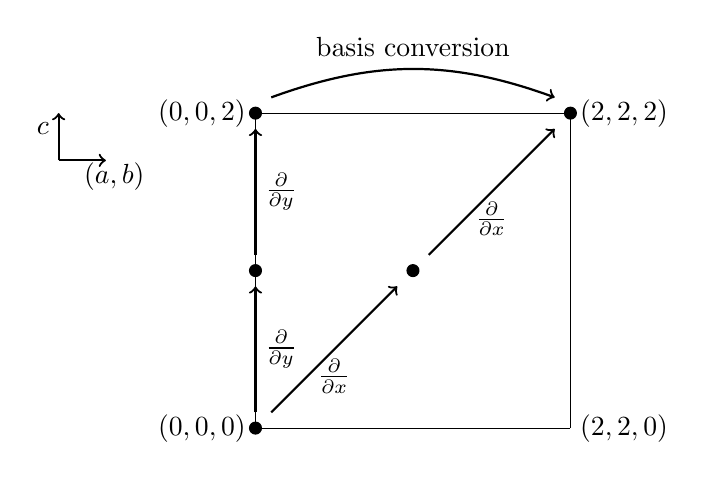
\begin{tikzpicture} 
% Box/square (4x4)
\draw[black,solid,ultra thin] (0,0)--(0,4);
\draw[black,solid,ultra thin] (0,0)--(4,0);
\draw[black,solid,ultra thin] (4,0)--(4,4);
\draw[black,solid,ultra thin] (0,4)--(4,4);
% Dots
\draw[black,fill=black] (0,0) circle (.5ex);
\draw[black,fill=black] (2,2) circle (.5ex);
\draw[black,fill=black] (4,4) circle (.5ex);
\draw[black,fill=black] (0,2) circle (.5ex);
\draw[black,fill=black] (0,4) circle (.5ex);
% Arrows
\draw[black,thick,->] (0.2,0.2)--(1.8,1.8);
\draw[black,thick,->] (2.2,2.2)--(3.8,3.8);
\draw[black,thick,->] (0,0.2)--(0,1.8);
\draw[black,thick,->] (0,2.2)--(0,3.8);
\draw [black,thick,->] (0.2,4.2) to [out=20,in=160] (3.8,4.2);
% Node (parameter) labels
\draw[] (0,0) node[anchor=east] {$(0,0,0)$};
\draw[] (0,4) node[anchor=east] {$(0,0,2)$};
\draw[] (4,0) node[anchor=west] {$(2,2,0)$};
\draw[] (4,4) node[anchor=west] {$(2,2,2)$};
% Arrow labels
\draw[] (1,1) node[anchor=north] {$\tfrac{\partial}{\partial x}$};
\draw[] (3,3) node[anchor=north] {$\tfrac{\partial}{\partial x}$};
\draw[] (0,1) node[anchor=west] {$\tfrac{\partial}{\partial y}$};
\draw[] (0,3) node[anchor=west] {$\tfrac{\partial}{\partial y}$};
% The key and headings
\draw[black,thick,->] (-2.5,3.4)--(-2.5,4);
\draw[black,thick,->] (-2.5,3.4)--(-1.9,3.4);
\draw[] (-2.3,3.2) node[anchor=west] {$(a,b)$};
\draw[] (-2.7,3.6) node[anchor=south] {$c$};
\draw[] (2,4.6) node[anchor=south] {basis conversion};
\end{tikzpicture} 
\caption{The Laplace operator acting on vectors of $\smash{\hdopnk^{(0,0,0)}}$ coefficients has a sparse matrix representation if the range is represented as vectors of $\smash{\hdopnk^{(2,2,2)}}$ coefficients. Here, the arrows indicate that the corresponding operation has a sparse matrix representation when the domain is $\smash{\hdopnkabc}$ coefficients, where $(a,b,c)$ is at the tail of the arrow, and the range is $\smash{\hdopnk^{(\tilde{a},\tilde{b},\tilde{c})}}$ coefficients, where $(\tilde{a},\tilde{b},\tilde{c})$ is at the head of the arrow. %For example, $\smash{\frac{\partial}{\partial x}}$ has a sparse matrix representation when the domain is represented in $\smash{\hdop_{n,k}^{(0,0,0)}}$ (resp.~$\smash{\hdop_{n,k}^{(1,0,1)}}$) and the range in $\smash{\hdop_{n,k}^{(1,0,1)}}$ (resp.~$\smash{\hdop_{n,k}^{(2,0,2)}}$).
}
\label{fig:ds:laplaceparameterconversion} 
\end{figure}


In this section, we concentrate on the disk-slice case, and simply note that similar arguments apply for the trapezium case. Recall that, for the disk-slice,
\bseqn{
	\Omega := \{(x,y) \in \R^2 \quad | \quad \alpha < x < \beta, \: \gamma \rho(x) < y < \delta \rho(x)\}
}
where
\bseqn{
	\begin{cases}
		(\alpha,\beta) &\subset (0,1) \\
		(\gamma,\delta) &:= (-1,1) \\
		\rho(x) &:= (1-x^2)^{\half}
	\end{cases}.
}
The 2D OPs on the disk-slice $\Omega$, orthogonal with respect to the weight
\bseqn{
	\Wabc(x,y) &:= \genjacw^{(a,b,2c)}(x) \: \jacw^{(c)}\fpr(\frac{y}{\rho(x)}) \\
	&= (\beta - x)^a \: (x - \alpha)^b \: (1-x^2-y^2)^c, \quad (x,y) \in \Omega,
}
are then given by:
\bseqn{
	\hdopnkabc(x,y) := \genjacnmk^{(a, b, 2c+2k+1)}(x) \: \rho(x)^k \: \jac_k^{(c,c)}\fpr(\frac{y}{\rho(x)}), \quad (x,y) \in \Omega
}
where the 1D OPs $\{\genjac^{(a, b, c)}_n\}$ are orthogonal on the interval $(\alpha, \beta)$ with respect to the weight
\bseqn{
	\genjacw^{(a,b,c)}(x) :=  (\beta - x)^a \: (x - \alpha)^b \: \rho(x)^{c}
}
and the 1D OPs $\{\jac^{(c, c)}_n\}$ are orthogonal on the interval $(\gamma, \delta) = (-1, 1)$ with respect to the weight
\bseqn{
	\jacw^{(c)}(x) := (1-x)^c \: (1+x)^c = (1-x^2)^c.
}
Denote the weighted OPs by
\bseqn{
	\bigWabc(x,y) := \Wabc(x,y) \: \bighdopabc(x,y),
}
and recall that a function $f(x,y)$ defined on $\Omega$ is approximated by its expansion $f(x,y) = \bighdopabc(x,y)^\top \vec{f}$. 

\begin{definition}\label{def:ds:differentialoperators}
	Define the operator matrices $D_x^{(a,b,c)}, \: D_y^{(a,b,c)}, \: W_x^{(a,b,c)}, \: W_y^{(a,b,c)}$ according to:
\bseqn{
	{\partial f \over \partial x}&= \bighdop^{(a+1,b+1,c+1)}(x,y)^\top \: D_x^{(a,b,c)} \: \vec{f}, \\
	{\partial f \over \partial y} &= \bighdop^{(a,b,c+1)}(x,y)^\top \: D_y^{(a,b,c)} \: \vec{f}, \\
	{\partial \over \partial x}[\Wabc(x,y) \: f(x,y)] &= \bigW^{(a-1,b-1,c-1)}(x,y)^\top \: W_x^{(a,b,c)} \: \vec{f}, \\
	{\partial \over \partial y}[\Wabc(x,y) \: f(x,y)] &= \bigW^{(a,b,c-1)}(x,y)^\top \: W_y^{(a,b,c)} \: \vec{f}.
}
\end{definition}

The incrementing and decrementing of parameters as seen here is analogous to other well known orthogonal polynomial families' derivatives, for example the Jacobi polynomials on the interval, as seen in the DLMF \cite[(18.9.3)]{DLMF}, and on the triangle \cite{olver2018recurrence}. An illustration of how the non-weighted differential operators increment the parameters (a,b,c) is seen in \bsreffig{fig:ds:laplaceparameterconversion}.

\begin{theorem}\label{theorem:ds:sparsityofdifferentialoperators}
	The operator matrices $D_x^{(a,b,c)}, \: D_y^{(a,b,c)}, \: W_x^{(a,b,c)}, \: W_y^{(a,b,c)}$ from \bsrefdef{def:ds:differentialoperators} are sparse, with banded-block-banded structure. More specifically:
\begin{itemize}
	\item $D_x^{(a,b,c)}$ has  block-bandwidths $(-1,3)$, and sub-block-bandwidths $(0, 2)$.
  	\item $D_y^{(a,b,c)}$ has  block-bandwidths $(-1,1)$, and sub-block-bandwidths $(-1,1)$.
	\item $W_x^{(a,b,c)}$ has  block-bandwidths $(3,-1)$, and sub-block-bandwidths $(2, 0)$.
  	\item $W_y^{(a,b,c)}$ has  block-bandwidths $(1,-1)$, and sub-block-bandwidths $(1,-1)$.
\end{itemize}
\end{theorem}

\begin{proof}
First, note that:
\bseqnnumber{
	\genjacw^{(a,b,c) \: \prime}(x) &= - a \: \genjacw^{(a-1,b,c)}(x) + b \: \genjacw^{(a,b-1,c)}(x) + c \: \rho(x) \: \rho'(x) \:\genjacw^{(a,b,c-2)}(x), \label{eqn:ds:derivativeofweightgenjac} \\
	\jacw^{(c) \: \prime}(y) &= - 2c \: y \: \jacw^{(c-1)}(y), \label{eqn:ds:derivativeofweightjac} \\
	\rho(x) \: \rho'(x) &= -x. \label{eqn:ds:rhoderivative}
}
We proceed with the case for the operator $D_y^{(a,b,c)}$ for partial differentiation by $y$. Since $\{\hdop^{(a,b,c+1)}_{m,j}\}$ for $m = 0,\dots,n-1$, $j = 0,\dots,m$ is an orthogonal basis for any degree $n-1$ polynomial, we can expand $\ppx{y} \hdopnkabc = \sum_{m=0}^{n-1} \sum_{j=0}^m c_{m,j}^y \: \hdop^{(a, b, c+1)}_{m,j}$. The coefficients of the expansion are then the entries of the relevant operator matrix. We can use an integration-by-parts argument to show that the only non-zero coefficient of this expansion is when $m = n-1$, $j = k-1$. First, note that
\bseqn{
	c_{m,j}^y = {\ip<\ppx{y} \hdopnkabc, \hdop^{(a, b, c+1)}_{m,j} >_{W^{(a, b, c+1)}}}{\norm{\hdop^{(a, b, c+1)}_{m,j}}^{-2}_{W^{(a, b+1)}}}.
}
Then, using the change of variable $t = \frac{y}{\rho(x)}$, we have that
\bseqn{
	&\ip<\ppx{y} \hdopnkabc, \hdop^{(a, b, c+1)}_{m,j} >_{W^{(a, b, c+1)}} \\
	&= \iint_\Omega \: \Big[ \genjacnmk^{(a,b,2c+2k+1)}(x) \: \rho(x)^{k-1} \: \jac_k^{(c,c) \: \prime}\fpr(\frac{y}{\rho(x)}) \\
	& \quad \quad \quad \quad \quad \quad \cdot \: \genjacmmj^{(a,b,2c+2j+3)}(x) \: \rho(x)^{j} \: \jac_j^{(c+1,c+1)}\fpr(\frac{y}{\rho(x)}) \Big] \: \D y \: \D x \\
	&= \normgenjac^{(a, b, 2c+2k+1)} \: \ip< \genjacnmk^{(a,b,2c+2k+1)}, \rho(x)^{j-k+1} \: \genjacmmj^{(a,b,2c+2j+3)} >_{\genjacw^{(a,b,2c+2k+1)}} \\
	&\quad \quad \quad \quad \quad \quad \cdot \: \normjac^{(c+1)} \: \ip< \jac_k^{(c,c) \: \prime}, \: \jac_{j}^{(c+1,c+1)} >_{\jacw^{(c+1)}}
}
Now, using \bsrefeqn{eqn:ds:derivativeofweightjac}, integration-by-parts, and noting that the weight $\jacw^{(c)}$ is a polynomial of degree $2c$ and vanishes at the limits of the integral for positive parameter $c$, we have that
\bseqn{
	&\normjac^{(c+1)} \: \ip< \jac_k^{(c,c) \: \prime}, \: \jac_{j}^{(c+1,c+1)} >_{\jacw^{(c+1)}} \\
	&= \int_{\gamma}^\delta \: \jac_k^{(c,c) \: \prime}(y) \: \jac_{j}^{(c+1,c+1)}(y) \: \jacw^{(c+1)}(y) \: \D y \\
	&= - \int_{-1}^1 \: \jac_k^{(c,c)}(y) \: \ddx{y} [\jacw^{(c+1)}(y) \: \jac_{j}^{(c+1,c+1)}(y)] \: \D y \\
	&= - \int_{-1}^1 \: \jac_k^{(c,c)} \: [ \jac_{j}^{(c+1,c+1) \: \prime} \: \jacw^{(c+1)} - 2 c \: y \: \jac_{j}^{(c+1,c+1)} \:\jacw^{(c)} ] \: \D y \\
	&= - \: \normjac^{(c)} \: \ip< \jac_k^{(c,c)}, \: \jacw^{(1)} \: \jac_{j}^{(c+1,c+1) \: \prime} -2c \:y \: \jac_{j}^{(c+1,c+1)} >_{\jacw^{(c)}}
}
which is zero for $j < k-1$ by orthogonality. Further, when $j = k-1$, we have that
\bseqn{
	&\normgenjac^{(a, b, 2c+2k+1)} \: \ip< \genjacnmk^{(a,b,2c+2k+1)}, \rho(x)^{j-k+1} \: \genjacmmj^{(a,b,2c+2j+3)} >_{\genjacw^{(a,b,2c+2k+1)}} \\
	&= \normgenjac^{(a, b, 2c+2k+1)} \: \ip< \genjacnmk^{(a,b,2c+2k+1)}, \genjacmmj^{(a,b,2c+2k+1)} >_{\genjacw^{(a,b,2c+2k+1)}} \\
	&= \normgenjac^{(a, b, 2c+2k+1)} \: \delta_{n,m+1},
}
showing that the only possible non-zero coefficient is when $m=n-1, j=k-1$. Finally,
\bseqn{
	c_{n-1,k-1}^y &= \ip< \jac_k^{(c,c) \: \prime}, \: \jac_{k-1}^{(c+1,c+1)} >_{\jacw^{(c+1)}}.
}

We next consider the case for the operator $D_x^{(a,b,c)}$ for partial differentiation by $x$. Since $\{\hdop^{(a+1, b+1, c+1)}_{m,j}\}$ for $m = 0,\dots,n-1$, $j = 0,\dots,m$ is an orthogonal basis for any degree $n-1$ polynomial, we can expand $\ppx{x} \hdopnkabc = \sum_{m=0}^{n-1} \sum_{j=0}^m c_{m,j}^x \: \hdop^{(a+1, b+1, c+1)}_{m,j}$. The coefficients of the expansion are then the entries of the relevant operator matrix. As before, we can use an integration-by-parts argument to show that the only non-zero coefficients of this expansion are when $m = n-1, n-2, n-3$, $j = k, k-1, k-2$ and $0 \le j \le m$. First, note that
\bseqn{
	c_{m,j}^x = {\ip<\ppx{x} \hdopnkabc, \hdop^{(a+1, b+1, c+1)}_{m,j} >_{W^{(a+1, b+1, c+1)}}}{\norm{\hdop^{(a+1, b+1, c+1)}_{m,j}}^{-2}_{W^{(a+1, b+1, c+1)}}}.
}
Now, again using the change of variable $t= \frac{y}{\rho(x)}$, we have that
\bseqnnumber{
	&\ip<\ppx{x} \hdopnkabc, \hdop^{(a+1, b+1, c+1)}_{m,j} >_{W^{(a+1, b+1, c+1)}} \nonumber \\ 
	&= \Big( \int_\alpha^\beta \: \genjacnmk^{(a, b, 2c+2k+1) \: \prime} \: \genjacmmj^{(a+1, b+1, 2c+2j+3)} \: \rho^{k+j+1} \: \genjacw^{(a+1, b+1, 2c+2)} \: \D x \Big) \nonumber \\
	&\quad \quad \quad \quad \quad \cdot \: \Big( \int_\gamma^\delta \jac_k^{(c,c)} \: \jac_j^{(c+1,c+1)} \: \jacw^{(c+1)} \: \D t \Big) \nonumber \\ 
	& \quad + k \: \Big( \int_\alpha^\beta \: \genjacnmk^{(a, b, 2c+2k+1)} \: \genjacmmj^{(a+1, b+1, 2c+2j+3)} \: \rho^{k+j} \: \rho' \: \genjacw^{(a+1, b+1, 2c+2)} \: \D x \Big) \nonumber \\
	& \quad \quad \quad \quad \quad \cdot \: \Big( \int_\gamma^\delta \jac_k^{(c,c)} \: \jac_j^{(c+1,c+1)} \: \jacw^{(c+1)} \: \D t \Big) \nonumber \\
	& \quad - \Big( \int_\alpha^\beta \: \genjacnmk^{(a, b, 2c+2k+1)} \: \genjacmmj^{(a+1, b+1, 2c+2j+3)} \: \rho^{k+j} \: \rho' \: \genjacw^{(a+1, b+1, 2c+2)} \: \D x \Big) \nonumber \\
	& \quad \quad \quad \quad \quad \cdot \: \Big( \int_\gamma^\delta t \: \jac_k^{(c,c) \: \prime} \: \jac_j^{(c+1,c+1)} \: \jacw^{(c+1)} \: \D t \Big). \label{eqn:ds:dxsparsity}
}
We will first show that the second factor of each term in \bsrefeqn{eqn:ds:dxsparsity} are zero for $j < k - 2$ and also for $j = k - 1$. To this end, observe that, for any integer $c$, $\jac^{(c,c)}(-t) = (-1)^k \: \jac^{(c,c)}(t)$ and so $\jac_k^{(c,c)}$ is an even polynomial for even $k$, and an odd polynomial for odd $k$. Thus, $\jac_k^{(c,c)} \: \jac_{k-1}^{(c+1,c+1)}$ is an odd polynomial for any $k$. Hence
\bseqn{
	\int_\gamma^\delta \jac_k^{(c,c)} \: \jac_j^{(c+1,c+1)} \: \jacw^{(c+1)} \: \D t = \int_{-\delta}^\delta \jac_k^{(c,c)} \: \jac_j^{(c+1,c+1)} \: \jacw^{(1)} \: \jacw^{(c)} \: \D t 
}
is zero for $j < k - 2$ by orthogonality, and is zero for $j = k-1$ due to symmetry over the domain. Moreover, $t \: \jac_k^{(c,c) \: \prime}(t) \: \jac_j^{(c+1,c+1)}(t)$ is also an odd polynomial for any $k$ and so
\bseqn{
	\int_\gamma^\delta t \: \jac_k^{(c,c) \: \prime}(t) \: \jac_j^{(c+1,c+1)}(t) \: \jacw^{(c+1)}(t) \: \D t
}
is zero for $j = k-1$ due to symmetry over the domain, and
\bseqn{
	&\int_\gamma^\delta t \: \jac_k^{(c,c) \: \prime} \: \jac_j^{(c+1,c+1)} \: \jacw^{(c+1)} \: \D t \\
	&= - \int_{-\delta}^\delta \jac_k^{(c,c)} \: \frac{\D}{\D t} \big[ t \: \jac_j^{(c+1,c+1)} \: \jacw^{(c+1)} \big] \: \D t \\
	&= - \int_{-\delta}^\delta \jac_k^{(c,c)} \: \big[ \jac_j^{(c+1,c+1)} \: \jacw^{(c+1)} + t \: \jac_j^{(c+1,c+1) \: \prime} \: \jacw^{(c+1)} - 2 c \: t^2 \: \jac_j^{(c+1,c+1)} \: \jacw^{(c)} \big] \: \D t \\
	&= - \: \normjac^{(c)} \: \ip< \jac_k^{(c,c)}, \: \jac_j^{(c+1,c+1)} \: \jacw^{(1)} + t \: \jac_{j}^{(c+1,c+1) \: \prime} \: \jacw^{(1)} - 2c \: t^2 \: \jac_{j}^{(c+1,c+1)}  >_{\jacw^{(c)}}
}
which is zero for $j < k - 2$ by orthogonality. Thus, \bsrefeqn{eqn:ds:dxsparsity} is zero for $j \notin \{k-2, k\}$.

Now, using \bsrefeqn{eqn:ds:derivativeofweightgenjac}, integration-by-parts, and noting that the weight $\genjacw^{(a,b,2c)}$ is a polynomial degree $a+b+2c$ and vanishes at the limits of the integral for positive parameters $a,b,c$, we have that
\bseqnnumber{
	&\int_\alpha^\beta \: \genjacnmk^{(a, b, 2c+2k+1) \: \prime} \: \genjacmmj^{(a+1, b+1, 2c+2j+3)} \: \rho^{k+j+1} \: \genjacw^{(a+1, b+1, 2c+2)} \: \D x \nonumber  \\
	&= \int_\alpha^\beta \: \genjacnmk^{(a, b, 2c+2k+1) \: \prime} \: \genjacmmj^{(a+1, b+1, 2c+2j+3)} \: \genjacw^{(a+1, b+1, 2c+k+j+3)} \: \D x \nonumber \\
	&= - \int_\alpha^\beta \: \genjacnmk^{(a, b, 2c+2k+1)} \: \ddx{x} \Big[ \genjacmmj^{(a+1, b+1, 2c+2j+3)} \: \genjacw^{(a+1, b+1, 2c+k+j+3)} \Big] \: \D x \nonumber \\
	&= - \int_\alpha^\beta \: \genjacnmk^{(a, b, 2c+2k+1)} \: \Big\{ \genjacmmj^{(a+1, b+1, 2c+2j+3) \: \prime} \: \genjacw^{(a+1, b+1, 2c+k+j+3)} \nonumber \\
		&\quadeight + (2c+k+j+3) \: \rho \: \rho' \:  \genjacw^{(a+1, b+1, 2c+k+j+1)} \: \genjacmmj^{(a+1, b+1, 2c+2j+3)} \nonumber \\
		&\quadeight + (b+1) \: \genjacw^{(a+1, b, 2c+k+j+3)} \: \genjacmmj^{(a+1, b+1, 2c+2j+3)} \nonumber \\
		&\quadeight - (a+1) \: \genjacw^{(a, b+1, 2c+k+j+3)} \: \genjacmmj^{(a+1, b+1, 2c+2j+3)} \Big\} \: \D x \nonumber \\
	&= - \: \normgenjac^{(a, b, 2c+2k+1)} \:  \Big\{ \ip<\genjacnmk^{(a, b, 2c+2k+1)}, \: \genjacw^{(1, 1, j-k+2)} \: \genjacmmj^{(a+1, b+1, 2c+2j+3) \: \prime}>_{\genjacw^{(a, b, 2c+2k+1)}} \nonumber \\
		&\quad + (2c+k+j+3) \ip<\genjacnmk^{(a, b, 2c+2k+1)}, \: \rho \rho' \: \genjacw^{(1,1, j-k)} \genjacmmj^{(a+1, b+1, 2c+2j+3)} >_{\genjacw^{(a, b, 2c+2k+1)}} \nonumber \\
		&\quad + (b+1) \ip<\genjacnmk^{(a, b, 2c+2k+1)}, \: \genjacw^{(1,0, j-k+2)} \genjacmmj^{(a+1, b+1, 2c+2j+3)} >_{\genjacw^{(a, b, 2c+2k+1)}} \nonumber \\
		&\quad - (a+1) \ip<\genjacnmk^{(a, b, 2c+2k+1)}, \: \genjacw^{(0,1, j-k+2)} \genjacmmj^{(a+1, b+1, 2c+2j+3)} >_{\genjacw^{(a, b, 2c+2k+1)}} \Big\}. \label{eqn:ds:dxsparsityR}
}
By recalling \bsrefeqn{eqn:ds:rhoderivative} and noting that $j-k$ is even by the earlier argument, we can see $\rho \: \rho' \: \genjacw^{(1,1, j-k)}$, $\genjacw^{(1,0, j-k+2)}$ and $\genjacw^{(1,0, j-k+2)}$ are all polynomials, and further that 
\bseqn{
	\deg(\rho \rho' \: \genjacw^{(1,1, j-k)}) = \deg(\genjacw^{(1,0, j-k+2)}) = \deg(\genjacw^{(0,1, j-k+2)}) = 3 + j-k.
}
Hence, by orthogonality, each term in \bsrefeqn{eqn:ds:dxsparsityR} is is zero for $m-j+3+j-k < n-k \iff m < n - 3$.

Finally,
\bseqn{
	&\int_\alpha^\beta \: \genjacnmk^{(a, b, 2c+2k+1)} \: \genjacmmj^{(a+1, b+1, 2c+2j+3)} \: \rho^{k+j} \: \rho' \: \genjacw^{(a+1, b+1, 2c+2)} \: \D x \\
	&= \normgenjac^{(a, b, 2c+2k+1)} \: \ip< \genjacnmk^{(a, b, 2c+2k+1)}, \: \rho \: \rho' \: \genjacw^{(1, 1, j-k)} \: \genjacmmj^{(a+1, b+1, 2c+2j+3)} >_{\genjacw^{(a, b, 2c+2k+1)}}
}
which is also zero for $m < n - 3$. Thus
\bseqn{
	&\ip<\ppx{x} \hdopnkabc, \hdop^{(a+1, b+1, c+1)}_{m,j} >_{W^{(a+1, b+1, c+1)}} = 0
}
for $m < n - 3$, $j \notin \{k-2, k\}$, showing that the only possible non-zero coefficients $c_{m,j}^x$ are when $m = n-3,n-2,n-1$ and $j = k-2,k$ $(j \le m)$.

We can gain the non-zero entries of the weighted differential operators similarly, by noting that for the disk-slice
\bseqnnumber{
	\ppx{x} \Wabc(x,y) &= -a W^{(a-1, b, c)}(x,y) + bW^{(a, b, c)}(x,y) + 2c \rho(x) \: \rho'(x) \: W^{(a, b, c-1)} \label{eqn:ds:weightderivativex} \\
	\ppx{y} \Wabc(x,y) &= -2c \: y \: W^{(a, b, c-1)}(x,y) \label{eqn:ds:weightderivativey}
}
and also that
\bseqn{
	\ip< \Wabc \hdopnkabc, W^{(\tilde{a},\tilde{b},\tilde{c})} \hdopmj^{(\tilde{a},\tilde{b},\tilde{c})} >_{W^{(-\tilde{a},-\tilde{b},-\tilde{c})}} = \ip< \hdopnkab, \hdopmj^{(\tilde{a},\tilde{b})} >_\Wabc.
}
\end{proof}

There exist conversion matrix operators that increment/decrement the parameters, transforming the OPs from one (weighted or non-weighted) parameter space to another. 

\begin{definition}\label{def:ds:parametertransformationoperators}
	Define the operator matrices 
\bseqn{
	T^{(a,b,c)\to(a+1,b+1,c)}, \quad T^{(a,b,c)\to(a,b,c+1)}\qqand T^{(a,b,c)\to(a+1,b+1,c+1)}
}
for conversion between non-weighted spaces, and 
\bseqn{
	T_W^{(a,b,c)\to(a-1,b-1,c)}, \quad T_W^{(a,b,c)\to(a,b,c-1)} \qqand T_W^{(a,b,c)\to(a-1,b-1,c-1)}
}
for conversion between weighted spaces, according to:
\bseqn{
	\bighdop^{(a,b,c)}(x,y) &= \Big(T^{(a,b,c)\to(a+1,b+1,c)} \Big)^\top \: \bighdop^{(a+1,b+1,c)}(x,y) \\
	\bighdop^{(a,b,c)}(x,y) &= \Big(T^{(a,b,c)\to(a,b,c+1)} \Big)^\top \: \bighdop^{(a,b,c+1)}(x,y) \\
	\bighdop^{(a,b,c)}(x,y) &= \Big(T^{(a,b,c)\to(a+1,b+1,c+1)} \Big)^\top \: \bighdop^{(a+1,b+1,c+1)}(x,y) \\
	\bigW^{(a,b,c)}(x,y) &= \Big(T_W^{(a,b,c)\to(a-1,b-1,c)} \Big)^\top \: \bigW^{(a-1,b-1,c)}(x,y) \\
	\bigW^{(a,b,c)}(x,y) &= \Big(T_W^{(a,b,c)\to(a,b,c-1)} \Big)^\top \: \bigW^{(a,b,c-1)}(x,y) \\
	\bigW^{(a,b,c)}(x,y) &= \Big(T_W^{(a,b,c)\to(a-1,b-1,c-1)} \Big)^\top \: \bigW^{(a-1,b-1,c-1)}(x,y).
}
\end{definition}

\begin{lemma}\label{lemma:ds:sparsityofparametertransformationoperators}
	The operator matrices in \bsrefdef{def:ds:parametertransformationoperators} are sparse, with banded-block-banded structure. More specifically:
\begin{itemize}
	\item $T^{(a,b,c)\to(a+1,b+1,c)}$ has block-bandwidth $(0,2)$, with diagonal blocks.
  	\item $T^{(a,b,c)\to(a,b,c+1)}$ has block-bandwidth $(0,2)$ and sub-block-bandwidth $(0,2)$.
	\item $T^{(a,b,c)\to(a+1,b+1,c+1)}$ has block-bandwidth $(0,4)$ and sub-block-bandwidth $(0,2)$.
	\item $T_W^{(a,b,c)\to(a-1,b-1,c)}$ has block-bandwidth $(2,0)$ with diagonal blocks.
  	\item $T_W^{(a,b,c)\to(a,b,c-1)}$ has block-bandwidth $(2,0)$ and sub-block-bandwidth $(2,0)$.
	\item $T_W^{(a,b,c)\to(a-1,b-1,c-1)}$ has block-bandwidth $(4,0)$ and sub-block-bandwidth $(2,0)$.
\end{itemize}
\end{lemma}

\begin{proof}
We proceed with the case for the non-weighted operators $T^{(a,b)\to(a+\tilde{a},b+\tilde{b},c+\tilde{c})}$, where $\tilde{a}, \tilde{b}, \tilde{c} \in \{0,1\}$. Since $\{\hdop^{(a+\tilde{a},b+\tilde{b},c+\tilde{c})}_{m,j}\}$ for $m = 0,\dots,n$, $j = 0,\dots,m$ is an orthogonal basis for any degree $n$ polynomial, we can expand $\hdopnkabc = \sum_{m=0}^{n} \sum_{j=0}^m c_{m,j} \: \hdop^{(a+\tilde{a},b+\tilde{b},c+\tilde{c})}_{m,j}$. The coefficients of the expansion are then the entries of the relevant operator matrix. We will show that the only non-zero coefficients are for $m \ge n - \tilde{a} - \tilde{b} - 2\tilde{c} $, $j \ge k-2\tilde{c}$ and $0 \le j \le m$. First, note that
\bseqn{
	c_{m,j} = {\ip< \hdopnkabc, \hdop^{(a+\tilde{a},b+\tilde{b},c+\tilde{c})}_{m,j} >_{W^{(a+\tilde{a},b+\tilde{b},c+\tilde{c})}}}{\norm{\hdop^{(a+\tilde{a},b+\tilde{b},c+\tilde{c})}_{m,j}}^{-2}_{W^{(a+\tilde{a},b+\tilde{b},c+\tilde{c})}}}.
}
Then, using the change of variable $t = \frac{y}{\rho(x)}$, we have that
\bseqn{
	&\ip< \hdopnkabc, \hdop^{(a+\tilde{a},b+\tilde{b},c+\tilde{c})}_{m,j} >_{W^{(a+\tilde{a},b+\tilde{b},c+\tilde{c})}} \\
	&= \normgenjac^{(a+\tilde{a},b+\tilde{b},2c+2\tilde{c})} \: \ip< \genjacnmk^{(a,b,2c+2k+1)}, \rho(x)^{k+j+1} \: \genjacmmj^{(a+\tilde{a},b+\tilde{b},2c+2\tilde{c}+2j+1)} >_{\genjacw^{(a+\tilde{a},b+\tilde{b},2c+2\tilde{c})}} \\ 
		&\quadfour \cdot \: \normjac^{(c+\tilde{c})} \: \ip< \jac_k^{(c,c)}, \: \jac_{j}^{(c+\tilde{c},c+\tilde{c})} >_{\jacw^{(c+\tilde{c})}} \\
	&= \normgenjac^{(a,b,2c+2k+1)} \: \ip< \genjacnmk^{(a,b,2c+2k+1)}, \genjacw^{(\tilde{a}, \tilde{b}, \: 2\tilde{c}+j-k)} \: \genjacmmj^{(a+\tilde{a},b+\tilde{b},2c+2\tilde{c}+2j+1)} >_{\genjacw^{(a,b,2c+2k+1)}} \\
		&\quadfour \cdot \: \normjac^{(c)} \: \ip< \jac_k^{(c,c)}, \: \jacw^{(\tilde{c})} \: \jac_{j}^{(c+\tilde{c},c+\tilde{c})} >_{\jacw^{(c)}}.
}
Since $\jacw^{(\tilde{c})}$ is a polynomial degree $2\tilde{c}$, we have that the above is then zero for $j < k-2\tilde{c}$. Further, since $\genjacw^{(\tilde{a}, \tilde{b}, \: 2\tilde{c}+j-k)}$ is a polynomial of degree $\tilde{a}+\tilde{b}+2\tilde{c}+j-k$, we have that the above is zero for $m-j+\tilde{a}+\tilde{b}+2\tilde{c}+j-k < n-k \iff m < n - \tilde{a}-\tilde{b}-2\tilde{c}$.

The sparsity argument for the weighted parameter transformation operators follows similarly.
\end{proof}

\begin{figure}[tp]
	\centering % <-- added
	\begin{subfigure}{0.5\textwidth}
		\centerline{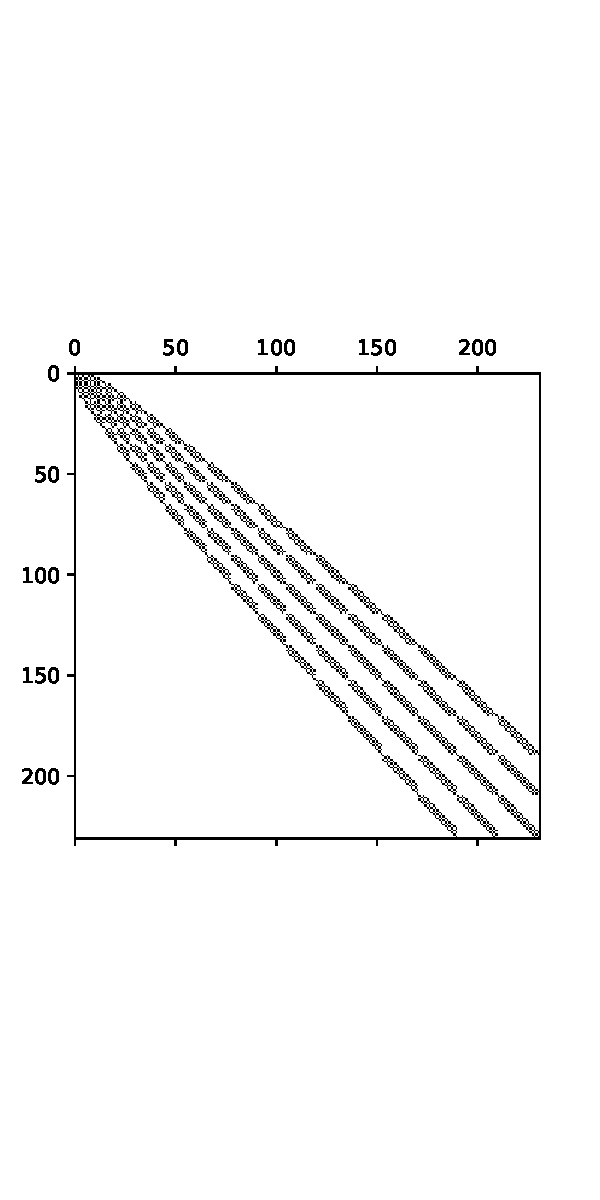
\includegraphics[scale=0.5]{sparsityoflaplacian-w11-diskslice-alpha=0p2-beta=0p8}}
		\centering
		\caption{}
	\end{subfigure}\hfil % <-- added
	\begin{subfigure}{0.5\textwidth}
		\centerline{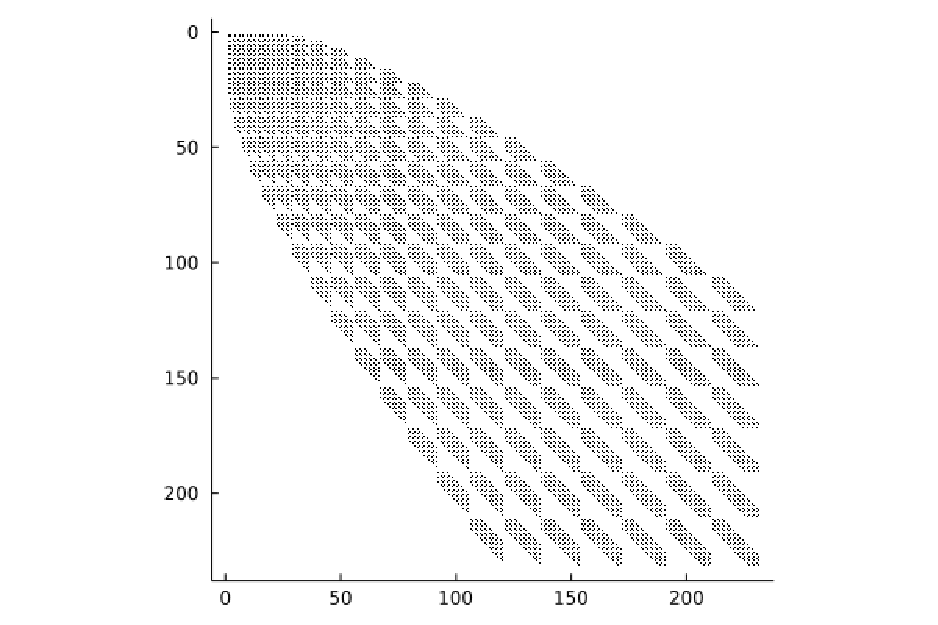
\includegraphics[scale=0.5]{sparsityofhelmholtz-diskslice-alpha=0p2-beta=0p8}}
		\centering
		\caption{}
	\end{subfigure}\hfil % <-- added

	\medskip
	\begin{subfigure}{0.5\textwidth}
		\centerline{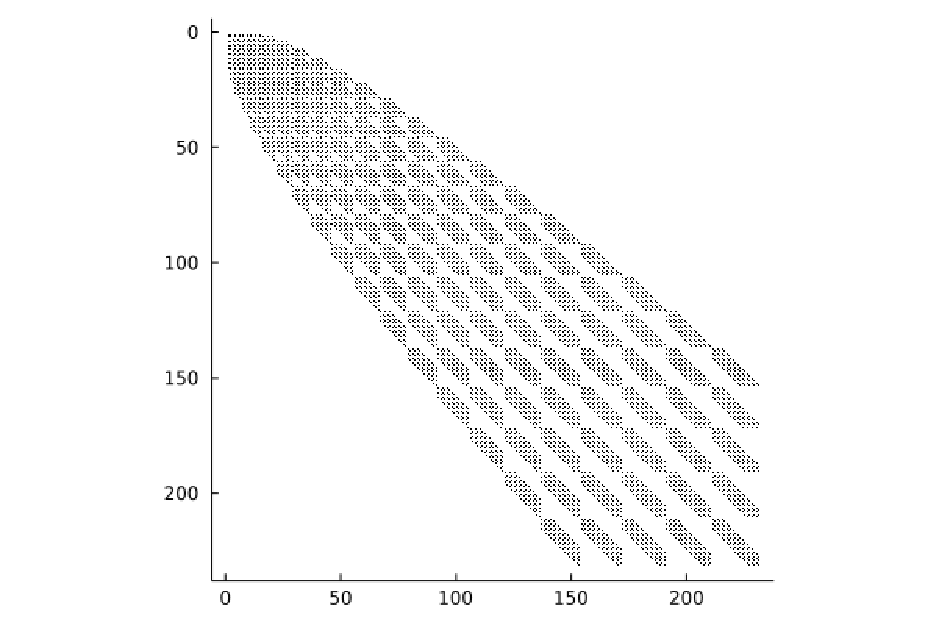
\includegraphics[scale=0.5]{sparsityofbiharmonic-diskslice-alpha=0p2-beta=0p8}}
		\centering
		\caption{}
	\end{subfigure}\hfil % <-- added
    	\caption{"Spy" plots of (differential) operator matrices, showing their sparsity. (a) The Laplacian operator $\laplacewiii$. (b) The variable coefficient Helmholtz operator $\laplacewiii + k^2 \: T^{(0,0,0)\to(1,1,1)} \: V({J_x^{(0,0,0)}}^\top, {J_y^{(0,0,0)}}^\top) \: T_W^{(1,1,1)\to(0,0,0)}$ for $v(x,y) = 1 - (3(x-1)^2 + 5y^2)$ and $k = 200$. (c) The biharmonic operator $\biharmonictwo$}
	\label{fig:ds:sparsity}
\end{figure}

General linear partial differential operators with polynomial variable coefficients can be constructed by composing the sparse representations for partial derivatives, conversion between bases, and Jacobi operators. As a canonical example, we can obtain the matrix operator for the Laplacian $\Delta$, that will take us from coefficients for expansion in the weighted space
\bseqn{
	\bigWiii(x,y) = \Wiii(x,y) \: \bighdopiii(x,y)
}
to coefficients in the non-weighted space $\bighdopiii(x,y)$. Note that this construction will ensure the imposition of the Dirichlet zero boundary conditions on $\Omega$. The matrix operator for the Laplacian we denote $\laplacewiii$ acting on the coefficients vector is then given by
\bseqn{
    \laplacewiii := D_x^{(0,0,0)} \: W_x^{(1,1,1)} + T^{(0,0,1)\to(1,1)} \: D_y^{(0,0,0)} \: T_W^{(1,1,0)\to(0,0,0)} \: W_y^{(1,1,1)}.
}
Importantly, this operator will have banded-block-banded structure, and hence will be sparse, as seen in \bsreffig{fig:ds:sparsity}.

Another important example is the Biharmonic operator $\Delta^2$, where we assume zero Dirichlet and Neumann conditions. To construct this operator, we first note that we can obtain the matrix operator for the Laplacian $\Delta$ that will take us from coefficients for expansion in the space $\bighdopooo(x,y)$ to coefficients in the space $\bighdop^{(2,2,2)}(x,y)$. We denote this matrix operator that acts on the coefficients vector as $\laplaceooo$, and is given by
\bseqn{
    \laplaceooo := D_x^{(1,1,1)} \: D_x^{(0,0,0)} + T^{(1,1,2)\to(2,2,2)} \: D_y^{(1,1,1)} \: T^{(0,0,1)\to(1,1,1)} \: D_y^{(0,0,0)}.
}
Further, we can represent the Laplacian as a map from coefficients in the space $\bigW^{(2,2)}$ to coefficients in the space $\bighdopooo$. Note that a function expanded in the $\bigW^{(2,2)}$ basis will satisfy both zero Dirichlet and Neumann boundary conditions on $\Omega$. We denote this matrix operator as $\laplacewttt$, and is given by
\bseqn{
	\laplacewttt := W_x^{(1,1,1)} \: W_x^{(2,2,2)} + T_W^{(1,1,0)\to(0,0,0)} \: W_y^{(1,1,1)} \: T_W^{(2,2,1)\to(1,1,1)} \: W_y^{(2,2,2)}.
}
We can then construct a matrix operator for $\Delta^2$ that will take coefficients in the space $\bigW^{(2,2,2)}$ to coefficients in the space $\bighdop^{(2,2,2)}$. Note that any function expanded in the $\bigW^{(2,2,2)}$ basis will satisfy both zero Dirichlet and zero Neumann boundary conditions on $\Omega$. The matrix operator for the Biharmonic operator is then given by
\bseqn{
	\biharmonictwo = \laplaceooo \: \laplacewttt.
}
The sparsity and structure of this biharmonic operator are seen in \bsreffig{fig:ds:sparsity}.



\section{Computational aspects}\label{Section:Computation}

In this section we discuss how to take advantage of the proposed basis and sparsity structure in partial differential operators in practical computational applications.

\subsection{Constructing $\genjac_n^{(a,b,c)}(x)$}

%To obtain the recurrence coefficients for the $\{\genjac_n^{(a,b,c)}\}$ OPs in (\ref{eqn:Hrecurrence}), we use a variant of the Stieltjes procedure \cite{gautschi1982generating} where the polynomials are expressed as Chebyshev polynomial expansions and the inner products are calculated via Clenshaw--Curtis quadrature. This has the benefit that it is easier to incorporate high-precision arithmetic, which we use to overcome ill-conditioning present when $c$ is large, as required for large $n$ in \eqref{eq:diskpolys}. The ApproxFun.jl \cite{ApproxFun} package gives a convenient way to manipulate Chebyshev and Jacobi expansions, which we use to calculate the inner products and norms in this algorithm, utilising the {\tt BigFloat} type to handle high-precision calculations.


It is possible to obtain the recurrence coefficients for the $\{\genjac_n^{(a,b,c)}\}$ OPs in \bsrefeqn{eqn:ds:Hrecurrence}, by careful application of the Christoffel--Darboux formula \cite[18.2.12]{DLMF}. We explain the process here for the disk-slice case, however we note that a similar but simpler argument holds for the trapezium case. We thus first need to define a new set of `interim' 1D OPs.
\begin{definition}\label{def:ds:InterimOPconstruction}
Let $\genjactw^{(a,b,c,d)}(x) := (\beta - x)^a \: (x - \alpha)^{b} \: (1-x)^{c} \: (1+x)^{d} $ be a weight function on the interval $(\alpha, \beta)$, and define the associated inner product by:
\bseqnnumber{
	\ip< p, \: q >_{\genjactw^{(a,b,c,d)}} &:= \frac{1}{\normgenjact^{(a,b,c,d)}} \: \int_\alpha^\beta p(x) \: q(x) \: \genjactw^{(a,b,c,d)}(x) \: \D x \label{eqn:ds:ipgenjact}
}
where
\bseqnnumber{
	\normgenjact^{(a,b,c,d)} := \int_\alpha^\beta \: \genjactw^{(a,b,c,d)}(x) \: \D x
}
Denote the four-parameter family of orthonormal polynomials on $[\alpha,\beta]$ by $\{\genjact_n^{(a,b,c,d)}\}$, orthonormal with respect to the inner product defined in \bsrefeqn{eqn:ds:ipgenjact}.
\end{definition}
Note that the OPs $\{\genjac_n^{(a,b,2c)}\}$ are then equivalent to the OPs $\{\genjact_n^{(a,b,c,c)}\}$. Let the recurrence coefficients for the OPs $\{\genjact_n^{(a,b,c,d)}\}$ be given by:
\bseqnnumber{
	x \: \genjact_n^{(a,b,c,d)}(x) = \tilde{\beta}_n^{(a,b,c,d)} \: \genjact_{n+1}^{(a,b,c,d)}(x) + \tilde{\alpha}_n^{(a,b,c,d)} \:\genjact_n^{(a,b,c,d)}(x) + \tilde{\beta}_{n-1}^{(a,b,c,d)} \: \genjact_{n-1}^{(a,b,c,d)}(x)
}
\begin{proposition}
There exist constants $\mathcal{C}_n^{(a,b,c,d)}$, $\mathcal{D}_n^{(a,b,c,d)}$ such that
\bseqnnumber{
	\genjact_n^{(a,b,c+1,d)}(x) &= \mathcal{C}_n^{(a,b,c,d)} \: \sum_{k=0}^n \: \genjact_{k}^{(a,b,c,d)}(1) \: \genjact_{k}^{(a,b,c,d)}(x) \label{eqn:ds:genjacexpansioni} \\
	\genjact_n^{(a,b,c,d+1)}(x) &= \mathcal{D}_n^{(a,b,c,d)} \: \sum_{k=0}^n \: \genjact_{k}^{(a,b,c,d)}(-1) \: \genjact_{k}^{(a,b,c,d)}(x) \label{eqn:ds:genjacexpansionii}
}
\end{proposition}

\begin{proof}
Fix $n,m \in \{0,1,\dots\}$ and without loss of generality, assume $m \le n$. First recall that
\bseqn{
	\int_\alpha^\beta \: \genjact_n^{(a,b,c+1,d)}(x) \: \genjact_m^{(a,b,c+1,d)}(x) \: \genjactw^{(a,b,c+1,d)}(x) \: \D x &= \delta_{n,m} \: \normgenjact^{(a,b,c+1,d)}
}
and define
\bseqnnumber{
	\mathcal{C}_n^{(a,b,c,d)} &= \fpr(\frac{\normgenjact^{(a,b,c+1,d)}}{\normgenjact^{(a,b,c,d)} \: \genjact_n^{(a,b,c,d)}(1) \: \genjact_{n+1}^{(a,b,c,d)}(1) \: \tilde{\beta}_n^{(a,b,c,d)}})^\half, \label{eqn:ds:genjactnormalisationi} \\
	\mathcal{D}_n^{(a,b,c,d)} &= (-1)^n \: \fpr(\frac{- \normgenjact^{(a,b,c,d+1)}}{\normgenjact^{(a,b,c,d)} \: \genjact_n^{(a,b,c,d)}(-1) \: \genjact_{n+1}^{(a,b,c,d)}(-1) \: \tilde{\beta}_n^{(a,b,c,d)}})^\half. \label{eqn:ds:genjactnormalisationii}
}
Now, by the Christoffel--Darboux formula \cite[18.2.12]{DLMF}, we have that for any $x, y \in \R$,
\bseqnnumber{
	&\sum_{k=0}^n \: \genjact_{k}^{(a,b,c,d)}(y) \: \genjact_{k}^{(a,b,c,d)}(x) \nonumber \\
	&= \tilde{\beta}_n^{(a,b,c,d)} \: \frac{\genjact_{n}^{(a,b,c,d)}(x) \: \genjact_{n+1}^{(a,b,c,d)}(y) - \genjact_{n+1}^{(a,b,c,d)}(x) \: \genjact_{n}^{(a,b,c,d)}(y)}{y - x}. \label{eqn:ds:christoffeldarboux}
}
Then,
\bseqn{
	&\int_\alpha^\beta \: \Big(\big[\mathcal{C}_n^{(a,b,c,d)} \: \sum_{k=0}^n \: \genjact_{k}^{(a,b,c,d)}(1) \: \genjact_{k}^{(a,b,c,d)}(x)\big] \\
		&\quadfour \cdot \big[\mathcal{C}_m^{(a,b,c,d)} \: \sum_{k=0}^m \: \genjact_{k}^{(a,b,c,d)}(1) \: \genjact_{k}^{(a,b,c,d)}(x)\big] \: \genjactw^{(a,b,c+1,d)}(x) \Big) \: \D x \\
	&= \mathcal{C}_n^{(a,b,c,d)} \: \mathcal{C}_m^{(a,b,c,d)} \: \tilde{\beta}_n^{(a,b,c,d)} \\
		&\quad \cdot \sum_{k=0}^m \: \int_\alpha^\beta \genjactw^{(a,b,c,d)}(x) \Big\{ \genjact_{k}^{(a,b,c,d)}(1) \: \genjact_{k}^{(a,b,c,d)}(x) \\
		&\quadeight \quadtwo \cdot \big[\genjact_{n}^{(a,b,c,d)}(x) \: \genjact_{n+1}^{(a,b,c,d)}(1) - \genjact_{n+1}^{(a,b,c,d)}(x) \: \genjact_{n}^{(a,b,c,d)}(1)\big] \Big\} \: \D x \\
	&= \delta_{m,n} \: {\mathcal{C}_n^{(a,b,c,d)}}^2 \: \tilde{\beta}_n^{(a,b,c,d)} \: \normgenjact^{(a,b,c,d)} \: \genjact_{n}^{(a,b,c,d)}(1) \: \genjact_{n+1}^{(a,b,c,d)}(1) \\
	&= \delta_{m,n} \: \normgenjact^{(a,b,c+1,d)}
}
using \bsrefeqn{eqn:ds:genjactnormalisationi} and \bsrefeqn{eqn:ds:christoffeldarboux}, showing that the RHS and LHS of \bsrefeqn{eqn:ds:genjacexpansioni} are equivalent. Further,
\bseqn{
	&\int_\alpha^\beta \Big\{ \big[\mathcal{D}_n^{(a,b,c,d)} \: \sum_{k=0}^n \: \genjact_{k}^{(a,b,c,d)}(-1) \: \genjact_{k}^{(a,b,c,d)}(x)\big] \\
		&\quadfour \cdot \big[\mathcal{D}_m^{(a,b,c,d)} \: \sum_{k=0}^m \: \genjact_{k}^{(a,b,c,d)}(-1) \: \genjact_{k}^{(a,b,c,d)}(x)\big] \: \genjactw^{(a,b,c,d+1)}(x) \Big\} \: \D x \\
	&= - \mathcal{D}_n^{(a,b,c,d)} \: \mathcal{D}_m^{(a,b,c,d)} \: \tilde{\beta}_n^{(a,b,c,d)} \\
		&\quad \cdot \sum_{k=0}^m \: \int_\alpha^\beta \genjactw^{(a,b,c,d)}(x) \Big\{ \genjact_{k}^{(a,b,c,d)}(-1) \: \genjact_{k}^{(a,b,c,d)}(x) \\
		&\quadeight \cdot \big[\genjact_{n}^{(a,b,c,d)}(x) \: \genjact_{n+1}^{(a,b,c,d)}(-1) - \genjact_{n+1}^{(a,b,c,d)}(x) \: \genjact_{n}^{(a,b,c,d)}(-1)\big] \Big\} \: \D x \\
	&= - \delta_{m,n} \: {\mathcal{D}_n^{(a,b,c,d)}}^2 \: \tilde{\beta}_n^{(a,b,c,d)} \: \normgenjact^{(a,b,c,d)} \: \genjact_{n}^{(a,b,c,d)}(-1) \: \genjact_{n+1}^{(a,b,c,d)}(-1) \\
	&= \delta_{m,n} \: \normgenjact^{(a,b,c,d+1)}
}
using \bsrefeqn{eqn:ds:genjactnormalisationii} and \bsrefeqn{eqn:ds:christoffeldarboux}, showing that the RHS and LHS of \bsrefeqn{eqn:ds:genjacexpansionii} are also equivalent. 
\end{proof}

\begin{proposition}
The recurrence coefficients for the OPs $\{\genjact_n^{(a,b,c+1,d)}\}$ are given by:
\bseqnnumber{
	\tilde{\alpha}_n^{(a,b,c+1,d)} &= \frac{\genjact_{n+2}^{(a,b,c,d)}(1)}{\genjact_{n+1}^{(a,b,c,d)}(1)} \: \tilde{\beta}_{n+1}^{(a,b,c,d)} - \frac{\genjact_{n+1}^{(a,b,c,d)}(1)}{\genjact_{n}^{(a,b,c,d)}(1)} \: \tilde{\beta}_{n}^{(a,b,c,d)} + \tilde{\alpha}_{n+1}^{(a,b,c,d)}, \\
	\tilde{\beta}_n^{(a,b,c+1,d)} &= \frac{\mathcal{C}_n^{(a,b,c,d)}}{\mathcal{C}_{n+1}^{(a,b,c,d)}} \: \frac{\genjact_{n}^{(a,b,c,d)}(1)}{\genjact_{n+1}^{(a,b,c,d)}(1)} \: \tilde{\beta}_n^{(a,b,c,d)}.
}
The recurrence coefficients for the OPs $\{\genjact_n^{(a,b,c,d+1)}\}$ are given by:
\bseqnnumber{
	\tilde{\alpha}_n^{(a,b,c,d+1)} &= \frac{\genjact_{n+2}^{(a,b,c,d)}(-1)}{\genjact_{n+1}^{(a,b,c,d)}(-1)} \: \tilde{\beta}_{n+1}^{(a,b,c,d)} - \frac{\genjact_{n+1}^{(a,b,c,d)}(-1)}{\genjact_{n}^{(a,b,c,d)}(-1)} \: \tilde{\beta}_{n}^{(a,b,c,d)} + \tilde{\alpha}_{n+1}^{(a,b,c,d)}, \\
	\tilde{\beta}_n^{(a,b,c,d+1)} &= \frac{\mathcal{D}_n^{(a,b,c,d)}}{\mathcal{D}_{n+1}^{(a,b,c,d)}} \: \frac{\genjact_{n}^{(a,b,c,d)}(-1)}{\genjact_{n+1}^{(a,b,c,d)}(-1)} \: \tilde{\beta}_n^{(a,b,c,d)}.
}
\end{proposition}

\begin{proof}
First, using \bsrefeqn{eqn:ds:genjacexpansioni} and \bsrefeqn{eqn:ds:christoffeldarboux} we have that
\bseqnnumber{
	&(1-x) \: x \: \genjact_{n}^{(a,b,c+1,d)}(x) \nonumber \\
	&= \mathcal{C}_n^{(a,b,c,d)} \: \tilde{\beta}_{n}^{(a,b,c,d)} \: x \: \Big[\genjact_{n}^{(a,b,c,d)}(x) \: \genjact_{n+1}^{(a,b,c,d)}(1) - \genjact_{n+1}^{(a,b,c,d)}(x) \: \genjact_{n}^{(a,b,c,d)}(1)\Big] \nonumber \\
	&= \mathcal{C}_n^{(a,b,c,d)} \: \tilde{\beta}_{n}^{(a,b,c,d)} \nonumber \\
		&\quad \cdot \Big\{  \genjact_{n+1}^{(a,b,c,d)}(1) \: \Big(\tilde{\beta}_{n}^{(a,b,c,d)} \genjact_{n+1}^{(a,b,c,d)}(x) + \tilde{\alpha}_{n}^{(a,b,c,d)} \genjact_{n}^{(a,b,c,d)}(x) \nonumber \\
			&\quadeight \quad + \tilde{\beta}_{n-1}^{(a,b,c,d)} \genjact_{n-1}^{(a,b,c,d)}(x)\Big) \nonumber \\
		&\quadfour - \genjact_{n}^{(a,b,c,d)}(1) \: \Big(\tilde{\beta}_{n+1}^{(a,b,c,d)} \genjact_{n+2}^{(a,b,c,d)}(x) + \tilde{\alpha}_{n+1}^{(a,b,c,d)} \genjact_{n+1}^{(a,b,c,d)}(x) \nonumber \\
			&\quadeight \quadfour + \tilde{\beta}_{n}^{(a,b,c,d)} \genjact_{n}^{(a,b,c,d)}(x)\Big) \Big\} \label{eqn:ds:genjactproofa}
}
Next, note that the recurrence coefficients for $\genjact_{n}^{(a,b,c+1,d)}(x)$ satisfy
\bseqnnumber{
	&(1-x) \: x \: \genjact_{n}^{(a,b,c+1,d)}(x) \nonumber \\
	&= (1-x) \: \Big\{ \tilde{\beta}_{n}^{(a,b,c+1,d)} \genjact_{n+1}^{(a,b,c+1,d)}(x) + \tilde{\alpha}_{n}^{(a,b,c+1,d)} \genjact_{n}^{(a,b,c+1,d)}(x) \nonumber \\
		&\quadeight + \tilde{\beta}_{n-1}^{(a,b,c+1,d)} \genjact_{n-1}^{(a,b,c+1,d)}(x) \Big\} \nonumber \\
	&= \mathcal{C}_{n+1}^{(a,b,c,d)} \tilde{\beta}_{n}^{(a,b,c+1,d)} \tilde{\beta}_{n+1}^{(a,b,c,d)} \: \Big( \genjact_{n+1}^{(a,b,c,d)}(x) \genjact_{n+2}^{(a,b,c,d)}(1) - \genjact_{n+2}^{(a,b,c,d)}(x) \genjact_{n+1}^{(a,b,c,d)}(1) \Big) \nonumber \\
		&\quad + \mathcal{C}_n^{(a,b,c,d)} \tilde{\alpha}_{n}^{(a,b,c+1,d)} \tilde{\beta}_{n}^{(a,b,c,d)} \: \Big( \genjact_{n}^{(a,b,c,d)}(x) \genjact_{n+1}^{(a,b,c,d)}(1) - \genjact_{n+1}^{(a,b,c,d)}(x) \genjact_{n}^{(a,b,c,d)}(1) \Big) \nonumber \\
		&\quad + \mathcal{C}_{n-1}^{(a,b,c,d)} \tilde{\beta}_{n-1}^{(a,b,c+1,d)} \tilde{\beta}_{n-1}^{(a,b,c,d)} \: \Big( \genjact_{n-1}^{(a,b,c,d)}(x) \genjact_{n}^{(a,b,c,d)}(1) - \genjact_{n}^{(a,b,c,d)}(x) \genjact_{n-1}^{(a,b,c,d)}(1) \Big) \label{eqn:ds:genjactproofb}
}
We can set $\tilde{\beta}_{-1}^{(a,b,c+1,d)} = 0$. By comparing coefficients of $\genjact_{n+2}^{(a,b,c,d)}(x)$ and $\genjact_{n+1}^{(a,b,c,d)}(x)$ in both \bsrefeqn{eqn:ds:genjactproofa} and \bsrefeqn{eqn:ds:genjactproofb} we obtain the desired recurrence coefficients for the OP $\genjact_{n}^{(a,b,c+1,d)}(x)$. The recurrence coefficients for the OPs $\genjact_{n}^{(a,b,c,d+1)}(x)$ are found similarly.
\end{proof}

\begin{corollary}
The recurrence coefficients for the OPs $\{\genjact_n^{(a,b,c+1,d)}\}$ can be written as:
\bseqnnumber{
	\tilde{\alpha}_n^{(a,b,c+1,d)} &= \frac{\tilde{\beta}_{n-1}^{(a,b,c,d)}}{\chi_{n-1}^{(a,b,c,d)}(1)} - \frac{\tilde{\beta}_{n}^{(a,b,c,d)}}{\chi_{n}^{(a,b,c,d)}(1)} + \tilde{\alpha}_{n}^{(a,b,c,d)}, \\
	\tilde{\beta}_n^{(a,b,c+1,d)} &= \fpr(\frac{1 - \tilde{\alpha}_{n+1}^{(a,b,c,d)} - \frac{\tilde{\beta}_n^{(a,b,c,d)}}{\chi_n^{(a,b,c,d)}(1)}}{1 - \tilde{\alpha}_{n}^{(a,b,c,d)} - \frac{\tilde{\beta}_{n-1}^{(a,b,c,d)}}{\chi_{n-1}^{(a,b,c,d)}(1)}})^\half \tilde{\beta}_n^{(a,b,c,d)}.
}
The recurrence coefficients for the OPs $\{\genjact_n^{(a,b,c,d+1)}\}$ can be written as:
\bseqnnumber{
	\tilde{\alpha}_n^{(a,b,c,d+1)} &= \frac{\tilde{\beta}_{n-1}^{(a,b,c,d)}}{\chi_{n-1}^{(a,b,c,d)}(-1)} - \frac{\tilde{\beta}_{n}^{(a,b,c,d)}}{\chi_{n}^{(a,b,c,d)}(-1)} + \tilde{\alpha}_{n}^{(a,b,c,d)}, \\
	\tilde{\beta}_n^{(a,b,c,d+1)} &= \fpr(\frac{- 1 + \tilde{\alpha}_{n+1}^{(a,b,c,d)} + \frac{\tilde{\beta}_n^{(a,b,c,d)}}{\chi_n^{(a,b,c,d)}(-1)}}{- 1 + \tilde{\alpha}_{n}^{(a,b,c,d)} + \frac{\tilde{\beta}_{n-1}^{(a,b,c,d)}}{\chi_{n-1}^{(a,b,c,d)}(-1)}})^\half \tilde{\beta}_n^{(a,b,c,d)}.
}
where 
\bseqnnumber{
	\chi_{n}^{(a,b,c,d)}(y) &:= \frac{\genjact_{n+1}^{(a,b,c,d)}(y)}{\genjact_{n}^{(a,b,c,d)}(y)} \\
	&= \frac{1}{\tilde{\beta}_{n}^{(a,b,c,d)}} \: \fpr(y - \tilde{\alpha}_{n}^{(a,b,c,d)} - \frac{\tilde{\beta}_{n-1}^{(a,b,c,d)}}{\chi_{n-1}^{(a,b,c,d)}(y)}), \quad y \in \{-1,1\}.
}
\end{corollary}

These two propositions allow us to recursively obtain the recurrence coefficients for the OPs $\{\genjac_{n-k}^{(a,b,2c+2k + 1)}\}$ as $k$ increases to be large. 

\noindent{\bf Remark}:
The Corollary demonstrates that in order to obtain the recurrence coefficients $\{\alpha_{m}^{(a,b,2c+2k+1)}\}$, $\{\beta_{m}^{(a,b,2c+2k+1)}\}$ for some $m$ and $k$, we require that we obtain the recurrence coefficients $\{\alpha_{m+2}^{(a,b,2c+2(k-1)+1)}\}$, $\{\beta_{m+2}^{(a,b,2c+2(k-1)+1)}\}$. Thus, for large $N$, this recursive method of obtaining the recurrence coefficients requires a large initialisation (i.e. using the Lanczos algorithm to compute the recurrence coefficients $\{\alpha_{n}^{(a,b,2c+1)}\}$, $\{\beta_{n}^{(a,b,2c+1)}\}$ -- however, we only need to compute these once, and can store and save this initialisation to disk once computed, for the given values of $a, b, c$). 
%This is the most expensive part of the current calculation, but note that we can reuse this computation for multiple partial differential equations. Efficient construction of OPs with large parameters in the weights is an important topic, but one tangential to the proposed scheme. 

\subsection{Quadrature rule on the disk-slice}

In this section we construct a quadrature rule exact for polynomials in the disk-slice $\Omega$ that can be used to expand functions in $\hdopnkabc(x,y)$ when $\Omega$ is a disk-slice.

\begin{theorem}
Denote the  Gauss quadrature nodes and weight on $[\alpha,\beta]$ with weight $(\beta - s)^a \: (s - \alpha)^b \: \rho(s)^{2c+1}$ as $(s_k,w_k^{(s)})$ , and
 on \([-1,1]\) with weight \((1-t^2)^c\) as $(t_k,w_k^{(t)})$. Define
\bseqn{
	x_{i+(j-1)N} &:= s_j, \quad i,j = 1,\dots, \ceil{\frac{N+1}{2}}, \\
	y_{i+(j-1)N} &:= \rho(s_j) \: t_i, \quad i,j = 1,\dots, \ceil{\frac{N+1}{2}}, \\
	w_{i+(j-1)N} &:= w_j^{(s)} w_i^{(t)}, \quad  i,j = 1,\dots, \ceil{\frac{N+1}{2}}.
}
Let $f(x,y)$ be a polynomial on $\Omega$. The quadrature rule is then
$$
\iint_\Omega f(x,y) \: \Wab(x,y) \: \D A \approx \half \sum_{j=1}^{M} w_j \: \big[ f(x_j, y_j) + f(x_j, -y_j) \big],
$$
where $M = \ceil{\half(N+1)}^2$, and the quadrature rule is exact if $f(x,y)$ is a polynomial of degree $\le N$.
\end{theorem}

\begin{proof}
We will use the substitution that
\bseqn{
	x &= s, \quad y = \rho(s) \: t.
}
First, note that, for $(x,y) \in \Omega$,
\bseqn{
	\Wabc(x,y) &= \genjacw^{(a,b,2c)}(x) \: \jacw^{(c)}\fpr(\frac{y}{\rho(x)}) \\
	&= \genjacw^{(a,b,c2)}(s) \: \jacw^{(c)}(t) \\
	&=: V^{(a,b,c)}(s,t), \quad \text{for } (s,t) \in [\alpha,\beta] \times [-1,1].
}

Let $f : \Omega \to \R$. Define the functions $f_e, f_o : \Omega \to \R$ by 
\bseqn{
	f_e(x,y) &:= \half \Big(f(x, y) + f(x, -y)\Big), \quad \forall (x,y) \in \Omega\\
	f_o(x,y) &:= \half \Big(f(x, y) - f(x, -y)\Big), \quad \forall (x,y) \in \Omega
}
so that $y \mapsto f_e(x,y)$ for fixed $x$ is an even function, and $y \mapsto f_o(x,y)$ for fixed $x$ is an odd function. Note that if $f$ is a polynomial, then $f_e(s, \rho(s)t)$ is a polynomial in $s \in [\alpha,\beta]$ for fixed $t$. 

Now, we have that
\bseqn{
	&\iint_\Omega f_e(x,y) \: \Wabc(x,y) \: \D y \: \D x \\
	&\quadfour = \int_\alpha^\beta \int_{-1}^1 f_e\big(s,\rho(s) t\big) \: V^{(a,b,c)}(s,t) \: \rho(s) \: \D t \: \D s \\
	&\quadfour = \int_\alpha^\beta \genjacw^{(a,b,2c+1)}(s) \: \Big( \int_{-1}^1 f_e\big(s,\rho(s) t\big) \: \jacw^{(c)}(t) \: \D t \Big) \: \D s \\
	&\quadfour \approx \int_\alpha^\beta \genjacw^{(a,b,2c+1)}(s) \: \sum_{i=1}^{M_2} \Big( w_i^{(t)} f_e\big(s,\rho(s) t_i\big) \Big) \: \D s \quad (\star) \\
	&\quadfour \approx \sum_{j=1}^{M_1} \Bigg( w_j^{(s)} \: \sum_{i=1}^{M_2} \Big( w_i^{(t)} f_e\big(s_j,\rho(s_j) t_i\big) \Big) \Bigg) \quad (\star \star) \\
	&\quadfour = \sum_{k=1}^{M_1 M_2}  w_k \: f_e(x_k, y_k).
}
Suppose $f$ is a polynomial in $x$ and $y$ of degree $N$, and hence that $f_e$ is a degree $\le N$ polynomial. First, note that the degree of the polynomial given by $x \mapsto f_e(x,y)$ for fixed $y$ is $\le N$ and the degree of the polynomial given by $y \mapsto f_e(x,y)$ for fixed $x$ is $\le N$. Also note that $s \mapsto f_e\big(s,\rho(s) t\big)$ for fixed $t$ is then a degree $N$ polynomial (since $\rho$ is a degree $1$ polynomial). Hence, we achieve equality at $(\star)$ if $2M_2 - 1 \ge N$ and we achieve equality at $(\star \star)$ if also $2M_1 - 1 \ge N$.

Next, note that 
\bseqn{
	&\iint_\Omega f_o(x,y) \: \Wabc(x,y) \: \D y \: \D x \\
	&\quadfour = \int_\alpha^\beta \int_{-1}^1 f_o\big(s,\rho(s) t\big) \: V^{(a,b,c)}(s,t) \: \rho(s) \: \D t \: \D s \\
	&\quadfour = \int_\alpha^\beta  \genjacw^{(a,b,2c+1)}(s) \: \Big( \int_{-1}^1 f_o\big(s,\rho(s) t\big) \: \jacw^{(c)}(t) \: \D t \Big) \: \D s \quad (\dagger) \\
	&\quadfour = 0
}
since the inner integral at $(\dagger)$ over $t$ is zero, due to the symmetry over the domain.

Hence, for a polynomial $f$ in $x$ and $y$ of degree $N$,
\bseqn{
	\iint_\Omega f(x,y) \: \Wabc(x,y) \: \D y \: \D x &= \iint_\Omega \Big(f_e(x,y) + f_o(x,y)\Big) \: \Wabc(x,y) \: \D y \: \D x \\
	&= \iint_\Omega f_e(x,y) \: \Wabc(x,y) \: \D y \: \D x \\
	&= \sum_{j=1}^{M}  w_j \: f_e(x_j, y_j),
}
where $M = \ceil{\half(N+1)}^2$.
\end{proof}

\subsection{Obtaining the coefficients for expansion of a function on the disk-slice}

Fix $a,b,c \in \R$. Then for any function $f : \Omega \to \R$ we can express $f$ by
\bseqn{
	f(x,y) \approx \sum_{n=0}^N \bighdop_n^{(a,b,c)}(x,y)^\top \: \vec{f}_n
}
for N sufficiently large, where
\bseqn{
	\bighdop^{(a,b,c)}_n(x,y) &:= \begin{pmatrix}
		\hdop^{(a,b,c)}_{n,0}(x,y) \\
		\vdots \\
		\hdop^{(a,b,c)}_{n,n}(x,y)
	\end{pmatrix} \in \R^{n+1}
}
for all $n = 0,1,2,\dots,N$, and where
\bseqn{
	\vec{f}_n &:= \begin{pmatrix}
		f_{n,0} \\
		\vdots \\
		f_{n,n}
	\end{pmatrix} \in \R^{n+1} \quad \forall n = 0,1,2,\dots,N, \quad
	f_{n,k} := \frac{\ip< f, \: \hdopnk^{(a,b,c)}>_{\Wabc}}{\norm{\hdopnk^{(a,b,c)}}_{\Wabc}}
}
Recall from \bsrefeqn{eqn:ds:normhdop} that $\norm{\hdopnkabc}^2_\Wabc = \normgenjac^{(a,b,2c+2k+1)} \: \normjac^{(c)}$. Using the quadrature rule detailed in Section 4.2 for the inner product, we can calculate the coefficients $f_{n,k}$ for each $n = 0,\dots,N$, $k = 0,\dots,n$: 
\bseqn{
	f_{n,k} &= \lambda^{(a,b,c)}_k \: \sum_{j=1}^{M} w_j \: \big[ f(x_j, y_j) \: \hdopnkabc(x_j, y_j) +f(x_j, -y_j) \: \hdopnkabc(x_j, -y_j) \big]
}
where $\lambda^{(a,b,c)}_k := {1 \over 2 \: \normgenjac^{(a,b,2c+2k+1)} \: \normjac^{(c)}}$ and $M = \ceil{\half(N+1)}^2$.


\subsection{Calculating non-zero entries of the operator matrices}\label{subsection:Computation-operatormatrices}

The proofs of \bsreftheorem{theorem:ds:sparsityofdifferentialoperators} and \bsreflemma{lemma:ds:sparsityofparametertransformationoperators} provide a way to calculate the non-zero entries of the operator matrices given in \bsrefdef{def:ds:differentialoperators} and \bsrefdef{def:ds:parametertransformationoperators}. We can simply use quadrature to calculate the 1D inner products, which has a complexity of $\bigO(N^3)$. This proves much cheaper computationally than using the 2D quadrature rule to calculate the 2D inner products, which has a complexity of $\bigO(N^4)$. 


%
\section{Examples on the disk-slice with zero Dirichlet conditions}\label{Section:Examples}

We now demonstrate how the sparse linear systems constructed as above can be used to efficiently solve PDEs with zero Dirichlet conditions. We consider Poisson, inhomogeneous variable coefficient Helmholtz equation and the Biharmonic equation, demonstrating the versatility of the approach. 

\subsection{Poisson}

% FIGURES
\begin{figure}[t]
	\begin{subfigure}{0.3\textwidth}
		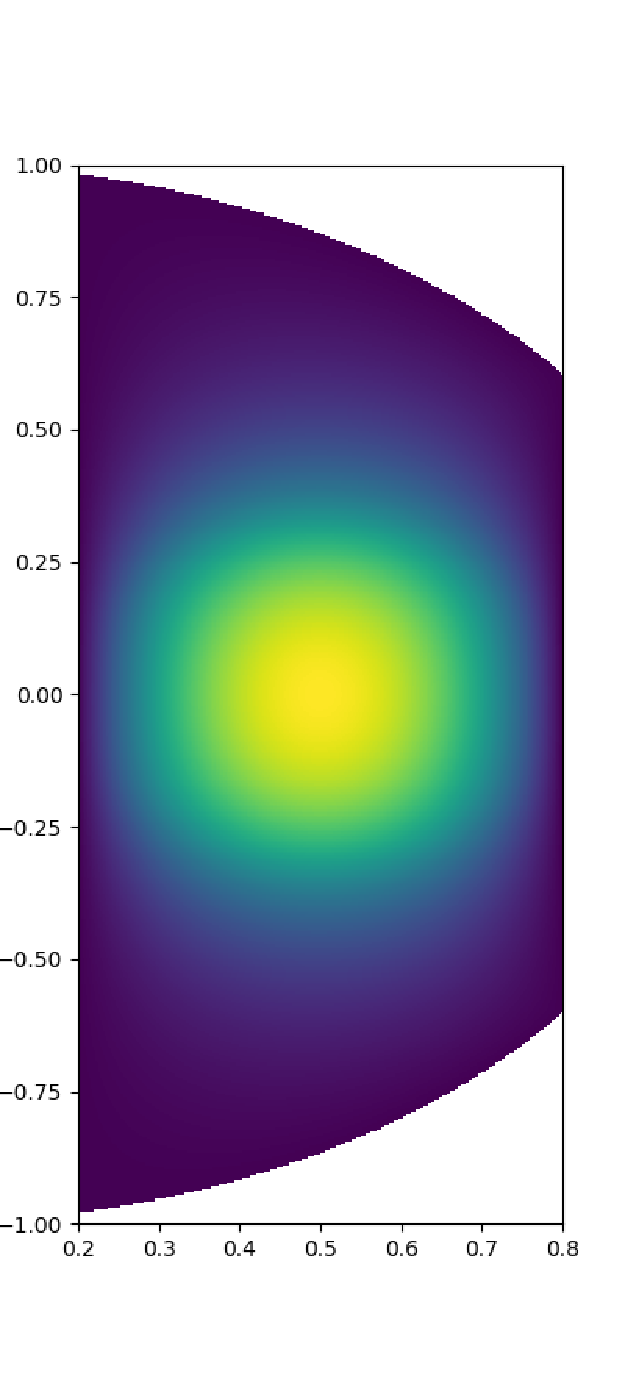
\includegraphics[scale=0.35]{solution-poisson-diskslice-alpha=0p2-beta=0p8}
		\centering
		%\label{fig:ds:solution-poisson}
	\end{subfigure}
	\begin{subfigure}{0.5\textwidth}
		\centering
		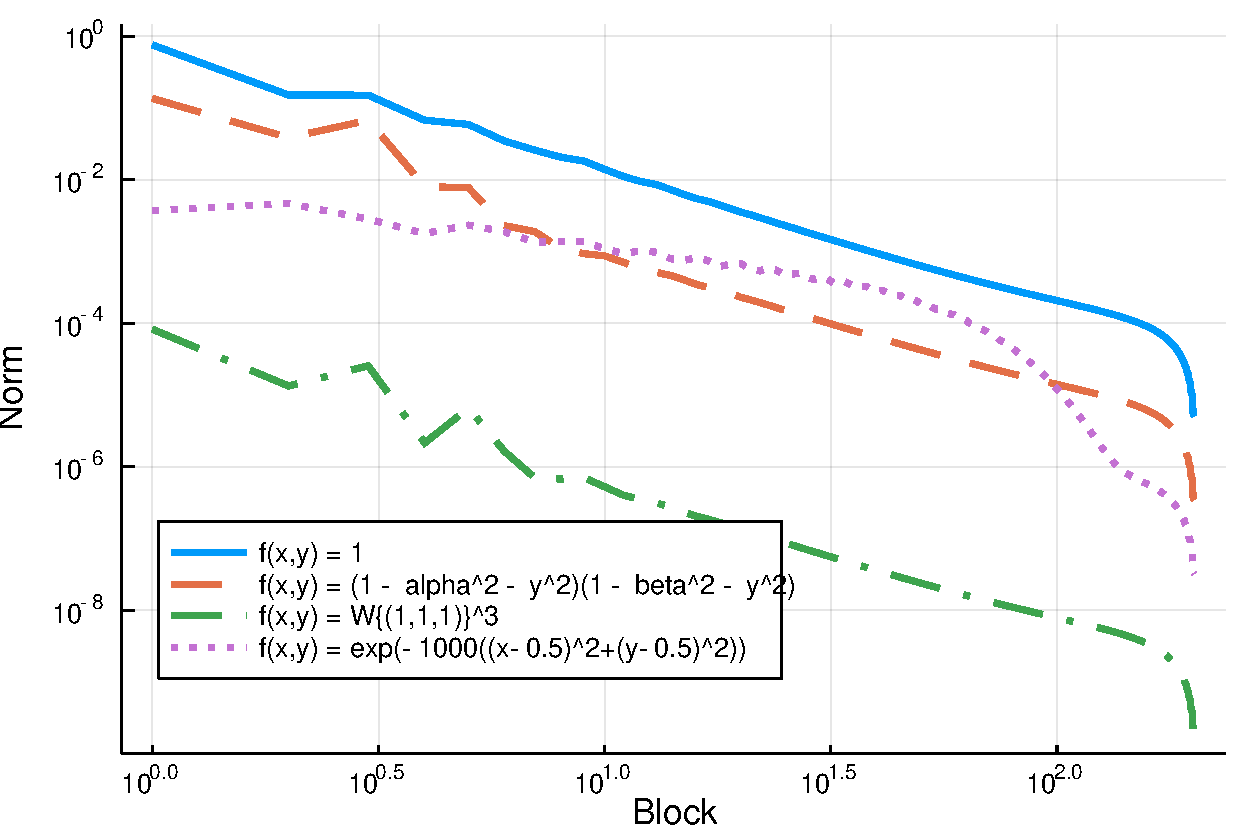
\includegraphics[scale=0.45]{solutionblocknorms-poisson-diskslice-alpha=0p2-beta=0p8-N=200}
        		%\label{fig:ds:solutionblocknorms-poisson}
	\end{subfigure}
	\caption{Left: The computed solution to $\Delta u = f$ with zero boundary conditions with $f(x,y) = 1 + \text{erf}(5(1 - 10((x - 0.5)^2 + y^2)))$. Right: The norms of each block of the computed solution of the Poisson equation with the given right hand side functions. This demonstrates algebraic convergence with the rate dictated by the decay at the corners, with spectral convergence observed when the right-hand side vanishes to all orders.}
	\centering
	\label{fig:ds:poisson}
\end{figure}

\begin{figure}[t]
	\begin{subfigure}{0.3\textwidth}
	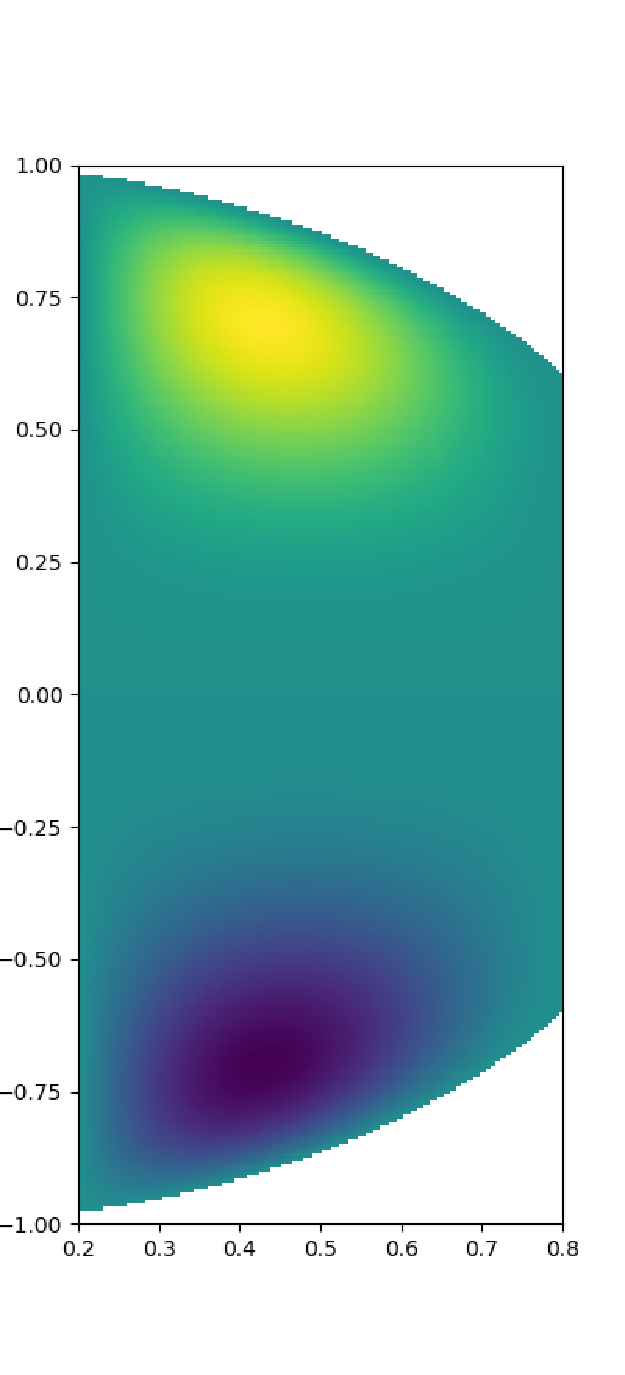
\includegraphics[scale=0.35]{solution-exact-poisson-diskslice-alpha=0p2-beta=0p8-u=y3expx}
	\centering
	\end{subfigure}
	\begin{subfigure}{0.3\textwidth}
	\centering
	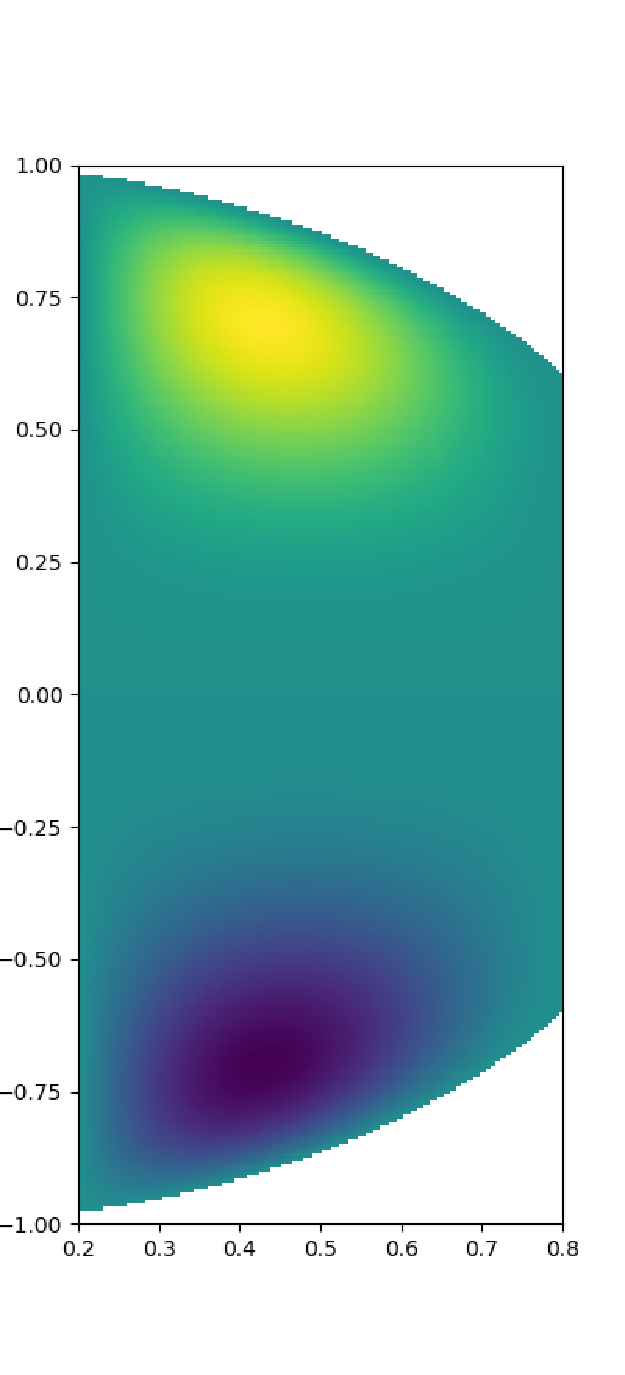
\includegraphics[scale=0.35]{solution-exact-poisson-diskslice-alpha=0p2-beta=0p8-u=y3expx-actual}
	\centering
	\end{subfigure}
	\begin{subfigure}{0.3\textwidth}
	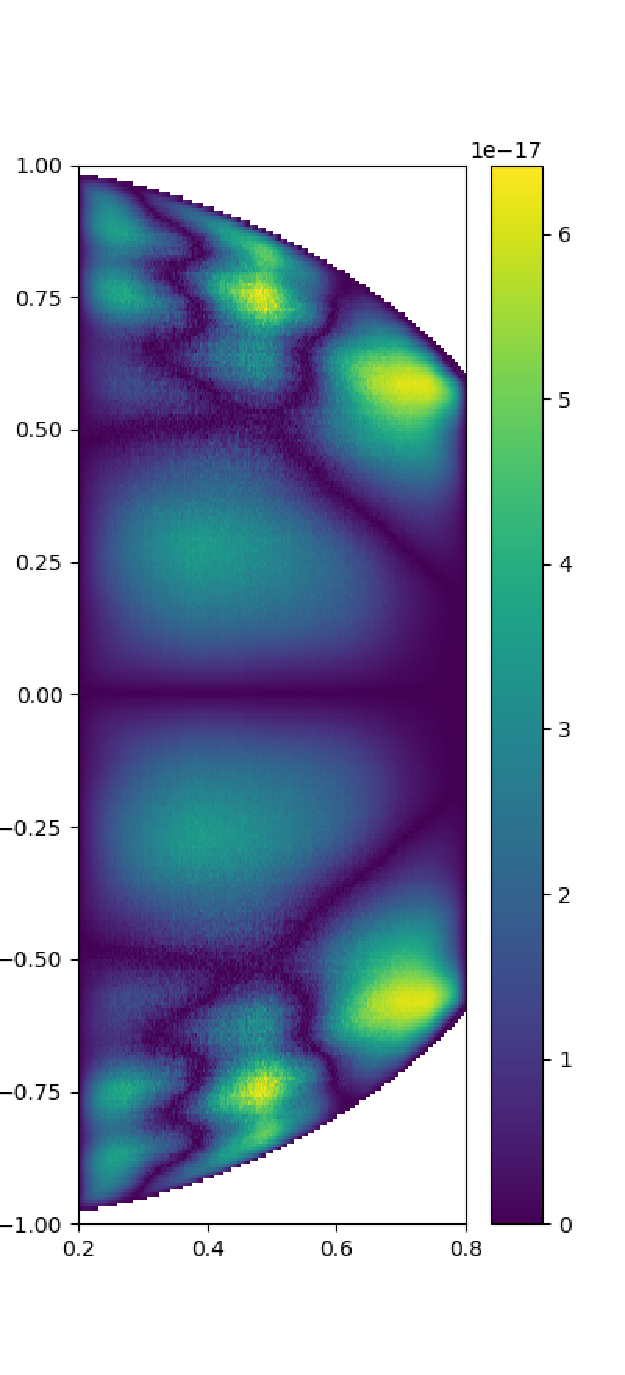
\includegraphics[scale=0.35]{solution-exact-poisson-diskslice-alpha=0p2-beta=0p8-u=y3expx-compare}
	\centering
	\end{subfigure}
	\centering
	\caption{The computed solution to $\Delta u = f$ with zero boundary conditions compared with the exact solution $u(x,y) = \Wiii (x,y) y^3 \exp(x)$. Left: Computed. Centre: Exact. Right: Plot of the error (colourbar is shown to demonstrate magnitude of the error is of the order $10^{-17}$)}
	\centering
	\label{fig:ds:poissonexact}
\end{figure}

\begin{figure}[t]
	\begin{subfigure}{0.3\textwidth}
	\centering
	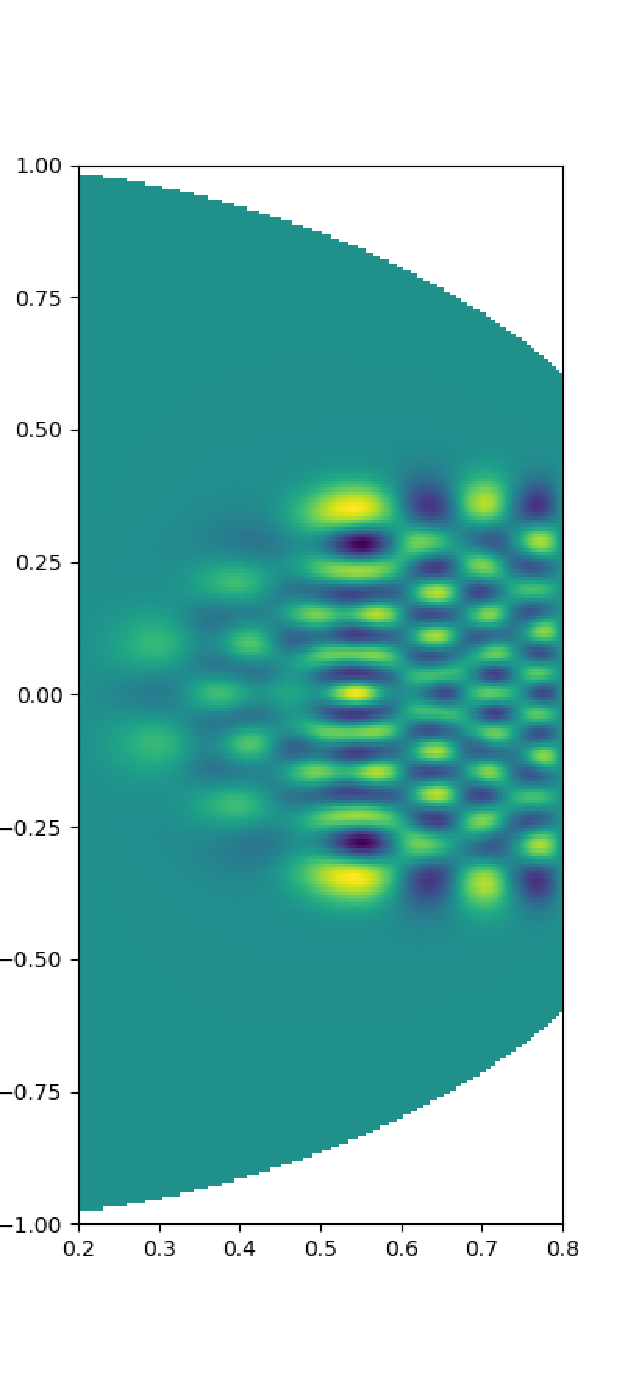
\includegraphics[scale=0.35]{solution-helmholtz-diskslice-alpha=0p2-beta=0p8-k=100-n=300}
	%\label{fig:ds:solution-helmholtz}
	\end{subfigure}
	\begin{subfigure}{0.5\textwidth}
	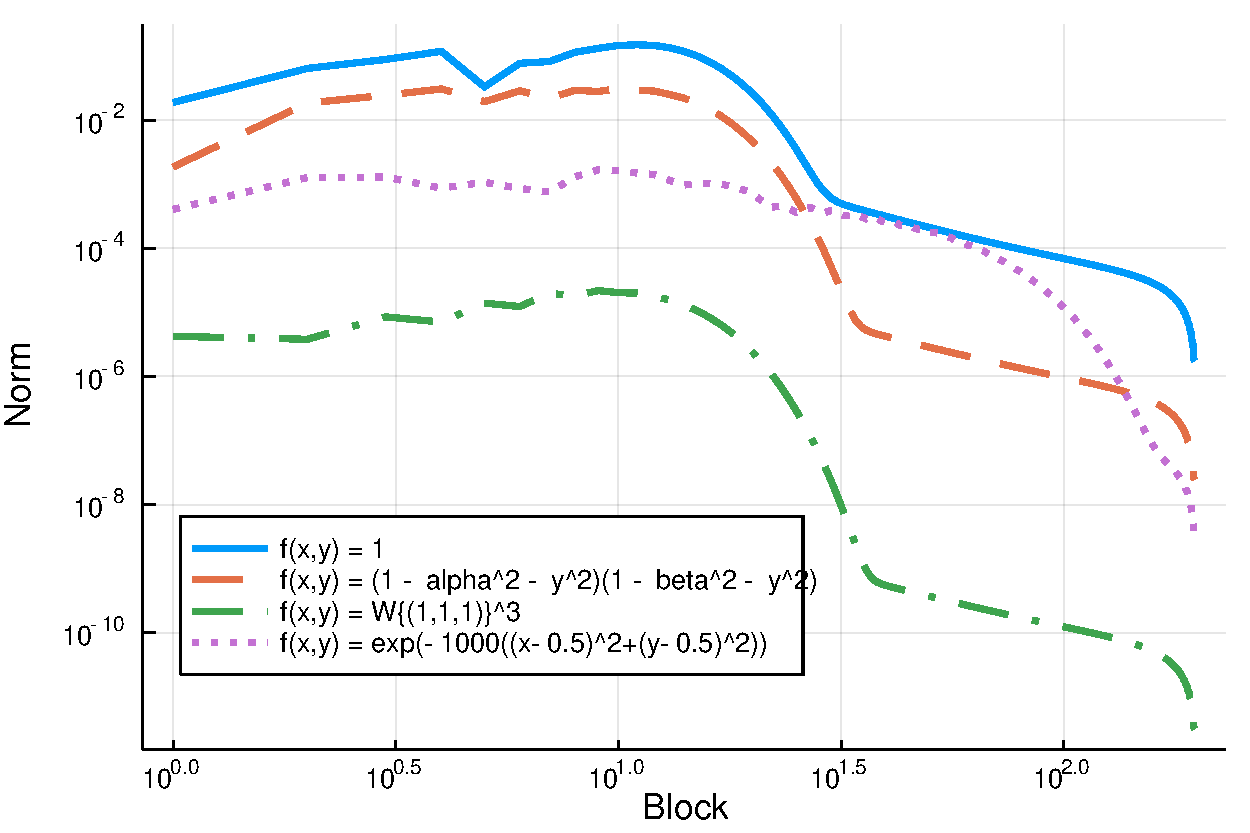
\includegraphics[scale=0.45]{solutionblocknorms-helmholtz-diskslice-alpha=0p2-beta=0p8-N=196-k=20}
	\centering
        	%\label{fig:ds:solutionblocknorms-helmholtz}
	\end{subfigure}
	\caption{Left: The computed solution to $\Delta u + k^2 \: v \: u = f$ with zero boundary conditions with $f(x,y) = x(1-x^2-y^2)e^x$, $v(x,y) = 1 - (3(x-1)^2 + 5y^2)$ and $k = 100$. Right: The norms of each block of the computed solution of the Helmholtz equation with the given right hand side functions, with $k=20$ and $v(x,y) = 1 - (3(x-1)^2 + 5y^2)$.}
	\centering
	\label{fig:ds:helmholtz}
\end{figure}

\begin{figure}[t]
	\begin{subfigure}{0.3\textwidth}
	\centering
	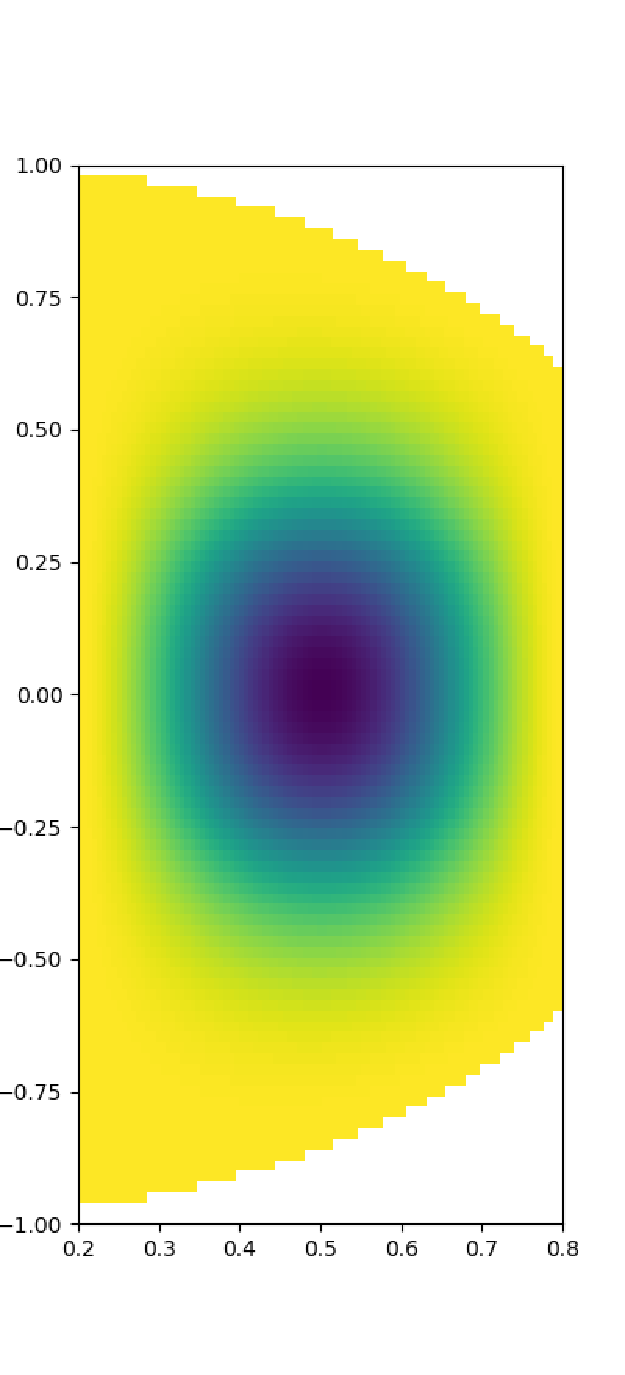
\includegraphics[scale=0.35]{solution-biharmonic-diskslice-alpha=0p2-beta=0p8}
	%\label{fig:ds:solution-biharmonic}
	\end{subfigure}
	\begin{subfigure}{0.5\textwidth}
	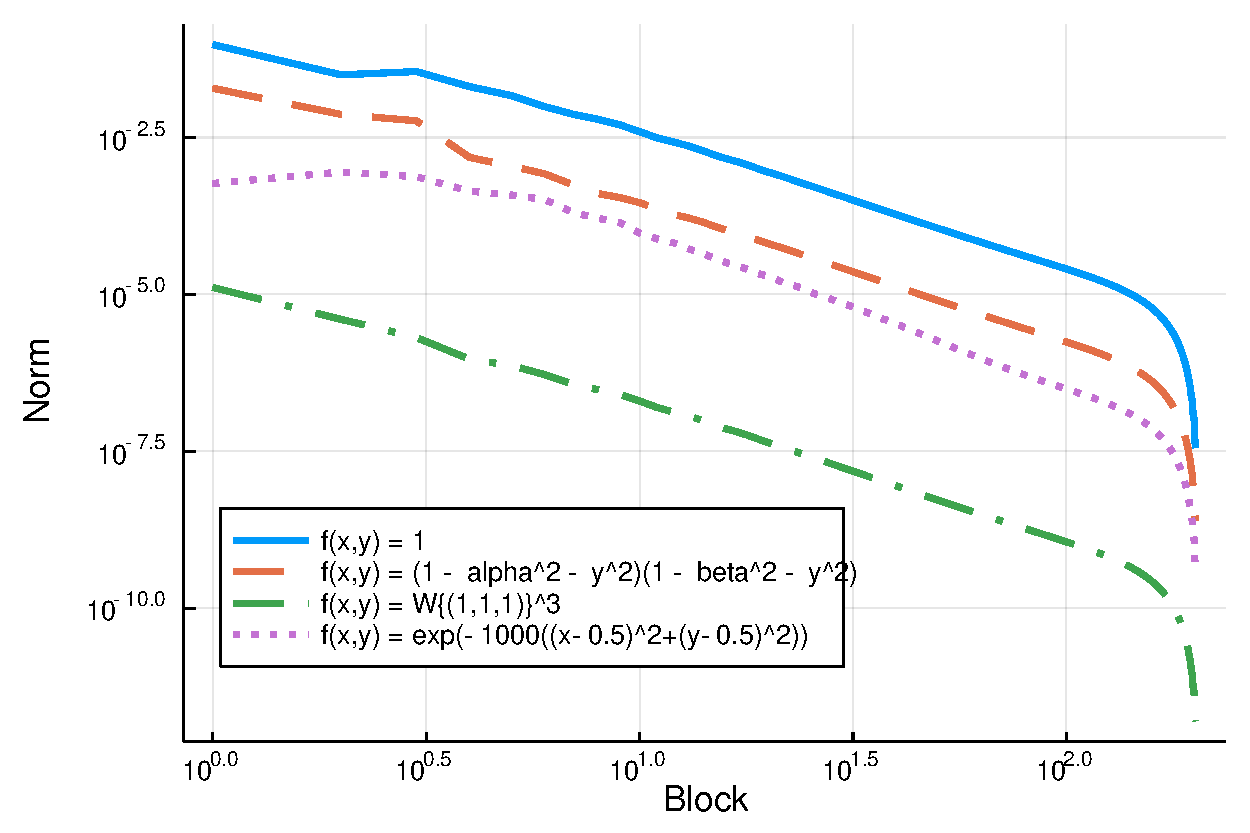
\includegraphics[scale=0.45]{solutionblocknorms-biharmonic-diskslice-alpha=0p2-beta=0p8-N=200}
	\centering
        	%\label{fig:ds:solutionblocknorms-biharmonic}
	\end{subfigure}
	\caption{Left: The computed solution to $\Delta^2 u = f$ with zero Dirichlet and Neumann boundary conditions with $f(x,y) = 1 + \text{erf}(5(1 - 10((x - 0.5)^2 + y^2)))$. Right: The norms of each block of the computed solution of the biharmonic equation with the given right hand side functions.}
	\centering
	\label{fig:ds:biharmonic}
\end{figure}
% END FIGURES

The Poisson equation is the classic problem of finding $u(x,y)$ given a function $f(x,y)$ such that:
\bseqnnumber{
	\begin{cases}
    		\Delta u(x,y) = f(x,y) \quad \text{in } \Omega \\
		u(x,y) = 0 \quad \text{on } \partial \Omega
	\end{cases}.
	\label{eqn:ds:poisson}
}
noting the imposition of zero Dirichlet boundary conditions on $u$.

We can tackle the problem as follows. Denote the coefficient vector for expansion of $u$ in the $\bigWiii$ OP basis up to degree $N$ by $\vec{u}$, and the coefficient vector for expansion of $f$ in the $\bighdopiii$ OP basis up to degree $N$ by $\vec{f}$. Since $f$ is known, we can obtain $\vec{f}$ using the quadrature rule above. In matrix-vector notation, our system hence becomes:
\bseqn{
    \laplacewiii \vec{u} = \vec{f}
}
which can be solved to find $\vec{u}$.
In \bsreffig{fig:ds:poisson} we see the solution to the Poisson equation with zero boundary conditions given in \bsrefeqn{eqn:ds:poisson} in the disk-slice $\Omega$. In \bsreffig{fig:ds:poisson} we also show the norms of each block of calculated coefficients of the approximation for four right-hand sides of the Poisson equation with $N = 990$, that is, $491,536$ unknowns. The rate of decay in the coefficients is a proxy for the rate of convergence of the computed solution: as typical of spectral methods, we expect the numerical scheme to converge at the same rate as the coefficients decay. We see that we achieve algebraic convergence for the first three examples, noting that for right hand-sides that vanish at the corners of our disk-slice ($x\in\{\alpha,\beta\}, \: y = \pm \rho(x)$) we observe faster convergence. 


In \bsreffig{fig:ds:poissonexact} we see an example where the solution calculated to the Poisson equation is shown together with a plot of the exact solution and the error. We see that the computed solution is almost exact. The example was chosen so that the exact solution was $u(x,y) = \Wiii (x,y) y^3 \exp(x)$, and thus the RHS function $f$ would be $f(x,y) = \Delta \big[ \Wiii(x,y) \: y^3 \: \exp(x) \big]$.


\subsection{Inhomogeneous variable-coefficient Helmholtz}

Find $u(x,y)$ given functions $v$, $f : \Omega \to \R$ such that:
\bseqnnumber{
	\begin{cases}
    		\Delta u(x,y) + k^2 \: v(x,y) \; u(x,y) = f(x,y) \quad \text{in } \Omega \\
		u(x,y) = 0 \quad \text{on } \partial \Omega
	\end{cases}.
	\label{eqn:ds:helmholtz}
}
where $k \in \R$, noting the imposition of zero Dirichlet boundary conditions on $u$.

We can tackle the problem as follows. Denote the coefficient vector for expansion of $u$ in the $\bigWiii$ OP basis up to degree $N$ by $\vec{u}$, and the coefficient vector for expansion of $f$ in the $\bighdopiii$ OP basis up to degree $N$ by $\vec{f}$. Since $f$ is known, we can obtain  the coefficients $\vec{f}$ using the quadrature rule above. We can obtain the matrix operator for the variable-coefficient function $v(x,y)$ by using the Clenshaw algorithm with matrix inputs as the Jacobi matrices ${J_x^{(0,0,0)}}^\top, {J_y^{(0,0,0)}}^\top$, yielding an operator matrix of the same dimension as the input Jacobi matrices a la the procedure introduced in \cite{olver2019triangle}. We can denote the resulting operator acting on coefficients in the $\bighdopooo$ space by $V({J_x^{(0,0,0)}}^\top, {J_y^{(0,0,0)}}^\top)$. In matrix-vector notation, our system hence becomes:
\bseqn{
    (\laplacewiii + k^2 T^{(0,0,0)\to(1,1,1)} \: V({J_x^{(0,0,0)}}^\top, {J_y^{(0,0,0)}}^\top) \: T_W^{(1,1,1)\to(0,0,0)}) \vec{u} = \vec{f}
}
which can be solved to find $\vec{u}$. We can see the sparsity and structure of this matrix system in \bsreffig{fig:ds:sparsity} with $v(x,y) = xy^2$ as an example. In \bsreffig{fig:ds:helmholtz} we see the solution to the inhomogeneous variable-coefficient Helmholtz equation with zero boundary conditions given in \bsrefeqn{eqn:ds:helmholtz} in the half-disk $\Omega$, with $k=100$, $v(x,y) = 1 - (3(x-1)^2 + 5y^2)$ and $f(x,y) = x(1-x^2-y^2)e^x$. In \bsreffig{fig:ds:helmholtz} we also show the norms of each block of calculated coefficients of the approximation for four right-hand sides of the inhomogeneous variable-coefficient Helmholtz equation with $k=20$ and $v(x,y) = 1 - (3(x-1)^2 + 5y^2)$ using $N = 500$, that is, $125,751$ unknowns. The rate of decay in the coefficients is a proxy for the rate of convergence of the computed solution. We see that we achieve algebraic convergence for the first three examples, noting that for right hand sides that vanish at the corners of our disk-slice ($x\in\{\alpha,\beta\}, \: y = \pm \rho(x)$) we see faster convergence.

% For the final Gaussian bump example, we see that we achieve spectral convergence.

We can extend this to constant non-zero boundary conditions by simply noting that the problem 
\bseqn{
	\begin{cases}
    		\Delta u(x,y) + k^2 \: v(x,y) \; u(x,y) = f(x,y) \quad \text{in } \Omega \\
		u(x,y) = c \in \R \quad \text{on } \partial \Omega
	\end{cases}
}
is equivalent to letting $u = \tilde{u} + c$ and solving
\bseqn{
	\begin{cases}
    		\Delta \tilde{u}(x,y) + k^2 \: v(x,y) \; \tilde{u}(x,y) = f(x,y) - c \: k^2 \: v(x,y) \; =: g(x,y)  \quad \text{in } \Omega \\
		\tilde{u}(x,y) = 0 \quad \text{on } \partial \Omega.
	\end{cases}.
}


\subsection{Biharmonic equation}

Find $u(x,y)$ given a function $f(x,y)$ such that:
\bseqnnumber{
	\begin{cases}
    		\Delta^2 u(x,y) = f(x,y) \quad \text{in } \Omega \\
		u(x,y) = 0, \quad \frac{\partial u}{\partial n}(x,y) = 0 \quad \text{on } \partial \Omega
	\end{cases}.
	\label{eqn:ds:biharmonic}
}
where $\Delta^2$ is the Biharmonic operator, noting the imposition of zero Dirichlet and Neumann boundary conditions on $u$. In \bsreffig{fig:ds:biharmonic} we see the solution to the Biharmonic \bsrefeqn{eqn:ds:biharmonic} in the disk-slice $\Omega$. In \bsreffig{fig:ds:biharmonic} we also show the norms of each block of calculated coefficients of the approximation for four right-hand sides of the biharmonic equation with $N = 500$, that is, $125,751$ unknowns.  We see that we achieve algebraic convergence for the first three examples, noting that for right hand sides that vanish at the corners of our disk-slice ($x\in\{\alpha,\beta\}, \: y = \pm \rho(x)$) we see faster convergence.


%%%%%
\section{Other domains}

\subsection{End-Disk-Slice}\label{section:ds:enddiskslice}

The work in this paper on the disk-slice can be easily transferred to the special-case domain of the end-disk-slice, such as half disks, by which we mean
\bseqn{
	\Omega := \{(x,y) \in \R^2 \quad | \quad \alpha < x < \beta, \: \gamma \rho(x) < y < \delta \rho(x)\}
}
with
\bseqn{
\begin{cases}
\alpha &\in (0,1) \\
\beta &:= 1 \\
(\gamma, \delta) &:= (-1,1) \\
\rho(x) &:= (1-x^2)^{\half}.
\end{cases}
}
Our 1D weight functions on the intervals $(\alpha, \beta)$ and $(\gamma, \delta)$ respectively are then given by:
\bseqn{
\begin{cases}
\genjacw^{(a,b)}(x) &:= (x - \alpha)^{a} \: \rho(x)^{b} \\
\jacw^{(a)}(x) &:= (1-x^2)^b.
\end{cases}
}

Note here how we can remove the need for third parameter, which is why we consider this a special case. This will make some calculations easier, and the operator matrices more sparse. The weight $\jacw^{(b)}(x)$ is a still the same ultraspherical weight (and the corresponding OPs are the Jacobi polynomials $\{\jac_n^{(b, b)}\}$). $\genjacw^{(a,b)}(x)$ is the (non-classical) weight for the OPs denoted $\{\genjac_n^{(a,b)}\}$. Thus we arrive at the two-parameter family of 2D orthogonal polynomials $\{\hdopnkab\}$ on $\Omega$ given by, for \(0 \le k \le n, \: n = 0,1,2,\dots,\)
\bseqn{
	\hdopnkab(x,y) := \genjacnmk^{(a, 2b+2k+1)}(x) \: \rho(x)^k \: \jac_k^{(b,b)}\fpr(\frac{y}{\rho(x)}), \quad (x,y) \in \Omega, 
}
orthogonal with respect to the weight
\bseqn{
	\Wab(x,y) &:= \genjacw^{(a,2b)}(x) w^{(b)}_P\fpr(\frac{y}{\rho(x)}) \nonumber \\
	&= (x - \alpha)^{a} \: (\rho(x)^2 -y^2)^b \nonumber \\
	&= (x - \alpha)^{a} \: (1 - x^2 -y^2)^b , \quad (x,y) \in \Omega.
}

The sparsity of operator matrices for partial differentiation by $x, y$ as well as for parameter transformations generalise to such end-disk-slice domains. For instance, if we inspect the proof of \bsreftheorem{theorem:ds:sparsityofdifferentialoperators}, we see that it can easily generalise to the weights and domain $\Omega$ for an end-disk-slice.

In \bsreffig{fig:ds:trappfem} we see the solution to the Poisson equation with zero boundary conditions in the half-disk $\Omega$ with $(\alpha,\beta) := (0,1)$.


\subsection{Trapeziums}\label{section:ds:trapezium}

We can further extend this work to trapezium shaped domains. Note that for any trapezium there exists an affine map to the canonical trapezium domain that we consider here, given by
\bseqn{
	\Omega := \{(x,y) \in \R^2 \quad | \quad \alpha < x < \beta, \: \gamma \rho(x) < y < \delta \rho(x)\}
}
with 
\bseqn{
\begin{cases}
(\alpha, \beta) &:= (0,1) \\
(\gamma, \delta) &:= (0,1) \\
\rho(x) &:= 1- \xi x, \quad \xi \in (0,1) \\
\genjacw^{(a,b,c)}(x) &:= (\beta - x)^a \: (x - \alpha)^{b} \: \rho(x)^{c} = (1-x)^{a} \: x^b \: (1-\xi x)^{c} \\
\jacw^{(a,b)}(x) &:= (\delta-x)^a \: (x - \gamma)^b = (1-x)^a \: x^b.
\end{cases}
}
The weight $\jacw^{(a,b)}(x)$ is the weight for the shifted Jacobi polynomials on the interval $[0,1]$, and hence the corresponding OPs are the shifted Jacobi polynomials $\{\tilde{P}_n^{(a, b)}\}$. We note that the shifted Jacobi polynomials relate to the normal Jacobi polynomials by the relationship $\tilde{P}_n^{(a,b)}(x) = \jac_n^{(a,b)}(2x-1)$ for any degree $n = 0,1,2,\dots$ and $x \in [0,1]$. $\genjacw^{(a,b,c)}(x)$ is the (non-classical) weight for the OPs we dentote $\{\genjac_n^{(a,b,c)}\}\). Thus we arrive at the four-parameter family of 2D orthogonal polynomials $\{\hdopnk^{(a,b,c,d)}\}$ on $\Omega$ given by, for \(0 \le k \le n, \: n = 0,1,2,\dots,\)
\bseqn{
	\hdopnk^{(a,b,c,d)}(x,y) := \genjacnmk^{(a, b, c+d+2k+1)}(x) \: \rho(x)^k \: \tilde{P}_k^{(d,c)}\fpr(\frac{y}{\rho(x)}), \quad (x,y) \in \Omega, 
}
orthogonal with respect to the weight
\bseqn{
	W^{(a,b,c,d)}(x,y) &:= \genjacw^{(a,b,c+d)}(x) \: w^{(d,c)}_P\fpr(\frac{y}{\rho(x)}) \nonumber \\
	&= (1-x)^a \: x^b \: y^c \: (1- \xi x - y)^d, \quad (x,y) \in \Omega.
}

In \bsreffig{fig:ds:trappfem} we see the solution to the Helmholtz equation with zero boundary conditions in the trapezium $\Omega$ with $\xi := \half$. 

%\subsection{Quadrature rule on the trapezium}
%
%In this section we construct a quadrature rule exact for polynomials in the trapezium $\Omega$ that can be used to expand functions in $\hdopnkabcd(x,y)$.
%
%\begin{theorem}
%Denote the Gauss quadrature nodes and weight on $[\alpha,\beta]$ with weight $\genjacw^{(a,b,c+d)}(s) = (\beta - s)^a \: (s - \alpha)^b \: \rho(s)^{c+d+1}$ as $(s_k,w_k^{(s)})$ , and
% on $[0,1]$ with weight $\jacw^{(d,c)}(t) = t^c \: (1-t)^d$ as $(t_k,w_k^{(t)})$. Define
%\bseqn{
%	x_{i+(j-1)N} &:= s_j, \quad i,j = 1,\dots, \ceil{\frac{N+1}{2}}, \\
%	y_{i+(j-1)N} &:= \rho(s_j) \: t_i, \quad i,j = 1,\dots, \ceil{\frac{N+1}{2}}, \\
%	w_{i+(j-1)N} &:= w_j^{(s)} w_i^{(t)}, \quad  i,j = 1,\dots, \ceil{\frac{N+1}{2}}.
%}
%Let $f(x,y)$ be a polynomial on $\Omega$. The quadrature rule is then
%$$
%\iint_\Omega f(x,y) \: \Wabcd(x,y) \: \D A \approx \sum_{j=1}^{M} w_j \: f(x_j, y_j)
%$$
%where $M = \ceil{\half(N+1)}^2$, and the quadrature rule is exact if $f(x,y)$ is a polynomial of degree $\le N$.
%\end{theorem}
%
%\begin{proof}
%\bseqn{
%	\iint_\Omega f(x,y) \: \Wabcd(x,y) \: \D y \: \D x &= \int_\alpha^\beta \genjacw^{(a,b,c+d+1)}(s) \: \Big( \int_{0}^{1} f\big(s,\rho(s) t\big) \: \jacw^{(d,c)}(t) \: \D t \Big) \: \D s \\
%	&\approx \int_\alpha^\beta \genjacw^{(a,b,c+d+1)}(s) \: \sum_{i=1}^{M_2} \Big( w_i^{(t)} f\big(s,\rho(s) t_i\big) \Big) \: \D s \quad (\star) \\
%	&\approx \sum_{j=1}^{M_1} \Bigg( w_j^{(s)} \: \sum_{i=1}^{M_2} \Big( w_i^{(t)} f\big(s_j,\rho(s_j) t_i\big) \Big) \Bigg) \quad (\star \star) \\
%	&= \sum_{k=1}^{M_1 M_2}  w_k \: f(x_k, y_k).
%}
%Suppose f is a polynomial in $x$ and $y$ of degree $N$. First, note that the degree of the polynomial given by $x \mapsto f(x,y)$ for fixed $y$ is $\le N$ and the degree of the polynomial given by $y \mapsto f(x,y)$ for fixed $x$ is $\le N$. Also note that $s \mapsto f\big(s,\rho(s) t\big)$ for fixed $t$ is then a degree $N$ polynomial (since $\rho$ is a degree $1$ polynomial). Hence, we achieve equality at $(\star)$ if $2M_2 - 1 \ge N$ and we achieve equality at $(\star \star)$ if also $2M_1 - 1 \ge N$.
%
%Thus, for a polynomial $f$ in $x$ and $y$ of degree $N$, 
%\bseqn{
%	\iint_\Omega f(x,y) \: \Wabcd(x,y) \: \D y \: \D x &= \int_\alpha^\beta \genjacw^{(a,b,c+d+1)}(s) \: \Big( \int_{0}^{1} f\big(s,\rho(s) t\big) \: \jacw^{(d,c)}(t) \: \D t \Big) \: \D s \\
%	&= \int_\alpha^\beta \genjacw^{(a,b,c+d+1)}(s) \: \sum_{i=1}^{\ceil{\half(N+1)}} \Big( w_i^{(t)} f\big(s,\rho(s) t_i\big) \Big) \: \D s \quad \\
%	&= \sum_{j=1}^{\ceil{\half(N+1)}} \Bigg( w_j^{(s)} \: \sum_{i=1}^{\ceil{\half(N+1)}} \Big( w_i^{(t)} f\big(s_j,\rho(s_j) t_i\big) \Big) \Bigg) \\
%	&= \sum_{k=1}^{M}  w_k \: f(x_k, y_k)
%}
%where $M = \ceil{\half(N+1)}^2$.
%
%\end{proof}


\section{P-finite element methods using sparse operators}\label{section:ds:PFEM}

\begin{figure}[t]
	\begin{subfigure}{0.3\textwidth}
	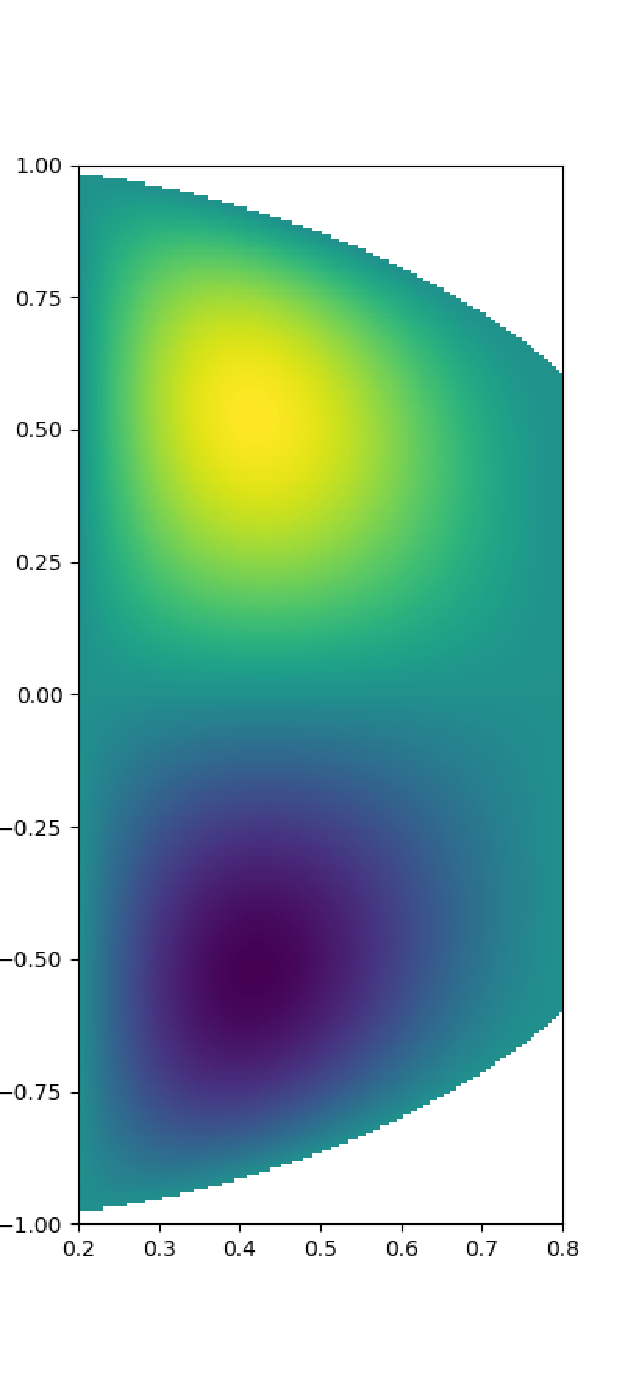
\includegraphics[scale=0.35]{solution-pfem-poisson-diskslice-alpha=0p2-beta=0p8-f=Wycosx}
        	%\label{fig:ds:solutionblocknorms-poisson}
	\centering
	\end{subfigure}
	\begin{subfigure}{0.3\textwidth}
	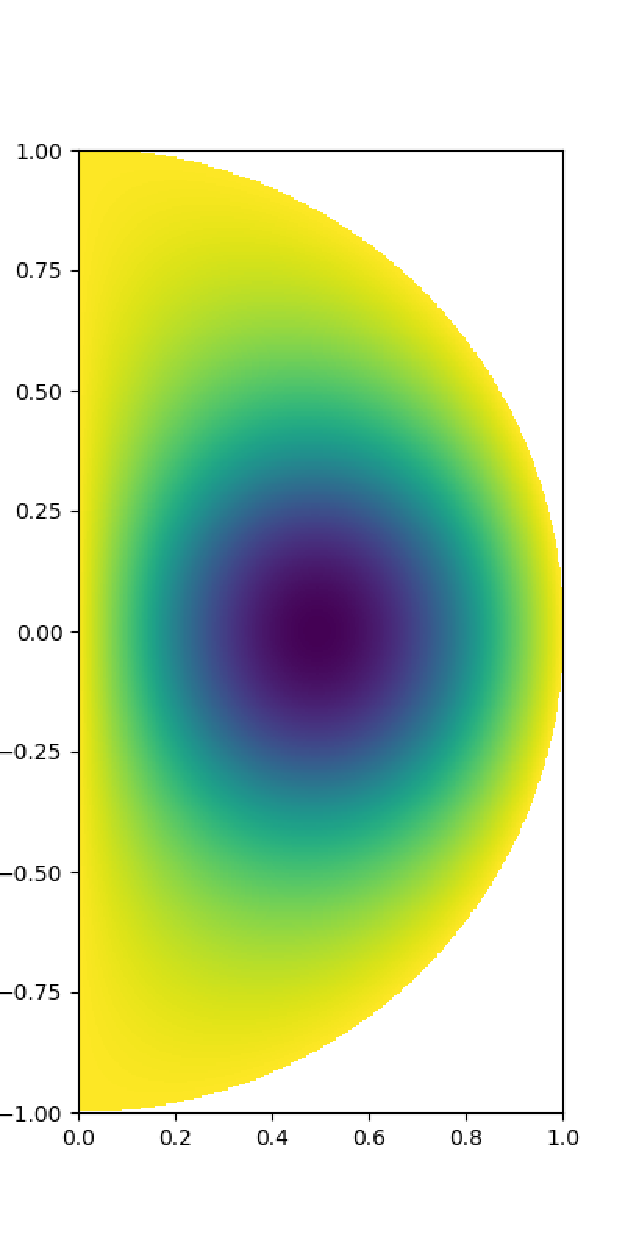
\includegraphics[scale=0.38]{solution-poisson}
	\centering
	%\label{fig:ds:solution-poisson}
	\end{subfigure}
	\begin{subfigure}{0.3\textwidth}
	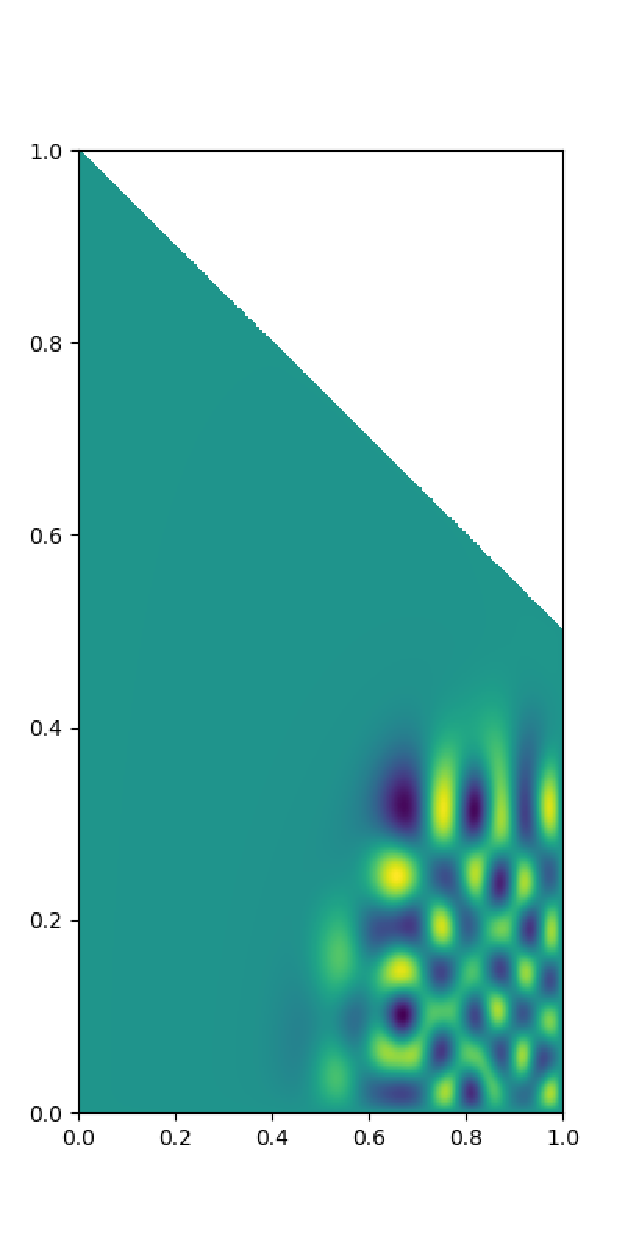
\includegraphics[scale=0.38]{solution-trapezium-helmholtz-k=100-n=1500}
	%\label{fig:ds:solution-poisson}
	\centering
	\end{subfigure}
	\centering
	\caption{Left: The computed solution to $\Delta u = f$ with zero boundary conditions with $f(x,y) = \Wiii(x,y) y \cos(x)$ in the disk-slice using the $p$-FEM approach with a single element. Centre: The computed solution to $\Delta u = f$ with zero boundary conditions with $f(x,y) = 1 + \text{erf}(5(1 - 10((x - 0.5)^2 + y^2)))$ in the half-disk. Right: The computed solution to $\Delta u + k^2 \: v \: u = f$ with zero boundary conditions with $f(x,y) = (1-x) \: x \: y \: (1- \half x - y) \: e^x$, $v(x,y) = 1 - (3(x-1)^2 + 5y^2)$ and $k = 100$. in the trapezium.}
	\centering
	\label{fig:ds:trappfem}
\end{figure}

It is possible for our framework to be applied to a $p$-finite element method -- that is, one where we can vary the polynomial degree $p$ of the basis functions used in each element (compare this to a normal $h$-FEM, where we can tune the element size $h$). For example, one could discretise the disk into disk-slice elements, and apply a $p$-finite element method to solve PDEs on the disk. As a precursor to this, in this section we limit our discretisation to a single element. Specifically, we follow the method of \cite{beuchler2006new} to construct a sparse $p$-finite element method in terms of the operators constructed above, with the benefit of ensuring that the resulting discretisation is symmetric. Consider the 2D Dirichlet problem on a domain $\Omega$:
\bseqn{
	\begin{cases}
         - \Delta u(x,y) = f(x,y) \quad \text{in } \Omega \\
         u = 0 \quad \text{on } \partial \Omega
         \end{cases}
}
This has the weak formulation for any test function $v \in V := H_0^1(\Omega) = \{v \in H^1(\Omega) \quad | \quad v|_{\partial \Omega} = 0 \}$,
\bseqn{
	L(v) := \int_\Omega f \: v \: \D \vec{x} = \int_\Omega \nabla u \cdot \nabla v \: \D \vec{x} =: a(u,v).
}

As eluded to, in general we would let $\FEset$ be the set of elements $\element$ that make up our finite element discretisation of the domain, where each $\element$ is a trapezium or disk slice for example. However, here we simply consider our domain to be a disk-slice and our discretisation to be a single element -- that is we let $\element = \Omega$ for a disk-slice domain. We can choose our finite dimensional space $V_p = \bsset{v_p \in V}{\deg(v_p|_\element) \le p}$ for some $p \in \N$.

We seek $u_p \in V_p$ s.t.
\bseqnnumber{
	L(v_p) = a(u_p,v_p) \quad \forall \: v_p \in V_p.
	\label{eqn:ds:FEMweakform}
}

Recall that the OPs $\bighdop^{(a,b,c)}$ are orthogonal with respect to the weight $\Wabc$ on $\Omega$, and define the matrix $\Lambda^{(a,b,c)} :=  \ip< \bighdop^{(a,b,c)}, \: {\bighdop^{(a,b,c)}}^\top >_{\Wabc}$. Note that due to orthogonality this is a diagonal matrix. We can choose a basis for $V_p$ by using the weighted orthogonal polynomials on $\element$ with parameters $a = b = c = 1$
\bseqn{
	\bigWiii(x,y) = \Wiii(x,y) \: \bighdopiii(x,y)
}
and rewrite \bsrefeqn{eqn:ds:FEMweakform} in matrix form:
\bseqn{
	&a(u_p,v_p) \\
	&= \int_\element \begin{pmatrix}
					\partial_x v_p \\
					\partial_y v_p
				\end{pmatrix}^\top 
				\begin{pmatrix}
					\partial_x u_p \\
					\partial_y u_p
				\end{pmatrix} \: \D \vec{x}
				\\
	&= \int_\element \begin{pmatrix}
					\bighdopooo^\top \Wiii_x \vec{v} \\
					\bighdopooo^\top T_W^{(1,1,0)\to(0,0,0)} \Wiii_y \vec{v}
				\end{pmatrix}^\top 
				\begin{pmatrix}
					\bighdopooo^\top \Wiii_x \vec{u} \\
					\bighdopooo^\top T_W^{(1,1,0)\to(0,0,0)} \Wiii_y \vec{u}
				\end{pmatrix} \: \D \vec{x}
				\\
	&= \int_\element \Big( \vec{v}^\top {\Wiii_x}^\top \bighdopooo \bighdopooo^\top \Wiii_x \vec{u} \nonumber \\
					& \quad \quad \quad + \vec{v}^\top ({T_W^{(1,1,0)\to(0,0,0)} \Wiii_y})^\top \bighdopooo \bighdopooo^\top T_W^{(1,1,0)\to(0,0,0)} \Wiii_y \vec{u}  \Big) \: \D \vec{x} \\
	&= \vec{v}^\top \: \Big( {\Wiii_x}^\top \Lambda^{(0,0,0)} \Wiii_x \\
	& \quad \quad \quad \quad + ({T_W^{(1,1,0)\to(0,0,0)} \Wiii_y})^\top \Lambda^{(0,0,0)} T_W^{(1,1,0)\to(0,0,0)} \Wiii_y \Big) \: \vec{u}
}
where $\vec{u}, \vec{v}$ are the coefficient vectors of the expansions of $u_p, v_p \in V_p$ respectively in the $V_p$ basis ($\bigWiii$ OPs), and
\bseqn{
	L(v_p) &= \int_\element \: v_p \: f \: \D \vec{x}\\
	&= \int_\element \: \vec{v}^\top \: \bigWiii \: \bighdopiii^\top \: \vec{f} \: \D \vec{x} \\
	&= \vec{v}^\top \: \ip< \bighdopiii, {\bighdopiii}^\top >_{\Wiii} \: \D \vec{x} \\
	&= \vec{v}^\top \Lambda^{(1,1,1)} \: \vec{f},
}
where $\vec{f}$ is the coefficient vector for the expansion of the function $f(x,y)$ in the $\bighdopiii$ OP basis.

Since \bsrefeqn{eqn:ds:FEMweakform} is equivalent to stating that
\bseqn{
	L(\Wiii \hdopiii_{n,k}) = a(u_p,\Wiii \hdopiii_{n,k}) \quad \forall \: n = 0,\dots,p, \: k = 0,\dots,n,
}
(i.e. holds for all basis functions of $V_p$) by choosing $v_p$ as each basis function, we can equivalently write the linear system for our finite element problem as:
\bseqn{
	A\vec{u} = \tilde{\vec{f}}.
}
where the (element) stiffness matrix $A$ is defined by 
\bseqn{
	A = {\Wiii_x}^\top \Lambda^{(0,0,0)} \Wiii_x + ({T_W^{(1,1,0)\to(0,0,0)} \Wiii_y})^\top \Lambda^{(0,0,0)} T_W^{(1,1,0)\to(0,0,0)} \Wiii_y
}
and the load vector $\tilde{\vec{f}}$ is given by 
\bseqn{
	\tilde{\vec{f}} = \Lambda^{(1,1,1)} \: \vec{f}.
}

Note that since we have sparse operator matrices for partial derivatives and basis-transform, we obtain a symmetric sparse (element) stiffness matrix, as well as a sparse operator matrix for calculating the load vector (rhs).



\section{Conclusions}

In this chapter we have shown that bivariate orthogonal polynomials can lead to sparse discretizations of general linear PDEs on specific domains whose boundary is specified by an algebraic curve -- notably here the disk-slice -- with Dirichlet boundary conditions. This work extends the triangle case \cite{beuchler2006new, li2010optimal, olver2019triangle} and whole disk case \cite{boyd2011comparing, vasil2016tensor} to non-classical geometries, and forms a building block in developing an $hp-$finite element method to solve PDEs on other polygonal domains by using suitably shaped elements (for example, by dividing the disk or a section of the disk into disk-slice elements, which has applications in turbulent pipe flow \cite{eggels1994fully, kerswell2005recent, vasil2016tensor}).

We have demonstrated how one can construct the three-or-four-parameter OP families (depending on the domain) that form the basis for our sparse spectral methods, and presented a procedure, utilising the Christoffel-Darboux formula \cite[18.2.2]{DLMF}, of explicitly calculating the recurrence coefficients for the univariate OPs that are part of the construction. These coefficients contribute to calculations of the entries in the Jacobi matrices and other differential operators. Moreover, we have defined a quadrature rule that can be used for expanding functions in our OP basis and for calculating said entries of important operators. We have looked at a few mathematical examples including the Poisson, variable coefficient Helmholtz, and biharmonic equations and shown that our method performs well. Importantly, all operator matrices used are shown to be sparse, and in fact banded-block-banded in structure.

Looking ahead, this work serves as a stepping stone to constructing similar methods to solve partial differential equations on sub-domains of the $2$-sphere surface, such as spherical caps that we will discuss in the next chapter.


%, see \cite[Theorem 3.1]{olver2018orthogonal} for a similar construction of OPs on an arc in 2D, and it is clear from the construction in this paper that discretizations of spherical gradients and Laplacian's are sparse on half-spheres and other suitable sub-components of the sphere. The resulting sparsity in high-polynomial degree discretizations presents an attractive alternative to methods based on bijective mappings (e.g., \cite{DGShallowWater,FEMShallowWater,boyd2005sphere}). Constructing these sparse spectral methods for surface PDEs on half-spheres, spherical caps, and spherical triangles is future work, and has applications in weather prediction \cite{staniforth2012horizontal}. Other extensions include a full $hp$-finite element method on sections of a disk, which has applications in turbulent pipe flow.









  


\chapter{Spherical caps}\label{CHAPTER:sphericalcaps}

While the work in the previous chapter looked at developing a sparse spectral method inside a two dimensional domain, we move on to investigating the realm of a surface in three dimensional space. Specifically, we look to extend the methodology to a hierarchy of non-classical multivariate orthogonal polynomials on spherical caps. The entries of discretisations of partial differential operators can be effectively computed using formulae in terms of (non-classical) univariate orthogonal polynomials. We demonstrate the results on partial differential equations involving the spherical Laplacian and biharmonic operators, showing spectral convergence with discretisations that can be made well-conditioned using a simple preconditioner. 

Our aim in this chapter is to develop a sparse spectral method for solving linear partial differential equations on certain subsets of the sphere -- specifically spherical caps. More precisely, we consider the solution of partial differential equations on the \textit{spherical cap} $\Omega$ defined by
\bseqn{
	\Omega := \bsset{(x,y,z) \in \R^3}{\alpha < z < \beta, \: x^2 + y^2 + z^2 = 1}
}
where $\alpha \in (-1,1)$ and $\beta := 1$. Simply put, the region of the surface of the $2$-sphere where the $z$-coordinate range is limited to a sub-interval of $[-1,1]$ is what we refer to as the spherical cap.

\begin{remark}
For simplicity we focus on the case of a spherical cap, though there is an extension to a spherical band by taking $\beta \in (\alpha,1)$. The methods presented here translate to the spherical band case by including the necessary adjustments to the weights and recurrence relations we present in this paper. These adjustments make the construction more involved, but the approach is essentially the same which is why they are omitted here.
\end{remark}

For the spherical cap, we advocate using a basis that is polynomial in cartesian coordinates, that is, polynomial in $x$, $y$, and $z$, and orthogonal with respect to a prescribed weight: that is, multivariate orthogonal polynomials, whose construction was considered in \cite{olver2020orthogonal}. Equivalently, we can think of these as polynomials modulo the vanishing ideal $\bsset{(x,y,z) \in \R^3}{x^2 + y^2 + z^2 = 1}$, or simply as a linear recombination of spherical harmonics that are orthogonalised on a subset of the sphere. This is in contrast to more standard approaches based on mapping the geometry to a simpler one (e.g., a rectangle or disk) and using orthogonal polynomials in the mapped coordinates (e.g., a basis that is polynomial in the spherical coordinates $\varphi$ and $\theta$). The benefit of the new approach is that we do not need to resolve Jacobians, and thereby we can achieve sparse discretisations for partial differential operators, including those with polynomial variable coefficients. Further, we avoid the singular nature at the poles or as $\alpha$ approaches $0$ that such a projection may give, since our new approach yields a smooth polynomial basis for all $\alpha \in [-1,1)$. 

There are of course other approaches for solving PDEs on surfaces, such as the closest point method \cite{macdonald2010implicit, macdonald2008level}. This involves recasting the PDE as one involving a \enquote{closest point} operator in a 3D volume that acts as a \enquote{shell} for the surface. While such an approach is useful for other geometries, it is of low order and does not achieve spectral convergence with sparse discretisations. Further, for our domain of interest, the closest point method does not take advantage of any rotational symmetry, and so is unable to achieve optimal complexity with a direct solver.

On the spherical cap, the family of weights we will consider are of the form
\bseqn{
	\Wa(x,y,z) := (z - \alpha)^a, \qfor (x,y,z) \in \Omega,
}
noting that $\Wa(x,y,z) = 0$ for $(x,y,z) \in \partial \Omega$ when $a > 0$. The corresponding OPs denoted $\scopnkia(x,y,z)$, where $n$ denotes the polynomial degree, $0 \le k \le n$ and $i \in \{0, \min(1,k)\}$. We define these to be orthogonalised lexicographically, that is,
\bseqn{
	\scopnkia(x,y,z) = C_{n,k,i} \: x^{k-i} \: y^i \: z^{n-k} + (\hbox{lower order terms})
}
where $C_{n,k,i} \neq 0$ and \enquote{lower order terms} includes degree $n$ polynomials of the form $x^{j - i} \: y^{i} \: z^{n-j}$ where $j < k$. The precise normalization arises from their definition in terms of one-dimensional OPs that we will see in \bsrefdef{def:sc:OPconstruction}. 

Just as for the spherical harmonics framework for the whole sphere in \bsrefchapter{CHAPTER:sphericalharmonics}, we consider partial differential operators involving the spherical Laplacian (the Laplace--Beltrami operator). Recall that we write the spherical coordinates as
\bseqn{
	x &= \sinphi \costheta = \rho(z) \costheta \\
	y &= \sinphi \sintheta = \rho(z) \sintheta \\
	z &= \cosphi
}
where $ \rho(z) := \sqrt{1-z^2}$, and that the Laplace--Beltrami operator is then
\bseqn{
	\DeltaS &= {1 \over \sinphi} \ppphi \Big( \sinphi \ppphi \Big) + {1 \over \sin^2 \varphi} \ppthetatwo = {1 \over \rho} \ppphi \Big( \rho \ppphi \Big) + {1 \over \rho^2} \ppthetatwo
}
i.e. $\DeltaS f(\xvec) = \Delta f({\xvec \over \norm{\xvec}})$ for $\xvec := (x,y,z) \in \R^3$. We do so by considering the component operators $\rho {\partial \over \partial \varphi}$ and ${\partial \over \partial \theta}$ applied to OPs with a specific choices of weight so that their discretisation is sparse, see \bsreftheorem{theorem:sc:sparsityofdifferentialoperators}. Sparsity comes from expanding the domain and range of an operator using different choices of the parameter $a$, a la the ultraspherical spectral method we investigated in \bsrefchapter{CHAPTER:diskslice} for disk-slices and trapeziums (see also \cite{snowball2019sparse}), as well as for intervals \cite{olver2013fast}, triangles \cite{olver2019triangle}, and the related work on sparse discretisations involving Jacobi polynomials on disks \cite{vasil2016tensor} and spheres \cite{vasil2019tensor,lecoanet2019tensor}. Just as we proceeded in \bsrefchapter{CHAPTER:diskslice} for the disk-slice case in 2D (see also \cite{snowball2019sparse}), we will use an integration-by-parts argument to deduce the sparsity structure.

The three-dimensional orthogonal polynomials defined here involve the same non-classical (in fact, semi-classical \cite[\S5]{magnus1995painleve}) 1D OPs as those outlined for the disk-slice, and so methods for calculating these 1D OP recurrence coefficients and integrals have already been outlined in \bsrefchapter{CHAPTER:diskslice} (see also \cite{snowball2019sparse}). In particular, by exploiting the connection with these 1D OPs we can construct discretizations of general partial differential operators of size $(p+1)^2 \times (p+1)^2$ in $O(p^3)$ operations, where $p$ is the total polynomial degree. This clearly compares favourably to proceeding in a na\"ive approach where one would require $O(p^6)$ operations.

Note that we consider partial differential operators that are not necessarily rotational invariant: for example, one can use these techniques for Schr\"odinger operators $\DeltaS + v(x,y,z)$ where $v$ is first approximated by a polynomial. A nice feature is that if the partial differential operator is invariant with respect to rotation around the $z$ axis (e.g., a Schr\"odinger operator with potential $v(z)$) the discretisation decouples, and can be reordered as a block-diagonal matrix. This improves the complexity further to an optimal $O(p^2$), which is demonstrated in \bsreffig{fig:sc:complexity} with $v(x,y,z) = \cos z$.

The code that allows one to produce the numerical examples in this chapter is publicly available as a Julia package\footnote{https://github.com/snowball13/OrthogonalPolynomialFamilies.jl} to partner the ApproxFun package \cite{ApproxFun} -- however, this package is purely experimental at this stage.




\section{The circle arc}\label{section:sc:arc}

The spherical cap can be thought of as a higher dimensional version of the circle arc (a one-dimensional \enquote{surface} in two-dimensional space). Recently, a procedure for defining OPs in two variables on quadratic curves, such as ellipses and parabolas, has been presented \cite{olver2021orthogonal}, where the unit circle is one of the five classes of curve that can be generalised to give any curve in the plane $\R^2$. One can define OPs on the circle in terms of Fourier series, which we write here as orthogonal polynomials in $x$ and $y$:
\begin{definition}[\cite{olver2021orthogonal}]\label{def:sc:Ydefinition}
	Define the unit circle $\omega := \bsset{\vec{x} = (x,y) \in \R^2}{x^2 + y^2 = 1}$, and define the parameter $\theta$ for each $(x,y) \in \omega$ by $x = \cos\theta$, $y = \sin\theta$. Define the polynomials $\{\chki\}$ for $k = 0, 1, \dots$, $i = 0, 1$ on $(x,y) \in \omega$ by
\bseqn{
	\ch_{0,0}(\xvec) \equiv \ch_{0,0}(x, y) &:= \ch_{0} =: \ch_{0,0}(\theta) \\
	\ch_{k,0}(\xvec) \equiv \ch_{k,0}(x, y) &:= T_k(x) = \cos k \theta =: \ch_{k,0}(\theta) \\
	\ch_{k,1}(\xvec) \equiv \ch_{k,1}(x, y) &:= y \: U_{k-1}(x) = \sin k \theta =: \ch_{k,1}(\theta)
}
for $k = 1,2,3,\dots$ where $\ch_{0} := {\sqrt{2} \over 2}$ and $T_k$, $U_{k-1}$ are the standard Chebyshev polynomials on the interval $[-1,1]$. The $\{Y_{k,i}\}$ are orthonormal with respect to the inner product
\bseqn{
	\ip< p, \: q >_{\ch} &:= \frac{1}{\pi} \: \int_0^{2\pi} p(\xvec(\theta)) \: q(\xvec(\theta)) \: \D \theta.
}
Note that $\ch_0$ is defined so as to ensure orthonormality. 
\end{definition}

However, for an arc of the unit circle $\bsset{\vec{x} = (x,y) \in \R^2}{x \ge h, \: x^2 + y^2 = 1}$ for some $h \in (-1, 1)$ (note we can orientate the arc as we please without loss of generality), we would need to make a modification so that the polynomials are orthonormal with respect to a different inner product accounting for the truncated domain of the arc:
\bseqn{
	\ip< p, \: q >_{\ch^h} &:= c^h \: \int_{-\arccos{h}}^{\arccos{h}} p(\xvec(\theta)) \: q(\xvec(\theta)) \: \D \theta \\
	&= c^h \: \int_h^1 \Big\{ p(x,\sqrt{1-x^2}) \; q(x,\sqrt{1-x^2}) \\
	&\quadfour \quadtwo + p(x,-\sqrt{1-x^2}) \; q(x,-\sqrt{1-x^2}) \Big\} {\D x \over \sqrt{1-x^2}}
}
for some normalising constant $c^h$. In the same vein, we can choose to construct the arc OPs in the same way as the whole circle OPs -- that is, define $\{T_k^h\}$, $\{U_k^h\}$ as two sets of univariate orthogonal polynomials on the interval $[h,1]$, orthogonal with respect to the weight functions $(1-x^2)^{-\half}$ and $(1-x^2)^{\half}$ respectively, and then define
\bseqn{
	\ch^h_{0,0}(\xvec) \equiv \ch^h_{0,0}(x, y) &:= \ch^h_{0} =: \ch^h_{0,0}(\theta) \\
	\ch^h_{k,0}(\xvec) \equiv \ch^h_{k,0}(x, y) &:= T^h_k(x) =: \ch^h_{k,0}(\theta) \\
	\ch^h_{k,1}(\xvec) \equiv \ch^h_{k,1}(x, y) &:= y \: U^h_{k-1}(x) =: \ch^h_{k,1}(\theta)
}
where $Y_0^h$ is chosen so that $\ip< Y_0^h, \: Y_0^h >_{\ch^h} = 1$.



\section{Orthogonal polynomials on spherical caps}\label{section:sc:OPs}

\subsection{Explicit construction}

A continuation to the procedure for defining OPs on quadratic curves (see \cite{olver2021orthogonal}) has also been presented \cite{olver2020orthogonal}, where OPs are defined on quadratic surfaces of revolution in higher dimensions (specifically, surfaces in $\R^{d+1} for d \ge 2$). The authors describe their technique as modelled on the structure of the unit sphere, by approaching the construction as a generalisation of spherical harmonics.

Using this approach, we can construct the 3D orthogonal polynomials on the spherical cap or band $\Omega$ from 1D orthogonal polynomials on the interval $[\alpha,\beta]$, and from Fourier series written as orthogonal polynomials in $x$ and $y$. Recall that the spherical cap is defined by
\bseqn{
	\Omega := \bsset{(x,y,z) \in \R^3}{\alpha < z < \beta, \: x^2 + y^2 + z^2 = 1}.
}
\begin{proposition}[\cite{olver2020orthogonal}]\label{prop:sc:OPconstruction}
	Let $w : (\alpha,\beta) \to \R$ be a weight function. For $n = 0,1,2,\dots, $ let $\{r_{n,k}\}$ be polynomials orthogonal with respect to the weight $\rho(x)^{2k} w(x)$ where $0 \le k \le n$. Then the 3D polynomials defined on $\Omega$ given by
\bseqn{
	\scopnki(x,y,z) := r_{n-k,k}(z) \: \rho(z)^k \: \ch_{k,i}\fpr({x \over \rho(z)}, {y \over \rho(z)})
}
for $i \in {0,1}, \: 0 \le k \le n, \: n = 0,1,2,\dots$ are orthogonal polynomials with respect to the inner product
\bseqn{
	&\ip< p, \: q > := \int_\Omega p(x,y,z) \: q(x,y,z) \: w(z) \: \D A \\
	&= \int_0^{\cos^{-1}(\alpha)} \int_0^{2\pi} \Big\{ p\big(\sinphi \costheta, \sinphi \sintheta, \cosphi \big) \: q\big(\sinphi \costheta, \sinphi \sintheta, \cosphi \big) \\
	&\quadeight \quad \cdot w(\cosphi) \: \sinphi \Big\} \: \D \theta \: \D \varphi \\
	&= \int_\alpha^1 \int_0^{2\pi} p\big(\rho(z) \costheta, \rho(z) \sintheta, z\big) \: q\big(\rho(z) \costheta, \rho(z) \sintheta, z\big) \: w(z) \: \D \theta \: \D z
}
on $\Omega$, where $\D A = \sinphi \: \D \theta \: \D \varphi$ is the uniform spherical measure on $\Omega$. 
\end{proposition}

For the spherical cap, we can use \bsrefprop{prop:sc:OPconstruction} to create our one-parameter family of OPs. The univariate OPs that we will choose for the $r_{n,k}$ polynomials above will be the non-classical $\genjac^{(a,b)}$ OPs that we defined in \bsrefdef{def:ds:OPconstruction}. Since there is only one boundary for the spherical cap, we will only need to use a two-parameter version\footnote{For a spherical band with two boundaries, we would need the three-parameter version}). For reference, the family of orthonormal polynomials on $[\alpha,\beta]$ denoted $\{\genjac_n^{(a,b)}\}$ are defined such that they are orthonormal with respect to the inner product
\bseqnnumber{
	\ip< p, \: q >_{\genjacw^{(a,b)}} &:= \frac{1}{\normgenjac^{(a,b)}} \: \int_\alpha^1 p(x) \: q(x) \: \genjacw^{(a,b)}(x) \: \D x \label{eqn:sc:ipgenjac}
}
where
\bseqn{
	\genjacw^{(a,b)}(x) &:= (x - \alpha)^{a} \: \rho(x)^{b}
} is the weight function and 
\bseqnnumber{
	\normgenjac^{(a,b)} := \int_\alpha^1 \: \genjacw^{(a,b)}(x) \: \D x \label{eqn:sc:ipnormalisation}
}
is a normalising constant.

We can now define the 3D OPs for the spherical cap.
\begin{definition}\label{def:sc:OPconstruction}
	Define the one-parameter 3D orthogonal polynomials via:
\bseqnnumber{
	\scopnkia(x,y,z) := \genjacnmk^{(a,2k)}(z) \: \rho(z)^k \: \chki\fpr(\frac{x}{\rho(z)}, \frac{y}{\rho(z)}), \quad (x,y,z) \in \Omega.
}
\end{definition}

By construction, $\{\scopnkia\}$ are orthogonal with respect to the inner product \nomenclature[innerQ]{$\ip< p, \: q >_{\scopa}$}{A multidimensional inner product over $\Omega$ with the weight $\Wa$ associated with the OPs $\{\scopnkia\}$}
\bseqn{
	\ip< p, \: q >_{\scopa} &:= \int_\Omega p(\xvec, z) \: q(\xvec, z) \: \genjacw^{(a,0)}(z) \: \D A \\
	&= \int_\alpha^1 \int_0^{2\pi} p(\rho(z) \cos\theta, \rho(z) \sin\theta, z) \: q(\rho(z) \cos\theta, \rho(z) \sin\theta, z) \: \D \theta \: \genjacw^{(a,0)}(z) \: \D z,
}
with \nomenclature[normQ]{$\norm{f}_{\scopa}$}{The norm of a function f, defined by the square root of the inner product over $\Omega$ given by the weight $\Wa$ associated with the OPs $\{\scopnkia\}$}
\bseqnnumber{
	\norm{\scopnkia}_{\scopa}^2 &:= \ip< \scopnkia, \: \scopnkia >_{\scopa} = \pi \: \normgenjac^{(a, 2k)}. \label{eqn:sc:normscop}
}
A method for obtaining explicit recurrence coefficients and evaluating integrals for the weight function $\genjacw^{(a,b)}(x)$ was established in \bsrefchapter{CHAPTER:diskslice} (see also \cite{snowball2019sparse}). The weight is in fact semi-classical, and is equivalent to a generalized Jacobi weight \cite[\S5]{magnus1995painleve}.


\subsection{Jacobi matrices}\label{section:sc:jacobimats}

Recall that we can express the three-term recurrences associated with $\genjac_n^{(a,b)}$ as
\bseqnnumber{
	x \genjac_n^{(a,b)}(x) &= \beta_n^{(a,b)} \genjac_{n+1}^{(a,b)}(x) + \alpha_n^{(a,b)} \genjac_n^{(a,b)}(x) + \beta_{n-1}^{(a,b)} \genjac_{n-1}^{(a,b)}(x) \label{eqn:sc:Rrecurrence}
}
where the coefficients are calculable (see \bsrefchapter{CHAPTER:diskslice}). We can use \bsrefeqn{eqn:sc:Rrecurrence} to determine the 3D recurrences for $\scopnkia(x,y,z)$. Importantly, we can deduce sparsity in the recurrence relationships.  We first require the following lemma.

\begin{lemma}\label{lemma:sc:Yrecurrence} 
The following identities hold for $k = 2,3,\dots$, $j = 0,1,\dots$ and $i, h \in \{0,1\}$:
\bseqn{
	&1) \quad \int_0^{2\pi} \ch_0 \: \chjh(\theta) \: \cos\theta \: \D \theta = \ch_0 \: \pi \: \delta_{0,h} \: \delta_{1,j} \\
	&2) \quad \int_0^{2\pi} \ch_0 \: \chjh(\theta) \: \sin\theta \: \D \theta = \ch_0 \: \pi \: \delta_{1,h} \: \delta_{1,j} \\
	&3) \quad \int_0^{2\pi} \ch_{1,i}(\theta) \: \chjh(\theta) \: \cos\theta \: \D \theta = \pi \: \delta_{i,h} \: (\ch_0 \: \delta_{0,j} + \half \delta_{2,j}) \\
	&4) \quad \int_0^{2\pi} \ch_{1,i}(\theta) \: \chjh(\theta) \: \sin\theta \: \D \theta = \pi \:  \delta_{|i-1|,h} \: ((-1)^{i+1} \: \ch_0 \: \delta_{0,j} + (-1)^i \: \half \: \delta_{2,j}) \\
	&5) \quad \int_0^{2\pi} \chki(\theta) \: \chjh(\theta) \: \cos\theta \: \D \theta = \half \: \pi \: \delta_{i,h} \: (\delta_{k-1,j} + \delta_{k+1,j}) \\
	&6) \quad \int_0^{2\pi} \chki(\theta) \: \chjh(\theta) \: \sin\theta \: \D \theta = \half \: \pi \: \delta_{|i-1|,h} \: ((-1)^{i+1} \: \delta_{k-1,j} + (-1)^i \: \delta_{k+1,j}).
}
\end{lemma}

\begin{proof}
Each follows from the definitions of $\ch_{k,i}$ and $\ch_0$, as well as the trigonometric relationships:
\bseqn{
	2 \cos k \theta \cos\theta &= \cos (k-1)\theta + \cos(k+1)\theta \\
	2 \sin k \theta \cos\theta &= \sin (k-1)\theta + \sin(k+1)\theta \\
	2 \cos k \theta \sin\theta &= - \sin (k-1)\theta + \sin(k+1)\theta \\
	2 \sin k \theta \sin\theta &= \cos (k-1)\theta - \cos(k+1)\theta.
}
\end{proof}

\begin{lemma}\label{lemma:sc:Qrecurrence} 
Define
\bseqnnumber{
	\eta_{k} :=
		\begin{cases}
			0 &\text{if } k < 0 \\
			\ch_0 &\text{if } k = 0 \\
			\half &\text{otherwise}
		\end{cases}
}
$\scopnkia(x,y,z)$ satisfy the following recurrences:
\bseqn{
	x \: \scopnkia(x,y,z) &= \alphaa_{n,k,1} \:  \scopa_{n-1, k-1, i}(x, y, z) + \alphaa_{n,k,2} \:  \scopa_{n-1, k+1, i}(x, y, z) \nonumber \\
		& \quad + \alphaa_{n,k,3} \:  \scopa_{n, k-1, i}(x, y, z) + \alphaa_{n,k,4} \:  \scopa_{n, k+1, i}(x, y, z) \nonumber \\
		& \quad + \alphaa_{n,k,5} \:  \scopa_{n+1, k-1, i}(x, y, z) + \alphaa_{n,k,6} \:  \scopa_{n+1, k+1, i}(x, y, z), \\ \\
	y \: \scopnkia(x,y,z) &= \betaa_{n,k,i,1} \:  \scopa_{n-1, k-1, |i-1|}(x, y, z) + \betaa_{n,k,i,2} \:  \scopa_{n-1, k+1, |i-1|}(x, y, z) \nonumber \\
		& \quad + \betaa_{n,k,i,3} \:  \scopa_{n, k-1, |i-1|}(x, y, z) + \betaa_{n,k,i,4} \:  \scopa_{n, k+1, |i-1|}(x, y, z) \nonumber \\
		& \quad + \betaa_{n,k,i,5} \:  \scopa_{n+1, k-1, |i-1|}(x, y, z) + \betaa_{n,k,i,6} \:  \scopa_{n+1, k+1, |i-1|}(x, y, z), \\ \\
	z \: \scopnkia(x,y,z) &= \gammaa_{n,k,1} \: \scopa_{n-1, k, i}(x, y, z) + \gammaa_{n,k,2} \: \scopa_{n, k, i}(x, y, z) \nonumber \\
		& \quad + \gammaa_{n,k,3} \: \scopa_{n+1, k, i}(x, y, z),
}
for $(x,y,z) \in \Omega$, where
\bseqn{
	\alphaa_{n,k,1} &:= \eta_{k-1} \: \ip<\genjacnmk^{(a, 2k)}, \: \genjacnmk^{(a, 2(k-1))}>_{\genjacw^{(a, 2k)}}, \\
	\alphaa_{n,k,2} &:= \eta_{k} \: \ip<\genjacnmk^{(a, 2k)}, \genjac_{n-k-2}^{(a, 2(k+1))}>_{\genjacw^{(a, 2(k+1))}}, \\
	\alphaa_{n,k,3} &:=\eta_{k-1} \: \ip<\genjacnmk^{(a, 2k)}, \: \genjac_{n-k+1}^{(a, 2(k-1))}>_{\genjacw^{(a, 2k)}}, \\
	\alphaa_{n,k,4} &:= \eta_{k} \: \ip<\genjacnmk^{(a, 2k)}, \genjac_{n-k-1}^{(a, 2(k+1))}>_{\genjacw^{(a, 2(k+1))}}, \\
	\alphaa_{n,k,5} &:= \eta_{k-1} \: \ip<\genjacnmk^{(a, 2k)}, \: \genjac_{n-k+2}^{(a, 2(k-1))}>_{\genjacw^{(a, 2k)}}, \\
	\alphaa_{n,k,6} &:=\eta_{k} \: \ip<\genjacnmk^{(a, 2k)}, \genjacnmk^{(a, 2(k+1))}>_{\genjacw^{(a, 2(k+1))}}, \\
	\betaa_{n,k,i,j} &:= 
		\begin{cases}
			- \alphaa_{n,k,j} \quad &\text{if }(i = 0 \text{ and } j \text{ is odd}) \text{ or }(i = 1 \text{ and } j \text{ is even}) \\
			\alphaa_{n,k,j} \quad &\text{otherwise}
		\end{cases}, \\	
	\gammaa_{n,k,1} &:= \beta_{n-k-1}^{(a, 2k)}, \qquad \gammaa_{n,k,2} := \alpha_{n-k}^{(a, 2k)}, \qquad \gammaa_{n,k,3} := \beta_{n-k}^{(a, 2k)}.
}
\end{lemma}
\begin{remark}
	For $z$ multiplication, note that different Fourier modes do not interact. This is because multiplication by $z$ is invariant with respect to rotation around the $z$-axis. 
\end{remark}
\begin{proof}
	The 3-term recurrence for multiplication by $z$ follows from \bsrefeqn{eqn:sc:Rrecurrence}. For the recurrence for multiplication by $x$, since $\{\scopmjha\}$ for $m = 0,\dots,n+1$, $j = 0,\dots,m$, $h = 0,1$ is an orthogonal basis for any degree $n+1$ polynomial on $\Omega$, we can expand 
\bseqn{
	x \: \scopnkia(x,y,z) = \sum_{m=0}^{n+1} \sum_{j=0}^m \sum_{h=0}^1 c_{m,j} \: \scopmjha(x,y,z).
}
These coefficients are given by
\bseqn{
	c_{m,j} = {\ip< x \: \scopnkia, \scopmjha >_{\scopa}}{\norm{\scopmjha}^{-2}_{\scopa}}
}
where we show the non-zero coefficients that result are the $\alphaa_{n,k,1},\dots,\alphaa_{n,k,6}$ in the lemma.
Recall from \bsrefeqn{eqn:sc:normscop} that $\norm{\scopmjha}_{\scopa}^2 = \pi \: \normgenjac^{(a,2j)}$. Using a change of variables 
\bseqn{
	(\cos\theta \sin\varphi, \: \sin\theta\sin\varphi, \: \cos\varphi) = (x, y, z)
}
we have that, for $m = 0,\dots,n+1$, $j = 0,\dots,m$, 
\bseqn{
	&\ip<x \: \scopnkia, \scopmjha>_{\scopa} \\
	&= \int_\Omega \scopnkia(\xvec,z) \: \scopmjha(\xvec,z) \: x \: \genjacw^{(a,0)}(z) \: \D A \\
	&= \Big( \int^1_\alpha \genjacnmk^{(a, 2k)}(z) \: \genjacmmj^{(a, 2j)}(z) \: \rho(z)^{k+j+1} \: \genjacw^{(a, 0)}(z) \: \D z \Big) \\
	&\quadfour \cdot \Big( \int_0^{2\pi} \chki(\theta) \: \chjh(\theta) \: \cos\theta \: \D \theta \Big) \\
	&= \Big( \int^1_\alpha \genjacnmk^{(a, 2k)}(z) \: \genjacmmj^{(a, 2j)}(z) \: \genjacw^{(a, k + j + 1)}(z) \: \D z \Big) \cdot \: \Big( \int_0^{2\pi} \chki(\theta) \: \chjh(\theta) \: \cos\theta \: \D \theta \Big) \\
	&= \half \: \pi \: \delta_{i,h} \: (\eta_{k-1} \: \delta_{k-1, j} + \eta_{k} \: \delta_{k+1, j})  \int^1_\alpha \genjacnmk^{(a, 2k)}(z) \: \genjacmmj^{(a, 2j)}(z) \: \genjacw^{(a, k + j + 1)}(z) \: \D z
}
where $\delta_{k, j}$ is the standard Kronecker delta function, using \bsreflemma{lemma:sc:Yrecurrence}. Similarly, for the recurrence for multiplication by $y$, we can expand 
\bseqn{
	y \: \scopnkia(x,y,z) = \sum_{m=0}^{n+1} \sum_{j=0}^m \sum_{h=0}^1 d_{m,j} \: \scopmjha(x,y,z).
}
These coefficients are given by
\bseqn{
	d_{m,j} = {\ip< y \: \scopnkia, \scopmjha >_{\scopa}}{\norm{\scopmjha}^{-2}_{\scopa}}
}
where we show the non-zero coefficients that result are the $\betaa_{n,k,1},\dots,\betaa_{n,k,6}$ in the lemma:sc:
\bseqn{
	&\ip<y \: \scopnkia, \scopmjha>_{\scopa} \\
	&= \int_\Omega \scopnkia(\xvec,z) \: \scopmjha(\xvec,z) \: y \: \genjacw^{(a,0)}(z) \: \D A \\
	&= \Big( \int^1_\alpha \genjacnmk^{(a, 2k)}(z) \: \genjacmmj^{(a, 2j)}(z) \: \rho(z)^{k+j+1} \: \genjacw^{(a, 0)}(z) \: \D z \Big) \\
	&\quadfour \cdot \Big( \int_0^{2\pi} \chki(\theta) \: \chjh(\theta) \: \sin\theta \: \D \theta \Big) \\
	&= \Big( \int^1_\alpha \genjacnmk^{(a, 2k)}(z) \: \genjacmmj^{(a, 2j)}(z) \: \genjacw^{(a, k + j + 1)}(z) \: \D z \Big) \cdot \: \Big( \int_0^{2\pi} \chki(\theta) \: \chjh(\theta) \: \sin\theta \: \D \theta \Big) \\
	&= \half \: \pi \: \delta_{|i-1|,h} \: \big[(-1)^{i+1} \: \eta_{k-1} \: \delta_{k-1, j} + (-1)^i \: \eta_{k} \: \delta_{k+1, j}\big] \\
	&\quadfour \cdot \Big( \int^1_\alpha \genjacnmk^{(a, 2k)}(z) \: \genjacmmj^{(a, 2j)}(z) \: \genjacw^{(a, k + j + 1)}(z) \: \D z \Big)
}
where again $\delta_{k, j}$ is the standard Kronecker delta function, and we have used \bsreflemma{lemma:sc:Yrecurrence}.

\end{proof}

The recurrences in \bsreflemma{lemma:sc:Qrecurrence} lead to (block) Jacobi matrices that correspond to multiplication by $x$, $y$ and $z$. In later sections we will use an ordering of the OPs so that they are grouped by Fourier mode $k$, which is convenient for the application of differential and other operators to the vector of coefficients of a given function's expansion (some operators will exploit this ordering for operators where Fourier modes do not interact, and thus will be block-diagonal). Before that, the ordering we will use in the remainder of this section is convenient for establishing Jacobi operators for multiplication by $x$, $y$ and $z$, and hence building the OPs and importantly obtaining the associated \textit{recurrence coefficient matrices} necessary for efficient function evaluation using the Clenshaw algorithm. In practice, it is simply a matter of converting coefficients between the two orderings. To this end, we define our OP-building ordering as follows. For $n=0,1,2,\dots$: \nomenclature[Qtildevectora]{$\bigscopta$}{Vector of the spherical cap OPs ordered by degree, with parameter $a$} \nomenclature[Qtildevectorna]{$\bigscoptna$}{(Sub-)Vector of the spherical cap OPs of degree $n$, with parameter $a$}
\bseqn{
	\bigscoptna := 
		\begin{pmatrix}
			\scopa_{n,0,0}(x,y,z) \\
			\scopa_{n,1,0}(x,y,z) \\
			\scopa_{n,1,1}(x,y,z) \\
			\vdots \\
			\scopa_{n,n,0}(x,y,z) \\
			\scopa_{n,n,1}(x,y,z)
		\end{pmatrix} \in \R^{2n+1}, 
	\quad \quad 
	\bigscopta := 
		\begin{pmatrix}
			\bigscopta_0 \\
			\bigscopta_1 \\
			\bigscopta_2 \\
			\vdots \\
		\end{pmatrix}
}
and set $ J_x^{(a)},  J_y^{(a)},  J_z^{(a)}$ as the Jacobi matrices corresponding to
\bseqnnumber{
	J_x^{(a)} \: \bigscopta(x,y,z) = x \: \bigscopta(x,y,z), \nonumber \\
	J_y^{(a)} \: \bigscopta(x,y,z) = y \: \bigscopta(x,y,z), \label{eqn:sc:jacobimatricesdefinitionalt} \\
	J_z^{(a)} \: \bigscopta(x,y,z) = z \: \bigscopta(x,y,z). \nonumber
}
where
\bseqn{
	J_{x/y/z}^{(a)} &= 
		\begin{pmatrix}
			B^{(a)}_{x/y/z, 0} & A^{(a)}_{x/y/z, 0} & & & & \\
			C^{(a)}_{x/y/z, 1} & B^{(a)}_{x/y/z, 1} & A^{(a)}_{x/y/z, 1} & & & \\
			& C^{(a)}_{x/y/z, 2} & B^{(a)}_{x/y/z, 2} & A^{(a)}_{x/y/z, 2} & & & \\
			& & C^{(a)}_{x/y/z, 3} & \ddots & \ddots & \\
			& & & \ddots & \ddots & \ddots \\
		\end{pmatrix}.
}
While $J_x^{(a)}, J_y^{(a)}, J_z^{(a)}$ are not Jacobi matrices in the classical sense, they are block Jacobi matrices. However, it is useful to simply label them as such. They are once again in fact banded-block-banded matrices -- see \bsrefdef{def:bandedblockbanded}. More specifically, each Jacobi matrix is block-tridiagonal (block-bandwidths $(1,1)$). 

For $J_x^{(a)}$, the sub-blocks have sub-block-bandwidths $(2,2)$:
\bseqn{
	A^{(a)}_{x,n} &:= 
		\begin{pmatrix}
			0 & A^{(a)}_{n,0,6} & 0 & & \\
			A^{(a)}_{n,1,5} & \ddots & \ddots & & \\
			& \ddots & \ddots & \ddots & \\
			& & A^{(a)}_{n,n,5} & 0 & A^{(a)}_{n,n,6} \\
		\end{pmatrix} \in \R^{(2n+1)\times(2n+3)} \\
	B^{(a)}_{x,n} &:= 
		\begin{pmatrix}
			0 & A^{(a)}_{n,0,4} & & \\
			A^{(a)}_{n,1,3} & \ddots & \ddots & \\
			& \ddots & \ddots & A^{(a)}_{n,n-1,4} \\
			& & A^{(a)}_{n,n,3} & 0
		\end{pmatrix} \in \R^{(2n+1)\times(2n+1)} \\
	C^{(a)}_{x,n} &:= 
		\begin{pmatrix}
			0 & A^{(a)}_{n,0,2} & & \\
			A^{(a)}_{n,1,1} & \ddots & \ddots & \\
			& \ddots & \ddots &A^{(a)}_{n,n-2,2} \\
			& & \ddots & 0 \\
			& & & A^{(a)}_{n,n,1} \\
		\end{pmatrix} \in \R^{(2n+1)\times(2n-1)}, \quad (n \ne 0)
}
where for $k = 1,\dots,N, \: n = k,\dots,N$
\bseqn{
	A^{(a)}_{n,k,j} &:= 
		\begin{pmatrix}
			\alphaa_{n,k,j} & 0 \\
			0 & \alphaa_{n,k,j}
		\end{pmatrix} \in \R^{2\times2}, (k \ne 1 \text { for } j \text{ odd}) \\
	A^{(a)}_{n,0,j} &:=
		\begin{pmatrix}
			\alphaa_{n,0,j} & 0
		\end{pmatrix} \in \R^{1\times2}, j \text{ even} \\
	A^{(a)}_{n,1,j} &:=
		\begin{pmatrix}
			\alphaa_{n,1,j} \\
			0
		\end{pmatrix} \in \R^{2\times1}, j \text{ odd}.
}

For $J_y^{(a)}$, the sub-blocks have sub-block-bandwidths $(3,3)$:
\bseqn{
	A^{(a)}_{y,n} &:= 
		\begin{pmatrix}
			0 & B^{(a)}_{n,0,6} & 0 & & \\
			B^{(a)}_{n,1,5} & \ddots & \ddots & & \\
			& \ddots & \ddots & \ddots & \\
			& & B^{(a)}_{n,n,5} & 0 & B^{(a)}_{n,n,6} \\
		\end{pmatrix} \in \R^{(2n+1)\times(2n+3)} \\
	B^{(a)}_{y,n} &:= 
		\begin{pmatrix}
			0 & B^{(a)}_{n,0,4} & & \\
			B^{(a)}_{n,1,3} & \ddots & \ddots & \\
			& \ddots & \ddots & B^{(a)}_{n,n-1,4} \\
			& & B^{(a)}_{n,n,3} & 0
		\end{pmatrix} \in \R^{(2n+1)\times(2n+1)} \\
	C^{(a)}_{y,n} &:= 
		\begin{pmatrix}
			0 & B^{(a)}_{n,0,2} & & \\
			B^{(a)}_{n,1,1} & \ddots & \ddots & \\
			& \ddots & \ddots & B^{(a)}_{n,n-2,2} \\
			& & \ddots & 0 \\
			& & & B^{(a)}_{n,n,1} \\
		\end{pmatrix} \in \R^{(2n+1)\times(2n-1)}, \quad (n \ne 0)
}
where for $k = 1,\dots,N, \: n = k,\dots,N$  
\bseqn{
	B^{(a)}_{n,k,j} &:= 
		\begin{pmatrix}
			0 & \betaa_{n,k,0,j} \\
			\betaa_{n,k,1,j} & 0
		\end{pmatrix} \in \R^{2\times2}, (k \ne 1 \text { for } j \text{ odd}) \\
	B^{(a)}_{n,0,j} &:=
		\begin{pmatrix}
			0 & \betaa_{n,0,0,j}
		\end{pmatrix} \in \R^{1\times2}, j \text{ even} \\
	B^{(a)}_{n,1,j} &:=
		\begin{pmatrix}
			0 \\
			\betaa_{n,1,1,j}
		\end{pmatrix}\in \R^{2\times1}, j \text{ odd}.
}

For $J_z^{(a)}$, the sub-blocks are diagonal, i.e. have sub-block-bandwidths $(0,0)$:
\bseqn{
	A^{(a)}_{z,n} &:= 
		\begin{pmatrix}
			\Gamma^{(a)}_{n,0,3} & 0 & \\
			0 & \ddots & \ddots & & \\
			& \ddots & \ddots & \ddots & \\
			& & 0 & \Gamma^{(a)}_{n,n,3} & 0 \\
		\end{pmatrix} \in \R^{(2n+1)\times(2n+3)} \\
	B^{(a)}_{z,n} &:= 
		\begin{pmatrix}
			\Gamma^{(a)}_{n,0,2} & \\
			& \ddots & & \\
			& & \ddots & \\
			& & & \Gamma^{(a)}_{n,n,2}
		\end{pmatrix} \in \R^{(2n+1)\times(2n+1)} \\
	C^{(a)}_{z,n} &:= 
		\begin{pmatrix}
			\Gamma^{(a)}_{n,0,1} & 0 & & \\
			0 & \ddots & \ddots & \\
			& \ddots & \ddots & 0 \\
			& & \ddots & \Gamma^{(a)}_{n,n-1,1} \\
			& & & 0 \\
		\end{pmatrix} \in \R^{(2n+1)\times(2n-1)}, \quad (n \ne 0)
}
where for $k = 1,\dots,N, \: n = k,\dots,N$
\bseqnnumber{
	\Gamma^{(a)}_{n,k,j} &:= 
		\begin{pmatrix}
			\gamma_{n,k,j} & 0 \\
			0 & \gamma_{n,k,j}
		\end{pmatrix} \in \R^{2\times2}, \label{eqn:sc:jacobisubblocksGamma1} \\
	\Gamma^{(a)}_{n,0,j} &:= \gammaa_{n,0,j}. \label{eqn:sc:jacobisubblocksGamma2}
}
Note that the sparsity of the Jacobi matrices (in particular the sparsity of the sub-blocks) comes from the natural sparsity of the three-term recurrences of the 1D OPs and the circular harmonics, meaning that the sparsity is not limited to the specific spherical cap, and would extend to the spherical band.


\subsection{Building the OPs} 

Just as we saw for the spherical harmonics and the disk-slice, one can obtain a recursive method of calculating point evaluations for the OPs by gaining a multidimensional three-term recurrence relation. Combining each system in \bsrefeqn{eqn:sc:jacobimatricesdefinitionalt} into a block-tridiagonal system, for any $(x,y,z) \in \Omega$, yields:
\bseqn{
	\renewcommand\arraystretch{1.3}
	&\begin{pmatrix}
		1 & & & \\
		B_0-G_0(x,y,z) & A_0 & & \\
		C_1 & B_1-G_1(x,y,z) & \quad A_1 \quad & \\
		& C_2 & B_2 - G_2(x,y,z)  & \ddots \\
		& & \ddots &\ddots
	\end{pmatrix}
	\bigscopta(x,y,z) \\
	&=
		\begin{pmatrix}
	 		\scopa_0 & 0 & 0 & 0 & \hdots
		\end{pmatrix}^\top,
}
where we note $\scopa_0 := \scopa_{0,0,0}(x,y,z) \equiv \genjac_0^{(a,0)} \: \ch_0$, and for each $n = 0,1,2\dots$,
\bseqn{
	A_n &:= 
		\begin{pmatrix}
			A^{(a)}_{x,n} \\
			A^{(a)}_{y,n} \\
			A^{(a)}_{z,n}
		\end{pmatrix} \in \R^{3(2n+1)\times(2n+3)}, \quad
	C_n := 
		\begin{pmatrix}
			C^{(a)}_{x,n} \\
			C^{(a)}_{y,n} \\
			C^{(a)}_{z,n}
		\end{pmatrix} \in \R^{3(2n+1)\times(2n-1)} \quad (n \ne 0), \nonumber \\
	B_n &:= 
		\begin{pmatrix}
			B^{(a)}_{x,n} \\
			B^{(a)}_{y,n} \\
			B^{(a)}_{z,n}
		\end{pmatrix} \in \R^{3(2n+1)\times(2n+1)}, \quad
	G_n(x,y,z) := 
		\begin{pmatrix}
			xI_{2n+1} \\
			yI_{2n+1} \\
			zI_{2n+1}
		\end{pmatrix} \in \R^{3(2n+1)\times(n+1)}.
}
 
For each $n = 0,1,2\dots$ let $\Dnt$ be any matrix that is a left inverse of $A_n$, i.e. such that $\Dnt A_n = I_{2n+3}$. Multiplying our system by the preconditioner matrix that is given by the block diagonal matrix of the $\Dnt$'s, we obtain a lower triangular system \cite[p78]{dunkl2014orthogonal}, which can be expanded to obtain the recurrence for $n = 0,1,2,\dots$:
\bseqn{
	\begin{cases}
		\bigscopta_{-1}(x,y,z) := 0 \\
		\bigscopta_{0}(x,y,z) := \scopa_0 \\
		\bigscopta_{n+1}(x,y,z) = -\Dnt (B_n-G_n(x,y,z)) \bigscopta_n(x,y,z) - \Dnt C_n  \, \bigscopta_{n-1}(x,y,z)
	\end{cases}.
}

Note that we can define an explicit $\Dnt$ as follows:
\bseqn{
	\Dnt := 
		\begin{pmatrix}
			0 & & & 0 & & & (\Gamma^{(a)}_{n,0,3})^{-1} & & \\
			& \ddots & & & \ddots & & & \ddots \\
			& & 0 & & & 0 & & & (\Gamma^{(a)}_{n,n,3})^{-1}  \\
			& & & & & \vec{\eta}^\top_{0} & & & \\
			& & & & & \vec{\eta}^\top_{1} & & &
		\end{pmatrix} \in \R^{(2n+3)\times3(2n+1)},
}
for $n = 1, 2, \dots$ where again $\Gamma^{(a)}_{n,k,3}$ are defined in \bsrefeqn{eqn:sc:jacobisubblocksGamma1} and \bsrefeqn{eqn:sc:jacobisubblocksGamma2} for $k=0,\dots,n$, and where $\vec{\eta}_{0}, \vec{\eta}_{1} \in \R^{3(2n+1)}$ with entries given by 
\bseqn{
	\big(\vec{\eta}_{0}\big)_j &= 
		\begin{cases}
			\frac{1}{\betaa_{n,n,1,6}} & j = 2(2n+1) \\
			\frac{- \: \betaa_{n,n,1,5}}{\betaa_{n,n,1,6} \: \gammaa_{n, n-1, 3}} & j = 3(2n+1) - 3 \\
			0 & o/w
		\end{cases} \\
	\big(\vec{\eta}_{1}\big)_j &= 
		\begin{cases}
			\frac{1}{\alphaa_{n,n,6}} & j = 2n+1 \\
			\frac{- \: \alphaa_{n,n,5}}{\alphaa_{n,n,6} \: \gammaa_{n, n-1, 3}} & j = 3(2n+1) - 2  \text{ and } n > 1 \\
			0 & o/w
		\end{cases}
}
For $n=0$, we can simply take
\bseqn{
	D^\top_0 &:= 
		\begin{pmatrix}
			0 & 0 & \frac{1}{\gammaa_{0,0,3}} \\
			\frac{1}{\alphaa_{0,0,6}} & 0 & 0 \\
			0 & \frac{1}{\betaa_{0,0,6}} & 0
		\end{pmatrix} \in \R^{3\times3}.
}

It follows that we can apply $\Dnt$ in $O(n)$ complexity, and thereby calculate $\bigscopta_{0}(x,y,z)$  through $\bigscopta_{n}(x,y,z)$ in optimal $O(n^2)$ complexity. 

\begin{definition}\label{def:sc:clenshawmats}
	The \textit{recurrence coefficient matrices} associated with the OPs $\{\scopnkia\}$ are given by the matrices $A_n, B_n, C_n, \Dnt$ for $n = 0,1,2,\dots$ defined above.
\end{definition}


%
\section{Sparse partial differential operators}\label{Section:sc:PDOs}

In this section we will derive the entries of spherical partial differential operators applied to our basis, demonstrating their sparsity in the process. To this end, as alluded to in \bsrefsection{section:sc:jacobimats}, we introduce new notation for a different ordering of the OP vector, in order to exploit the orthogonality the polynomials $\chki$ will bring and thus ensure the operators will be block-diagonal. Let $N \in \N$ and define: \nomenclature[QvectorNa]{$\bigscopNa$}{Vector of the spherical cap OPs up to degree $N$, grouped by order $k$, with parameter $a$} \nomenclature[QvectorNka]{$\bigscopNka$}{(Sub-)Vector of the spherical cap OPs of order $k$ up to degree $N$, with parameter $a$}
\bseqnnumber{
	\bigscopNka &:= 
		\begin{pmatrix}
			\scopa_{k,k,0}(x,y,z) \\
			\scopa_{k,k,1}(x,y,z) \\
			\vdots \\
			\scopa_{N,k,0}(x,y,z) \\
			\scopa_{N,k,1}(x,y,z)
		\end{pmatrix} \in \R^{2(N-k+1)},  \quad k = 1,\dots,N, \label{eqn:sc:OPdefNka} \\ 
	\bigscopa_{N,0} &:= 
		\begin{pmatrix}
			\scopa_{0,0,0}(x,y,z) \\
			\vdots \\
			\scopa_{N,0,0}(x,y,z) \\
		\end{pmatrix} \in \R^{N+1}, \label{eqn:sc:OPdefN0a} \\
	\bigscopNa &:= 
		\begin{pmatrix}
			\bigscopa_{N,0} \\
			\vdots \\
			\bigscopa_{N,N}
		\end{pmatrix} \in \R^{(N+1)^2} \label{eqn:sc:OPdefNa}
}

We further denote the weighted set of OPs on $\Omega$ by \nomenclature[WvectorNa]{$\bigWNa$}{Vector of the weighted spherical cap OPs up to degree $N$, grouped by order $k$, with parameter $a$}
\bseqn{
	\bigWNa(x,y,z) := \genjacw^{(a,0)}(z) \: \bigscopNa(x,y,z),
}

The operator matrices we derive here act on coefficient vectors, that represent a function $f(x,y,z)$ defined on $\Omega$ in spectral space -- such a function is approximated by its expansion up to degree $N$: 
\bseqn{
	f(x,y,z) = \bigscopNa(x,y,z)^\top \vec f = \sum_{n=0}^{N} \sum_{k=0}^{n} \sum_{i=0}^{1} f_{n,k,i} \: \scopnkia(x,y,z),
}
where $\vec f = (f_{n,k,i})$ is the coefficients vector for the function $f$.

\begin{definition}\label{def:sc:differentialoperators}
	Let $a$ be a nonnegative parameter, and $\tilde a \ge 2$ be an integer. Define the operator matrices $D_\varphi^{(a)}, \: W_\varphi^{(a)}, \: D_\theta, \: \calL^{(a)\to(a+\tilde a)}, \: \calL_W^{(a)\to(a-\tilde a)}, \: \Delta^{(1)}_W$ according to:
\bseqn{
	\rho \pfpx{\varphi}{f} (x,y,z)&= \bigscop_N^{(a+1)}(x,y,z)^\top \: D_\varphi^{(a)} \: \mathbf{f}, \\
	\rho \ppx{\varphi}[\genjacw^{(a,0)}(z) \: f(x,y,z)] &= \bigW_N^{(a-1)}(x,y)^\top \: W_\varphi^{(a)}\: \mathbf{f}, \\
	\pfpx{\theta}{f}(x,y,z) &= \bigscopNa(x,y,z)^\top \: D_\theta \: \mathbf{f}, \\
	\DeltaS f(x,y,z) &= \bigscopN^{(a+\tilde a)}(x,y,z)^\top \: \calL^{(a)\to(a+\tilde a)} \: \mathbf{f}, \\
	\DeltaS \big( \genjacw^{(a,0)}(z) \: f(x,y,z) \big) &= \bigW_N^{(a-\tilde a)}(x,y,z)^\top \: \calL_W^{(a)\to(a-\tilde a)} \: \mathbf{f},  \quad \text{ (for } a \ge 2 \text{ only)} \\
	\DeltaS \big( \genjacw^{(1,0)}(z) \: f(x,y,z) \big) &= \bigscopN^{(1)}(x,y,z)^\top \: \Delta^{(1)}_W \: \mathbf{f}, \quad \text{ (for } a = 1 \text{ only)}
}
\end{definition}

The incrementing and decrementing of parameters as seen here is analogous to other well known orthogonal polynomial families' derivatives, for example the Jacobi polynomials on the interval, as seen in the DLMF \cite[(18.9.3)]{DLMF}, on the triangle \cite{olver2018recurrence}, and on the disk-slice \cite{snowball2019sparse}. The operators we define here are for partial derivatives with respect to the spherical coordinates $(\varphi, \theta)$, so that we can more easily apply the operators to PDEs on the surface of a sphere (for example, surface Laplacian operator in the Poisson equation). With the OP ordering by Fourier mode $k$ defined in \bsrefeqns{eqn:sc:OPdefNka}{eqn:sc:OPdefNa} these rotationally invariant operators are block-diagonal, meaning simple and parallelisable practical application.

\begin{theorem}\label{theorem:sc:sparsityofdifferentialoperators}
	The operator matrices $D_\varphi^{(a)}, \: W_\varphi^{(a)}, \: D_\theta, \: \calL^{(a)\to(a+\tilde a)}, \: \calL_W^{(a)\to(a-\tilde a)}, \: \Delta^{(1)}_W$ from \bsrefdef{def:sc:differentialoperators} are sparse, with banded-block-banded structure. More specifically:
\begin{itemize}
	\item $D_\varphi^{(a)}$ is block-diagonal with sub-block-bandwidths $(2, 4)$
  	\item $W_\varphi^{(a)}$ is block-diagonal with sub-block-bandwidths $(4, 2)$
	\item $D_\theta$ is block-diagonal with sub-block-bandwidths $(1, 1)$
	\item $\calL^{(a)\to(a+\tilde a)}$ is block-diagonal with sub-block-bandwidths $(0, 4)$
	\item $\calL_W^{(a)\to(a-\tilde a)}$ is block-diagonal with sub-block-bandwidths $(4, 0)$
	\item $\Delta^{(1)}_W$ is block-diagonal with sub-block-bandwidths $(2, 2)$
\end{itemize}
\end{theorem}

In order to show the last part of \bsreftheorem{theorem:sc:sparsityofdifferentialoperators}, we require the following short lemma.

\begin{lemma}\label{lemma:sc:Rsecondderivative}
	For any general parameter $a$ and any $n = 0,1,\dots$, $k = 0,\dots,n$ we have that
\bseqn{
	\ddx{z}[\genjacw^{(a+1, 2(k+1))} \: \genjacnmk^{(a,2k) \: \prime}] &= \genjacw^{(a+1, 2(k+1))} \: \genjacnmk^{(a,2k) \: \prime \prime} - 2(k+1)z \genjacw^{(a+1, 2k)} \: \genjacnmk^{(a,2k) \: \prime} \\
	&\quadfour + (a+1) \genjacw^{(a, 2(k+1))} \: \genjacnmk^{(a,2k) \: \prime} \\
	&= \sum_{m = n-1}^{n+1} \: c_{m,k} \: \genjacw^{(a, 2k)} \: \genjac_{m-k}^{(a,2k)}
}
where 
\bseqn{
	c_{m,k} = - \frac{1}{\normgenjac^{(a,2k)}} \: \int_\alpha^1 \: \genjacnmk^{(a,2k) \: \prime} \: \genjac_{m-k}^{(a,2k) \: \prime} \: \genjacw^{(a+1, 2(k+1))} \: \D z
}
\end{lemma}

\begin{proof}[Proof of \bsreflemma{lemma:sc:Rsecondderivative}]
	Since $\ddx{z}[\genjacw^{(a+1, 2(k+1))} \: \genjacnmk^{(a,2k) \: \prime}] = \genjacw^{(a, 2k)} \: r_{n-k+1}$ where $r_{n-k+1}$ is a degree $n - k + 1$ polynomial, we have that 
\bseqn{
	\ddx{z}[\genjacw^{(a+1, 2(k+1))} \: \genjacnmk^{(a,2k) \: \prime}] =\sum_{m=0}^{n-k+1} \: \tilde c_{\{n,k\},m} \: \genjacw^{(a, 2k)} \: \genjac_{m}^{(a,2k)}
}
for some coefficients $\tilde c_{\{n,k\},m}$. These coefficients are given by
\bseqn{
	\tilde c_{\{n,k\},m} &= \frac{1}{\normgenjac^{(a,2k)}} \: \ip<\ddx{z}[\genjacw^{(a+1, 2(k+1))} \: \genjacnmk^{(a,2k) \: \prime}], \genjac_{m}^{(a,2k)}>_{\genjacw^{(0,0)}} \\
	&= - \frac{1}{\normgenjac^{(a,2k)}}  \: \int_\alpha^1 \: \genjacnmk^{(a,2k) \: \prime} \: \genjac_{m}^{(a,2k) \: \prime} \: \genjacw^{(a+1, 2(k+1))} \: \D z
}
We show that these are zero for $m < n - k - 1$ by integrating twice by parts:
\bseqn{
	&\ip<\ddx{z}[\genjacw^{(a+1, 2(k+1))} \: \genjacnmk^{(a,2k) \: \prime}], \genjac_{m}^{(a,2k)}>_{\genjacw^{(0,0)}} \\
	&\quad \quad \quad = - \int_\alpha^1 \: \genjacnmk^{(a,2k) \: \prime} \: \genjac_{m-k}^{(a,2k) \: \prime} \: \genjacw^{(a+1, 2(k+1))} \: \D z \\
	&\quad \quad \quad = \int_\alpha^1 \: \genjacnmk^{(a,2k) \: \prime} \: [(a+1) \genjac_{m}^{(a,2k) \: \prime} \: \genjacw^{(0, 2)} \\
	&\quad \quad \quad \quad \quad \quad \quad \quad \quad \quad - 2(k+1) z \genjac_{m}^{(a,2k) \: \prime} \: \genjacw^{(1, 0)} + \genjac_{m}^{(a,2k) \: \prime \prime} \: \genjacw^{(1, 2)}] \: \genjacw^{(a, 2k)} \: \D z
}
which is indeed zero for $m < n - k - 1$ by orthogonality.
\end{proof}

\begin{proof}[Proof of \bsreftheorem{theorem:sc:sparsityofdifferentialoperators}]

For the operator $D_\theta$ for partial differentiation by $\theta$, we simply have that
\bseqn{
	\pptheta \scopnkia(x,y,z) &= \genjacnmk^{(a,2k)}(z) \: \rho(z)^{k} \: \ddx{\theta} \chki(\theta) \\
	&= 
	\begin{cases}
		(-1)^{i+1} \: k \: \scopa_{n,k,|i-1|}(x,y,z) & k > 0 \\
		0 & k = 0
	\end{cases}.
}

We now proceed with the case for the operator $D_\varphi^{(a)}$ for partial differentiation by $\varphi$. The entries of the operator are given by the coefficients in the expansion 
$$
\rhoppphi \scopnkia = \sum_{m=0}^{n+1} \sum_{j=0}^m \sum_{h=0}^1 c_{m,j,h} \: \scopmjh^{(a+1)},
$$ 
where the coefficients are 
\bseqn{
	c_{m,j,h} = \norm{\scopmjh^{(a+1)}}^{-2}_{\scop^{(a+1)}} \ip<\rhoppphi \scopnkia, \: \scopmjh^{(a+1)}>_{\scop^{(a+1)}}.
}
Now, note that:
\bseqn{
	\genjacw^{(a,b) \: \prime}(z) &= a \: \genjacw^{(a-1,b)}(z) + c \: \rho(z) \: \rho'(z) \:\genjacw^{(a,b-2)}(z), \\
	\rho(z) \: \rho'(z) &= -z, \\
	\ppphi \scopnkia(x,y,z) &= -\rho(z) \: \ddz \Big[ \rho(z)^k \: \genjacnmk^{(a,2k)}(z) \Big] \chki(\theta), \\
	\ppphi \Big[ \genjacw^{(a,0)}(z) \: \scopnkia(x,y,z) \Big] &= -\rho(z) \: \ddz \Big[ \genjacw^{(a,k)}(z) \: \genjacnmk^{(a,2k)}(z) \Big] \chki(\theta).
}
Then, 
\bseqn{
	&\ip<\rhoppphi \scopnkia, \: \scopmjh^{(a+1)}>_{\scop^{(a+1)}} \\
	&= - \int_\alpha^1 \Big\{ \int_0^{2\pi} \rho(z)^2 \ddz \:  \big[ \genjacnmk^{(a,2k)}(z) \: \rho(z)^k \big] \: \genjacmmj^{(a+1,2j)}(z) \: \rho(z)^j \: \chki(\theta) \: \chjh(\theta) \: \D \theta \\
	&\quadfour \quadtwo \cdot \genjacw^{(a+1, 0)}(z) \Big\} \: \D z \\
	&= \Big( \int_0^{2\pi} \chki(\theta) \: \chjh(\theta) \: \D \theta \Big) \\
	&\quadfour \cdot \Big( \int_\alpha^1 \: \genjacmmj^{(a+1,2j)} \: \big[ k z \genjacnmk^{(a, 2k)} - \rho^2 \genjacnmk^{(a, 2k) \: \prime} \big] \: \genjacw^{(a+1, k + j)} \: \D z \Big) \\
	&= \pi \delta_{k,j} \delta_{i,h} \int_\alpha^1 \genjac_{m-k}^{(a+1,2k)} \: \big[ k z \genjacnmk^{(a, 2k)} - \rho^2 \genjacnmk^{(a, 2k) \: \prime} \big] \: \genjacw^{(a+1, 2k)} \: \D z \\
	&= \pi \delta_{k,j} \delta_{i,h} \int_\alpha^1 \genjacnmk^{(a, 2k)} \: \Big\{  k z \: \genjac_{m-k}^{(a+1,2k)} \: \genjacw^{(1, 0)} + \genjac_{m-k}^{(a+1,2k) \: \prime} \: \genjacw^{(1, 2)}\\
	&\quadeight + a \: \rho^2 \: \genjac_{m-k}^{(a+1,2k)} - (2k+2) z \: \genjac_{m-k}^{(a+1,2k)} \: \genjacw^{(1, 0)} \Big\} \: \genjacw^{(a, 2k)} \: \D z
}
which is zero for $j \ne k$, $h \ne i$, and $m < n - 2$ by orthogonality.

Similarly for the operator $W_\varphi^{(a)}$ for partial differentiation by $\varphi$ on the weighted space, the entries of the operator are given by the coefficients in the expansion $\rhoppphi (\genjacw^{(a,0)} \: \scopnkia) = \sum_{m=0}^{n+2} \sum_{j=0}^m \sum_{h=0}^1 c_{m,j,h} \: \genjacw^{(a-1,0)} \: \scopmjh^{(a-1)}$, where the coefficients are
\bseqn{
	c_{m,j,h} = \norm{\scopmjh^{(a-1)}}^{-2}_{\scop^{(a-1)}} \ip<\rhoppphi (\genjacw^{(a,0)} \: \scopnkia), \: \scopmjh^{(a-1)}>_{\scop^{(0)}}.
}
Now,
\bseqn{
	&\ip<\rhoppphi (\genjacw^{(a,0)} \: \scopnkia), \: \scopmjh^{(a-1)}>_{\scop^{(0)}} \\
	&= - \Big( \int_0^{2\pi} \: \chki(\theta) \: \chjh(\theta) \: \D \theta \Big) \\
	&\quadfour \cdot \Big( \int_\alpha^1 \rho(z)^2 \ddz \: \big[ \genjacnmk^{(a,2k)}(z) \: \genjacw^{(a, k)}(z) \big] \: \genjacmmj^{(a-1,2j)}(z) \: \rho(z)^j \: \D z \Big) \\
	&= \Big( \int_0^{2\pi} \: \chki(\theta) \: \chjh(\theta) \: \D \theta \Big) \\
	&\quad \cdot \: \Big( \int_\alpha^1 \genjacmmj^{(a-1,2j)} \:  \big[k z \genjacnmk^{(a, 2k)} \: \genjacw^{(1, 0)} - \genjacnmk^{(a, 2k) \: \prime} \: \genjacw^{(1, 2)} - a \: \genjacnmk^{(a, 2k)} \: \rho^2 \big] \genjacw^{(a-1, k + j)} \: \D z \Big) \\
	&= \pi \delta_{k,j} \delta_{i,h} \int_\alpha^1 \genjac_{m-k}^{(a-1,2k)} \big[ k z \genjacnmk^{(a, 2k)} \genjacw^{(1, 0)} - \genjacnmk^{(a, 2k) \: \prime} \genjacw^{(1, 2)} - a \genjacnmk^{(a, 2k)} \rho^2 \big] \genjacw^{(a-1, 2k)} \: \D z \\
	&= \pi \delta_{k,j} \delta_{i,h} \int_\alpha^1 \: \genjacnmk^{(a, 2k)} \: \Big\{  k z \: \genjac_{m-k}^{(a-1,2k)} \: \genjacw^{(1, 0)} - a \: \rho^2 \: \genjac_{m-k}^{(a-1,2k)} + \genjac_{m-k}^{(a-1,2k) \: \prime} \: \genjacw^{(1, 2)} \\
	&\quadeight \quadtwo + a \: \rho^2 \genjac_{m-k}^{(a-1,2k)} - (2k+2) z \: \genjac_{m-k}^{(a-1,2k)} \: \genjacw^{(1, 0)} \Big\} \genjacw^{(a-1, 2k)} \: \D z \\
	&= \pi \delta_{k,j} \delta_{i,h} \int_\alpha^1 \genjacnmk^{(a, 2k)} \big[ k z \: \genjac_{m-k}^{(a-1,2k)} + \genjac_{m-k}^{(a-1,2k) \: \prime} \: \rho^2- (2k+2) z \: \genjac_{m-k}^{(a-1,2k)} \big] \genjacw^{(a, 2k)} \: \D z
}
which is zero for $j \ne k$, $h \ne i$, and $m < n - 1$ by orthogonality.

We move on to the spherical Laplacian operators. Note that the Laplacian acting on the weighted and non-weighted spherical cap OP $\scopnki^{(a)}$ yield
\bseqnnumber{
	&\DeltaS \: \scopnki^{(a)} \nonumber \\
	&= {1 \over \rho} \ppx{\varphi} \Big( \rho \ppx{\varphi} [\genjacnmk^{(a,2k)}(\cosphi) \: \sin^k\varphi] \Big) \chki(\theta) + \genjacnmk^{(a,2k)}(\cosphi) \: \sin^{k-2}\varphi \pmpxm{\theta}{2} \chki(\theta) \nonumber \\
	&= \chki(\theta) \: \rho(z)^k \: \Big\{ -k(k+1) \genjacnmk^{(a,2k)}(z) - 2(k+1) z \: \genjacnmk^{(a,2k) \: \prime}(z) \nonumber \\
	&\quadeight + \rho(z)^2 \genjacnmk^{(a,2k) \: \prime \prime}(z) \Big\}, \label{eqn:sc:oplaplacian}
}
and
\bseqnnumber{
	&\DeltaS \big(\genjacw^{(a,0)} \: \scopnki^{(a)} \big) \nonumber \\
	&= {1 \over \rho} \ppx{\varphi} \Big( \rho \ppx{\varphi} [\genjacw^{(a,0)}(\cosphi) \: \genjacnmk^{(a,2k)}(\cosphi) \: \sin^k\varphi] \Big) \chki(\theta) \nonumber \\
	&\quadfour + \genjacw^{(a,0)}(\cosphi) \: \genjacnmk^{(a,2k)}(\cosphi) \: \sin^{k-2}\varphi \pmpxm{\theta}{2} \chki(\theta) \nonumber \\
	&= \chki(\theta) \Big\{\genjacnmk^{(a,2k)}(z) \big[ -k(k+1) \genjacw^{(a,k)}(z) - 2a(k+1) z \: \genjacw^{(a-1,k)}(z) \big] \nonumber \\
	&\quad \quad \quad \quad \quad + a(a-1) \genjacnmk^{(a,2k)}(z) \: \genjacw^{(a-2,k+1)}(z) \nonumber \\
	&\quad \quad \quad \quad \quad + \genjacnmk^{(a,2k) \: \prime}(z) \big[ -2(k+1) z \: \genjacw^{(a,k)}(z) + 2a \: \genjacw^{(a-1,k+2)}(z) \big] \nonumber \\
	&\quad \quad \quad \quad \quad + \genjacnmk^{(a,2k) \: \prime \prime}(z) \: \genjacw^{(a,k+2)}(z) \Big\}. \label{eqn:sc:woplaplacian}
}

For the operator $\calL^{(a)\to(a+\tilde a)}$ for the surface Laplacian on a non-weighted space, the entries of the operator are given by the coefficients in the expansion 
$$\DeltaS \scopnki^{(a)} = \sum_{m=0}^{n} \sum_{j=0}^m \sum_{h=0}^1 c_{m,j,h} \: \scopmjh^{(a + \tilde a)},$$
 where the coefficients are
\bseqn{
	c_{m,j,h} = \norm{\scopmjh^{(a + \tilde a)}}^{-2}_{\scop^{(a + \tilde a)}} \ip<\DeltaS \scopnki^{(a)}, \: \scopmjh^{(a + \tilde a)}>_{\scop^{(a + \tilde a)}}.
}
Using \bsrefeqn{eqn:sc:oplaplacian}, and integrating by parts twice, we then have that
\bseqn{
	&\ip<\DeltaS \scopnki^{(a)}, \: \scopmjh^{(a + \tilde a)}>_{\scop^{(a + \tilde a)}} \\
	&= \Big( \int_0^{2\pi} \: \chki(\theta) \: \chjh(\theta) \: \D \theta \Big) \\
	&\quadfour\cdot \: \Big( \int_\alpha^1 \: \genjacmmj^{(a + \tilde a, 2j)} \: \genjacw^{(a + \tilde a), k+j)} \: \Big\{-k(k+1) \genjacnmk^{(a,2k)} - 2(k+1) z \: \genjacnmk^{(a,2k) \: \prime} \\
	&\quadeight \quadeight \quad + \rho(z)^2 \genjacnmk^{(a,2k) \: \prime \prime} \Big\} \: \D z \Big) \\
	&= \pi \: \delta_{k,j} \: \delta_{i,h} \: \int_\alpha^1 \: \genjac_{m-k}^{(a+\tilde a,2k)} \: \genjacw^{(a+\tilde a, 0)} \Big\{ -k(k+1) \genjacnmk^{(a,2k)} \: \rho^{2k} \\
	&\quadeight \quadeight + \ddx{z} [\genjacnmk^{(a,2k) \: \prime} \: \rho^{2(k+1)}] \Big\} \: \D z \\
	&= \pi \: \delta_{k,j} \: \delta_{i,h} \: \int_\alpha^1 \: \Big\{ -k(k+1) \genjac_{m-k}^{(a+\tilde a,2k)} \: \genjacnmk^{(a,2k)} \: \genjacw^{(a+\tilde a, 2k)} \\
	&\quadfour \quadtwo \quad - \genjacnmk^{(a,2k) \: \prime} \genjacw^{(a+\tilde a-1, 2k)} \: [\genjac_{m-k}^{(a+\tilde a,2k) \: \prime} \: \genjacw^{(1,0)} + (a + \tilde a) \genjac_{m-k}^{(a+\tilde a,2k)}] \Big\} \: \D z \\
	&= \pi \: \delta_{k,j} \: \delta_{i,h} \: \int_\alpha^1 \: \genjacnmk^{(a,2k)} \: \genjacw^{(a, 2k)} \: r_{m-k+\tilde a} \: \D z
}
where $r_{m-k+\tilde a}$ is a degree $m - k + \tilde a$ polynomial in $z$, and so the above is zero for $n  - k > m - k + \tilde a \iff m < n - \tilde a$.

For the operator $\calL_W^{(a)\to(a-\tilde a)}$ for the surface Laplacian on a weighted space, the entries of the operator are given by the coefficients in the expansion 
\bseqn{
	\DeltaS \big(\genjacw^{(a,0)} \: \scopnki^{(a)} \big) = \sum_{m=0}^{n} \sum_{j=0}^m \sum_{h=0}^1 c_{m,j,h} \: \genjacw^{(a-\tilde a,0)} \: \scopmjh^{(a - \tilde a)}, 
}	
where the coefficients are
\bseqn{
	c_{m,j,h} = \norm{\scopmjh^{(a - \tilde a)}}^{-2}_{\scop^{(a - \tilde a)}} \ip<\DeltaS \big(\genjacw^{(a,0)} \: \scopnki^{(a)} \big), \: \scopmjh^{(a - \tilde a)}>_{\scop^{(0)}}.
}
Using \bsrefeqn{eqn:sc:woplaplacian}, and integrating by parts thrice, we then have that
\bseqn{
	&\ip<\DeltaS \big(\genjacw^{(a,0)} \: \scopnki^{(a)} \big), \: \scopmjh^{(a - \tilde a)}>_{\scop^{(0)}} \\
	&= \Big( \int_0^{2\pi} \: \chki(\theta) \: \chjh(\theta) \: \D \theta \Big) \\
	&\quadfour \cdot \: \Big( \int_\alpha^1 \Big\{\genjacnmk^{(a,2k)} [-k(k+1) \genjacw^{(2,0)} - 2a(k+1)z \: \genjacw^{(1,0)} + a (a-1) \rho^2] \\
	&\quadeight + \genjacnmk^{(a,2k) \: \prime} [-2(k+1) z \: \genjacw^{(2,0)} + 2a \genjacw^{(1,2)}] \\
	&\quadeight + \genjacnmk^{(a,2k) \: \prime \prime} \: \genjacw^{(2,2)} \Big\} \: \genjacmmj^{(a - \tilde a, 2j)} \: \genjacw^{(a - 2, k+j)} \:  \D z \Big) \\
	&= \pi \: \delta_{k,j} \: \delta_{i,h} \: \int_\alpha^1 \: \Big\{ \genjac_{m-k}^{(a - \tilde a, 2k)} \: \genjacnmk^{(a,2k)} \: \genjacw^{(a - 2, 2k)} \: \big[ -k(k+1) \genjacw^{(2,0)} - 2a(k+1)z \: \genjacw^{(1,0)} \\
	&\quadeight \quadeight \quadtwo \quad + a (a-1) \rho^2 \big] \\
	&\quadeight + a \: \genjacnmk^{(a,2k) \: \prime} \: \genjac_{m-k}^{(a - \tilde a, 2k)} \: \genjacw^{(a - 1, 2k+2)} \\
	&\quadeight + \genjac_{m-k}^{(a - \tilde a, 2k)} \: \ddx{z} [\genjacnmk^{(a,2k) \: \prime} \: \genjacw^{(a, 2k+2)}] \Big\} \: \D z \\
	&= \pi \: \delta_{k,j} \: \delta_{i,h} \: \int_\alpha^1 \: \Big\{ \genjac_{m-k}^{(a - \tilde a, 2k)} \: \genjacnmk^{(a,2k)} \: \genjacw^{(a - 2, 2k)} \: \big[ -k(k+1) \genjacw^{(2,0)} - 2a(k+1)z \: \genjacw^{(1,0)} \\
	&\quadeight \quadeight \quadtwo \quad + a (a-1) \rho^2 \big] \\
	&\quadeight + a \: \genjacnmk^{(a,2k) \: \prime} \: \genjac_{m-k}^{(a - \tilde a, 2k)} \: \genjacw^{(a - 1, 2k+2)} \\
	&\quadeight + \genjacnmk^{(a,2k)} \: \genjacw^{(a-1, 2k)} \big[ \genjac_{m-k}^{(a - \tilde a, 2k) \: \prime \prime} \: \genjacw^{(1, 2)} + a \genjac_{m-k}^{(a - \tilde a, 2k) \: \prime} \: \rho^2 \\
	&\quadeight \quadeight \quadtwo \quad - 2(k+1) z \: \genjac_{m-k}^{(a - \tilde a, 2k)} \: \genjacw^{(1, 0)} \big] \Big\} \: \D z \\
	&= \pi \: \delta_{k,j} \: \delta_{i,h} \: \int_\alpha^1 \: \Big\{ \genjac_{m-k}^{(a - \tilde a, 2k)} \: \genjacnmk^{(a,2k)} \: \genjacw^{(a - 2, 2k)} \: \big[ -k(k+1) \genjacw^{(2,0)} - 2a(k+1)z \: \genjacw^{(1,0)} \\
	&\quadeight \quadeight \quadtwo \quad + a (a-1) \rho^2 \big] \\
	&\quadfour \quadtwo + \genjacnmk^{(a,2k)} \: \genjacw^{(a - 1, 2k+2)} \big[ \genjac_{m-k}^{(a - \tilde a, 2k) \: \prime \prime} \: \rho^2 - 2(k+1) z \: \genjac_{m-k}^{(a - \tilde a, 2k) \: \prime} \big] \\
	&\quadfour \quadtwo - a \genjacnmk^{(a,2k)} \: \genjac_{m-k}^{(a - \tilde a, 2k)} \: \genjacw^{(a-2, 2k)} \: \big[ (a-1) \rho^2 - 2(k+1) z \: \genjacw^{(1, 0)} \big] \Big\} \: \D z \\
	&= \pi \: \delta_{k,j} \: \delta_{i,h} \: \int_\alpha^1 \: \genjacnmk^{(a,2k)} \: \genjacw^{(a, 2k)} \: r_{m-k} \: \D z
}
where $r_{m-k}$ is a degree $m - k$ polynomial in $z$, and so the above is zero for $n - k > m - k \iff m < n$.

Finally, fix $a = 1$. For the operator $\Delta^{(1)}_W$ for the Laplacian on the weighted space, the entries of the operator are given by the coefficients in the expansion $\DeltaS \big(\genjacw^{(1,0)} \: \scopnki^{(1)} \big) = \sum_{m=0}^{n+2} \sum_{j=0}^m \sum_{h=0}^1 c_{m,j,h} \: \scopmjh^{(1)}$, where the coefficients are given by
\bseqn{
	c_{m,j,h} = \norm{\scopmjh^{(1)}}^{-2}_{\scop^{(1)}} \ip<\DeltaS \big(\genjacw^{(1,0)} \: \scopnki^{(1)} \big), \: \scopmjh^{(1)}>_{\scop^{(1)}}.
}
Using \bsrefeqn{eqn:sc:woplaplacian} with $a = 1$, and \bsreflemma{lemma:sc:Rsecondderivative}, we then have that
\bseqn{
	&\ip<\DeltaS \big(\genjacw^{(1,0)} \: \scopnki^{(1)} \big), \: \scopmjh^{(1)}>_{\scop^{(1)}} \\
	&= \Big( \int_0^{2\pi} \: \chki(\theta) \: \chjh(\theta) \: \D \theta \Big) \\
	&\quadfour \cdot \: \Big( \int_\alpha^1 \: \genjacmmj^{(1,2j)} \: \Big\{ \genjacnmk^{(1, 2k)} \: [- k^2 \genjacw^{(1, k)} - \genjacw^{(1, k)} - 2(k + 1)z \genjacw^{(0, k)}] \\
	&\quadeight \quadfour + \genjacnmk^{(1, 2k) \: \prime} \: [2 \genjacw^{(0, k+2)} - 2(k + 1)z \genjacw^{(1, k)}] \\
	&\quadeight \quadfour + \genjacnmk^{(1, 2k) \: \prime \prime} \: \genjacw^{(1, k+2)} \Big\} \: \genjacw^{(1, j)} \: \D z \Big) \\
	&= \pi \: \delta_{k,j} \: \delta_{i,h} \: \int_\alpha^1 \: \genjac_{m-k}^{(1,2k)} \: \Big\{ \genjacnmk^{(1, 2k)} [-k(k+1) \genjacw^{(1, 0)} - 2(k+1)z + c_{n,k}] \\
	&\quadeight \quadfour + c_{n-1,k} \genjac_{n-k-1}^{(1, 2k)} + c_{n+1,k} \genjac_{n-k+1}^{(1, 2k)} \Big\} \: \genjacw^{(1, 2k)} \: \D z \\
	&= - \pi \: \delta_{k,j} \: \delta_{i,h} (\delta_{m,n-1} + \delta_{m,n} + \delta_{m,n+1}) \\
	&\quadfour \cdot \Big( \int_\alpha^1 \: \Big\{ \genjacnmk^{(1,2k)} \: \genjac_{m-k}^{(1, 2k)} (k(k+1) \genjacw^{(1, 0)} + 2(k+1)z) \\
	&\quadeight + \genjacnmk^{(1,2k) \: \prime} \: \genjac_{m-k}^{(1,2k) \: \prime} \: \genjacw^{(2, 2(k+1))} \Big\} \: \D z \Big)
}
where the $c_{n-1,k}, c_{n,k}, c_{n+1,k}$ are those derived in \bsreflemma{lemma:sc:Rsecondderivative}.
\end{proof}

By applying these differential operators, we are (in some cases) incrementing or decrementing the parameter value $a$. It is therefore necessary to also be able to raise or lower the parameter by way of an independent operator. There exist conversion  operators that do exactly this, transforming the OPs from one (weighted or non-weighted) parameter space to another.
\begin{definition}\label{def:sc:parametertransformationoperators}
Define the operator matrices $T^{(a)\to(a+\tilde a)}, \quad T_W^{(a)\to(a-\tilde a)}$ for conversion between non-weighted spaces and weighted spaces respectively according to
\bseqn{
	\bigscopNa(x,y,z) &= \Big(T^{(a)\to(a+\tilde a)} \Big)^\top \: \bigscopN^{(a+\tilde a)}(x,y,z) \\
	\bigWNa(x,y,z) &= \Big(T_W^{(a)\to(a-\tilde a)} \Big)^\top \: \bigW_N^{(a-\tilde a)}(x,y,z)
}
\end{definition}

\begin{lemma}\label{lemma:sc:sparsityofparametertransformationoperators}
The operator matrices in \bsrefdef{def:sc:parametertransformationoperators} are sparse, with banded-block-banded structure. More specifically:
\begin{itemize}
	\item $T^{(a)\to(a+\tilde a)}$ is block-diagonal with sub-block bandwidths $(0,2\tilde a)$
	\item $T_W^{(a)\to(a-\tilde a)}$ is block-diagonal with sub-block bandwidths $(2\tilde a, 0)$
\end{itemize}
\end{lemma}

\begin{proof}
We proceed with the case for the non-weighted operators $T^{(a)\to(a+\tilde a)}$. Since $\{\scopmjh^{(a+\tilde{a})}\}$ for $m = 0,\dots,n$, $j = 0,\dots,m$, $h = 0,1$ is an orthogonal basis for any degree $n$ polynomial, we can expand $\scopnkia = \sum_{m=0}^{n} \sum_{j=0}^m t_{m,j} \: \scopmjh^{(a+\tilde{a})}$. The coefficients of the expansion are then the entries of the operator matrix. We will show that the only non-zero coefficients are for $k = j$, $i = h$ and $m \ge  n - \tilde a$. Note that
\bseqn{
	t_{m,j} = \norm{\scopmjh^{(a+\tilde{a})}}^{-2}_{\scop^{(a+\tilde a)}} \: \ip< \scopnkia, \scopmjh^{(a+\tilde{a})}>_{\scop^{(a+\tilde a)}}.
}
where
\bseqn{
	&\ip< \scopnkia, \scopmjh^{(a+\tilde{a})}>_{\scop^{(a+\tilde a)}} \\
	&= \Big( \int_0^{2\pi} \: \chki(\theta) \: \chjh(\theta) \: \D \theta \Big) \: \Big( \int_\alpha^1 \: \genjacnmk^{(a, 2k)} \: \genjacmmj^{(a+\tilde a,2j)} \: \rho^{k+j} \: \genjacw^{(a + \tilde a, 0)} \: \D z \Big) \\
	&= \pi \: \delta_{k,j} \: \delta_{i,h} \: \int_\alpha^1 \: \genjacnmk^{(a, 2k)} \: \genjac_{m-k}^{(a+\tilde a,2k)} \: \genjacw^{(a + \tilde a, 2k)} \: \D z
}
which is zero for $n > m + \tilde a \iff m < n - \tilde a$. The sparsity argument for the weighted parameter transformation operator follows similarly.
\end{proof}

\begin{figure}[tp]
	\centering % <-- added
	\begin{subfigure}{0.5\textwidth}
		\centerline{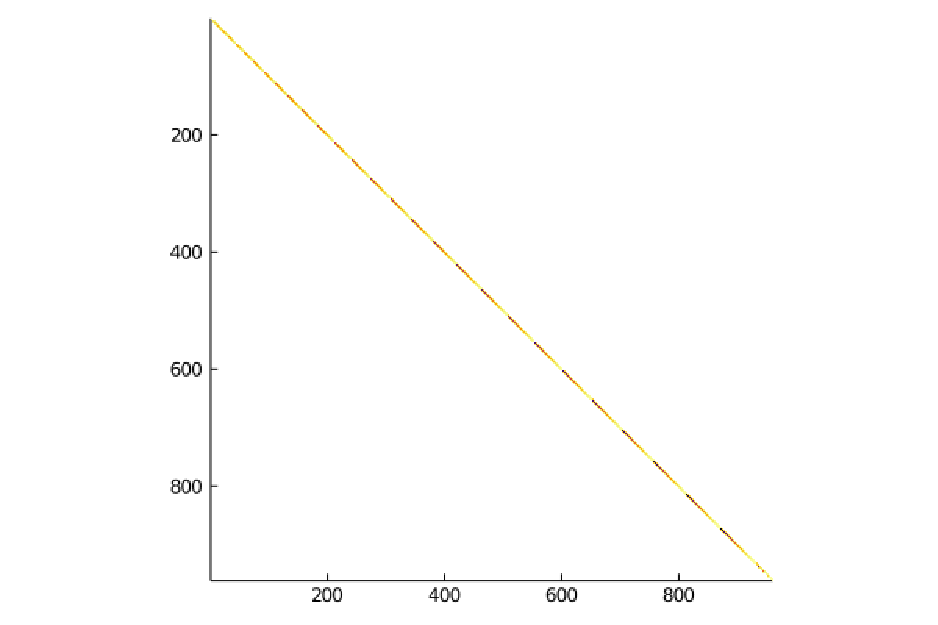
\includegraphics[scale=0.5]{sparsity-of-laplacian}}
		\centering
		\caption{}
	\end{subfigure}\hfil % <-- added
	\begin{subfigure}{0.5\textwidth}
		\centerline{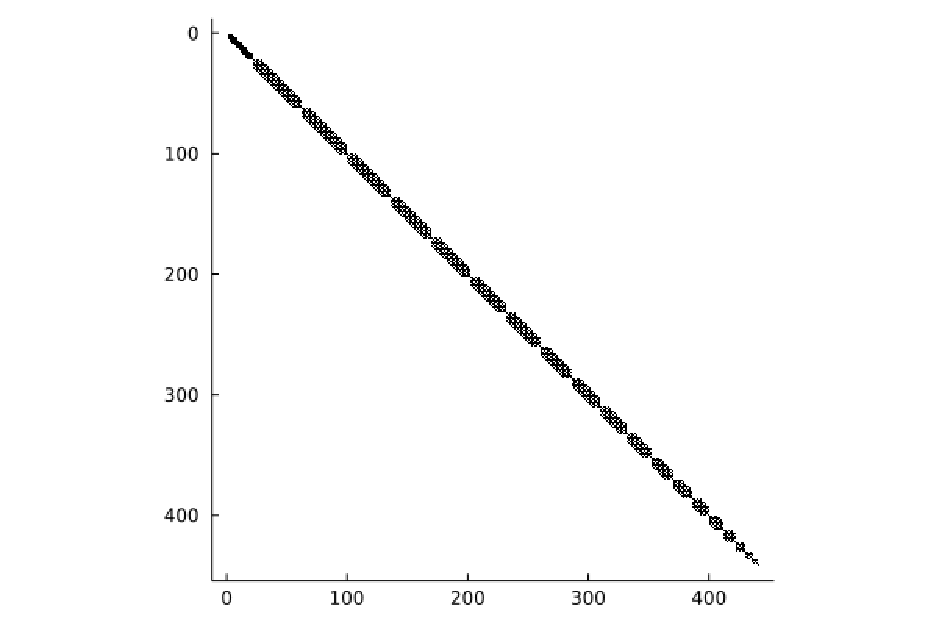
\includegraphics[scale=0.5]{sparsity-of-rho2laplacian}}
		\centering
		\caption{}
	\end{subfigure}\hfil % <-- added

	\medskip
	\begin{subfigure}{0.5\textwidth}
		\centerline{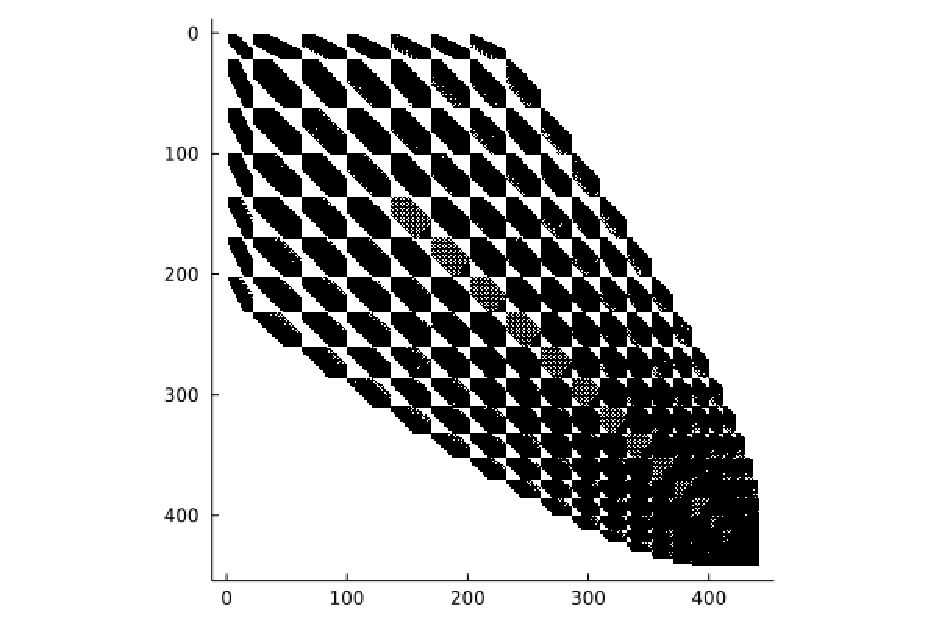
\includegraphics[scale=0.5]{sparsity-of-helmholtz}}
		\centering
		\caption{}
	\end{subfigure}\hfil % <-- added
	\begin{subfigure}{0.5\textwidth}
		\centerline{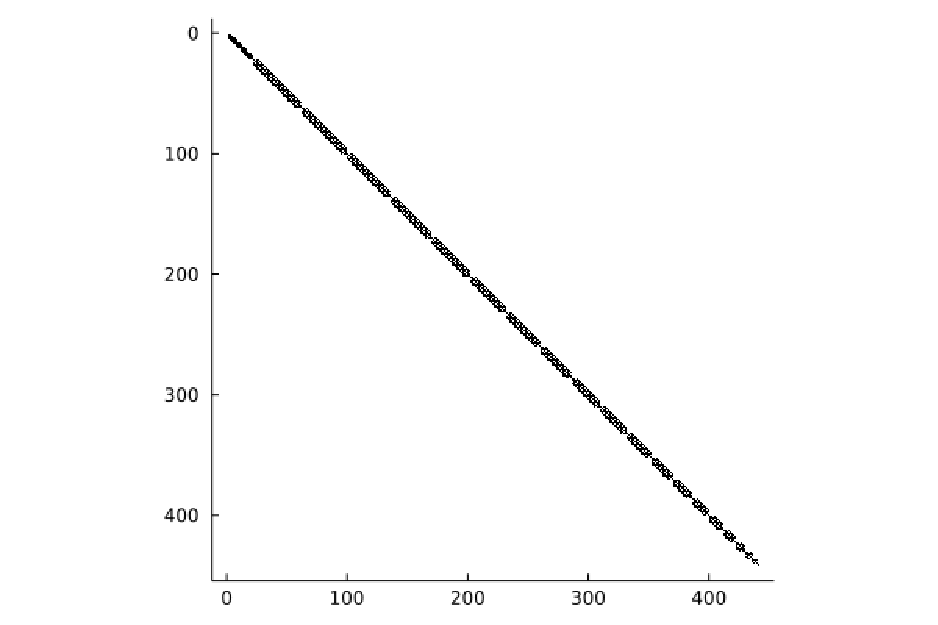
\includegraphics[scale=0.5]{sparsity-of-biharmonic}}
		\centering
		\caption{} 
	\end{subfigure}\hfil % <-- added
	\caption{\enquote{Spy} plots of (differential) operator matrices, showing their sparsity, plotted for $N = 20$. (a) The Laplace-Beltrami operator $\Delta^{(1)}_W$. (b) The $\rho^2$-factored Laplace-Beltrami operator $D_\varphi^{(0)} \: W_\varphi^{(1)} + T^{(0)\to(1)} \: T_W^{(1)\to(0)} \: (D_\theta)^2$. (c) The variable coefficient Helmholtz operator $\Delta^{(1)}_W + k^2 \: T^{(0)\to(1)} \: V({J_x^{(0)}}^\top, {J_y^{(0)}}^\top, {J_z^{(0)}}^\top) \: T_W^{(1)\to(0)}$ for $v(x,y,z) = 1 - (3(x-x_0)^2 + 5(y-y_0)^2 + 2(z-z_0)^2)$ where $(x_0, z_0) := (0.7, 0.2)$, $y_0 := \sqrt{1 - x_0^2 - z_0^2}$ and $k = 200$. (d) The Biharmonic operator $\calB_W^{(2)}$.}
	\label{fig:sc:sparsity}
\end{figure}



\subsection{Further partial differential operators}\label{section:sc:furtherdiffoperators}

General linear partial differential operators with polynomial variable coefficients can be constructed by composing the sparse representations for partial derivatives, conversion between bases, and Jacobi operators. As a canonical example, we can obtain the matrix operator for the $\rho^2$-factored spherical Laplacian $\rho(z)^2 \: \DeltaS$, that will take us from coefficients for expansion in the weighted space $\bigW_N^{(1)}(x,y,z) = \genjacw^{(1,0)}(z) \: \bigscopN^{(1)}(x,y,z)$ to coefficients in the non-weighted space $\bigscopN^{(1)}(x,y,z)$. Note that this construction will ensure the imposition of the Dirichlet zero boundary conditions on $\Omega$, similar to how the Dirichlet zero boundary conditions would be imposed for the operator $\Delta^{(1)}_W$ in \bsrefdef{def:sc:differentialoperators}. The matrix operator for this $\rho^2$-factored spherical Laplacian acting on the coefficients vector is then given by
\bseqn{
	D_\varphi^{(0)} \: W_\varphi^{(1)} + T^{(0)\to(1)} \: T_W^{(1)\to(0)} \: (D_\theta)^2.
}
Importantly, this operator will have banded-block-banded structure, and hence will be sparse, as seen in \bsreffig{fig:sc:sparsity}.

Another desirable operator is the Biharmonic operator $\DeltaS^2$, for which we assume zero Dirichlet and Neumann conditions. That is, 
\bseqn{
	u(x,y,z) &= 0, \quad \pfpx{n}{u}(x,y,z) = \nabla_S u(x,y,z) \cdot \unitvec{n}(x,y,z) = 0 \quad \text{for } (x,y,z) \in \partial\Omega
}
where $\partial\Omega$ is the $z=\alpha$ boundary, and $\unitvec{n}(x,y,z)$ is the outward unit normal vector at the point $(x,y,z)$ on the boundary, i.e. $\unitvec{n}(x,y,z) = \unitvec{n}(\vec x) := {\vec x \over \norm{\vec x}} = \vec x$. The matrix operator for the Biharmonic operator will take us from coefficients in the space $\bigW^{(2)}(x,y,z)$ to coefficients in the space $\bigscopN^{(2)}(x,y,z)$. To construct this, we can simply multiply together two of the spherical Laplacian operators defined in \bsrefdef{def:sc:differentialoperators}, namely $\calL^{(0)\to(2)}$ and $\calL_W^{(2)\to(0)}$:
\bseqn{
	\calB^{(2)}_W := \calL^{(0)\to(2)} \: \calL_W^{(2)\to(0)}.
}
Since the operator $\calL_W^{(2)\to(0)}$ acts on coefficients in the $\bigW^{(2)}(x,y,z)$ space, we ensure that we satisfy the zero Dirichlet and Neumann boundary conditions -- such a function could be written $u(x,y,z) = \genjacw^{(2,0)}(z) \: \tilde u(x,y,z)$ and thus its spherical gradient would be zero on the boundary $z = \alpha$. This allows us to apply the $\calL^{(0)\to(2)}$ operator after, safe in the knowledge that boundary conditions have been accounted for. The sparsity and structure of this biharmonic operator are seen in \bsreffig{fig:sc:sparsity}.


\subsection{Stability of the Laplacian operator}

\begin{figure}[tp]
	\centering
	\begin{subfigure}[b]{0.55\textwidth}
		\centerline{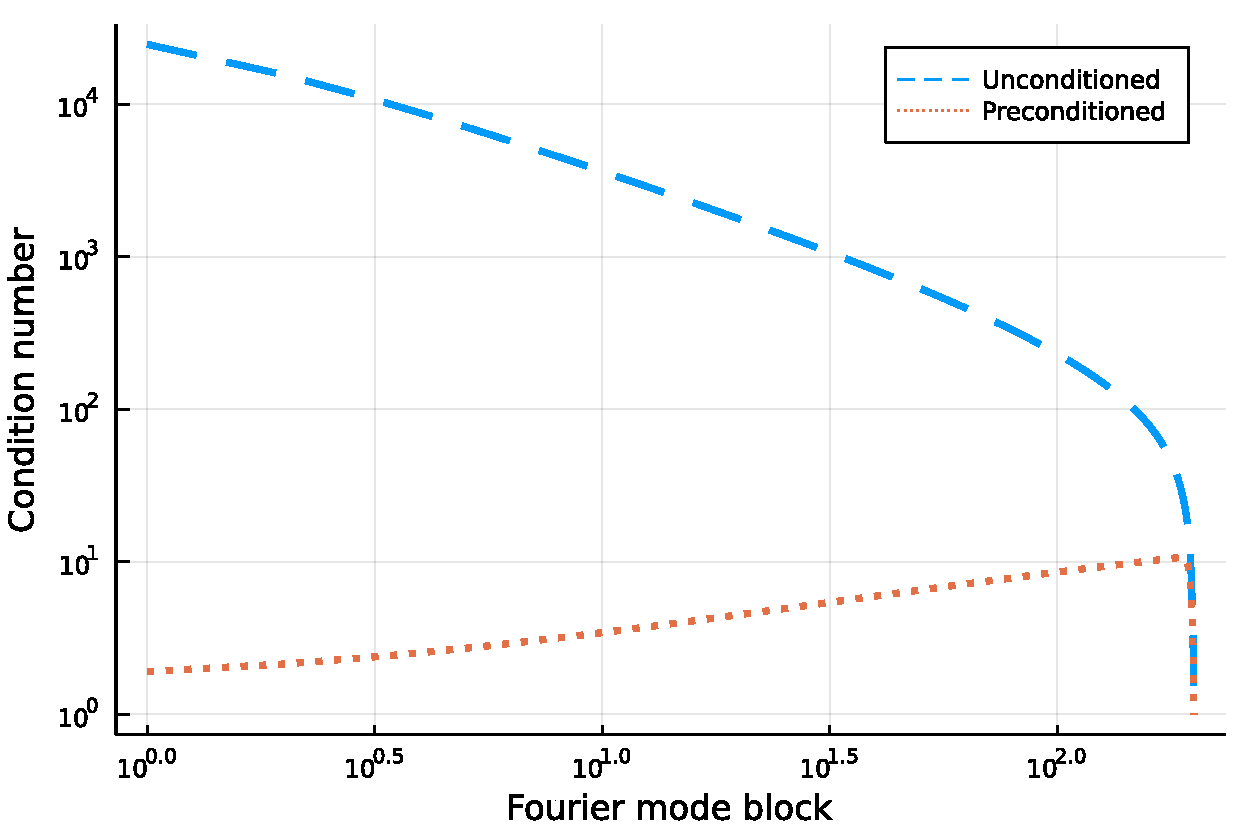
\includegraphics[scale=0.4]{condition-numbers-laplacian-log-N=200}}
	\end{subfigure}
	\hfill%
	
	\begin{subfigure}[b]{0.55\textwidth}
		\centerline{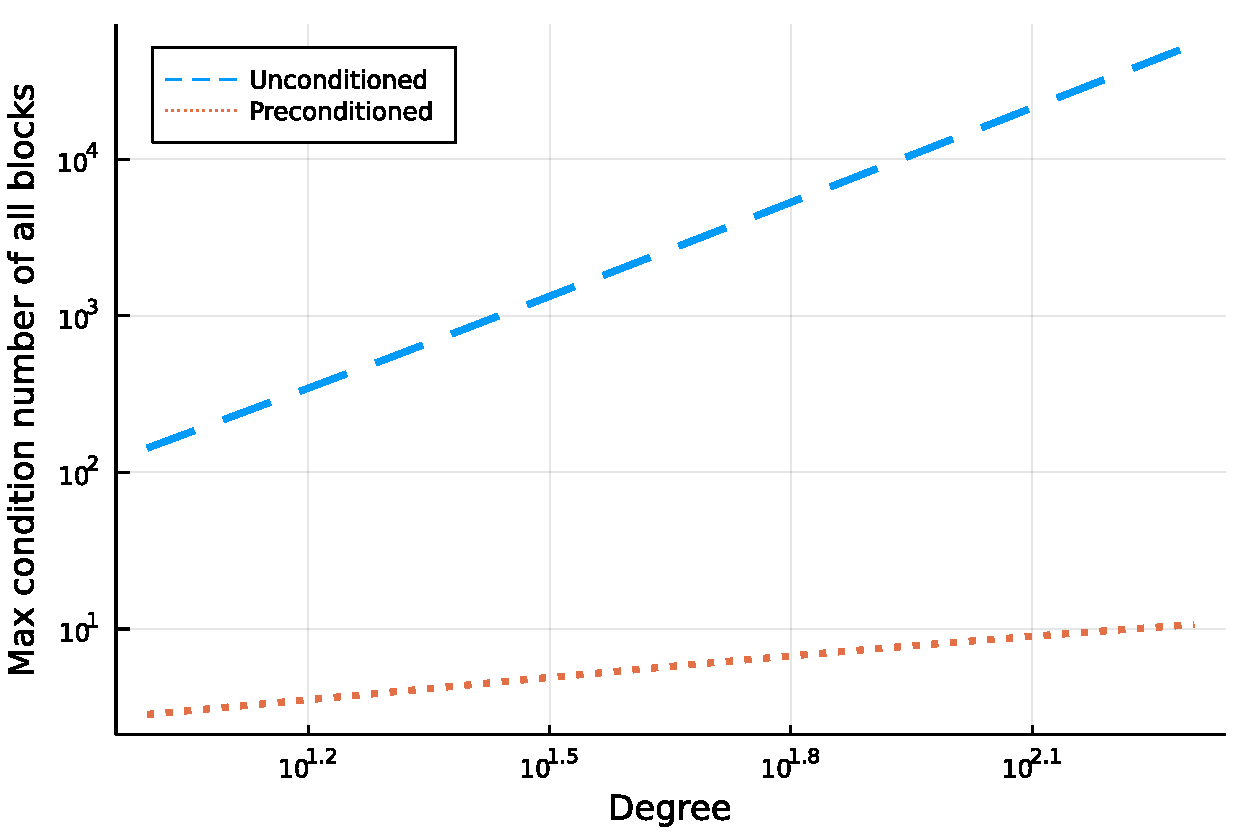
\includegraphics[scale=0.4]{condition-numbers-max-laplacian-log}}
	\end{subfigure}
	\hfill%
	\caption{Plots of the condition number for the Laplacian operator matrix $\Delta^{(1)}_W$ and the preconditioned matrix $P^{-1} \Delta^{(1)}_W$ where $P$ is the matrix of the diagonal of $\Delta^{(1)}_W$. Top: The condition numbers of each diagonal block of $\Delta^{(1)}_W$ for $N = 200$, as well as those for $P^{-1} \Delta^{(1)}_W$. Bottom: The maximum condition number of all diagonal blocks of the Laplacian and the preconditioned Laplacian operators, as the degree $N$ increases.}
	\label{fig:sc:conditionnumbers}
\end{figure}

Denote the condition number of the matrix $A$: 
\bseqn{
	\kappa(A) := \norm{A}_2 \norm{A^{-1}}_2,
}
which encodes how accurate the solution to $A \vc x = \vc b$ is under perturbation.
Since the Laplacian operator is block-diagonal one can determine the condition number from the condition numbers of each block on the diagonal,  and hence deduce the accuracy in solving the Poisson equation, where graphical representations are seen in \bsreffig{fig:sc:conditionnumbers} for the $\Delta^{(1)}_W$ operator matrix. As the degree $N$ increases, the condition numbers of these blocks becomes grows  algebraically fast (at least, the condition number for the first block where $m=0$ does, which will be the largest for each $N$). Fortunately however, by applying a trivial diagonal preconditioning matrix similar to that seen for the ultraspherical method \cite{olver2013fast}, we can significantly bound this growth of the condition numbers -- this is also seen in Figure \bsreffig{fig:sc:conditionnumbers}. The preconditioning matrix chosen is $P^{-1}$, where $P$ is the matrix of the diagonal of $\Delta^{(1)}_W$. 



%
\section{Computational aspects}\label{Section:sc:Computation}

In this section we discuss how to expand and evaluate functions in our proposed basis, and take advantage of the sparsity structure in partial differential operators in practical computational applications.


\subsection{Constructing $\genjac_n^{(a,b)}(x)$}

It is possible to recursively obtain the recurrence coefficients for the $\{\genjac_n^{(a,b)}\}$ OPs in (\ref{eqn:sc:Rrecurrence}), see \cite{snowball2019sparse}, by careful application of the Christoffel--Darboux formula \cite[18.2.12]{DLMF}.


\subsection{Quadrature rule on the spherical cap}\label{section:sc:quadrule}

In this section we construct a quadrature rule that is exact for polynomials on the spherical cap $\Omega$ that can be used to expand functions in the OPs $\scopnkia(x,y,z)$ for a given parameter $a$.

\begin{theorem}\label{theorem:sc:quadrule}
	Let $M_1, M_2 \in \N$ and denote the $M_1$ Gauss quadrature nodes and weights on $[\alpha,1]$ with weight $(t - \alpha)^a$ as $(t_j, w_j^{(t)})$. Further, denote the $M_2$ Gauss quadrature nodes and weights $[-1,1]$ with weight $(1 - x^2)^{-\half}$ as $(s_j, w_j^{(s)})$.
Define for $j = 1,\dots,M_1, \: l=1,\dots,M_2$:
\bseqn{
	x_{l+(j-1)M_2} &:= \rho(t_j) \: s_l, \\
	y_{l+(j-1)M_2} &:= \rho(t_j) \: \sqrt{1-s_l^2}, \\
	z_{l+(j-1)M_2} &:= t_j, \\
	w_{l+(j-1)M_2} &:= w_j^{(t)} w_l^{(s)}.
}
Let $f(x,y,z)$ be a function on $\Omega$, and $N \in \N$. The quadrature rule is then
\bseqn{
	\int_\Omega f(x,y,z) \: \genjacw^{(a,0)}(z) \: \D A \approx \sum_{j=1}^{M} w_j \: \big[ f(x_j, y_j, z_j) + f(-x_j, -y_j, z_j) \big],
}
where $M = M_1 \: M_2$, and the quadrature rule is exact if $f(x,y,z)$ is a polynomial of degree $\le N$ with $M_1 \ge \half (N+1), M_2 \ge N+1$.
\end{theorem}

\begin{remark} 
	Note that the Gauss quadrature nodes and weights $(t_j, w_j^{(t)})$ will have to be calculated, however the Gauss quadrature nodes and weights $(s_j, w_j^{(s)})$ are simply the Chebyshev--Gauss quadrature nodes and weights given explicitly \cite[3.5.23]{DLMF} as $s_j := \cos \fpr(\frac{2j - 1}{2M_2} \pi)$, $w_j^{(s)} := \frac{\pi}{M_2}$.
\end{remark}

\begin{proof}
Let $f : \Omega \to \R$. Define the functions $f_e, f_o : \Omega \to \R$ by 
\bseqn{
	f_e(x,y,z) &:= \half \Big(f(x, y,z) + f(-x, -y,z)\Big), \quad \forall (x,y,z) \in \Omega\\
	f_o(x,y,z) &:= \half \Big(f(x, y,z) - f(-x, -y,z)\Big), \quad \forall (x,y,z) \in \Omega
}
so that $\xvec \mapsto f_e(\xvec, z)$ for fixed $z$ is an even function, and $\xvec \mapsto f_o(\xvec, z)$ for fixed $z$ is an odd function. Note that if $f$ is a polynomial, then $f_e(\rho(t)x, \rho(t)y, t)$ is a polynomial in $t \in [\alpha,1]$ for fixed $(x,y) \in \R^2$. 

Firstly, we note that
\bseqn{
	\int_0^{2\pi} g\big(\cos \theta, \sin\theta\big) \: \D \theta &= \int_{-1}^1 \Big[ g\big(x, \sqrt{1-x^2}\big) + g\big(x, -\sqrt{1-x^2}\big) \Big] \frac{\D x}{\sqrt{1-x^2}} \\
	&= \int_{-1}^1 \Big[ g\big(x, \sqrt{1-x^2}\big) + g\big(-x, -\sqrt{1-x^2}\big) \Big] \frac{\D x}{\sqrt{1-x^2}}
}
for any function $g$, using a change of variables $x \to -x$ for the second term in the integral. Then, integrating the even function $f_e$ we have
\bseqn{
	&\int_\Omega f_e(x,y,z) \: \genjacw^{(a,0)}(z) \: \D A \\
	&\quad \quad = \int_\alpha^1 \genjacw^{(a,0)}(z) \: \Big( \int_0^{2\pi} f_e\big(\rho(z)\cos\theta,\rho(z)\sin\theta, z\big) \: \D \theta \Big) \: \D z \\
	&\quad \quad = \int_\alpha^1 \genjacw^{(a,0)}(z) \: \Big( \int_{-1}^1 \Big[ f_e\big(\rho(z)x,\rho(z)\sqrt{1-x^2}, z\big) \\
	&\quad \quad \quad \quad \quad \quad \quad \quad \quad \quad \quad \quad + f_e\big(-\rho(z)x, - \rho(z)\sqrt{1-x^2}, z\big) \Big] \: \frac{\D x}{\sqrt{1-x^2}} \Big) \: \D z \\
	&\quad \quad = 2 \int_\alpha^1 \genjacw^{(a,0)}(z) \: \Big( \int_{-1}^1 f_e\big(\rho(z)x,\rho(z)\sqrt{1-x^2}, z\big) \: \frac{\D x}{\sqrt{1-x^2}} \Big) \: \D z \\
	&\quad \quad \approx 2 \int_\alpha^1 \genjacw^{(a,0)}(z) \: \Big( \sum_{l=1}^{M_2} w_l^{(s)} f_e\big(\rho(z) s_l, \rho(z) \sqrt{1 - s_l^2}, z\big) \Big) \: \D z \quad (\star) \\
	&\quad \quad \approx 2 \sum_{j=1}^{M_1} w_j^{(t)} \sum_{l=1}^{M_2} w_l^{(s)} f_e\big(\rho(t_j) s_l, \rho(t_j) \sqrt{1 - s_l^2}, t_j\big) \quad (\star \star) \\
	&\quad \quad = 2 \sum_{k=1}^{M_1 M_2}  w_j \: f_e(x_j, y_j, z_j).
}
Suppose $f$ is a polynomial in $x,y,z$ of degree $N$, and hence that $f_e$ is a degree $\le N$ polynomial. It follows that $s \mapsto f_e\big(\rho(z)s,\rho(z)\sqrt{1-s^2}, z\big)$ for fixed $z$ is then a polynomial of degree $\le N$. We therefore achieve equality at $(\star)$ if $2M_2 - 1 \ge N$ and we achieve equality at $(\star \star)$ if also $2M_1 - 1 \ge N$.

Integrating the odd function $f_o$ results in
\bseqn{
	&\int_\Omega f_o(x,y,z) \: \genjacw^{(a,0)}(z) \: \D A \\
	&\quad \quad = \int_\alpha^1 \genjacw^{(a,0)}(z) \: \Big( \int_0^{2\pi} f_o\big(\rho(z)\cos\theta,\rho(z)\sin\theta, z)\big) \: \D \theta \Big) \: \D z \\
	&\quad \quad = \int_\alpha^1 \genjacw^{(a,0)}(z) \: \Big( \int_{-1}^1 \Big[ f_o\big(\rho(z)x,\rho(z)\sqrt{1-x^2}, z\big) \\
	&\quad \quad \quad \quad \quad \quad \quad \quad \quad \quad \quad \quad + f_o\big(-\rho(z)x, - \rho(z)\sqrt{1-x^2}, z\big) \Big] \: \frac{\D x}{\sqrt{1-x^2}} \Big) \: \D z \\
	&\quad \quad = 0.
}
since $f_o(x,y,z) = - f_o(-x, -y, z)$. Hence, for a polynomial $f$ in $x,y,z$ of degree $N$,
\bseqn{
	\int_\Omega f(x,y,z) \: \genjacw^{(a,0)}(z) \: \D A &= \int_\Omega \Big(f_e(x,y,z) + f_o(x,y,z)\Big) \:  \genjacw^{(a,0)}(z) \: \D A  \\
	&= \int_\Omega f_e(x,y,z) \: \genjacw^{(a,0)}(z) \: \D A \\
	&= \sum_{j=1}^{M}  w_j \: f_e(x_j, y_j, z_j),
}
where $M = M_1 M_2$ and $2M_1 - 1 \ge N, 2M_2 - 1 \ge N$.
\end{proof}


\subsection{Obtaining the coefficients for expansion of a function on the spherical cap}\label{section:sc:expandingfunctions}

Fix $a \in \R$. Then for any function $f : \Omega \to \R$ we can express $f$ by
\bseqn{
	f(x,y,z) \approx \sum_{k=0}^N \bigscopNka(x,y,z)^\top \: \vec{f}_k = \bigscopNa(x,y,z)^\top \: \vec{f}
}
for N sufficiently large, where $\bigscopNka, \bigscopNa$ is defined in \bsrefeqns{eqn:sc:OPdefNka}{eqn:sc:OPdefNa} and where
\bseqn{
	\vec{f}_k &:= 
		\begin{pmatrix}
			f_{k,k,0} \\
			f_{k,k,1} \\
			\vdots \\
			f_{N,k,0} \\
			f_{N,k,1}
		\end{pmatrix} \in \R^{2(N-k+1)} \quad \text{for } n = 1,2,\dots,N, \quad
	\vec{f}_0 := 
		\begin{pmatrix}
			f_{0,0,0} \\
			\vdots \\
			f_{N,0,0}
		\end{pmatrix} \in \R^{N+1}, \\
	\vec{f} &:= 
		\begin{pmatrix}
			\vec{f}_0 \\
			\vdots \\
			\vec{f}_N
		\end{pmatrix} \in \R^{2(N+1)^2}, \quad \quad
	f_{n,k,i} := \ip< f, \: \scopnkia>_{\scopa} \: \norm{\scopnkia}^{-2}_{\scopa}.
}
Recall from \bsrefeqn{eqn:sc:normscop} that $\norm{\scopnkia}^2_{\scopa} = \normgenjac^{(a,2k)} \: \pi$. Using the quadrature rule detailed in \bsrefsection{section:sc:quadrule} for the inner product, we can calculate the coefficients $f_{n,k,i}$ for each $n = 0,\dots,N$, $k = 0,\dots,n$, $i = 0,1$: 
\bseqn{
	f_{n,k,i} &= \frac{1}{\normgenjac^{(a,2k)} \: \pi} \sum_{j=1}^{M} w_j \big[ f(x_j, y_j, z_j) \scopnkia(x_j, y_j, z_j) \\
	&\quadeight \quad + f(-x_j, -y_j, z_j) \scopnkia(-x_j, -y_j, z_j) \big] \\
	&= \frac{1}{M_2 \: \normgenjac^{(a,2k)}} \sum_{j=1}^{M_1} w^{(t)}_j \sum_{l=1}^{M_2} \big[ f(x_j, y_j, z_j) \scopnkia(x_j, y_j, z_j) \\
	&\quadeight \quadfour + f(-x_j, -y_j, z_j) \scopnkia(-x_j, -y_j, z_j) \big]
}
where the quadrature nodes and weights are those from \bsreftheorem{theorem:sc:quadrule}, and $M = M_1 M_2$ with $2M_1 - 1 \ge N, M_2 - 1 \ge N$ (i.e. we can choose $M_2 := N + 1$ and $M_1 := \ceil{\frac{N+1}{2}}$).

\remark{While it may be possible to leverage fast transforms, as in \cite{slevinsky2018use,slevinsky2019fast}, to speed up the calculation of the coefficients, this remains an open question.}



\subsection{Function evaluation}\label{section:sc:functionevaluation}

For a function $f$, with coefficients vector $\vec{f}$ for expansion in the $\{\scopnki\}$ basis as determined via the method in \bsrefsection{section:sc:expandingfunctions} up to order $N$, we can use the Clenshaw algorithm to evaluate the function at a point $(x,y,z) \in \Omega$ as follows, as we have seen for the spherical harmonics and disk-slice in \bsrefchapter{CHAPTER:sphericalharmonics} and \bsrefchapter{CHAPTER:diskslice} respectively. Let $A_n, B_n, \Dnt, C_n$ be the Clenshaw matrices from \bsrefdef{def:sc:clenshawmats}, and define the rearranged coefficients vector $\tilde{\vec{f}}$ via
\bseqn{
	{\vec{f}}_n &:= 
		\begin{pmatrix}
			f_{n,0,0} \\
			f_{n,1,0} \\
			f_{n,1,1} \\
			\vdots \\
			f_{n,n,0} \\
			f_{n,n,1}
		\end{pmatrix} \in \R^{2(N+1)} \quad \text{for } n = 1,2,\dots,N, \quad
	{\vec{f}}_0 = f_{0,0,0} \in \R, \\
	{\vec{f}} &:= 
		\begin{pmatrix}
			{\vec{f}}_0 \\
			\vdots \\
			{\vec{f}}_N
		\end{pmatrix} \in \R^{(N+1)^2}.
}
The trivariate Clenshaw algorithm works similar to the bivariate Clenshaw algorithm introduced in \cite{olver2019triangle} for expansions in the triangle:
\bseqn{
	\quad &\text{1) } \text{Set } \vec{\xi}_{N+2} = \bold{0}, \: \vec{\xi}_{N+2} = \bold{0}. \\
	\quad &\text{2) } \text{For } n = N:-1:0 \\
	\quad & \quad \quad \quad \text{set } \vec{\xi}_{n}^T = {{\vec{f}}_n}^T - \vec{\xi}_{n+1}^T D^T_n (B_n - G_n(x,y,z)) -  \vec{\xi}_{n+2}^T D^T_{n+1}C_{n+1} \\
	\quad &\text{3) } \text{Output: } f(x,y,z) \approx \vec{\xi}_{0} \: \bigscopta_{0}  = \xi_{0} \: \scopa_0
}


\subsection{Calculating non-zero entries of the operator matrices}\label{section:sc:Computation-operatormatrices}

The proofs of \bsreftheorem{theorem:sc:sparsityofdifferentialoperators} and \bsreflemma{lemma:sc:sparsityofparametertransformationoperators} provide a way to calculate the non-zero entries of the operator matrices given in \bsrefdef{def:sc:differentialoperators} and \bsrefdef{def:sc:parametertransformationoperators}. We can simply use quadrature to calculate the 1D inner products, which has a complexity of $\bigO(N^2)$. This proves much cheaper computationally than using the 3D quadrature rule to calculate the surface inner products, which has a complexity of $\bigO(N^3)$.


\subsection{Obtaining operator matrices for variable coefficients}\label{section:sc:operatorclenshaw}

The Clenshaw algorithm outlined in \bsrefsection{section:sc:functionevaluation} can also be used with Jacobi matrices $J^{(a)}_x, J^{(a)}_y, J^{(a)}_z$ replacing the point $(x,y,z)$. Let $v : \Omega \to \R$ be the function that we wish to obtain an operator matrix $V$ for $v$, so that
\bseqn{
	v(x,y,z) \: f(x,y,z) = v(x,y,z) \: \vec{f} \: \bigscopta(x,y,z) = (V \vec{f})^\top \: \bigscopta(x,y,z),
}
i.e. $V \vec{f}$ is the coefficients vector for the function $v(x,y,z) \: f(x,y,z)$. 

To this end, let $\tilde{\vec{v}}$ be the coefficients for expansion up to order $N$ in the $\{\scopnki\}$ basis of $v$ (rearranged as in \bsrefsection{section:sc:functionevaluation} so that $v(x,y,z) = {\vec{v}}^\top \: \bigscopta(x,y,z)$). Denote $X := (J_x^{(a)})^\top$, $Y := (J_y^{(a)})^\top$, $Z := (J_z^{(a)})^\top$. The operator $V$ is then the result of the following:
\bseqn{
	\quad &\text{1) } \text{Set } \vec{\xi}_{N+2} = \bold{0}, \: \vec{\xi}_{N+2} = \bold{0}. \\
	\quad &\text{2) } \text{For } n = N:-1:0 \\
	\quad & \quad \quad \quad \text{set } \vec{\xi}_{n}^T = {\tilde{\vec{v}}_n}^T - \vec{\xi}_{n+1}^T D^T_n \big(B_n - G_n(X, Y, Z)\big) -  \vec{\xi}_{n+2}^T D^T_{n+1}C_{n+1} \\
	\quad &\text{3) } \text{Output: } V = v(X, Y, Z) \approx \vec{\xi}_{0} \: \bigscopta_{0}  = \xi_{0} \: \scopa_0
}
where at each iteration, $\vec{\xi}_n$ is a vector of matrices.



%
\section{Examples on spherical caps with zero Dirichlet conditions}\label{Section:sc:Examples}

We now demonstrate how the sparse linear systems constructed as above can be used to efficiently solve PDEs with zero Dirichlet conditions on the spherical cap defined by $\Omega$. We consider Poisson, inhomogeneous variable coefficient Helmholtz equation and the Biharmonic equation, as well as a time dependent heat equation, demonstrating the versatility of the approach.

\subsection{Poisson}

% FIGURES

\begin{figure}[tp]
	\centering
	\begin{subfigure}{0.85\textwidth}
		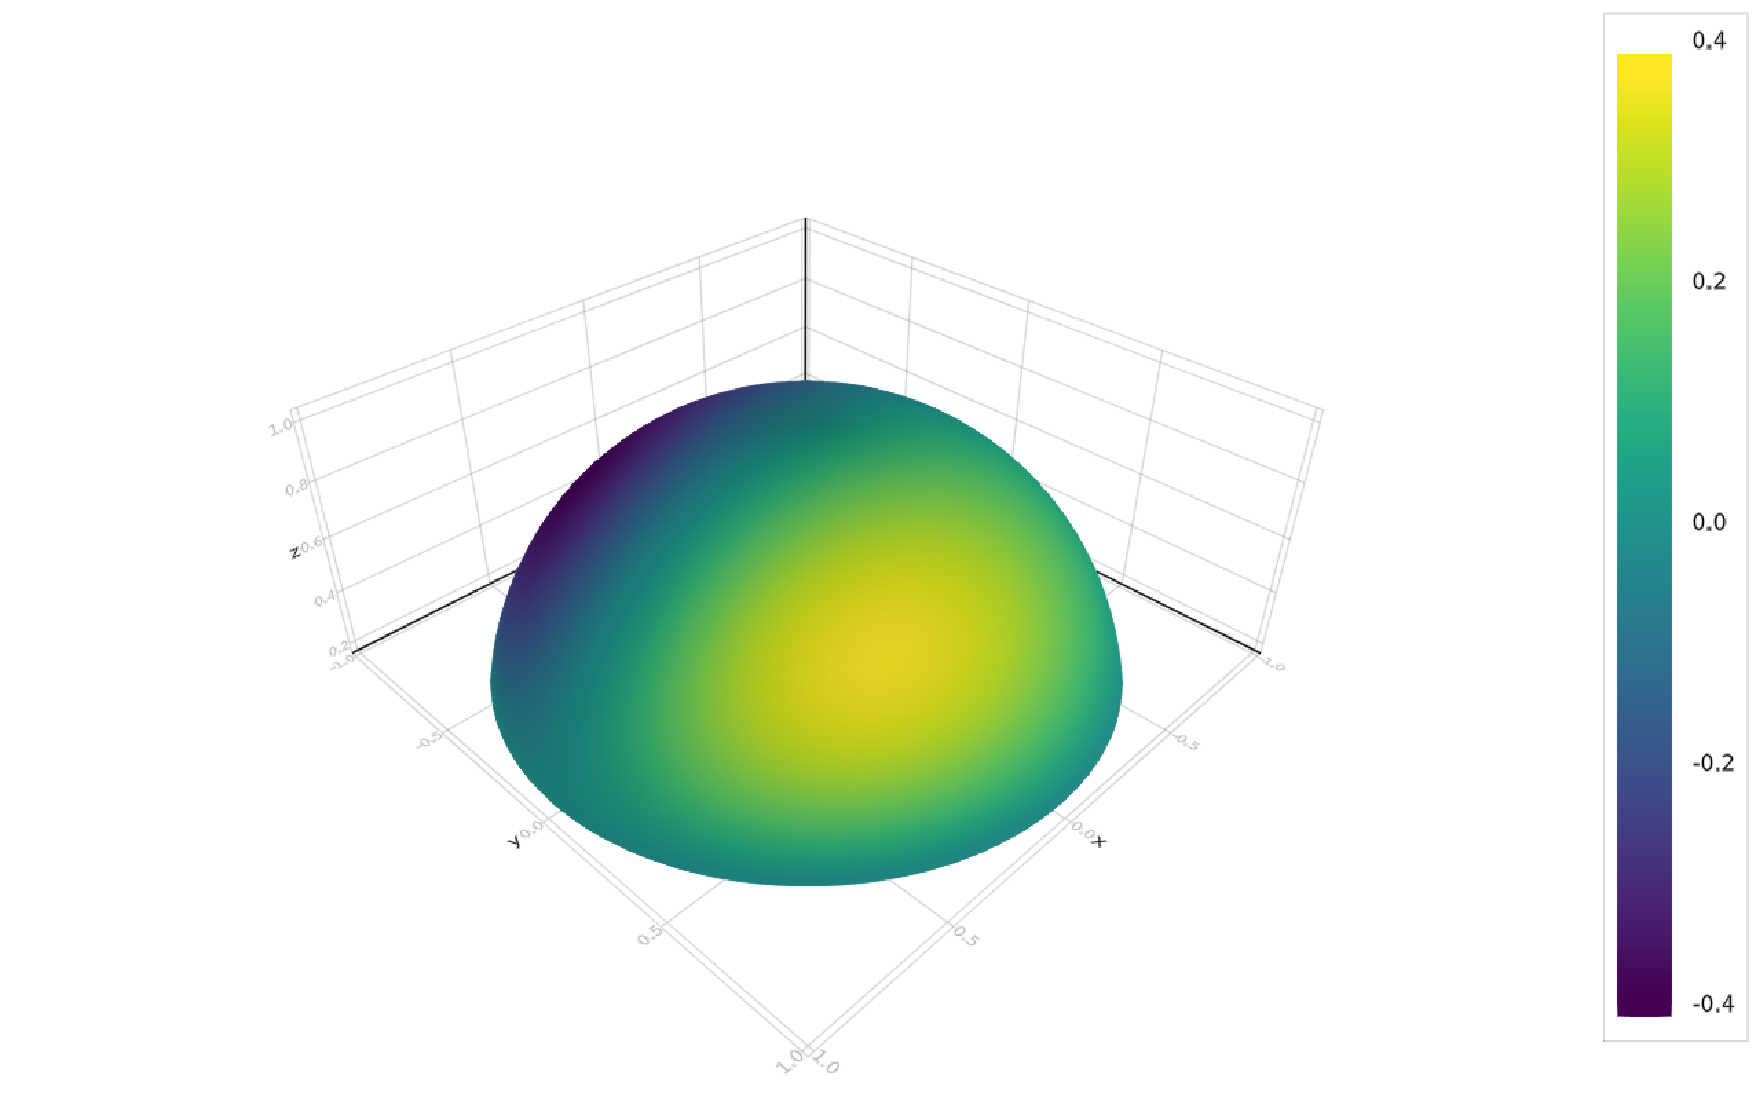
\includegraphics[scale=0.4]{poisson-u=wyexpx-N=60}
	\end{subfigure}
	\hfill%
	
	\begin{subfigure}{0.55\textwidth}
		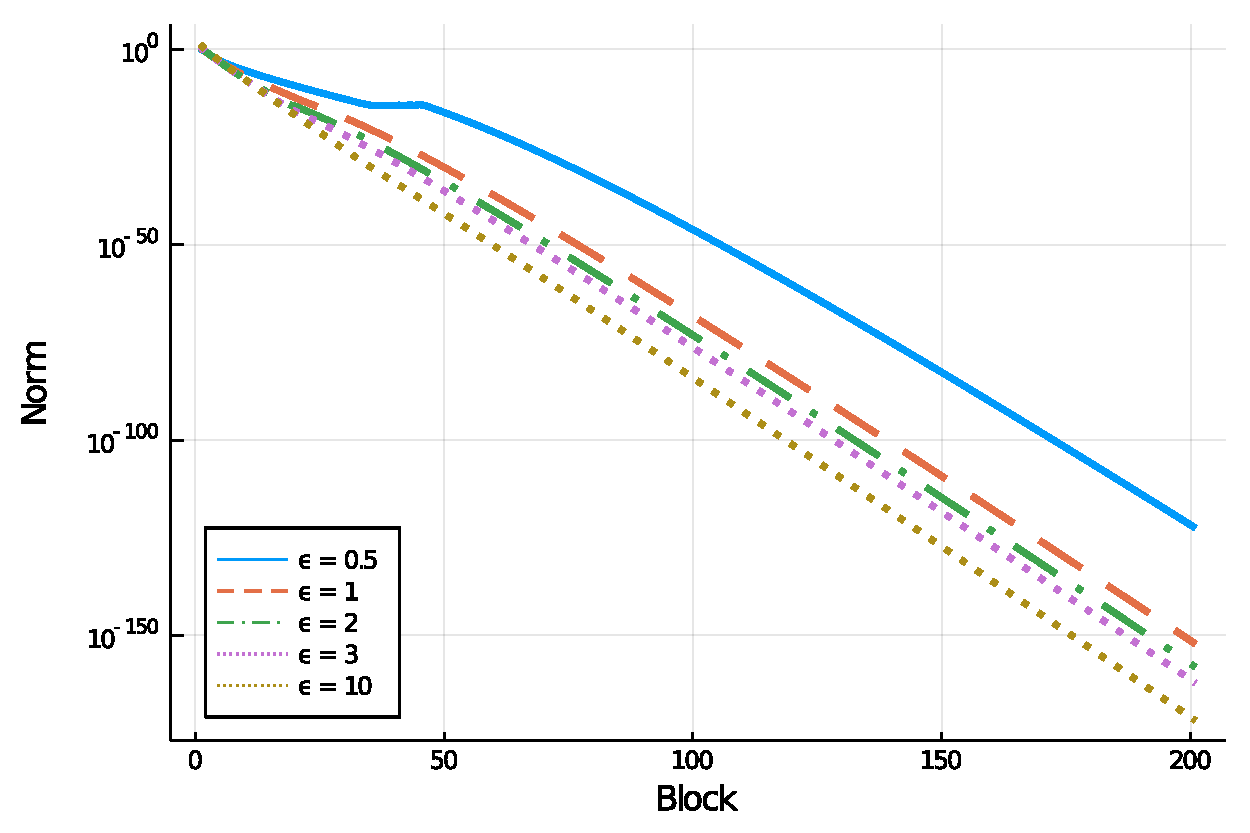
\includegraphics[scale=0.4]{solutionblocknorms-poisson-epsilonfun-N=200}
	\end{subfigure}
	\hfill%
	\caption{Top: The computed solution to $\Delta u = f$ with zero boundary conditions with $f(x,y,z) = - 2 e^x y z (2+x) + \genjacw^{(1,0)}(z) e^x (y^3 + z^2 y - 4xy - 2y)$. Bottom: The norms of each block of the computed solution of the Poisson equation with right hand side function $f(x,y,z) = \norm{\xvec - (\epsilon + 1 / \sqrt{3}) \; (1,1,1)^\top }$ for different $\epsilon$ values. This indicates spectral convergence.}
	\label{fig:sc:poisson}
\end{figure}

% END FIGURES

The Poisson equation is the classic problem of finding $u(x,y,z)$ given a function $f(x,y,z)$ such that:
\bseqnnumber{
	\begin{cases}
\DeltaS u(x,y,z) = f(x,y,z) &\quad \text{in } \Omega \\
		u(x,y,z) = 0& \quad \text{on } \partial \Omega
	\end{cases}
	\label{eqn:sc:poisson}
}
noting the imposition of zero Dirichlet boundary conditions on $u$.

We can tackle the problem as follows. Choose an $N \in \N$ large enough for the problem, and denote the coefficient vector for expansion of $u$ in the $\bigWNi$ OP basis up to degree $N$ by $\mathbf{u}$, and the coefficient vector for expansion of $f$ in the $\bigscopNi$ OP basis up to degree $N$ by $\mathbf{f}$. Since $f$ is known, we can obtain $\mathbf{f}$ using the quadrature rule in \bsrefsection{section:sc:expandingfunctions}. In matrix-vector notation, our system hence becomes:
\bseqn{
    \Delta_W^{(1)} \mathbf{u} = \mathbf{f}
}
which can be solved to find $\mathbf{u}$.
In \bsreffig{fig:sc:poisson} we see the solution to the Poisson equation with zero boundary conditions given in \bsrefeqn{eqn:sc:poisson} in the disk-slice $\Omega$. In \bsreffig{fig:sc:poisson} we also show the norms of each block of calculated coefficients of the approximation for four right-hand sides of the Poisson equation with $N = 200$, that is, $(N+1)^2 = 40,401$ unknowns. The right hand sides we choose here are given by
\bseqn{
	f(x,y,z) &= \norm{\Big(x - (\epsilon + 1 / \sqrt{3}), \: y - (\epsilon + 1 / \sqrt{3}), \: z - (\epsilon + 1 / \sqrt{3})\Big)^\top}
}
for differing choices of $\epsilon$ -- this parameter serves to alter the distance from which we would have a singularity. In the plot, a \enquote{block} is simply the group of coefficients corresponding to OPs of the same degree, and so the plot shows how the norms of these blocks decay as the degree of the expansion increases. Thus, the rate of decay in the coefficients is a proxy for the rate of convergence of the computed solution: as typical of spectral methods, we expect the numerical scheme to converge at the same rate as the coefficients decay. We see that we achieve spectral convergence for these examples.


\subsection{Inhomogeneous variable-coefficient Helmholtz}

\begin{figure}[tp]
	\centering
	\begin{subfigure}{0.85\textwidth}
		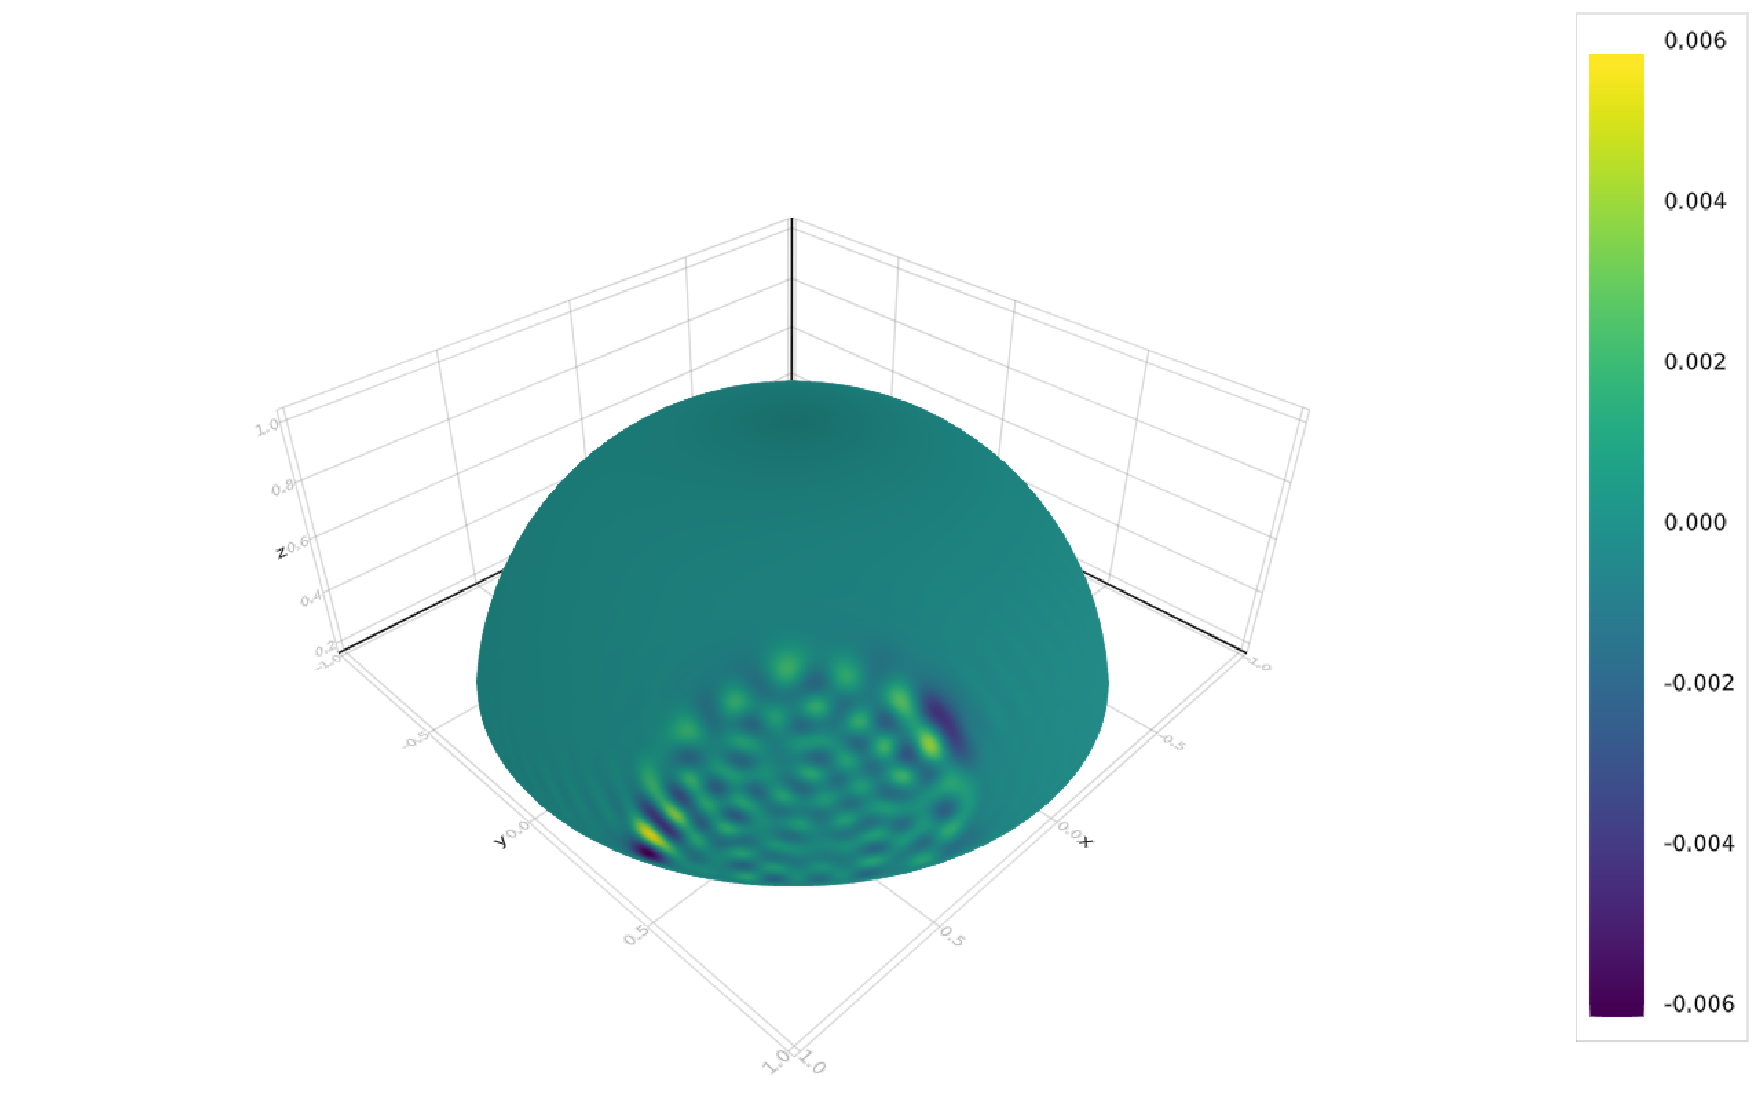
\includegraphics[scale=0.4]{helmholtz-f=wyexpx-N=60-n=300}
	\end{subfigure}
	
	\begin{subfigure}{0.55\textwidth}
		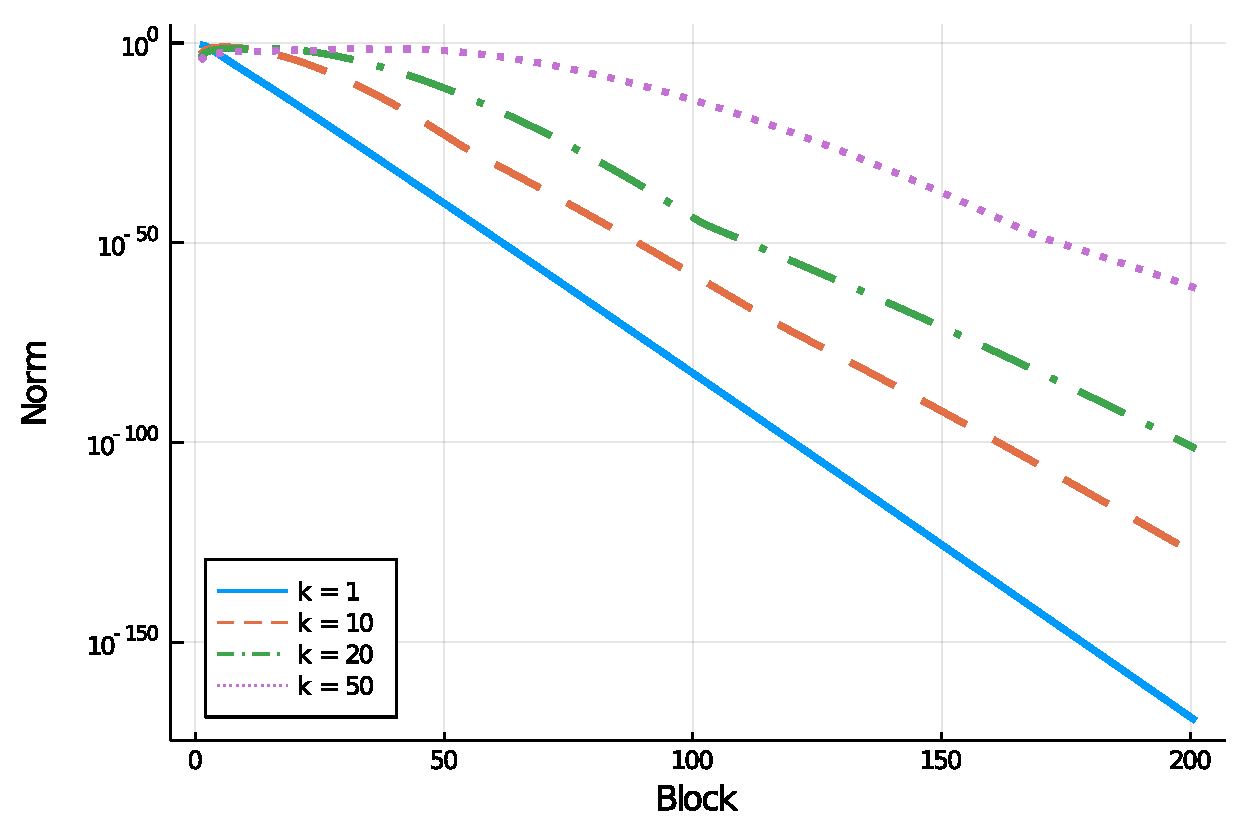
\includegraphics[scale=0.4]{solutionblocknorms-helmholtz-varyingk-N=200}
	\end{subfigure}
	\caption{Top: The computed solution to $\Delta u + k^2 \: v \: u = f$ with zero boundary conditions with $f(x,y,z) = y e^x (z - \alpha) $, $v(x,y,z) = 1 - (3(x-x_0)^2 + 5(y-y_0)^2 + 2(z-z_0)^2)$ where $(x_0, z_0) := (0.7, 0.2)$, $y_0 := \sqrt{1 - x_0^2 - z_0^2}$ and $k = 100$. Bottom: The norms of each block of the computed solution of the Helmholtz equation with the right hand side function $f(x,y,z) = 1$ and the same function $v(x,y,z)$, for various $k$ values. This indicates spectral convergence.}
	\label{fig:sc:helmholtz}
\end{figure}

\begin{figure}[tp]
	\centering % <-- added
	\centerline{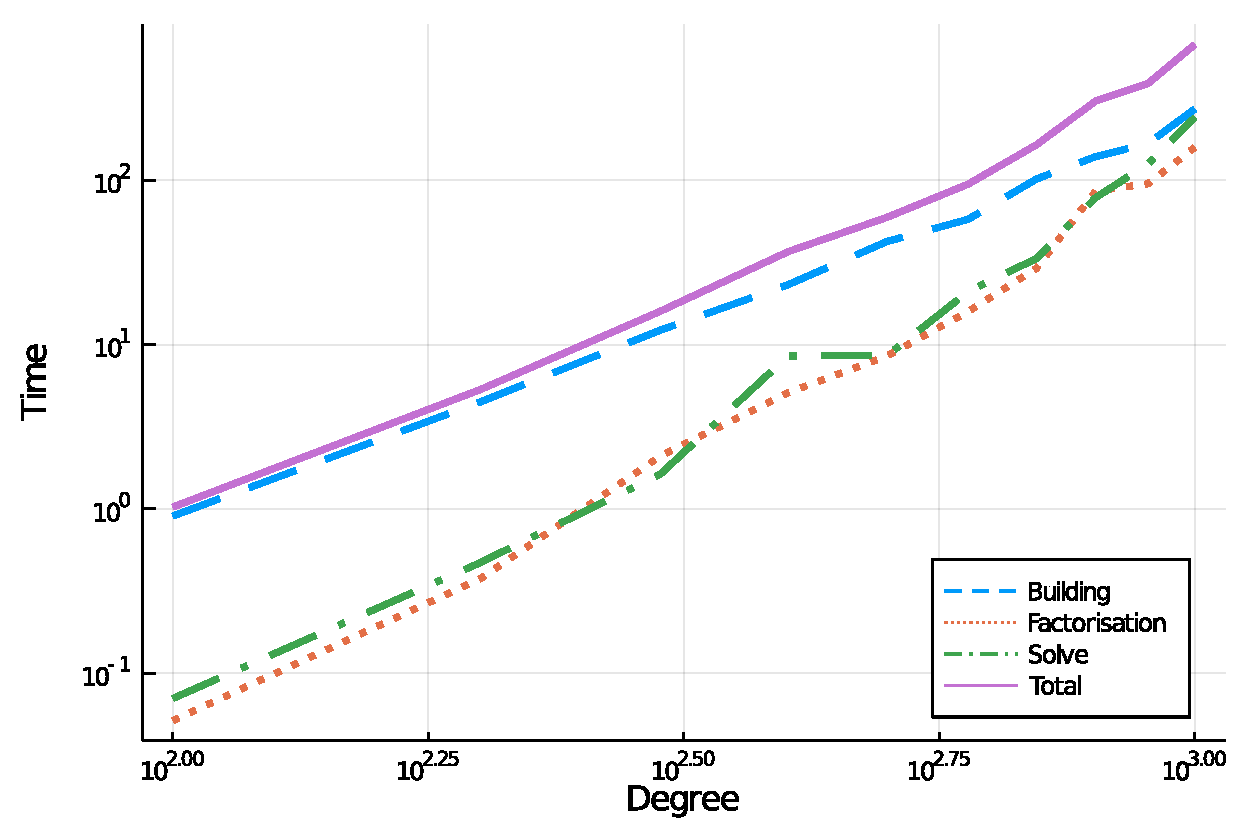
\includegraphics[scale=0.4]{complexity-Nend=1000}}
	\caption{Time in seconds to build and solve the system $\big[\DeltaS + v(x,y,z) \big] \: u(x,y,z) = f(x,y,z)$, for a rotationally invariant $v(x,y,z) = v(z)$. This demonstrates that the approach is roughly of order $\bigO(N^2)$, where $N$ is the degree to which we approximate the solution (the number of unknowns is then $(N+1)^2$). Here, we used $f = -2e^{x}yz(2+x) + (z - \alpha) e^{x} (y^3 + z^2 y - 4xy - 2y)$ and $v(x,y,z) = v(z) = \cos(z)$.}
	\label{fig:sc:complexity}
\end{figure}

Find $u(x,y)$ given functions $v$, $f : \Omega \to \R$ such that:
\bseqnnumber{
	\begin{cases}
    		\DeltaS u(x,y,z) + k^2 \: v(x,y,z) \; u(x,y,z) = f(x,y,z) &\quad \text{in } \Omega \\
		u(x,y,z) = 0 &\quad \text{on } \partial \Omega
	\end{cases}
	\label{eqn:sc:helmholtz}
}
where $k \in \R$, noting the imposition of zero Dirichlet boundary conditions on $u$.

We can tackle the problem as follows. Denote the coefficient vector for expansion of $u$ in the $\bigWNi$ OP basis up to degree $N$ by $\mathbf{u}$, and the coefficient vector for expansion of $f$ in the $\bigscopNi$ OP basis up to degree $N$ by $\mathbf{f}$. Since $f$ is known, we can obtain  the coefficients $\mathbf{f}$ using the quadrature rule in \bsrefsection{section:sc:expandingfunctions}. 

Define $X := (J_x^{(0)})^\top$, $Y := (J_y^{(0)})^\top$, $Z := (J_z^{(0)})^\top$. We can obtain the matrix operator for the variable-coefficient function $v(x,y,z)$ by using the Clenshaw algorithm with matrix inputs as the Jacobi matrices $X, Y, Z$, yielding an operator matrix of the same dimension as the input Jacobi matrices a la the procedure introduced in \cite{olver2019triangle}. We can denote the resulting operator acting on coefficients in the $\bigscopNo$ space by $v(X, Y, Z)$. In matrix-vector notation, our system hence becomes:
\bseqn{
    (\Delta_W^{(1)} + k^2 \:T^{(0)\to(1)} \: V \: T_W^{(1)\to(0)}) \: \mathbf{u} = \mathbf{f}
}
which can be solved to find $\mathbf{u}$. We can see the sparsity and structure of this matrix system in \bsreffig{fig:sc:sparsity} with $v(x,y,z) = zxy^2$ as an example. In \bsreffig{fig:sc:helmholtz} we see the solution to the inhomogeneous variable-coefficient Helmholtz equation with zero boundary conditions given in \bsrefeqn{eqn:sc:helmholtz} in the spherical cap $\Omega$, with $f(x,y,z) = y e^x \genjacw^{(1,0)}(z)$, $v(x,y,z) = 1 - (3(x-x_0)^2 + 5(y-y_0)^2 + 2(z-z_0)^2)$ where $(x_0, z_0) := (0.7, 0.2)$, $y_0 := \sqrt{1 - x_0^2 - z_0^2}$ and $k = 100$. In \bsreffig{fig:sc:helmholtz} we also show the norms of each block of calculated coefficients for the approximation of the solution to the inhomogeneous variable-coefficient Helmholtz equation with various $k$ values. Here, we use $N = 200$, that is, $(N+1)^2 = 40,401$ unknowns. Once again, the rate of decay in the coefficients is a proxy for the rate of convergence of the computed solution, and we see that we achieve spectral convergence.

In \bsreffig{fig:sc:complexity} we plot the time taken\footnote{measured using the \enquote{@belapsed} macro from the BenchmarkTools.jl package \cite{BenchmarkTools.jl-2016} in Julia.} to construct the operator for $\DeltaS + v(x,y,z)$, with a rotationally invariant $v(x,y,z) = v(z) = \cos z$, and solve a zero boundary condition Helmholtz problem. The plot demonstrates that as we increase the degree of approximation $N$, we achieve a complexity of an optimal $\bigO(N^2)$.

What about other boundary conditions? 

\subsection{Biharmonic equation}

\begin{figure}[tp]
	\centering
	\begin{subfigure}{0.85\textwidth}
		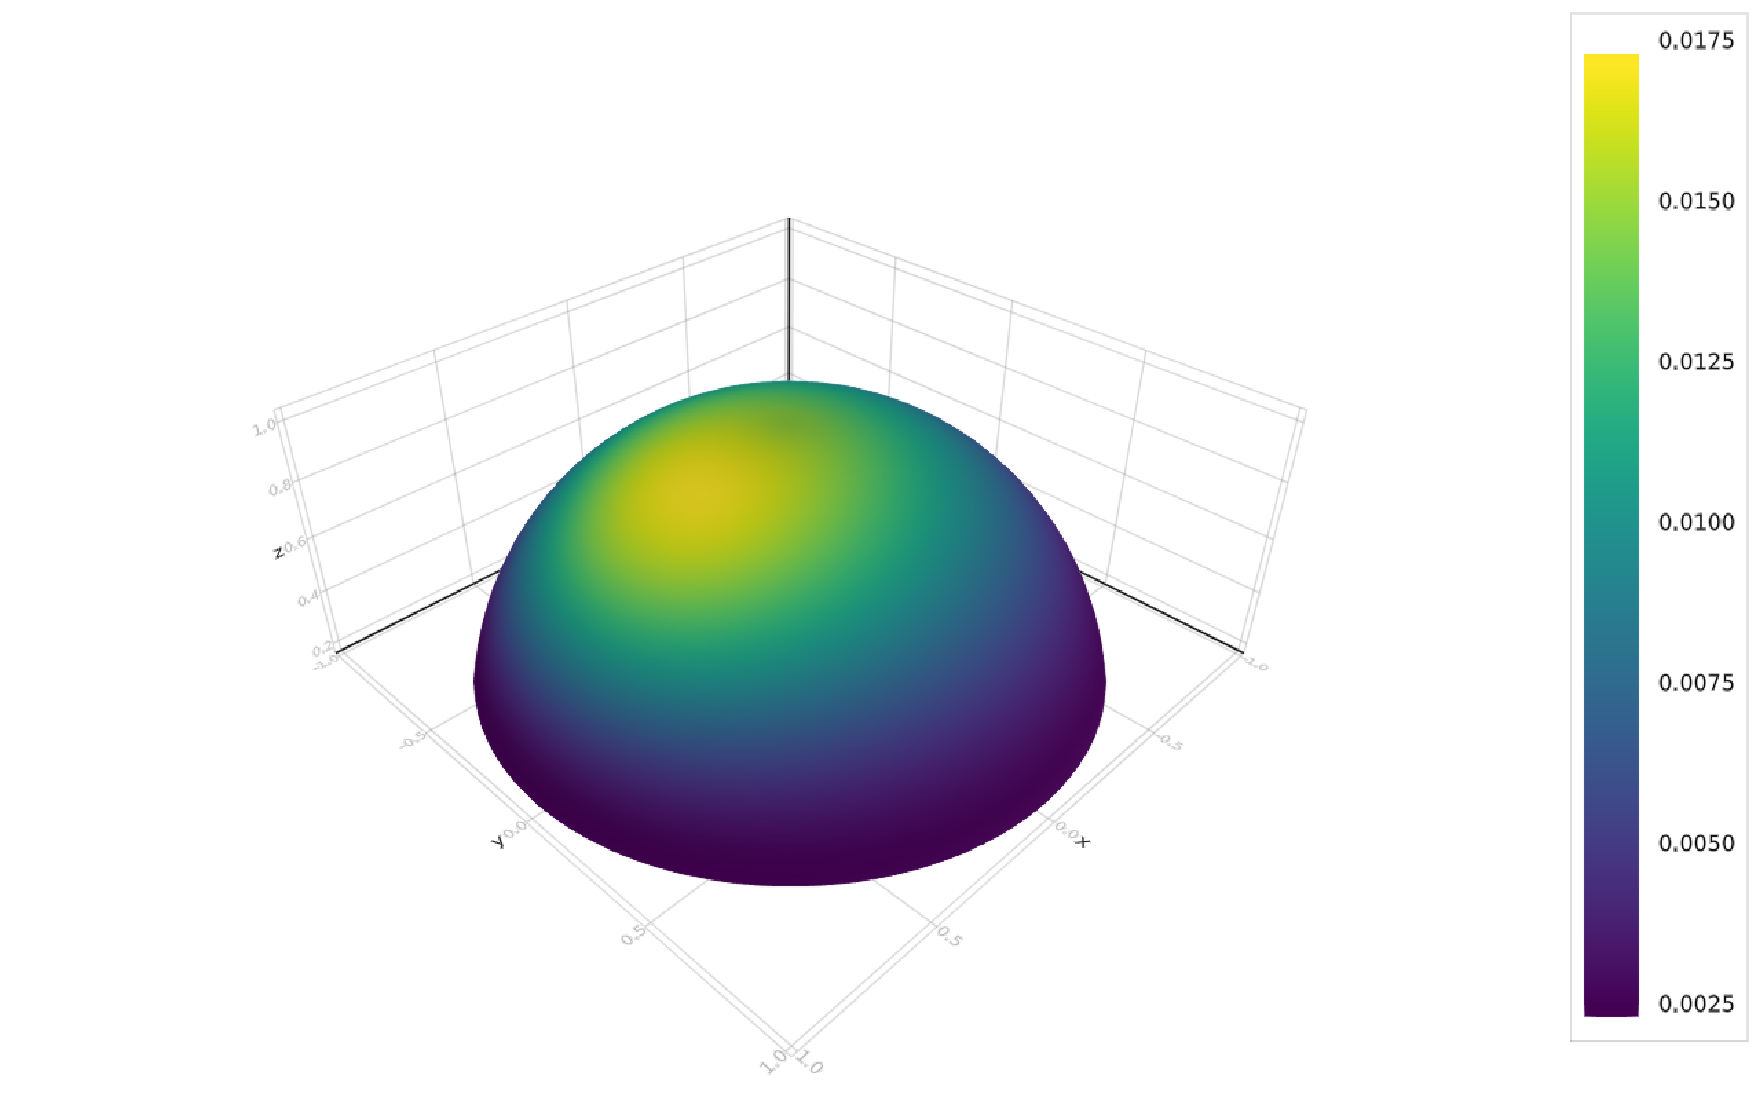
\includegraphics[scale=0.4]{biharmonic-f=erf-N=80-n=50}
	\end{subfigure}
	\hfill%
	
	\begin{subfigure}{0.55\textwidth}
		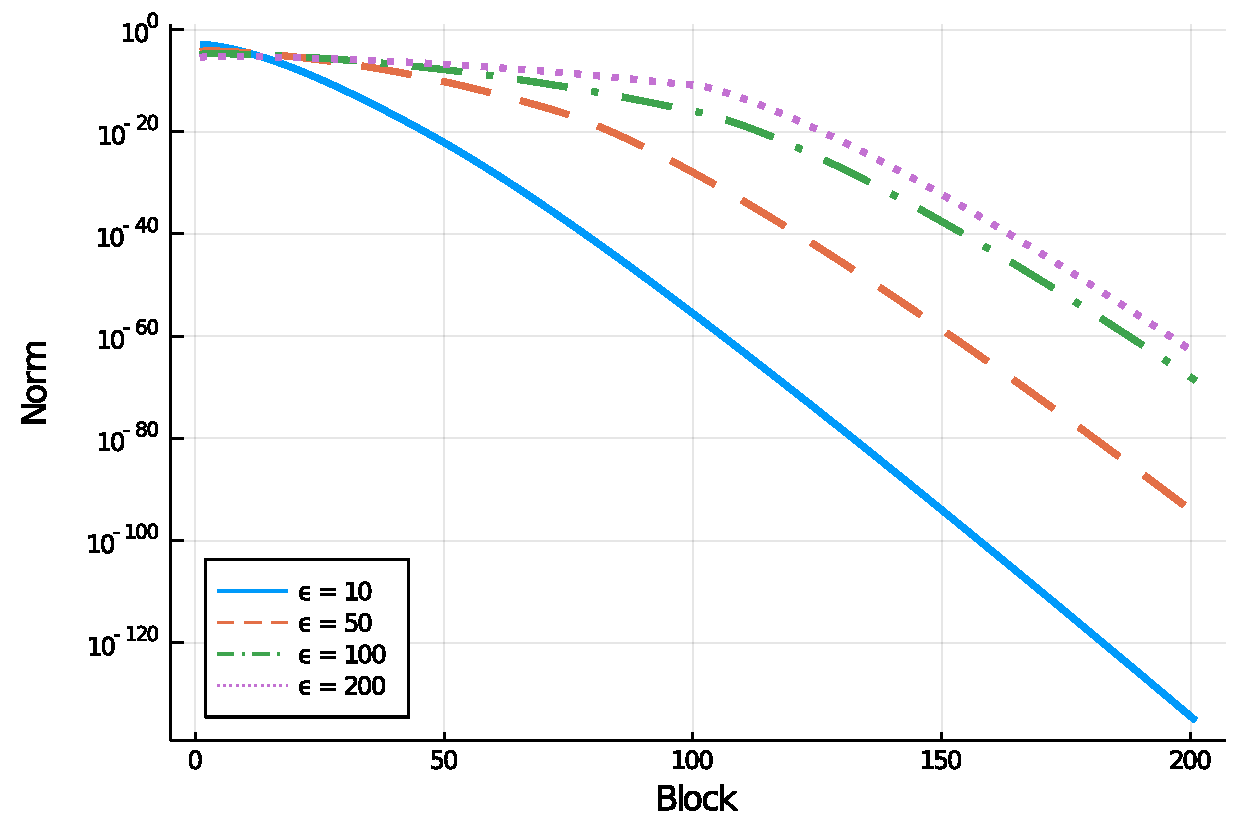
\includegraphics[scale=0.4]{solutionblocknorms-biharmonic-expfun-N=200}
	\end{subfigure}
	\hfill%
	\caption{Left: The computed solution to $\Delta^2 u = f$ with zero Dirichlet and Neumann boundary conditions with $f(x,y,z) = (1 + \text{erf}(5(1 - 10((x - 0.5)^2 + y^2)))) \rho(z)^2$. Right: The norms of each block of the computed solution of the biharmonic equation with the right hand side function $f(x,y,z) = \exp(-\epsilon((x-x_0)^2 + (y-y_0)^2 + (z-z_0)^2))$ where  $(x_0, z_0) := (0.7, 0.2)$, $y_0 := \sqrt{1 - x_0^2 - z_0^2}$, for various $\epsilon$ values. This demonstrates algebraic convergence.}
	\label{fig:sc:biharmonic}
\end{figure}

Our last example is the biharmonic equation: find $u(x,y,z)$ given a function $f(x,y,z)$ such that:
\bseqnnumber{
	\begin{cases}
    		\DeltaS^2 u(x,y,z) = f(x,y,z) &\quad \text{in } \Omega \\
		u(x,y,z) = 0, \quad \frac{\partial u}{\partial n}(x,y,z) = \grad_S \: u(x,y,z) \cdot \unitvec{n}(x,y,z) = 0 &\quad \text{on } \partial \Omega
	\end{cases}
	\label{eqn:sc:biharmonic}
}
where $\DeltaS^2$ is the Biharmonic operator, noting the imposition of zero Dirichlet and Neumann boundary conditions on $u$. For clarity, we reiterate that the unit normal vector in this sense is simply $\unitvec{n}(x,y,z) = \unitvec{n}(\vec x) := {\vec x \over \norm{\vec x}} = \vec x$ (see \bsrefsection{section:sc:furtherdiffoperators}). In \bsreffig{fig:sc:biharmonic} we see the solution to the Biharmonic \bsrefeqn{eqn:sc:biharmonic} in the spherical cap $\Omega$. In \bsreffig{fig:sc:biharmonic} we also show the norms of each block of calculated coefficients of the approximation for four more complex right-hand sides of the biharmonic equation with $N = 200$, that is, $(N+1)^2 = 40,401$ unknowns. Once again, the rate of decay in the coefficients is a proxy for the rate of convergence of the computed solution, and we see that we achieve exponential convergence for these more complex functions.


\subsection{Other boundary conditions}

One simple extension is the case where the value on the boundary takes that of a function depending only on $x$ and $y$, i.e. $c = c(x,y)$. In this case, the Helmholtz problem
\bseqn{
	\begin{cases}
    		\DeltaS u(x,y,z) + k^2 \: v(x,y,z) \; u(x,y,z) = f(x,y,z) &\quad \text{in } \Omega \\
		u(x,y,z) = c(x,y) &\quad \text{on } \partial \Omega
	\end{cases}
}
is equivalent to letting $u(x,y,z) = \tilde{u}(x,y,z)+ c(x,y)$ and solving
\bseqn{
	\begin{cases}
    		\DeltaS \tilde{u}(x,y,z) + k^2 \; v(x,y,z) \tilde{u}(x,y,z) = g(x,y,z) \quad \text{in } \Omega \\
		\tilde{u}(x,y,z) = 0 \quad \text{on } \partial \Omega
	\end{cases}
}
for $\tilde u$, where 
\bseqn{
	g(x,y,z) &:= f(x,y,z) - k^2 \: v(x,y,z) \: c(x,y) - \DeltaS \: c(x,y)
}
for $(x,y,z) \in \Omega$. This new problem is then a zero boundary condition Helmholtz problem with right hand side $g$. Notice that the spherical Laplacian applied to $c(x,y)$, expanded in the $\bigscopN^{(1)}$ basis with coefficients vector $\vec c = (c_{n,k,i})$, is just
\bseqn{
	\DeltaS \: c(x,y) &= {1 \over \rho(z)^2} \pmpxm{\theta}{2} c(x,y) \\
	&= {1 \over \rho(z)^2} \sum_{n=0}^N \sum_{i=0}^1 c_{n,n,i} \: \pmpxm{\theta}{2} \ch_{n,i}(\theta) \\
	&= - {1 \over \rho(z)^2} \sum_{n=0}^N \sum_{i=0}^1 n^2 \: c_{n,n,i} \: \ch_{n,i}(\theta)
}
since the coefficients $\{c_{n,k,i}\}$ for such a function are zero for $k < n$ due to the dependence on $x$ and $y$ only, which are precisely the Fourier coefficients of $c(\cos \theta, \sin \theta)$. Thus, since the function $c(x,y)$ is known, it is simple to evaluate $\pmpxm{\theta}{2} c(x,y)$ and hence one can obtain the coefficients for the expansion of $g(x,y,z)$ in the $\bigscopN^{(1)}$ basis in the usual manner.

Other boundary conditions beyond those already presented here are beyond the scope of this thesis. However, the approach established for the case of a triangle domain in 2D shows how Neumann conditions can be considered  as a system of equations in partial derivatives involving Dirchlet conditions \cite{olver2019triangle}. This approach may also work here for the spherical cap. Ideally, one would properly tackle the tangent bundle (that is defined in \bsrefdef{def:tangentbundle}) which would lower the degrees of freedom, but this is future work -- see \bsrefappendix{appendix:tangent}.



%
\section{Conclusions}

We have shown that trivariate orthogonal polynomials can lead to sparse discretizations of general linear PDEs on spherical cap domains, with Dirichlet boundary conditions on the $z = \alpha \in (0,1)$ boundary. We have provided a detailed practical framework for the application of the methods described for quadratic surfaces of revolution \cite{olver2020orthogonal}, by utilising the non-classical 1D OPs on the interval $[\alpha, 1]$ with the weight $(z - \alpha)^a \: (1-z^2)^{b/2}$ defined for the disk-slice case \cite{snowball2019sparse}. Generalisation to spherical bands ($\alpha \leq z \leq \beta$) is straightforward.  This work thus forms a building block in developing an $hp-$finite element method to solve PDEs on the sphere by using spherical band and spherical cap shaped elements.

This work also serves as a stepping stone to constructing similar methods to solve partial differential equations on other 3D sub-domains of the sphere such as spherical triangles. It is clear from the construction in this paper that discretizations spherical Laplacian's  and other partial differential operators are sparse on other suitable sub-components of the sphere. The resulting sparsity in high-polynomial degree discretizations presents an attractive alternative to methods based on bijective mappings (e.g., \cite{DGShallowWater,FEMShallowWater,boyd2005sphere}). Constructing these sparse spectral methods for surface PDEs on spherical triangles is future work, and has applications in weather prediction \cite{staniforth2012horizontal}, though it is not yet clear how to directly construct, or perhaps \textit{compute}, the necessary orthogonal polynomials. 

The next stage is to develop an orthogonal basis for the tangent bundle of the spherical cap (or band), and obtain sparse differential operators for the spherical gradient, divergence etc. On the complete sphere, the vector spherical harmonics that form the orthogonal basis are simply the gradients and perpendicular gradients of the scalar spherical harmonics \cite{barrera1985vector} which has been used effectively for solving PDEs on the sphere \cite{vasil2019tensor,lecoanet2019tensor} -- however, we do not have that luxury for the spherical cap or band, and hence the construction of a basis will not be as straightforward.







  










\chapter{Summary and future directions}

\section{Summary}

In this thesis, we have developed sparse spectral methods for solving partial differential equations (PDEs) on disk-slices and trapeziums in 2D, and spherical caps as a surface in 3D. The work can also be used as a template for developing similar methods on other such similar domains, in particular other subdomains of the sphere.

We began with an introduction to multidimensional sparse spectral methods by looking at the spherical harmonics on the whole sphere, explaining how they can be written as orthogonal polynomials in $x,y,z$, and how Jacobi and differential operators that apply to coefficient vectors will hence be banded-block-banded.

For the disk-slice in 2D, we defined the OPs that allow similar sparse and banded-block-banded operators required for solving PDEs in the domain, deriving their structure and providing a method to efficiently calculate numerically their entries. The reason they need to be calculated numerically is due to the non-classical univariate OPs that are involved in the 2D OP definitions. Finally, we moved on to use the same arguments for the spherical cap, a 3D surface that is a subdomain of the unit sphere. We once again defined the 3D OPs as orthogonal polynomials in $x,y,z$, and showed how the differential operator matrices continue to elicit similar banded-block-banded structure.


\section{Future directions}

We hope that this thesis can serve as somewhat of a blueprint for formalising sparse spectral methods, including how one should define the OPs and derive the accompanying Jacobi and differential operators. The motivation behind this work was to develop sparse spectral methods for subdomains of the unit sphere in 3D space. Thus, the natural direction from this point would be to formalise the framework for spherical bands, which would simply involve slightly more complex arithmetic and the sub-block bands would be slightly larger (this due to the $\genjac$ polynomials we defined now having no zero coefficients in their three-term recurrences, meaning the expressions for multiplication by $x,y,z$ would gain some extra terms).

A further avenue to take the framework for scalar functions is to construct a vector polynomial basis for functions whose values lie on the tangent bundle of the sphere. In \bsrefappendix{appendix:tangent}, we provide a summary for how one needs to approach this. The motivation for such is so as to be able to derive similarly sparsely structured operators for the spherical gradient and divergence. The main observation however is that, while the vector spherical harmonics are already established as being such an orthogonal and complete basis for the whole sphere, a similar construction for the spherical cap would not yield the same result.

Ideally, we would like to pair the framework presented in \bsrefchapter{CHAPTER:sphericalcaps} with a spectral element method for the sphere, where the elements would be the spherical subdomains of spherical bands and spherical caps. The goal here would be to test this method against the full sphere spectral method the is in place in the ECMWF model, with the hypothesis being that by reducing the size of the transforms, we can improve the overall efficiency while still maintaining the accuracy that we achieve from a spectral approach. 

Discretizations of partial differential operators are sparse on other suitable sub-domains of the sphere, as evidenced by the construction presented for the spherical cap. Hence, using the techniques learnt here, one could also look to constructing similar methods for solving PDEs on spherical triangles, with a view to using these sub-domains as elements for a spherical spectral element method. Moreover, one could use this framework to also develop sparse spectral methods on more general domains defined by an algebraic surface -- in particular those defined by non-uniform rational B-splines (NURBS). However, it is not obvious how one would derive or compute the OPs for such domains.









  








% END Thesis main body
%%%%%%%%%%


% appendices come here
\appendix

%%%%%%%%%%%%%%%%
%%% TANGENT SPACE %%%

\section{Vector-valued functions in the tangent space}

We can extend the methodology detailed in \bsrefchapter{CH:SCs} to the tangent space of the spherical cap $\Omega$, which we call $\tangentspace$. By creating a basis of orthogonal vector polynomials (OVPs) for the spherical cap $\Omega$, we can expand vector-valued functions that lie in the tangent space in this basis. Such functions that are useful for the sphere are gradients and perpendicular-gradients of scalar functions.

Any function in the tangent space of $\Omega$ can be written as $\nabla f + \rvec \times \nabla g$ for some scalar functions $f, g$ on $\Omega$. Let $f$ be a scalar function on $\Omega$ that satisfies zero boundary conditions. Then there exist coefficients $\vec{f}$ such that $f$ can be expanded in the OP basis $\bigW_N^{(1)}$ for large enough N, i.e. $f = \genjacw^{(1,0)} \: \sum_{n,k,i} f_{n,k,i} \: \scopnki^{(1)}$. The gradient and perpendicular gradient of $f$ are then
\begin{align*}
	\nabla f &= \sum_{n,k,i} f_{n,k,i} \: \nabla \Big( \genjacw^{(1,0)} \: \scopnki^{(1)} \Big) \\
	\rvec \times \nabla f &= \sum_{n,k,i} f_{n,k,i} \: \rvec \times \nabla \Big( \genjacw^{(1,0)} \: \scopnki^{(1)} \Big).
\end{align*}
For the whole sphere, recall from \bsrefsection{Section:VSHs} that we simply chose the vector spherical harmonics as our tangent space basis, defined as the gradient and perpendicular gradients of the scalar spherical harmonics. We could make that choice because the vector spherical harmonics as defined were naturally orthogonal. Unfortunately, we do not have the same luxury here, with the sets $\{ \nabla \Big( \genjacw^{(a,0)} \: \scopnki^{(a)} \Big), \rvec \times \nabla \Big( \genjacw^{(a,0)} \: \scopnki^{(a)} \Big) \}$ and $\{ \nabla \scopnki^{(a)}, \rvec \times \nabla \scopnki^{(a)} \}$ not being orthogonal for any parameter $a$. The game for future work is to find an orthogonal basis that spans the tangent space of the spherical cap $\Omega$, such that we can sparsely expand the likes of $\nabla \scopnki^{(a)}$.




%%%%%

%We can extend the methodology detailed in \bsrefchapter{CH:SCs} to the tangent space of the spherical cap $\Omega$, which we call $\tangentspace$. By creating a basis of orthogonal vector polynomials (OVPs) for the spherical cap $\Omega$, we can expand vector-valued functions that lie in the tangent space in this basis. Such functions that are useful for the sphere are gradients and perpendicular-gradients of scalar functions. In this section we will define the OVPs, outline the Clenshaw matrices and how to build the OVFs, function evaluation as well as differential operators for gradient, curl and divergence that take us to and from coefficients in either of the OVP or scalar OP expansions.
%
%Any function in the tangent space of $\Omega$ can be written as $\nabla f + \rvec \times \nabla g$ for some scalar functions $f, g$ on $\Omega$. Let $f$ be a scalar function on $\Omega$ that satisfies zero boundary conditions. Then there exist coefficients $\bm{f}$ such that $f$ can be expanded in the OP basis $\bigW_N^{(1)}$ for large enough N, i.e. $f = \genjacw^{(1,0)} \: \sum_{n,k,i} f_{n,k,i} \: \scopnki^{(1)}$. The gradient and perpendicular gradient of $f$ are then
%\begin{align*}
%	\nabla f &= \sum_{n,k,i} f_{n,k,i} \: \nabla \Big( \genjacw^{(1,0)} \: \scopnki^{(1)} \Big) \\
%	\rvec \times \nabla f &= \sum_{n,k,i} f_{n,k,i} \: \rvec \times \nabla \Big( \genjacw^{(1,0)} \: \scopnki^{(1)} \Big).
%\end{align*}
%For the whole sphere, recall from \bsrefsection{Section:VSHs} that we simply chose the vector spherical harmonics as our tangent space basis, defined as the gradient and perpendicular gradients of the scalar spherical harmonics. We could make that choice because the vector spherical harmonics as defined were naturally orthogonal. Unfortunately, we do not have the same luxury here, with the sets $\{ \nabla \Big( \genjacw^{(a,0)} \: \scopnki^{(a)} \Big), \rvec \times \nabla \Big( \genjacw^{(a,0)} \: \scopnki^{(a)} \Big) \}$ and $\{ \nabla \scopnki^{(a)}, \rvec \times \nabla \scopnki^{(a)} \}$ not being orthogonal for any parameter $a$. 
%
%The game is to find an orthogonal basis that spans the tangent space of the spherical cap $\Omega$ such that we can sparsely expand $\nabla \Big( \genjacw^{(1,0)} \: \scopnki^{(1)} \Big)$ and $\rvec \times \nabla \Big( \genjacw^{(1,0)} \: \scopnki^{(1)} \Big)$ for each $n,k,i$ trio.
%
%Define the OVFs as follows:
%\begin{align}
%	\tsopinki(x,y,z) &:= \phivec \: \frac{1}{\rho(z)} \: \scopnki^{(0)}(x,y,z) \\
%	\tsopiinki(x,y,z) &:= \thetavec \: \frac{1}{\rho(z)} \: \scopnki^{(0)}(x,y,z)
%\end{align}
%where
%\begin{align}
%	\phivec &:= 
%		\begin{pmatrix}
%			\cos(\theta) \: \cos(\phi) \\
%			\sin(\theta) \: \cos(\phi) \\
%			- \sin(\phi)
%		\end{pmatrix}
%		=
%		\begin{pmatrix}
%			x z / \rho(z) \\
%			y z / \rho(z) \\
%			- \rho(z)
%		\end{pmatrix} \\
%	\thetavec &:= 
%		\begin{pmatrix}
%			-\sin(\theta) \\
%			\cos(\theta) \\
%			0
%		\end{pmatrix}
%		=
%		\begin{pmatrix}
%			-y / \rho(z) \\
%			x / \rho(z) \\
%			0
%		\end{pmatrix}
%\end{align}
%These are orthogonal with respect to the inner product $\ip<\bm{A}, \bm{B}>_\tangentspace := \int_\Omega \bm{A} \cdot \bm{B} \: \rho(z)^2 \: \D A$:
%\begin{align*}
%	\ip<\tsopinki, \tsopi_{m,j,h}>_\tangentspace &= \int_\Omega \tsopinki \cdot \tsopi_{m,j,h} \: \rho(z)^2 \:\D A \\
%	&= \int_\Omega \scopnki^{(0)} \: \scopmjh^{(0)} \: \D \Omega \\
%	&= \pi \: \normgenjac^{(0, 2k)} \: \delta_{n,m} \: \delta_{k,j} \: \delta_{i,h}, \\
%	\ip<\tsopiinki, \tsopii_{m,j,h}>_\tangentspace &= \int_\Omega \tsopiinki \cdot \tsopii_{m,j,h} \: \rho(z)^2 \:\D A \\
%	&= \int_\Omega \scopnki^{(0)} \: \scopmjh^{(0)} \: \D \Omega \\
%	&= \pi \: \normgenjac^{(0, 2k)} \: \delta_{n,m} \: \delta_{k,j} \: \delta_{i,h}, \\
%	\ip<\tsopinki, \tsopii_{m,j,h}>_\tangentspace &\equiv 0.
%\end{align*}
%To show that these span the tangent space $\tangentspace$, we merely require that we can sparsely expand $\nabla \Big( \genjacw^{(1,0)} \: \scopnki^{(1)} \Big), \: \rvec \times \nabla \Big( \genjacw^{(1,0)} \: \scopnki^{(1)} \Big)$ with the vectors $\tsopi_{m,j,h}, \tsopii_{m,j,h}$.  First, note that
%\begin{align*}
%	\nabla \Big( \genjacw^{(1,0)} \: \scopnki^{(1)} \Big) &= \phivec \: \ppphi \Big( \genjacw^{(1,0)} \: \scopnki^{(1)} \Big) + \thetavec \: \frac{1}{\rho(z)} \: \pptheta \Big( \genjacw^{(1,0)} \: \scopnki^{(1)} \Big) \\
%	&= \phivec \: \Big[k \: z \: \genjacw^{(1,0)}(z) \: \genjacnmk^{(1,2k)}(z) -  \big(\genjacw^{(1,0)}(z) \: \genjacnmk^{(1,2k)}(z) \big)' \rho(z)^2 \Big] \: \rho(z)^{k-1} \: \chki(\theta) \\
%	&\quad \quad + \thetavec \: (-1)^{i+1} \: k \: \genjacw^{(1,0)}(z) \: \genjacnmk^{(1,2k)}(z) \: \rho(z)^{k-1} \: \ch_{k,|i-1|}(\theta).
%\end{align*}
%Then,
%\begin{align*}
%	&\ip<\nabla \Big( \genjacw^{(1,0)} \: \scopnki^{(1)} \Big), \tsopi_{m,j,h}>_\tangentspace \\
%	&\quad \quad = \int_\Omega \nabla \Big( \genjacw^{(1,0)} \: \scopnki^{(1)} \Big) \cdot \tsopi_{m,j,h} \: \rho(z)^2 \:\D A \\
%	&\quad \quad = \pi \: \delta_{k,j} \: \delta_{i,h} \: \int_\alpha^1 \Big[k \: z \: \genjacw^{(1,0)} \: \genjacnmk^{(1,2k)} -  (\genjacw^{(1,0)} \: \genjacnmk^{(1,2k)})' \rho^2 \Big] \: \rho^{k-1} \: \genjac_{m-k}^{(0,2k)} \: \rho^{k-1} \: \rho^2 \:\D z \\
%	&\quad \quad = \pi \: \delta_{k,j} \: \delta_{i,h} \: \int_\alpha^1 \Big[k \: z \: \genjacw^{(1,0)} \: \genjacnmk^{(1,2k)} -  (\genjacw^{(1,0)} \: \genjacnmk^{(1,2k)})' \rho^2 \Big] \: \genjac_{m-k}^{(0,2k)} \: \rho^{2k} \:\D z \quad (\star) \\
%	&\quad \quad = \pi \: \delta_{k,j} \: \delta_{i,h} \: \int_\alpha^1 \Big( kz \: \genjacnmk^{(1,2k)} \: \genjac_{m-k}^{(0,2k)} \: \genjacw^{(1,2k)} \\
%	&\quad \quad\quad \quad\quad \quad\quad \quad\quad \quad+ \genjacw^{(1,2k)} \: \genjacnmk^{(1,2k)} \: \Big[ \genjac_{m-k}^{(0,2k) \; \prime} \: \rho^2 - (2k+2) \: z \: \genjac_{m-k}^{(0,2k)} \Big] \Big) \: \D z \\
%	&\quad \quad = \pi \: \delta_{k,j} \: \delta_{i,h} \: \int_\alpha^1 \genjacnmk^{(1,2k)} \: \Big[ - (k + 2) \: z \: \genjac_{m-k}^{(0,2k)} + \genjac_{m-k}^{(0,2k) \; \prime} \: \rho^2 \Big] \: \genjacw^{(1,2k)} \: \D z \quad (\star \star)
%\end{align*}
%where by orthogonality of the $\{\genjac_n^{(a,2b)}\}$ OPs we have that the above is zero for $m - k > n - k + 2 \iff m > n + 2$ at $(\star)$ and also for $n - k > m - k + 1 \iff m < n - 1$ at $(\star \star)$. Further, 
%\begin{align*}
%	&\ip<\nabla \Big( \genjacw^{(1,0)} \: \scopnki^{(1)} \Big), \tsopii_{m,j,h}>_\tangentspace \\
%	&\quad \quad = \int_\Omega \nabla \Big( \genjacw^{(1,0)} \: \scopnki^{(1)} \Big) \cdot \tsopii_{m,j,h} \: \rho(z)^2 \:\D A \\
%	&\quad \quad = (-1)^{i+1} \: k \: \pi \: \delta_{k,j} \: \delta_{i,|h-1|} \: \int_\alpha^1 \genjacw^{(1,0)} \: \genjacnmk^{(1,2k)} \: \rho^{k-1} \: \genjac_{m-k}^{(0,2k)} \: \rho^{k-1} \: \rho^2 \:\D z \\
%	&\quad \quad = (-1)^{i+1} \: k \: \pi \: \delta_{k,j} \: \delta_{i,|h-1|} \: \int_\alpha^1 \genjacnmk^{(1,2k)}  \: \genjac_{m-k}^{(0,2k)} \: \genjacw^{(1,2k)} \: \D z
%\end{align*}
%which again by orthogonality is zero for $m - k > n - k + 1 \iff m > n + 1$ and $n - k > m - k \iff m < n$. We of course have similar results for $\rvec \times \nabla \Big( \genjacw^{(1,0)} \: \scopnki^{(1)} \Big)$ since
%\begin{align*}
%	\rvec \times \phivec = \thetavec, \quad \rvec \times \thetavec = - \phivec.
%\end{align*}
%We now have a set of orthogonal vector valued functions that span the tangent space $\tangentspace$. By construction, we have the same recurrence coefficients for multiplication by $x,y,z$ for each of the OVFs as for the OPs $\scopnki^{(0)}$. 
%
%Define
%\begin{align*}
%	\bigtsoptn := 
%		\begin{pmatrix}
%			\tsopit_{n,0,0}(x,y,z) \\
%			\tsopiit_{n,0,0}(x,y,z) \\
%			\tsopit_{n,1,0}(x,y,z) \\
%			\tsopiit_{n,1,0}(x,y,z) \\
%			\tsopit_{n,1,1}(x,y,z) \\
%			\tsopiit_{n,1,1}(x,y,z) \\
%			\vdots \\
%			\tsopit_{n,n,0}(x,y,z) \\
%			\tsopiit_{n,n,0}(x,y,z) \\
%			\tsopit_{n,n,1}(x,y,z) \\
%			\tsopiit_{n,n,1}(x,y,z)
%		\end{pmatrix} \in \R^{2(2n+1) \times 3}, 
%	\quad \quad 
%	\bigtsopt := 
%		\begin{pmatrix}
%			\bigtsopt_0 \\
%			\bigtsopt_1 \\
%			\bigtsopt_2 \\
%			\vdots \\
%		\end{pmatrix}
%\end{align*}
%and set $\jacobimattangentx, \jacobimattangenty, \jacobimattangentz$ as the Jacobi matrices corresponding to
%\begin{align}
%	\jacobimattangentx \: \bigtsopt(x,y,z) = x \: \bigtsopt(x,y,z), \nonumber \\
%	\jacobimattangenty \: \bigtsopt(x,y,z) = y \: \bigtsopt(x,y,z), \label{eqn:jacobimatricestangentdefinition} \\
%	\jacobimattangentz \: \bigtsopt(x,y,z) = z \: \bigtsopt(x,y,z), \nonumber
%\end{align}
%The matrices $\jacobimattangentx, \jacobimattangenty, \jacobimattangentz$ act on the coefficients vector of a function's expansion in the $\bigtsopt$ basis. For example, let a function $\bm{F}(x,y,z) : \Omega \to \tangentspace$ be approximated by its expansion $\bm{F}(x,y,z)^\top = \bigtsopt(x,y,z)^\top \bm{F}_c$, for some coefficients vector $\bm{F}_c$. Then $x \: \bm{F}(x,y,z)$ is approximated by $\bigtsopt(x,y,z)^\top {(\jacobimattangentx)}^\top \bm{F}_c$. In other words, ${(\jacobimattangentx)}^\top \bm{F}_c$ is the coefficients vector for the expansion of the function $(x,y,z) \mapsto x \: \bm{F}(x,y,z)$ in the  $\bigtsopt$ basis. Further, note that $\jacobimattangentx, \jacobimattangenty, \jacobimattangentz$ are banded-block-banded matrices -- they are block-tridiagonal (block-bandwidths $(1,1)$):
%\begin{align*}
%	\jacobimattangent_{x/y/z} &= 
%		\begin{pmatrix}
%			B_{x/y/z, 0} & A_{x/y/z, 0} & & & & \\
%			C_{x/y/z, 1} & B_{x/y/z, 1} & A_{x/y/z, 1} & & & \\
%			& C_{x/y/z, 2} & B_{x/y/z, 2} & A_{x/y/z, 2} & & & \\
%			& & C_{x/y/z, 3} & \ddots & \ddots & \\
%			& & & \ddots & \ddots & \ddots \\
%		\end{pmatrix}
%\end{align*}
%For $\jacobimattangentx$, the sub-blocks have sub-block-bandwidths $(?,?)$:
%\begin{align*}
%	A_{x,n} &:= 
%		\begin{pmatrix}
%			0 & A_{n,0,6} & 0 & & \\
%			A_{n,1,5} & \ddots & \ddots & & \\
%			& \ddots & \ddots & \ddots & \\
%			& & A_{n,n,5} & 0 & A_{n,n,6} \\
%		\end{pmatrix} \in \R^{2(2n+1)\times2(2n+3)}, \quad n = 0,1,2,\dots \\
%	B_{x,n} &:= 
%		\begin{pmatrix}
%			0 & A_{n,0,4} & & \\
%			A_{n,1,3} & \ddots & \ddots & \\
%			& \ddots & \ddots & A_{n,n-1,4} \\
%			& & A_{n,n,3} & 0
%		\end{pmatrix} \in \R^{2(2n+1)\times2(2n+1)}  \quad n = 0,1,2,\dots \\
%	C_{x,n} &:= 
%		\begin{pmatrix}
%			0 & A_{n,0,2} & & \\
%			A_{n,1,1} & \ddots & \ddots & \\
%			& \ddots & \ddots & A_{n,n-2,2} \\
%			& & \ddots & 0 \\
%			& & & A_{n,n,1} \\
%		\end{pmatrix} \in \R^{2(2n+1)\times2(2n-1)}, \quad n = 1,2,\dots
%\end{align*}
%where
%\begin{align*}
%	A_{n,k,j} &:= \alphaonkj \: I_{4} \in \R^{4\times4}, \quad k = 1,\dots,n \: (j \text{ even}), \quad k = 2,\dots,n \: (j \text{ odd}) \\
%	A_{n,0,j} &:=
%		\begin{pmatrix}
%			\alphao_{n,0,j} & 0 & 0 & 0 \\
%			0 & \alphao_{n,0,j} & 0 & 0
%		\end{pmatrix} \in \R^{2\times4}, \quad j \text{ even} \\
%	A_{n,1,j} &:=
%		\begin{pmatrix}
%			\alphao_{n,1,j} & 0 \\
%			0 & \alphao_{n,1,j} \\
%			0 & 0 \\
%			0 & 0
%		\end{pmatrix} \in \R^{4\times2}, \quad j \text{ odd}
%\end{align*}
%For $\jacobimattangenty$, the sub-blocks have sub-block-bandwidths $(?,?)$:
%\begin{align*}
%	A_{y,n} &:= 
%		\begin{pmatrix}
%			0 & B_{n,0,6} & 0 & & \\
%			B_{n,1,5} & \ddots & \ddots & & \\
%			& \ddots & \ddots & \ddots & \\
%			& & B_{n,n,5} & 0 & B_{n,n,6} \\
%		\end{pmatrix} \in \R^{2(2n+1)\times2(2n+3)}, \quad n = 0,1,2,\dots \\
%	B_{y,n} &:= 
%		\begin{pmatrix}
%			0 & B_{n,0,4} & & \\
%			B_{n,1,3} & \ddots & \ddots & \\
%			& \ddots & \ddots & B_{n,n-1,4} \\
%			& & B_{n,n,3} & 0
%		\end{pmatrix} \in \R^{2(2n+1)\times2(2n+1)}  \quad n = 0,1,2,\dots \\
%	C_{y,n} &:= 
%		\begin{pmatrix}
%			0 & B_{n,0,2} & & \\
%			B_{n,1,1} & \ddots & \ddots & \\
%			& \ddots & \ddots & B_{n,n-2,2} \\
%			& & \ddots & 0 \\
%			& & & B_{n,n,1} \\
%		\end{pmatrix} \in \R^{2(2n+1)\times2(2n-1)}, \quad n = 1,2,\dots
%\end{align*}
%where
%\begin{align*}
%	B_{n,k,j} &:= 
%		\begin{pmatrix}
%			0 & 0 & \betaonkj & 0 \\
%			0 & 0 & 0 & \betaonkj \\
%			\betaonkj & 0 & 0 & 0 \\
%			0 & \betaonkj & 0 & 0
%		\end{pmatrix} \in \R^{4\times4}, \quad k = 1,\dots,n \: (j \text{ even}), \quad k = 2,\dots,n \: (j \text{ odd}) \\
%	B_{n,0,j} &:=
%		\begin{pmatrix}
%			0 & 0 & \betao_{n,0,j} & 0 \\
%			0 & 0 & 0 & \betao_{n,0,j}
%		\end{pmatrix} \in \R^{2\times4}, \quad j \text{ even} \\
%	B_{n,1,j} &:=
%		\begin{pmatrix}
%			0 & 0 \\
%			0 & 0 \\
%			\betao_{n,1,j} & 0 \\
%			0 & \betao_{n,1,j}
%		\end{pmatrix} \in \R^{4\times2}, \quad j \text{ odd}
%\end{align*}
%For $\jacobimattangentz$, the sub-blocks have sub-block-bandwidths $(?,?)$:
%\begin{align*}
%	A_{z,n} &:= 
%		\begin{pmatrix}
%			\Gamma_{n,0,3} & 0 & 0 & & \\
%			0 & \ddots & \ddots & & \\
%			& \ddots & \ddots & \ddots & \\
%			& & 0 & \Gamma_{n,n,3} & 0 \\
%		\end{pmatrix} \in \R^{2(2n+1)\times2(2n+3)}, \quad n = 0,1,2,\dots \\
%	B_{z,n} &:= 
%		\begin{pmatrix}
%			\Gamma_{n,0,2} & 0 & & \\
%			0 & \ddots & \ddots & \\
%			& \ddots & \ddots & 0 \\
%			& & 0 & \Gamma_{n,n,2}
%		\end{pmatrix} \in \R^{2(2n+1)\times2(2n+1)}  \quad n = 0,1,2,\dots \\
%	C_{z,n} &:= 
%		\begin{pmatrix}
%			\Gamma_{n,0,1} & 0 & & \\
%			0 & \ddots & \ddots & \\
%			& \ddots & \ddots & 0 \\
%			& & \ddots &  \Gamma_{n,n-1,1} \\
%			& & & 0 \\
%		\end{pmatrix} \in \R^{2(2n+1)\times2(2n-1)}, \quad n = 1,2,\dots
%\end{align*}
%where
%\begin{align*}
%	\Gamma_{n,k,j} &:= \gammaonkj \: I_{4} \in \R^{4\times4}, \quad k = 1,\dots,n \\
%	\Gamma_{n,0,j} &:=
%		\begin{pmatrix}
%			\gammao_{n,0,j} & 0 \\
%			0 & \gammao_{n,0,j}
%		\end{pmatrix} \in \R^{2\times2}.
%\end{align*}
%Note that the sparsity of the Jacobi matrices (in particular the sparsity of the sub-blocks) comes from the natural sparsity of the three-term recurrences of the 1D OPs and the circular harmonics, meaning that the sparsity is not limited to the specific spherical cap, and would extend to the spherical band.
%
%
%\subsection{Building the OPs} 
%
%We can combine each system in (\ref{eqn:jacobimatricestangentdefinition}) into a block-tridiagonal system, for any $(x,y,z) \in \Omega$:
%
%\begin{align*}
%\renewcommand\arraystretch{1.3}
%\begin{pmatrix}
%		I_2 & & & \\
%		B_0-G_0(x,y,z) & A_0 & & \\
%		C_1 & B_1-G_1(x,y,z) & \quad A_1 \quad & \\
%		& C_2 & B_2 - G_2(x,y,z)  & \ddots \\
%		& & \ddots &\ddots
%\end{pmatrix}
%\bigtsopt(x,y,z)
%=
%\begin{pmatrix}
%	 \tsopi_0^\top \\ \tsopii_0^\top \\ 0 \\ 0 \\ \vdots  \\
%\end{pmatrix},
%\end{align*}
%where we note $\scopa_0 := \scopa_{0,0,0}(x,y,z) \equiv \genjac_0^{(a,0)} \: \ch_0$, and for each $n = 0,1,2\dots$,
%\begin{align*}
%A_n &:= \begin{pmatrix}
%		A_{x,n} \\
%		A_{y,n} \\
%		A_{z,n}
%	    \end{pmatrix} \in \R^{6(2n+1)\times2(2n+3)}, \quad
%C_n := \begin{pmatrix}
%		C_{x,n} \\
%		C_{y,n} \\
%		C_{z,n}
%	    \end{pmatrix} \in \R^{6(2n+1)\times2(2n-1)} \quad (n \ne 0), \nonumber \\
%B_n &:= \begin{pmatrix}
%		B_{x,n} \\
%		B_{y,n} \\
%		B_{z,n}
%	    \end{pmatrix} \in \R^{6(2n+1)\times2(2n+1)}, \quad
%G_n(x,y,z) := \begin{pmatrix}
%		xI_{2(2n+1)} \\
%		yI_{2(2n+1)} \\
%		zI_{2(2n+1)}
%	    \end{pmatrix} \in \R^{6(2n+1)\times2(n+1)}.
%\end{align*}
% 
%For each $n = 0,1,2\dots$ let $\Dnt$ be any matrix that is a left inverse of $A_n$, i.e. such that $\Dnt A_n = I_{2(2n+3)}$. Multiplying our system by the preconditioner matrix that is given by the block diagonal matrix of the $\Dnt$'s, we obtain a lower triangular system \cite[p78]{dunkl2014orthogonal}, which can be expanded to obtain the recurrence:
%\begin{align*}
%	\begin{cases}
%		\bigtsopt_{-1}(x,y,z) := 0 \\
%		\bigtsopt_{0}(x,y,z) = 
%			\begin{pmatrix} 
%				\tsopi_0^\top \\ 
%				\tsopii_0^\top
%			\end{pmatrix} :=
%			\begin{pmatrix} 
%				\tsopi_{0,0,0}^\top \\
%				\tsopi_{0,0,0}^\top
%			\end{pmatrix} \\
%		\bigtsopt_{n+1}(x,y,z) = -\Dnt (B_n-G_n(x,y,z)) \bigtsoptn(x,y,z) - \Dnt C_n  \, \bigtsopt_{n-1}(x,y,z), \quad n = 0,1,2,\dots.
%	\end{cases}
%\end{align*}
%
%Note that we can define an explicit \(\Dnt\) as follows: \bstodo{type up DnT for tangent space}
%\begin{align*}
%\Dnt := \begin{pmatrix}
%		0 & & & 0 & & & 1 / \gammaa_{n,0,3} & & \\
%		& \ddots & & & \ddots & & & \ddots \\
%		& & \ddots & & & \ddots & & & \ddots \\
%		& & & 0 & & & 0 & & & 1 / \gammaa_{n,n,3}  \\
%		& & & & & \bm{\eta}^\top_{1} & & & \\
%		& & & & & \bm{\eta}^\top_{0} & & &
%	    \end{pmatrix} \in \R^{(2n+3)\times3(2n+1)},
%\end{align*}
%for $n = 2, 3, \dots$ where $\bm{\eta}_{0}, \bm{\eta}_{1} \in \R^{3(2n+1)}$ with entries given by 
%\begin{align*}
%	\big(\bm{\eta}_{0}\big)_j &= 
%		\begin{cases}
%			\frac{1}{\alphaa_{n,n,6}} & j = 2n+1 \\
%			\frac{- \: \alphaa_{n,n,5}}{\alphaa_{n,n,6} \: \gammaa_{n, n-1, 3}} & j = 3(2n+1) - 2 \\
%			0 & o/w
%		\end{cases} \\
%	\big(\bm{\eta}_{1}\big)_j &= 
%		\begin{cases}
%			\big(\bm{\eta}_{0}\big)_{j+1} & j = 2n, 3(2n+1) - 3 \\
%			0 & o/w
%		\end{cases}
%\end{align*}
%For $n=0, 1$, we can simply take
%\begin{align*}
%D^\top_0 &:= \begin{pmatrix}
%		0 & 0 & \frac{1}{\gammaa_{0,0,3}} \\
%		\frac{1}{\alphaa_{0,0,6}} & 0 & 0 \\
%		0 & \frac{1}{\betaa_{0,0,6}} & 0
%	    \end{pmatrix} \in \R^{3\times3}, \\
%D^\top_1 &:= \begin{pmatrix}
%		0 & 0 & 0 & 0 & 0 & 0 & 1 / \gammaa_{1,0,3} & & \\
%		0 & 0 & 0 & 0 & 0 & 0 & 0 & 1 / \gammaa_{1,1,3} \\
%		0 & 0 & 0 & 0 & 0 & 0 & 0 & 0 & 1 / \gammaa_{1,1,3}  \\
%		0 & 1 / \alphaa_{1,1,6} & 0 & 0 & 0 & 0 & \eta & 0 & 0 \\
%		0 & 0 & 1 / \alphaa_{1,1,6} & 0 & 0 & 0 & 0 & 0 & 0
%	    \end{pmatrix} \in \R^{5\times9},
%\end{align*}
%where $\eta = \frac{- \: \alphaa_{1,1,5}}{\alphaa_{1,1,6} \: \gammaa_{1, 0, 3}}$.
%
%It follows that we can apply $\Dnt$ in $O(n)$ complexity, and thereby calculate $\bigtsopt_0(x,y,z)$  through $\bigtsoptn(x,y,z)$ in optimal $O(n^2)$ complexity. \bstodo{correct for this case}
%
%\subsection{Operators}
%
%Gradient operator on a scalar function is pretty much outlined above. Divergence would either be worked out by knowing what $f,g$ are for a function $\bm{F} = \nabla f + \rvec \times \nabla g$, so that $\nabla \cdot \bm{F} = \nabla^2 f$. Alternatively, we have expressions for $\rhoppphi \scopnkia$ and $\pptheta \scopnkia$ so that we can calculate an operator for $\rho^2 \nabla \cdot$, i.e. 
%\begin{align*}
%	\rho^2 \nabla \cdot \bm{F} &= \rho^2 \: \frac{1}{\rho} \ppphi (\rho F^\phi) + \rho^2 \: \frac{1}{\rho} \pptheta F^\theta \\
%	&= \sum_{n,k,i} F^\phi_{n,k,i} \: \rhoppphi \scopnki^{(0)} + F^\theta_{n,k,i} \: \pptheta \scopnki^{(0)}.
%\end{align*}
%
%
%\subsection{Linear SWE}
%
%\begin{align*}
%	\uvec_t &= - f \rvec \times \uvec + \grad h \\
%	h_t &= -\href \divergence \uvec
%\end{align*}
%$\implies$
%\begin{align*}
%	\uvecnpi &= \uvecn - \Delta t \: f \rvec \times \uvecnpi +\Delta t \: \grad h_{n+1} \\
%	h_{n+1} &= h_n - \Delta t \: \href \divergence \uvecnpi
%\end{align*}
%$\implies$
%\begin{align*}
%	\uvecnpic &= \uvecnc - \Delta t \: F \uvecnpic +\Delta t \: G \hvecnpic \\
%	P \hvecnpic &= P \hvecnc - \Delta t \: \href D \uvecnpic
%\end{align*}
%where $F : \bigtsop \to \bigtsop$ is the operator for $f \rvec \times$, $D : \bigtsop \to \bigscop^{(1)}$ is the operator for $\rho^2 \divergence$, $G : \bigW^{(1)} \to \bigtsop$ is the operator for $\grad$, and $P : \bigW^{(1)} \to \bigscop^{(1)}$ is the operator for multiplication by $\rho(z)^2$.
%
%
%
%
%
%
%  










% notation index here
\newpage
\addcontentsline{toc}{chapter}{Index of Notation}
\printnomenclature


% References
\newpage
\addcontentsline{toc}{chapter}{Bibliography}
%\bibliographystyle{alpha}
\bibliography{bibliography/thesis-ben-snowball}


\end{document}





  







